%%%%%%%%%%%%%%%%%%%%%%%%%%%%%%%%%%%%%%%%%
% OIST Doctoral Thesis
% LaTeX Template
% Version 0.3 (2018/03)
%
% Original author:
% Jeremie Gillet
%
%%%%%%%%%%%%%%%%%%%%%%%%%%%%%%%%%%%%%%%%%

%-------------------------------------------------------------------------------
%	REQUIRED PACKAGES AND  CONFIGURATIONS
%-------------------------------------------------------------------------------
\documentclass[final]{oist_thesis} % Final version for thesis submission

% The documentclass oist_thesis includes the following packages: geometry, caption, xkeyval

\usepackage[english]{babel} % The document is in English
\usepackage[utf8]{inputenc} % UTF8 encoding
\usepackage[T1]{fontenc} % Font encoding

\usepackage{graphicx} % For including images
\graphicspath{{./Images/}} % Specifies the directory where pictures are stored

\usepackage{eso-pic} % For the background picture on the title page

\usepackage{setspace} % For using single or double spacing
\usepackage{longtable} % tables that can span several pages
\usepackage{pdfpages} % To include a pdf files of your published papers as an appendix
\usepackage{fancyhdr} % For the headers
\usepackage[hidelinks]{hyperref} % Adds clickable links at references
\usepackage{subcaption}

%----------------------------------------------------------------------------------------
%	ADD YOUR PACKAGES (be careful of package interaction)
%----------------------------------------------------------------------------------------

\usepackage{amsthm, amsmath, amssymb, amsfonts, bbm, bm} % Math symbols
\usepackage{fontspec} % More fonts
% \usepackage[parfill]{parskip} % Gaps instead of indents
\usepackage{gensymb} % \degree symbol
\usepackage{lipsum}% http://ctan.org/pkg/lipsum
\usepackage{flafter}
\usepackage{notoccite}
\usepackage{booktabs}
\usepackage[export]{adjustbox}
\usepackage{graphbox}

%----------------------------------------------------------------------------------------
%	ADD YOUR DEFINITIONS AND COMMANDS
%----------------------------------------------------------------------------------------

% Example of New Commands
\newcommand{\bea}{\begin{eqnarray}} % Shortcut for equation arrays
\newcommand{\eea}{\end{eqnarray}}
\newcommand{\e}[1]{\times 10^{#1}}  % Powers of 10 notation

% Example of Defining a theorem box for Criteria 
\newtheorem{critere}{Criterion}
\newcommand{\crit}[2]{
	\begin{center}
		\fbox{ \begin{minipage}[c]{0.9 \textwidth}
				\begin{critere}
					\textbf{\textup{ #1}} --- #2
				\end{critere}
	\end{minipage}  } \end{center}
}

% Make new figures appear on their own page immediately after their first reference.
\renewcommand\floatpagefraction{0} % default 0.5

%----------------------------------------------------------------------------------------
%	PICK YOUR BIBLIOGRAPHY STYLE
%----------------------------------------------------------------------------------------

\usepackage[square, numbers, sort&compress]{natbib} % for bibliography - Square brackets, citing references with numbers, citations sorted by appearance in the text and compressed (as in [4-7])

% \bibliographystyle{Preasmble/physics_bibstyle} % You may use a different style adapted to your field
% \bibliographystyle{abbrvnat} % You may use a different style adapted to your field
\bibliographystyle{unsrtnat}

%-------------------------------------------------------------------------------
%	TITLE PAGE
%-------------------------------------------------------------------------------

\begin{document}
% \setmainfont{Arial}
\pagestyle{empty} % No page numbers
\frontmatter % Use roman page numbering style (i, ii, iii, iv...) for the preamble pages

\puttitle{
	title=Towards the production of a self-consistent phase space distribution, % Title of the thesis
	name=Austin Hoover, % Author name
	supervisor=Sarah Cousineau, % Supervisor name
	cosupervisor=Nick Evans, % Co-Supervisor name, remove this line if there is none
	submissiondate={May 2022}  % Submission date "Month, year"
}

%-------------------------------------------------------------------------------
%	PREAMBLE PAGES (delete unnecessary pages)
%-------------------------------------------------------------------------------

\startpreamble

% \unnumberedchapter{Declaration of Original and Sole Authorship} 
\chapter*{Declaration of Original and Sole Authorship} 

I, \name, declare that this thesis entitled \emph{\thesistitle} and the data presented in it are original and my own work. 


I confirm that:
\begin{itemize}
\item No part of this work has previously been submitted for a degree at this or any other university.
\item References to the work of others have been clearly acknowledged. Quotations from the work of others have been clearly indicated, and attributed to them.
\item In cases where others have contributed to part of this work, such contribution has been clearly acknowledged and distinguished from my own work.
\item None of this work has been previously published elsewhere, with the exception of the following: (provide list of publications or presentations, or delete this part).  (If the work of any co-authors appears in this thesis, authorization such as a release or signed waiver from all affected co-authors must be obtained prior to publishing the thesis.  If so, attach copies of this authorization to your initial and final submitted versions, as a separate document for retention by the Graduate School, and indicate on this page that such authorization has been obtained).  
\end{itemize}

Date:  \submissiondate

Signature: \textbf{You may include here an image with a scan of your signature.}






\unnumberedchapter{Abstract} 
\chapter*{Abstract} 


Self-consistent phase space distributions are solutions of the Vlasov equation that give rise to linear space charge forces under any linear transformation. This dissertation investigates whether one such distribution — the Danilov distribution — could be produced using a method called elliptical painting, particularly in the Spallation Neutron Source (SNS). In addition to the interesting theoretical properties stemming from its self-consistent nature, the vanishing four-dimensional emittance of the Danilov distribution makes it potentially useful for colliders and beam cooling applications.

First, the dynamics of the Danilov distribution were studied using envelope equations. Second, particle-in-cell simulations of elliptical painting in the SNS were carried out. Both studies resulted in an improved understanding of the beam dynamics and placed constraints on experiments. Third, methods were implemented to measure the similarity between a painted beam in the SNS and a Danilov distribution. Finally, elliptical painting was performed in the SNS. The measured four-dimensional emittance was significantly reduced relative to a typical beam. Planned modifications to the SNS are expected to bring the beam closer to a self-consistent state.
\unnumberedchapter{Acknowledgments} 
\chapter*{Acknowledgments} 

First, I would like to acknowledge all those at the University of Tennessee who helped me succeed during my graduate studies. I thank my classmates for their camaraderie as we solved difficult problems during our coursework. I also thank my instructors: I have frequently referred to notes from Steven Johnston’s course in mathematical methods, Kenneth Read’s course in numerical methods, and Christian Batista’s course in statistical mechanics. I especially thank Dr. Batista for his dedication to his graduate students during three semesters of study, including holding extra recitations, providing Krispy Kreme donuts to help us through long exams, and scoring the most goals on our intramural soccer team. Outside of Tennessee, I thank Alex Bogacz and Geoffrey Krafft for their lectures at the United States Particle Accelerator School (USPAS), as well as my instructors at Wheaton College: Darren Craig, Danilo Diedrichs, A. J. Poelarends, Stewart DeSoto, Heather Whitney, and Joshua Whitney. 

Next, I would like to acknowledge the members of the Accelerator Physics Group at the Spallation Neutron Source (SNS). Sarah Cousineau served as my advisor and provided feedback, encouragement, and professional guidance throughout my Ph.D. research. I worked most closely with Nick Evans, who joined me for many problem-solving sessions, provided extensive feedback on my writing and speaking, and allowed me to grow as a researcher. I will always remember our marathon experiments in the SNS control room. I also worked closely with Jeff Holmes, whom I thank for answering many questions about physics and other topics, as well as for his words of encouragement. I also acknowledge Andrei Shishlo and Sasha Zhukov, who assisted with the PyORBIT and OpenXAL computer codes, Wim Blockland, who assisted with the target imaging system and provided many free cups of espresso, and Charles Peters, who led the setup up the SNS accelerator for our experiments.

Finally, I could not have completed this dissertation without my family, especially my wife Paris, who provided a steady stream of love and support during the past three and a half years.
% \unnumberedchapter{Abbreviations} 
\chapter*{Abbreviations} 

Please refer to \url{https://groups.oist.jp/grad/academic-program-policies} for specifications.

Here is an example.

\begin{longtable}{rl}
PPT & positive partial transpose\\
SRPT & Schr\"odinger-Robertson partial transpose
\end{longtable}
% \unnumberedchapter{Glossary} 
\chapter*{Glossary} 

Because accelerator physics is a small branch of applied physics, and because this dissertation introduces several terms that are not frequently used in the accelerator physics community, the following glossary has been included for the reader.

\textbf{Beta function} — A function that scales the amplitude of single-particle oscillations in the linear approximation.

\textbf{Beam envelope} — The root-mean-square ellipsoid defined by the covariance matrix.

\textbf{Beam perveance} — A dimensionless measure of space charge strength.

\textbf{Circular mode} — A beam with small four-dimensional emittance. It could also refer to the circular motion of the eigenvectors of a coupled transfer matrix.

\textbf{Courant-Snyder ellipse} — Particles move along this ellipse in the linear approximation. Its area is conserved.

\textbf{Danilov distribution} — A self-consistent distribution in two spatial dimensions. It is characterized by an elliptical shape, uniform charge density, and zero four-dimensional emittance.

\textbf{Effective lattice} —

\textbf{Emittance} — The root-mean-square volume or area of a phase space distribution.

\textbf{Kapchinskij-Vladimirskij (KV) distribution} — A self-consistent distribution in two spatial dimensions. Its particles are uniformly distributed on an ellipsoid in four-dimensional phase space.

\textbf{Matched beam} — A beam whose envelope oscillates with the same periodicity as the external focusing.

\textbf{Ring} — A circular accelerator.

\textbf{Painting} — An beam injection method in which the relative transverse distance and angle between the circulating and injected beam is varied.  

\textbf{Phase advance} — The integral of the inverse of the beta function. 

\textbf{Self-consistent distribution} — A phase space distribution which produces linear space charge forces under any linear transformation of the coordinates.

\textbf{Space charge} — The charge density of a beam in free space.

\textbf{Tune} — The number of phase space oscillations per performed by a single particle in one turn around a ring.

\textbf{Space charge tune shift} — The reduction in tune caused by the beam space charge. The linear space charge component results in the same reduction for every particle (tune shift), while the nonlinear component results in an amplitude-dependent reduction (tune spread).
% \unnumberedchapter{Nomenclature} 
\chapter*{Nomenclature} 

Please refer to \url{https://groups.oist.jp/grad/academic-program-policies} for specifications.

Here is an example:

% Break up this table into several ones if it takes up more than one page
\begin{longtable}{rl}
$c$ & Speed of light ($2.997\ 924\ 58 \e{8}\ \mbox{ms}^{-1}$) \\
$\hbar$ & Planck constant ($1.054\ 572\ 66\e{-34}\ \mbox{Js}$) \\
$k_B$ & Boltzmann constant  ($1.380\ 658\e{-23}\ \mbox{JK}^{-1} $) \\
$Z_0$ &Impedance of free space  ($376.730\ 313\ 461\ \Omega) $ \\
$\mu_0$ &Permeability of free-space ($4\pi\e{-7}\ \mbox{Hm}^{-1}$) \\
\end{longtable}
% \cleardoublepage
\thispagestyle{empty} % Page style needs to be empty for this page

\vspace*{8cm} 

\hfill
\begin{parbox}{0.6\textwidth}{
\begin{flushright}

If desired, an optional and short dedication may be included here.

\end{flushright}}
\end{parbox}




%-------------------------------------------------------------------------------
%	LIST OF CONTENTS/FIGURES/TABLES
%-------------------------------------------------------------------------------

\singlespacing
\unnumberedchapter{Contents}
\tableofcontents % Write out the Table of Contents
\thesisspacing
\unnumberedchapter{List of Figures}
\listoffigures % Write out the List of Figures
% \unnumberedchapter{List of Tables}
% \listoftables % Write out the List of Tables

%-------------------------------------------------------------------------------
%	THESIS MAIN TEXT
%-------------------------------------------------------------------------------
\addtocontents{toc}{\vspace{2em}} % Add a gap in the Contents, for aesthetics
\mainmatter % Begin numeric (1,2,3...) page numbering

\numberedchapter
\chapter{Introduction}\label{chap-1}

High-intensity particle accelerators are important tools for modern scientific research and industrial applications. They serve as drivers for secondary beam production (neutrons, neutrinos, muons, etc.) and are potentially useful for nuclear waste processing \cite{Yee-Rendon2021}. In particular, spallation neutron sources have become vital to neutron scattering research.

The maximum beam intensity in these machines is often limited by nonlinear space charge forces — forces between the charged particles in the beam. Such forces lead to beam loss that is difficult to predict and minimize. If the uncontrolled beam loss is significant, it can lead to radio-activation of the accelerator components, making hands-on maintenance unsafe \cite{Bungau2014}. Thus, reducing uncontrolled losses is of primary concern. The present standard design criterion is to keep losses below one watt per meter; for beam pulses in current spallation neutron sources, which contain more than $10^{14}$ particles per pulse at a beam power above 1 megawatt, this corresponds to a fractional loss of roughly $10^{-6}$. Space charge will become even more important in the design of future ten-megawatt accelerators. 
 
In high-intensity, low-energy circular accelerators (rings), space charge acts as a weak perturbation to the motion; however, its effects are noticeable if the beam is stored in the ring for a significant length of time. Rings are designed to produce stable motion, but the combination of the periodic electromagnetic fields of the accelerator \textit{and beam} may produce unstable motion. This is the fundamental limit on the beam intensity in rings. Additionally, if the beam's electric field has a strong nonlinear dependence on the particle coordinates, the number of stable configurations decreases. Thus, it is desirable to produce a beam in which the electric field has a linear dependence on the particle coordinates; for example, a uniform density ellipsoid. Several methods exist to this end, but new methods may be needed to reach higher intensities.
 
In the collisionless approximation, the evolution of a distribution of charged particles is given by the Vlasov equation. Solutions of the Vlasov equation are difficult to find in the general case of linear time-dependent external forces. The few known solutions are those that generate linear space charge forces under any linear transformation. These solutions are referred to as self-consistent phase space distributions. Self-consistent distributions have several theoretically interesting properties, and as mentioned in the previous paragraph, the linearity of the space charge force would be useful in high-intensity rings. This dissertation investigates whether one such distribution — the Danilov distribution — could be produced using a method called elliptical painting, particularly in the Spallation Neutron Source (SNS). An additional property of the Danilov distribution is its large angular momentum which makes it potentially useful for colliders and beam cooling applications \cite{Burov2013}.

The structure of this introductory chapter is as follows. The relevant theory of high-intensity beam dynamics is reviewed in Section \ref{sec:High-intensity beam dynamics}. The definition and properties of self-consistent distributions are discussed in Section \ref{sec:Self-consistent phase space distributions}. A method to generate an approximate Danilov distribution in a ring, as well as the implementation of the method in the SNS, is presented in Section \ref{sec:Producing a self-consistent distribution}. The structure and goals of this dissertation are laid out in Section \ref{sec:Goals of this dissertation}.



\section{High-intensity beam dynamics}\label{sec:High-intensity beam dynamics}

\subsection{Single-particle motion}

We begin by describing the motion of a single particle in a circular accelerator (ring). We assume the existence of a closed orbit and use coordinates in which $s$ is the location along the orbit and $x$ and $y$ are the horizontal and vertical transverse displacements. We then study oscillations in the transverse plane with the assumption of constant longitudinal velocity $\beta_s c$, where $c$ is the speed of light.
 
Magnetic fields are preferred for transverse steering and focusing when the kinetic energy is significant. The magnetic field $\mathbf{B} = (B_x, B_y)$ in a vacuum may be written as an infinite sum:
%
\begin{equation}\label{eq:magnetic_field_expansion}
    B_x - iB_y = \sum_{n = 1}^{\infty}{(b_n - i a_n) \left({\frac{x + i y}{r_0}}\right)^{n - 1}},
\end{equation}
%
where $r_0$ is a constant, $i = \sqrt{-1}$, $\left\{ b_n \right\}$ are the multipole coefficients, and $\left\{ a_n \right\}$ are the skew multipole coefficients. The $b_n$ term in the expansion is produced by $2n$ symmetrically arranged magnetic poles; the skew terms are obtained by a $\pi / 2n$ rotation. Assuming the transverse velocities are much smaller than $\beta_s c$, the equations of motion for $x$ and $y$ are
%
\begin{equation}\label{eq:transverse_eom}
\begin{aligned}
    x'' &= -\frac{q}{m c \beta_s \gamma_s} B_y, \\
    y'' &= +\frac{q}{m c \beta_s \gamma_s} B_x,
\end{aligned}
\end{equation}
%
where $q$ is the particle charge, $m$ is the particle mass, $\gamma_s = (1 - \beta_s^2)^{-1/2}$, and the prime represents differentiation with respect to $s$.\footnote{Since the small-angle approximation is used, $x'$ is usually reported in radians.} (A curved coordinate system modifies the horizontal equation of motion, but we assume a straight coordinate system here for simplicity.)


\subsubsection{Linear dynamics}

 Accelerators employ dipole fields ($b_1$) for bending and quadrupole fields ($b_2$) for focusing. Keeping only these terms, Eq.~\eqref{eq:transverse_eom} becomes
%
 \begin{equation}\label{eq:Hill}
     x'' + k(s)x = 0.
 \end{equation}
%
Eq.~\eqref{eq:Hill} is of general interest \cite{Hill1886, Qin2007}. It describes a parametric oscillator — an oscillator whose physical properties change with time. Its solution is described by the Courant-Snyder theory \cite{Courant1958} as
%
\begin{equation}\label{eq:Hill_solution}
    x(s) = \sqrt{2 J \beta(s)} \cos{\left({\mu(s) + \delta}\right)},
\end{equation}
%
with $J$ constant, $\delta$ constant, and the phase advance $\mu(s)$ given by
%
\begin{equation}
    \mu(s) = \int_{0}^{s}{\frac{ds'}{\beta(s')}}.
\end{equation}
%
$\beta(s)$ is referred to as the ``beta function". In a ring of length $C$, $k(s) = k(s + C)$ and there is a unique periodic solution with $\beta(s) = \beta(s + C)$; otherwise, $\beta(s)$ depends on the initial conditions.

It is helpful to view the motion in phase space ($x$-$x'$) at a fixed location in the ring on a turn-by-turn basis as in Fig.~\ref{fig:cs_ellipse}.
%
\begin{figure}
    \centering
    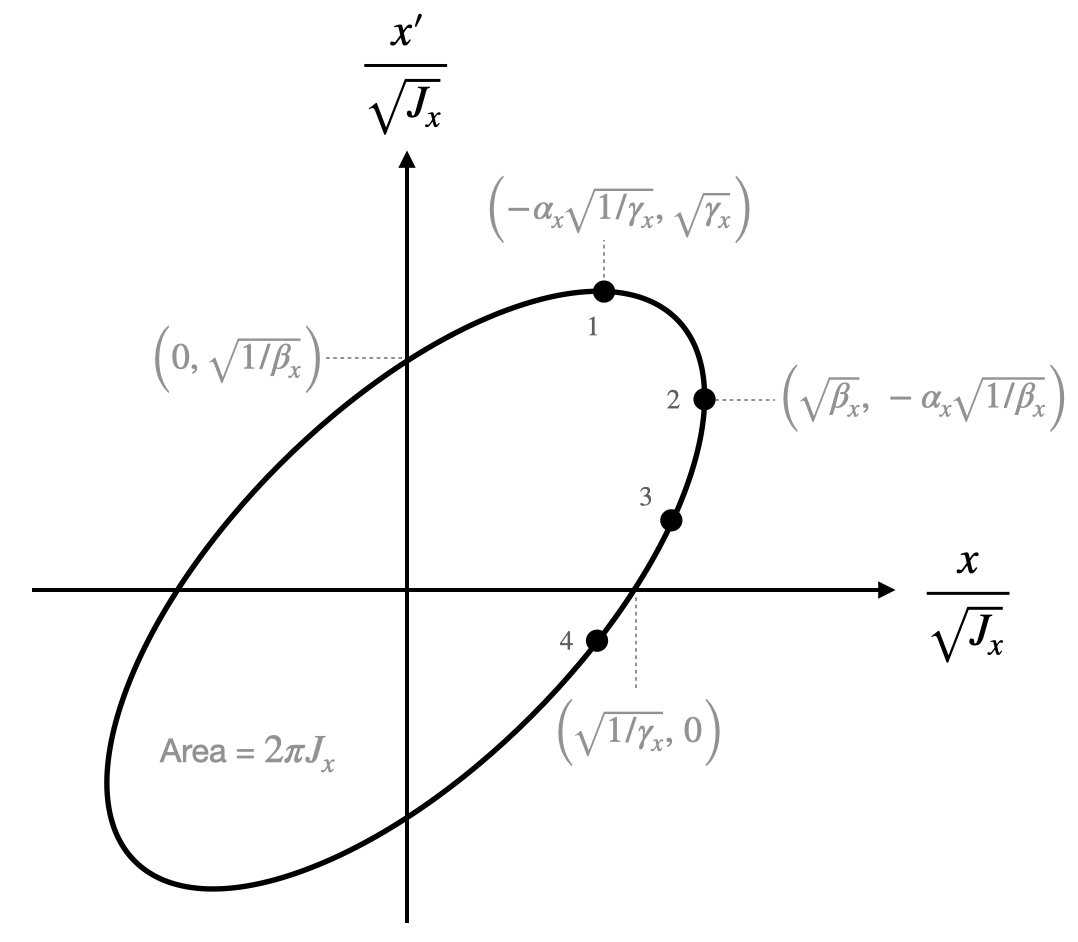
\includegraphics[width=0.6\textwidth]{Images/chapter1/cs_ellipse.png}
    \caption{Courant-Snyder ellipse in horizontal phase space.}
    \label{fig:cs_ellipse}
\end{figure}
%
The particle jumps around an ellipse. The so-called Twiss parameters $\beta$, $\alpha = -\beta' / 2$, and $\gamma = (1 + \alpha^2) / \beta$ determine the ellipse dimensions. $J$, which is proportional to the area of the ellipse, is called the Courant-Snyder invariant:
%
\begin{equation}\label{eq:CS invariant}
    J = \frac{x^2 + (\alpha x + \beta x')^2}{\beta}.
\end{equation}
%
We define the tune $\nu$ as the number of phase space oscillations per turn; i.e.,
%
\begin{equation}
    2\pi\nu = \oint{\frac{ds}{\beta(s)}},
\end{equation}
%
where the integral is around the entire ring.

Thus, motion between two locations in the ring is equivalent to an area-preserving linear transformation of a phase space ellipse, plus rotation of the particle around the ellipse. This is more clear in the transfer matrix formulation of the dynamics, writing $\mathbf{x}(s) = \mathbf{M}(s)\mathbf{x}(0)$ where
%
\begin{equation} \label{eq:CS_parameterization}
\begin{aligned}
    \mathbf{M}(s) &= 
    \begin{bmatrix} 
        \sqrt{\beta(s)} & 0 \\
        -\frac{\alpha(s)}{\sqrt{\beta(s)}} & \sqrt{\frac{1}{\beta(s)}}
    \end{bmatrix}
    \begin{bmatrix} 
        \cos\mu(s) & \sin\mu(s) 
        \\ -\sin\mu(s) & \cos\mu(s) 
    \end{bmatrix}
    \begin{bmatrix} 
        \sqrt{\frac{1}{\beta(0)}} & 0 \\
        \frac{\alpha(0)}{\sqrt{\beta(0)}} & \sqrt{\beta(0)}
    \end{bmatrix} \\
    &= \mathbf{V}(s) \, \mathbf{R}(s) \, \mathbf{V}(0)^{-1} 
\end{aligned}
\end{equation}
%
and $\mathbf{x} = (x, x')^T$. $\mathbf{V(0)}^{-1}$ transforms the phase space ellipse into a circle while preserving its area, $\mathbf{R(s)}$ rotates the coordinates around the circle according to the phase advance, and $\mathbf{V(s)}$ transforms the circle back into an ellipse \cite{Lee2011}. 

Eq.~\eqref{eq:CS_parameterization} motivates the definition of normalized phase space coordinates $\mathbf{x}_n(s) = \mathbf{V}(s)^{-1} \mathbf{x}(s)$ in which the particle performs simple harmonic oscillations; i.e., rotates in a circle of area $J$ at frequency $2\pi\nu$. 




\subsubsection{Linear (coupled) dynamics}

In the presence of linear coupling, the equations of motion take the following form:\footnote{I will occasionally switch between $\mathbf{x} = (x, x', y, y')^T$ and $\mathbf{x} = (x, y)^T$. The correct definition should be clear from context.}
%
\begin{equation}\label{eq:single_particle_eom_coupled}
    \mathbf{x}'' + \mathbf{K_0}(s) \mathbf{x} + \mathbf{K_1}(s) \mathbf{x}' = 0,
\end{equation}
%
where $\mathbf{x} = (x, y)^T$ and $\mathbf{K}_{0, 1}$ are $2 \times 2$ matrices. The particle now moves along an ellipsoid in 4D phase space ($x$-$x'$-$y$-$y'$), the volume of which is conserved. For example, Fig.~\ref{fig:skew_quad_single_particle_tbt} shows the turn-by-turn trajectory of a single particle in the presence of linear coupling from a rotated (skew) quadrupole.
%
\begin{figure}[!p]
    \centering
    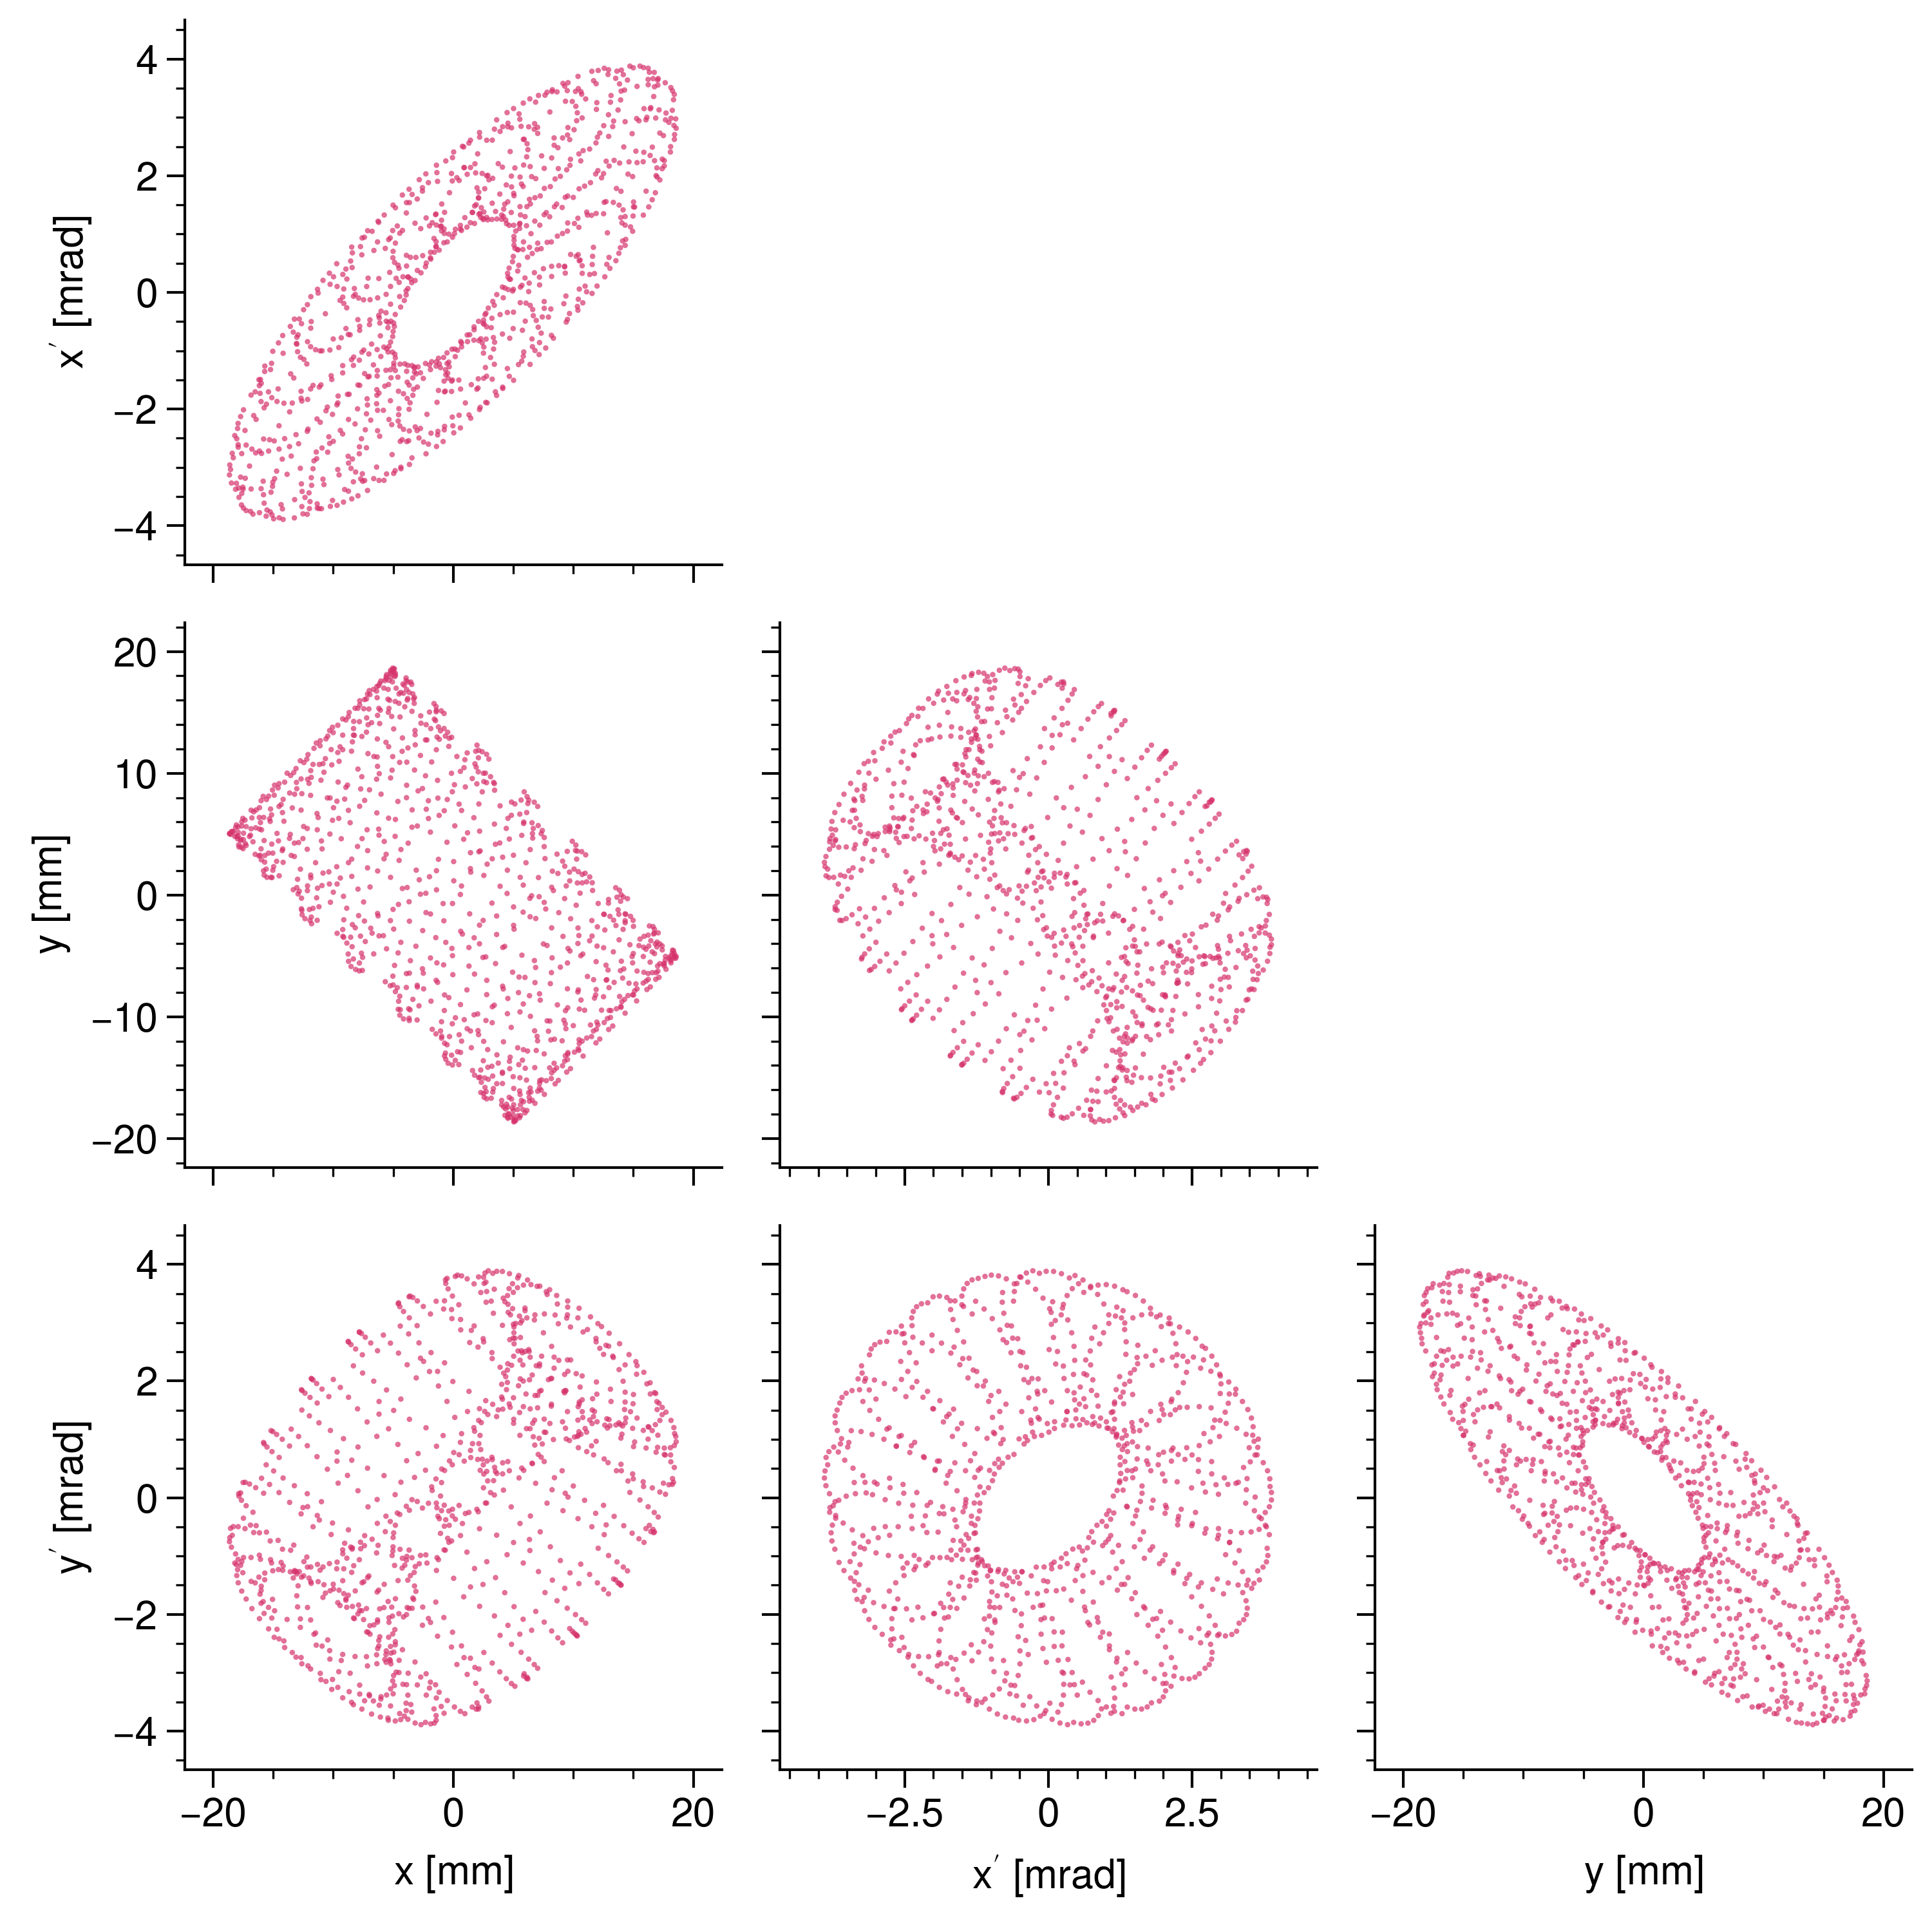
\includegraphics[width=0.85\textwidth]{Images/chapter1/skew_quad_single_particle_tbt.png}
    \caption{Turn-by-turn trajectory of a particle in a linear lattice with the addition of a skew quadrupole.}
    \label{fig:skew_quad_single_particle_tbt}
\end{figure}
%
The motion is most simply described using transfer matrices. Consider the eigenvectors and eigenvalues of the $4 \times 4$ symplectic one-turn transfer matrix $\mathbf{M}$. There are four eigenvectors — $\mathbf{v}_1$, $\mathbf{v}_2$, $\mathbf{v}_1^*$, $\mathbf{v}_2^*$ — and four eigenvalues — $\lambda_1$, $\lambda_2$, $\lambda_1^*$, $\lambda_2^*$ — with $\lambda_i\lambda_j^* = 1$ (* denotes the complex conjugate). The eigenvalue equation is written
%
\begin{equation} \label{eq:transfer_matrix_eig}
    \mathbf{M} \mathbf{v}_l = e^{-i\mu_l} \mathbf{v}_l,
\end{equation}
%
with $l = 1,2$. The phase space coordinate vector $\mathbf{x} = (x, x', y, y')^T$ at one position in the ring is a linear combination of the eigenvectors:
%
\begin{equation}
    \mathbf{x} = Re \left\{
        \sqrt{2 J_1} \, \mathbf{v}_1 \, e^{-i\psi_1}
        + \sqrt{2 J_2} \, \mathbf{v}_2 \, e^{-i\psi_2}
    \right\},
\end{equation}
%
where $J_{1,2}$ are constant amplitudes, $\psi_{1,2}$ are initial phases, and $Re\{z\}$ selects the real component of $z$. Application of the transfer matrix advances the phases:
%
\begin{equation}\label{eq:eigvec_coords}
    \mathbf{Mx} = Re \left\{
        \sqrt{2 J_1} \, \mathbf{v}_1 \, e^{-i(\psi_1 + \mu_1)}
        + \sqrt{2 J_2} \, \mathbf{v}_2 \, e^{-i(\psi_2 + \mu_2)}
    \right\}.
\end{equation}
%
The old invariants $J_{x,y}$ are replaced by $J_{1,2}$ and the phase advances $\mu_{x,y}$ are replaced by $\mu_{1,2}$. A new normalized phase space is defined by rewriting Eq.~\eqref{eq:eigvec_coords} as $\mathbf{x}_n = \mathbf{V}^{-1} \mathbf{x}$ with
%
\begin{equation}\label{eq:V_from_eigvecs}
    \mathbf{V} = 
    \begin{bmatrix}
        Re\{\mathbf{v}_1\}, & -Im\{\mathbf{v}_1\}, & Re\{\mathbf{v}_2\}, & -Im\{\mathbf{v}_2\}
    \end{bmatrix}.
\end{equation}
%
Particles perform simple harmonic oscillations in normalized phase space, moving in circles of area $J_1$ in the $x_n$-$x_n'$ plane and $J_2$ in the $y_n$-$y_n'$ plane.

We would like to parameterize the eigenvectors as in the uncoupled case. There are currently several parameterizations in existence \cite{Edwards1973, Ripken1989, Wolski2006, Lebedev2010, Qin2009}; we will use the parameterization of Lebedev and Bogacz \cite{Lebedev2010}:
%
\begingroup
\renewcommand*{\arraystretch}{1.5}
\begin{equation}
\begin{aligned}
    \mathbf{v}_1 = 
    \begin{bmatrix}
        \sqrt{\beta_{1x}} \\
        -\frac{\alpha_{1x} + i(1-u)}{\sqrt{\beta_{1x}}} \\
        \sqrt{\beta_{1y}}e^{i\nu_1} \\
        -\frac{\alpha_{1y} + iu}{\sqrt{\beta_{1y}}} e^{i\nu_1} \\
    \end{bmatrix} ,\quad
    \mathbf{v}_2 = 
    \begin{bmatrix}
        \sqrt{\beta_{2x}}e^{i\nu_2} \\
        -\frac{\alpha_{2x} + iu}{\sqrt{\beta_{2x}}}e^{i\nu_2} \\
        \sqrt{\beta_{2y}} \\
        -\frac{\alpha_{2y} + i(1-u)}{\sqrt{\beta_{2y}}} \\
    \end{bmatrix}.
\end{aligned}
\end{equation}
\endgroup
%
The meaning of the new parameters is illustrated in Fig.~\ref{fig:twiss4D}.
%
\begin{figure}[!p]
    \centering
    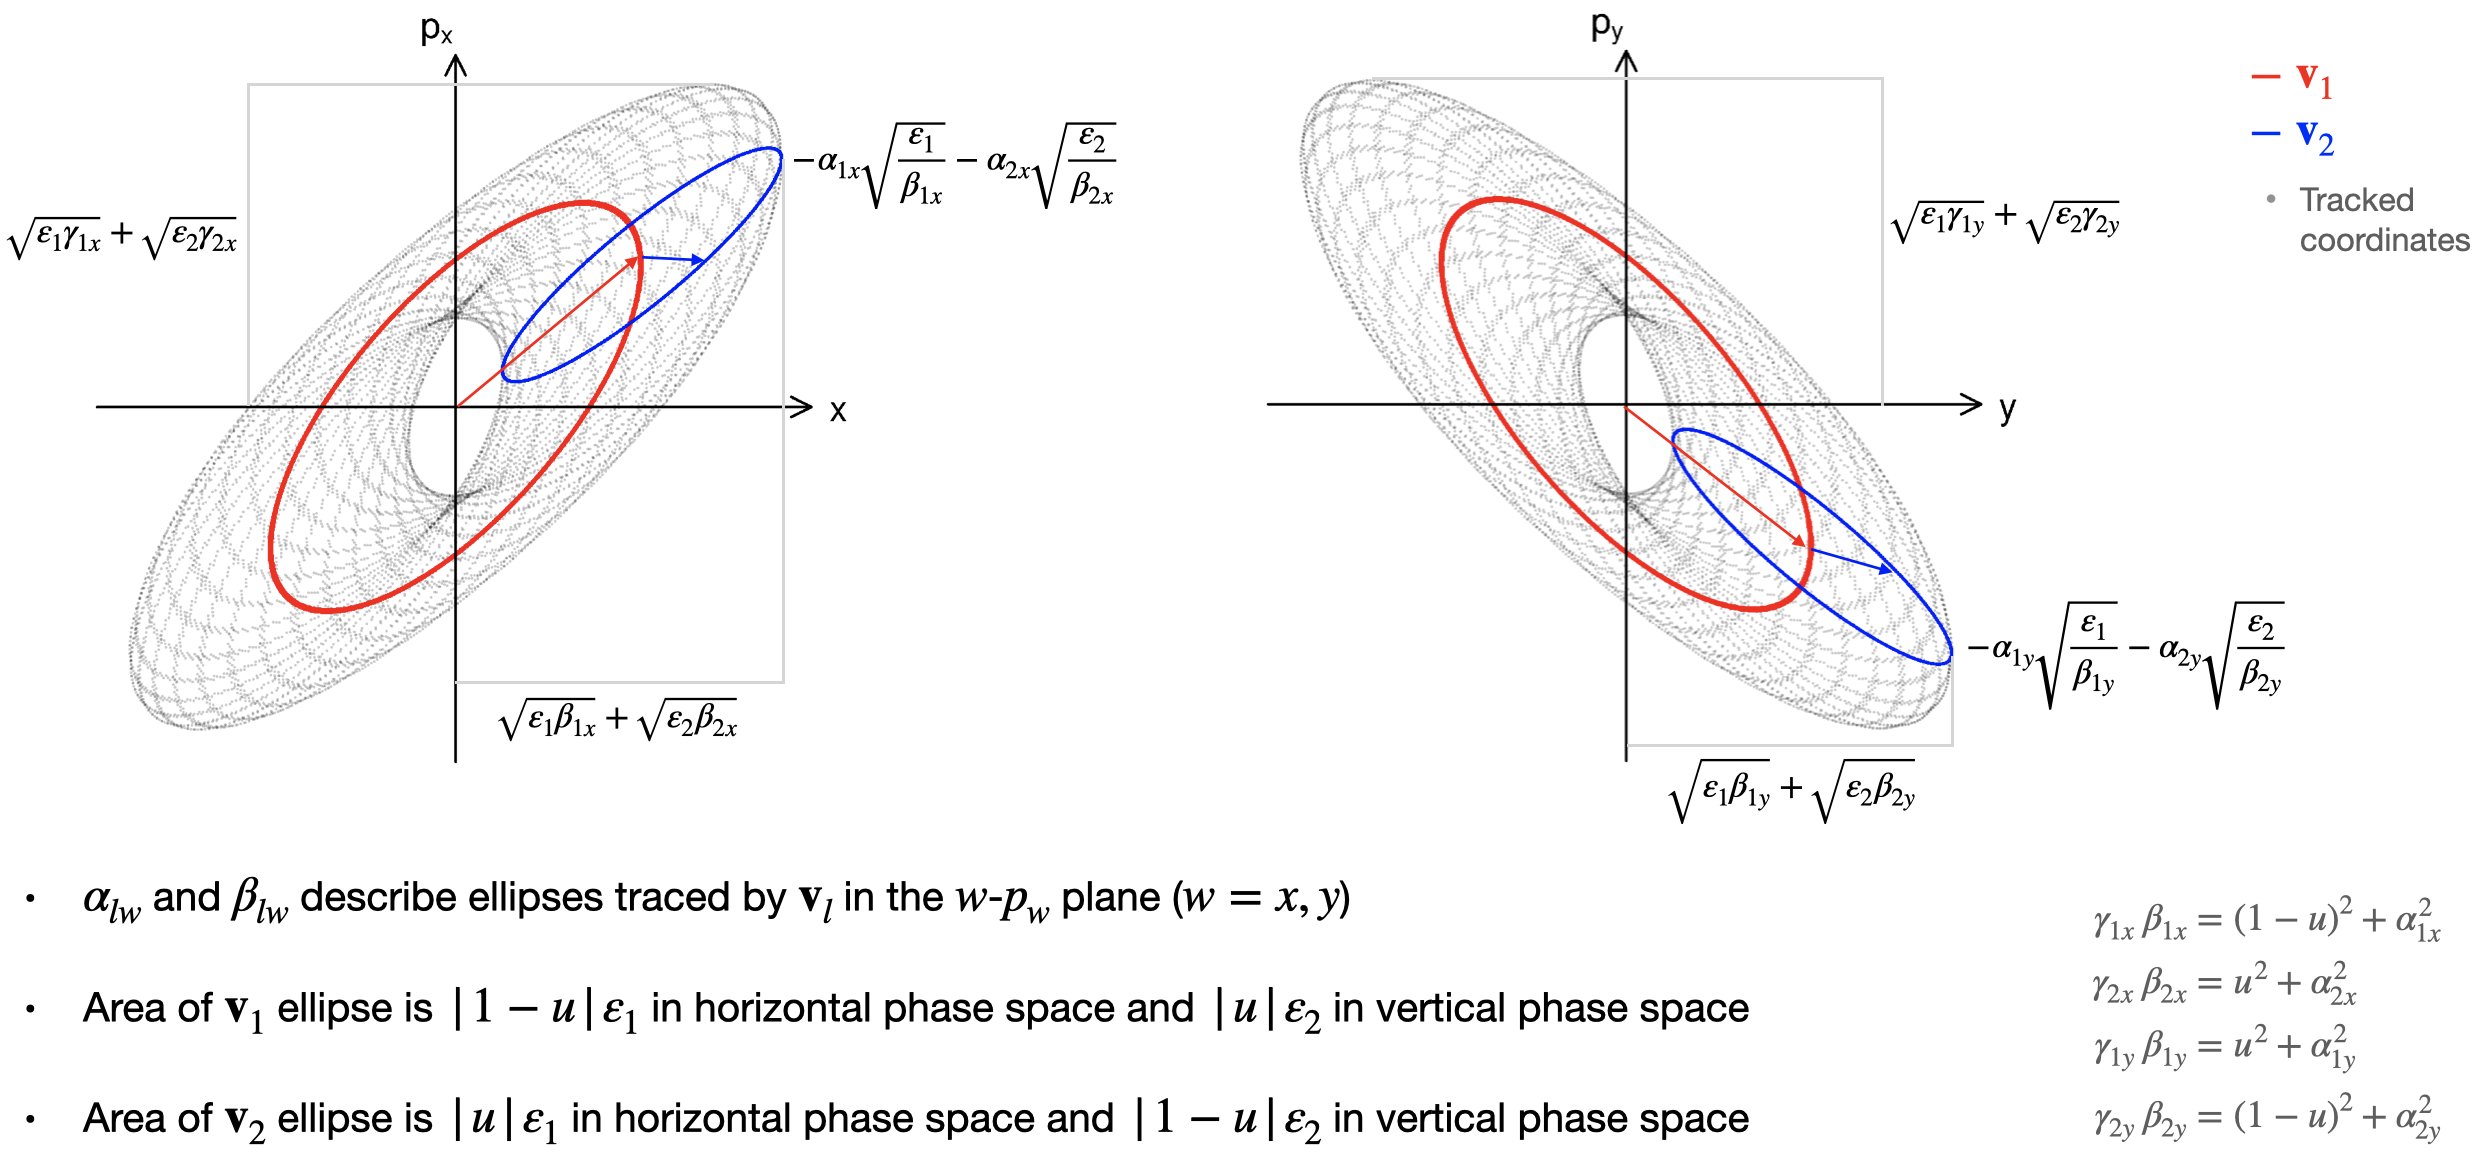
\includegraphics[width=\textwidth]{Images/chapter1/twiss4D.png}
    \vspace*{0.1cm}
    \caption{Lebedev-Bogacz parameterization of coupled motion. The grey markers are the turn-by-turn trajectory of a single particle. The red and blue lines are the ellipses traced by the transfer matrix eigenvectors.}
    \label{fig:twiss4D}
\end{figure}
%
The motion is the sum of two eigenvectors, each of which traces an ellipse when projected onto any 2D subspace. The frequency with which the ellipse is traced differs between the two modes; as a consequence, the horizontal and vertical amplitudes $J_x$ and $J_y$ are exchanged. The parameterization assigns a $\beta$ and $\alpha$ parameter to each ellipse. The parameters $\nu_1$ and $\nu_2$ are the phase differences between the horizontal ($x$-$x'$) and vertical ($y$-$y'$) parts of the eigenvectors, which determines the tilt angle of the ellipses traced in the cross-plane projections ($x$-$y$, $x$-$y'$, $y$-$x'$, $x'$-$y'$). Finally, $u$ determines the area of the ellipse traced by the eigenvectors in horizontal phase space relative to the ellipse in vertical phase space. 


\subsubsection{Nonlinear resonances}

Nonlinear terms in Eq.~\eqref{eq:magnetic_field_expansion} are generally small but nonzero in reality. Furthermore, they are periodic since they occur once per turn. As detailed in Appendix \ref{app-A}, perturbation analysis shows that these terms may drive a resonance when 
%
\begin{equation}\label{eq:resonance_lines}
    M_x \nu_x + M_y \nu_y = N,
\end{equation}
%
where $\nu_{x, y}$ are the single-particle tunes, $M_x$, $M_y$, and $N$ are integers, and $|M_x| + |M_y|$ is the order of the resonance. The single-particle tunes must be precisely controlled to avoid these resonance lines; otherwise, particles may be driven to large amplitudes and eventually fall outside the machine aperture. The strength of the resonance varies inversely with the order: fourth-order and below are the primary concern in most machines, but higher-order effects may be important when the number of stored turns is large. 



\subsection{Collective beam description}

A beam is a distribution of particles in phase space. In the limit of many particles, we define a distribution function $f(\mathbf{x})$ such that $f(\mathbf{x}) d\mathbf{x}$ gives the number of particles in an infinitesimal volume of phase space $d\mathbf{x}$. The measurable quantities are generally the projections of the distribution; e.g.
%
\begin{equation}
    f(x) = 
    \int_{-\infty}^{\infty}
    \int_{-\infty}^{\infty}
    \int_{-\infty}^{\infty}
    f(x, x', y, y') dx' dy dy'.
\end{equation}
%

It is often sufficient to characterize a distribution by its covariance matrix {$\bm{\Sigma} = \langle{\mathbf{x}\mathbf{x}^T}\rangle$}, where $\langle{\dots}\rangle$ represents the average over the distribution. In the transverse plane:
%
\begin{equation}\label{eq:covariance_matrix}
\begin{aligned}
    \bm{\Sigma} &= 
    \begin{bmatrix}
        \langle{xx}\rangle & \langle{xx'}\rangle & \langle{xy}\rangle & \langle{xy'}\rangle \\
        \langle{xx'}\rangle & \langle{x'x'}\rangle & \langle{x'y}\rangle & \langle{x'y'}\rangle \\
        \langle{xy}\rangle & \langle{x'y}\rangle & \langle{yy}\rangle & \langle{yy'}\rangle \\
        \langle{xy'}\rangle & \langle{x'y'}\rangle & \langle{yy'}\rangle & \langle{y'y'}\rangle 
    \end{bmatrix}
    &= 
    \begin{bmatrix}
        \bm{\sigma}_{xx} & \bm{\sigma}_{xy} \\
        \bm{\sigma}^T_{xy} & \bm{\sigma}_{yy}
    \end{bmatrix}.
\end{aligned}
\end{equation}
%
If a linear transformation $\mathbf{x} \rightarrow \mathbf{M}\mathbf{x}$ is applied to the coordinates, the covariance matrix transforms as
%
\begin{equation}\label{covariance_matrix_transport}
    \bm{\Sigma} 
    \rightarrow 
    \mathbf{M} \, \bm{\Sigma} \, \mathbf{M}^T.
\end{equation}
%
The covariance matrix defines an ellipsoid in phase space: $\mathbf{x}^T \bm{\Sigma}^{-1} \mathbf{x} = 1$. The 4D emittance $\varepsilon_{4D}$ is proportional to the volume of this ellipsoid:
%
\begin{equation} 
    \varepsilon_{4D} = \left|{\bm{\Sigma}}\right|^{1/2}
\end{equation}
%
where $|...|$ is the determinant. The 4D emittance is conserved under any linear transformation. The horizontal and vertical emittances $\varepsilon_{x,y}$ are individually conserved if the transformation is uncoupled:
%
\begin{equation}
\begin{aligned}
    \varepsilon_x = \left|{\bm\sigma}_{xx}\right|^{1/2}, \quad
    \varepsilon_y = \left|{\bm\sigma}_{yy}\right|^{1/2}
\end{aligned}
\end{equation}
%
These correspond to the areas in the $x$-$x'$ and $y$-$y'$ planes. 

In the absence of cross-plane correlations ($\bm{\sigma}_{xy} = 0$), the 4D emittance is equal to the product of the horizontal and vertical emittances, which are referred to as the \textit{apparent} emittances from now on. Instead, the 4D emittance is the product of the \textit{intrinsic} emittances $\varepsilon_1$ and $\varepsilon_2$:
%
\begin{equation} \label{eq:mode_emittances1}
    \varepsilon_{4D} = \left|{\bm{\Sigma}}\right|^{1/2} = \varepsilon_1\varepsilon_2 \le \varepsilon_x\varepsilon_y.
\end{equation}
%
The intrinsic emittances are found by a symplectic diagonalization of $\bm{\Sigma}$, i.e., they are the imaginary components of the eigenvalues of $\bm{\Sigma}\mathbf{U}$, where $\mathbf{U}$ is the unit symplectic matrix:
%
\begin{equation}
    \mathbf{U} = 
    \begin{bmatrix}
        0 & 1 & 0 & 0 \\
        -1 & 0 & 0 & 0 \\
        0 & 0 & 0 & 1 \\
        0 & 0 & -1 & 0
    \end{bmatrix}.
\end{equation}
%
The answer can be written compactly \cite{Xiao2013}:
%
\begin{equation}
    \varepsilon_{1, 2} = \frac{1}{2}\sqrt{
      -tr\left[(\bm{\Sigma} \mathbf{U})^2\right] \pm \sqrt{tr^2\left[(\bm{\Sigma} \mathbf{U})^2\right] - 16|{\bm{\Sigma}}|},
    }
\end{equation}
%
The intrinsic emittances are individually conserved in any linear focusing system. Their product is less than or equal to the product of the apparent emittances \cite{Buon1993}.

It is challenging to generate initial distributions for simulations \cite{Lund2009}. A simple strategy is to assume elliptical symmetry and construct a distribution from the single-particle invariants $J_{x,y}$.\footnote{Alternatively, the generalized invariants $J_{1, 2}$ can be used.} We define the ellipsoid parameter $T = {J_x}/{\varepsilon_x} + {J_y}/{\varepsilon_y}$ and stack ellipsoids to create the distribution, writing $f = f(T)$. One option is a Gaussian distribution: $f_{gauss} \propto \exp(-T/2)$. Another is the Waterbag distribution, which is a uniformly filled ellipsoid: $f_{wb} \propto \Theta(1 - T)$, where $\Theta$ is the Heaviside step function. Another is the KV distribution, which is a uniformly populated ellipsoidal shell: $f_{kv} \propto \delta(1 - T)$. The 1D and 2D projections of these 4D distributions are shown in Fig.~\ref{fig:distributions_gaussian}, Fig.~\ref{fig:distributions_waterbag}, and Fig.~\ref{fig:distributions_kv}. The black ellipse shows the covariance matrix ellipsoid projected onto the planes, multiplied by a factor of four. Since the distributions share the same covariance matrix, they are said to be rms-equivalent.
%
\begin{figure}[!p]
    \begin{subfigure}{0.49\textwidth}
        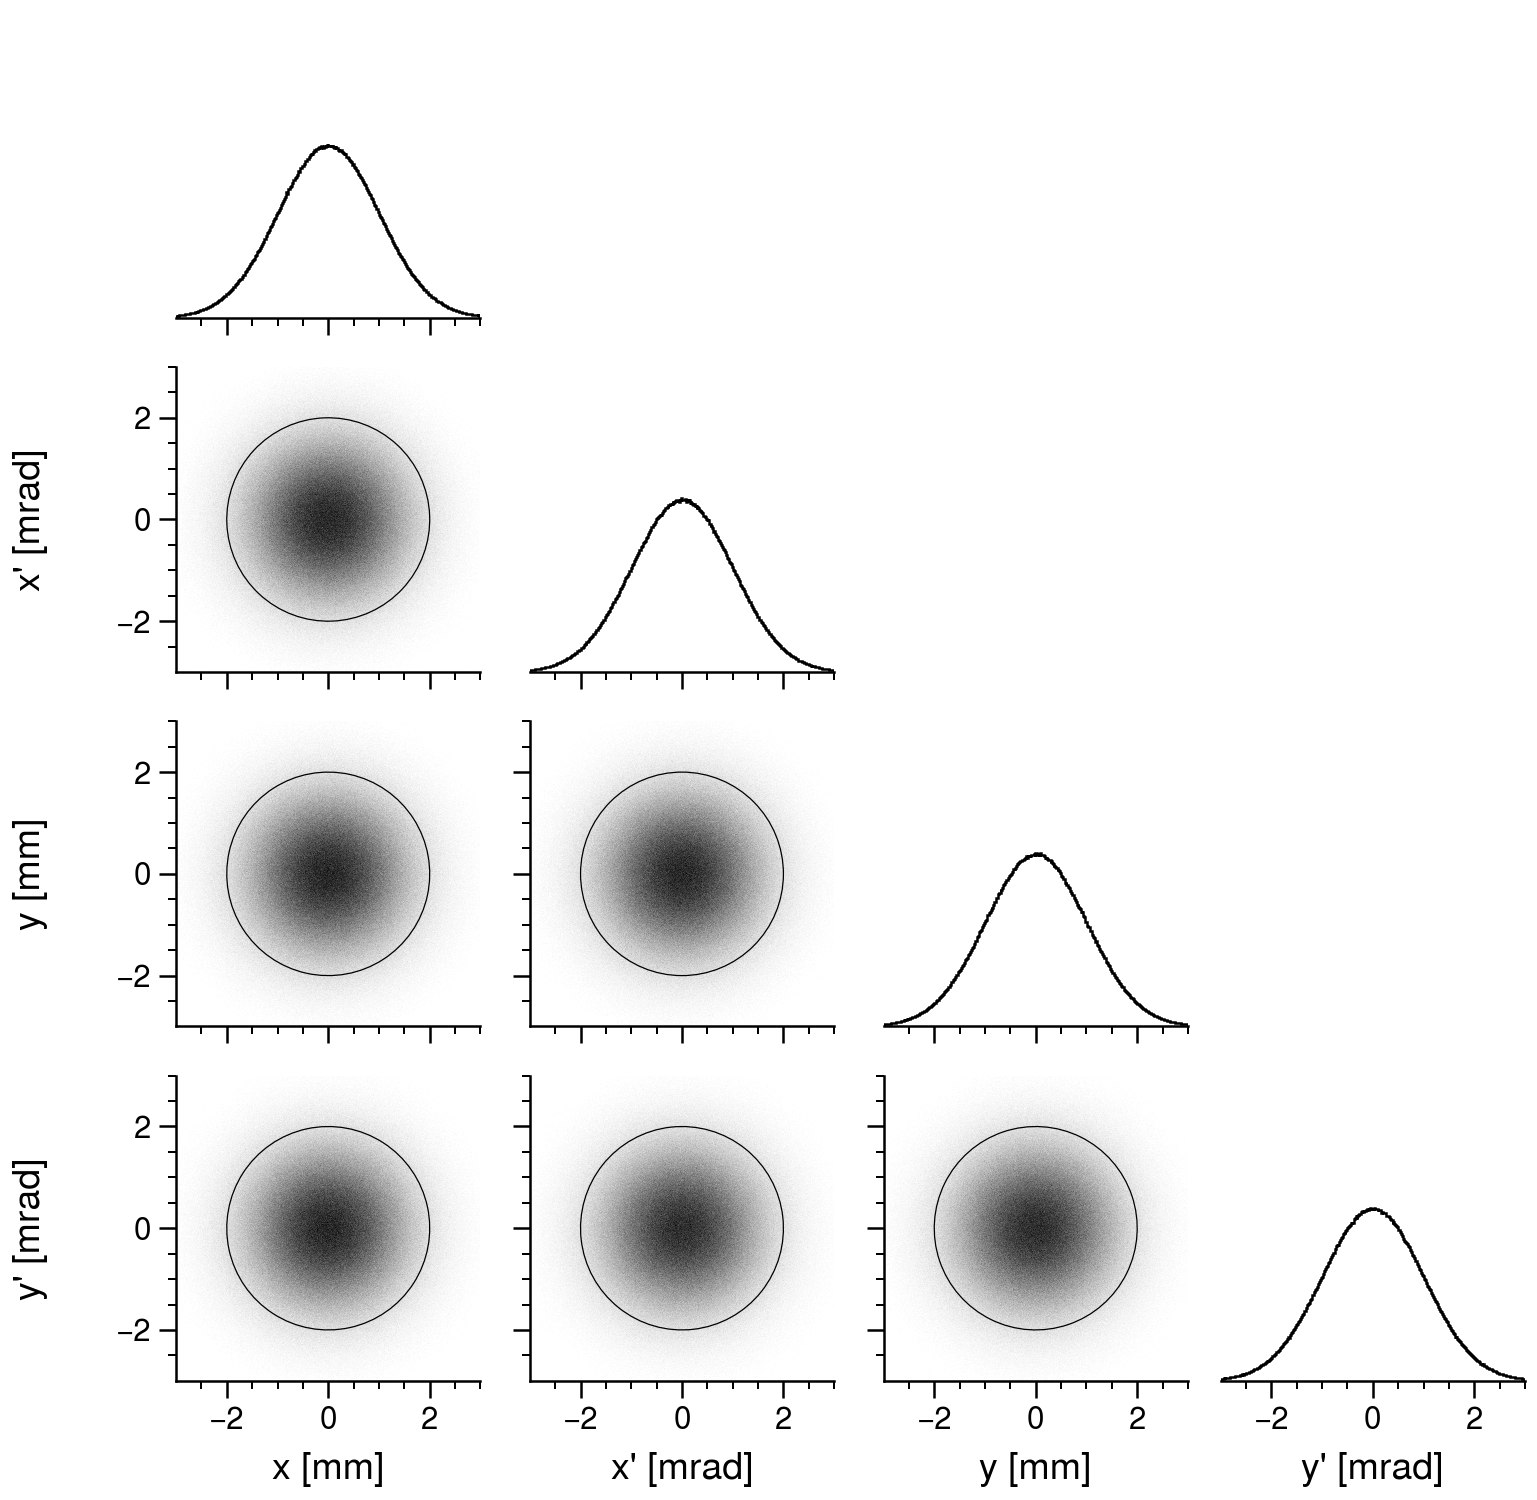
\includegraphics[width=\textwidth]{Images/chapter1/Gaussian_dist.png}
        \caption{Gaussian distribution}
        \label{fig:distributions_gaussian}
    \end{subfigure}
    \hfill
    \begin{subfigure}{0.49\textwidth}
        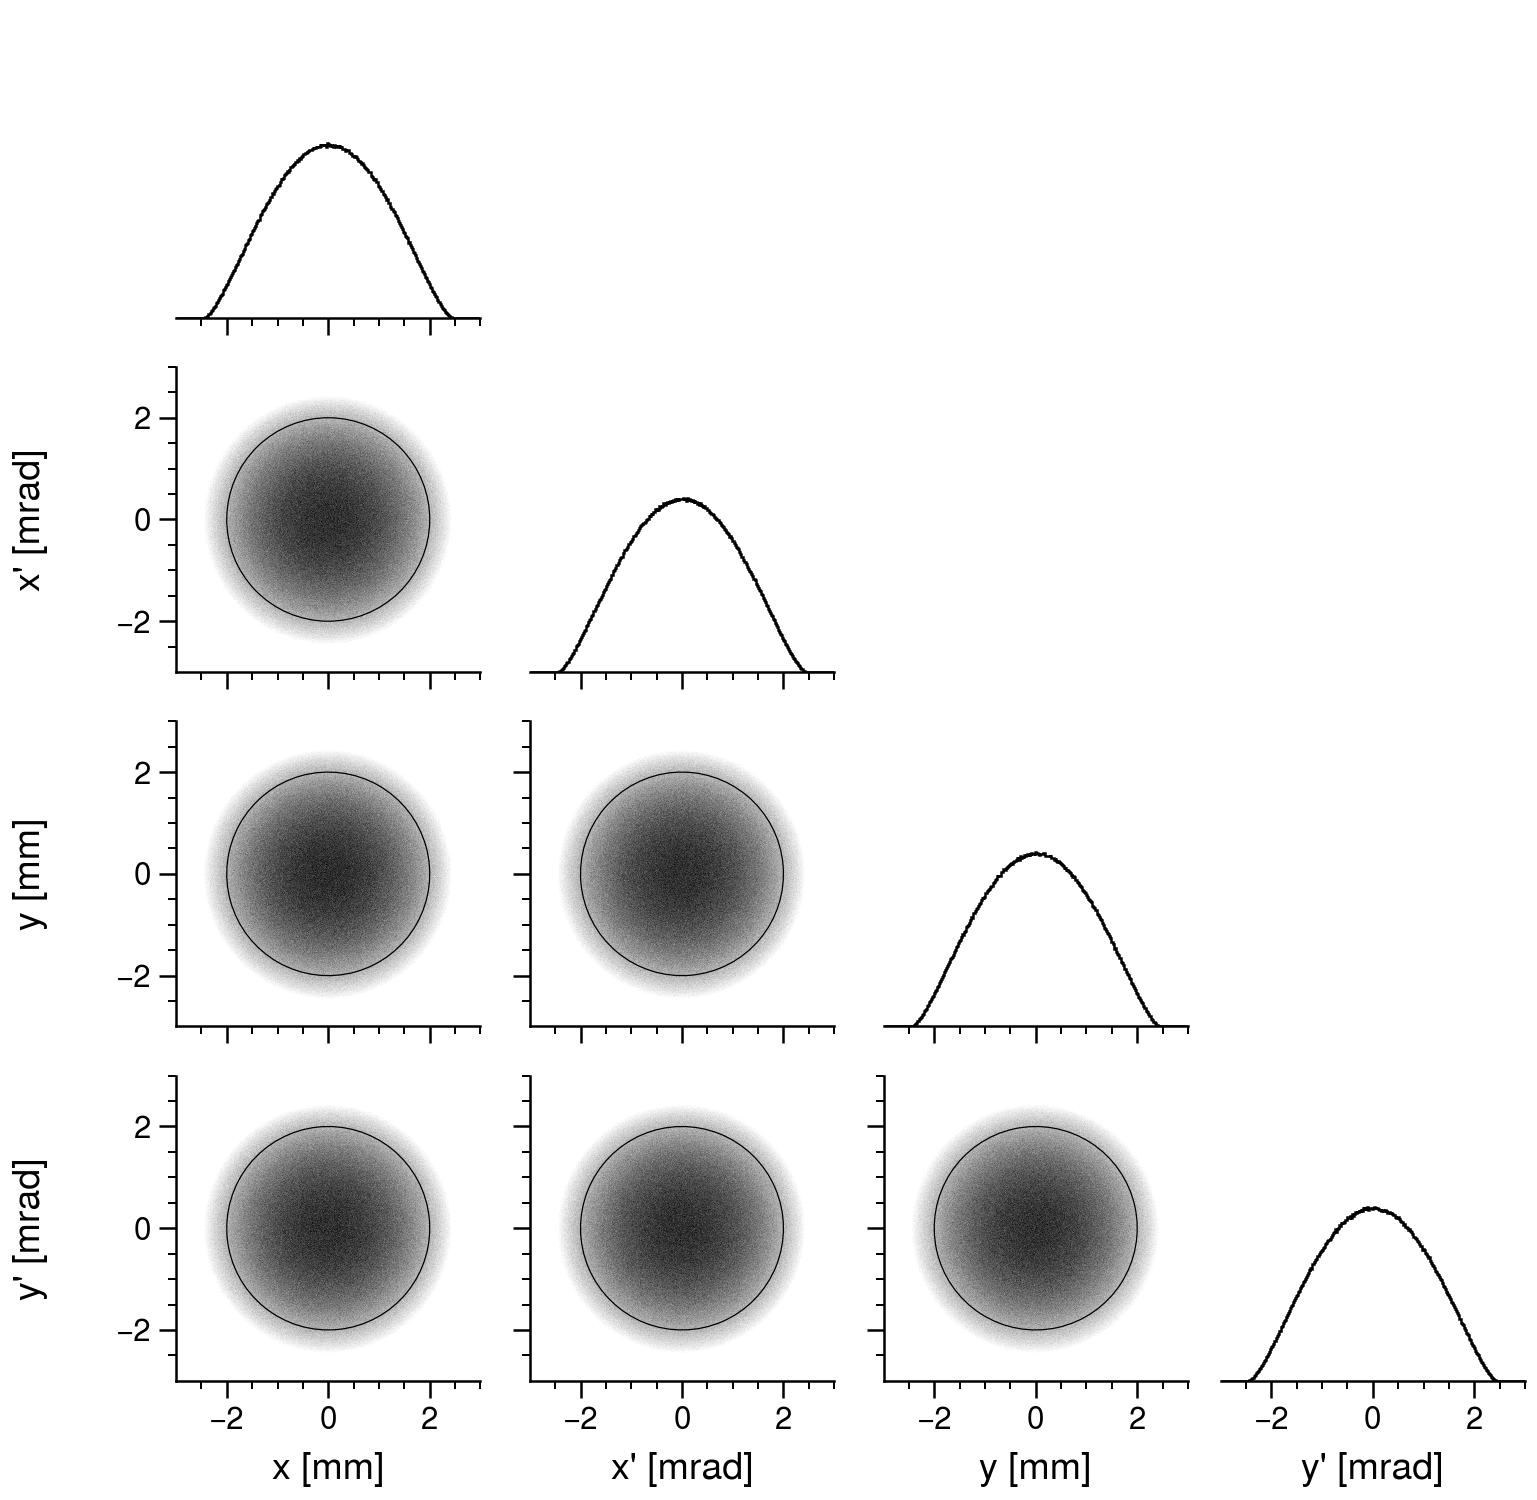
\includegraphics[width=\textwidth]{Images/chapter1/Waterbag_dist.png}
        \caption{Waterbag distribution}
        \label{fig:distributions_waterbag}
    \end{subfigure}
    \vfill
    \begin{subfigure}{0.49\textwidth}
        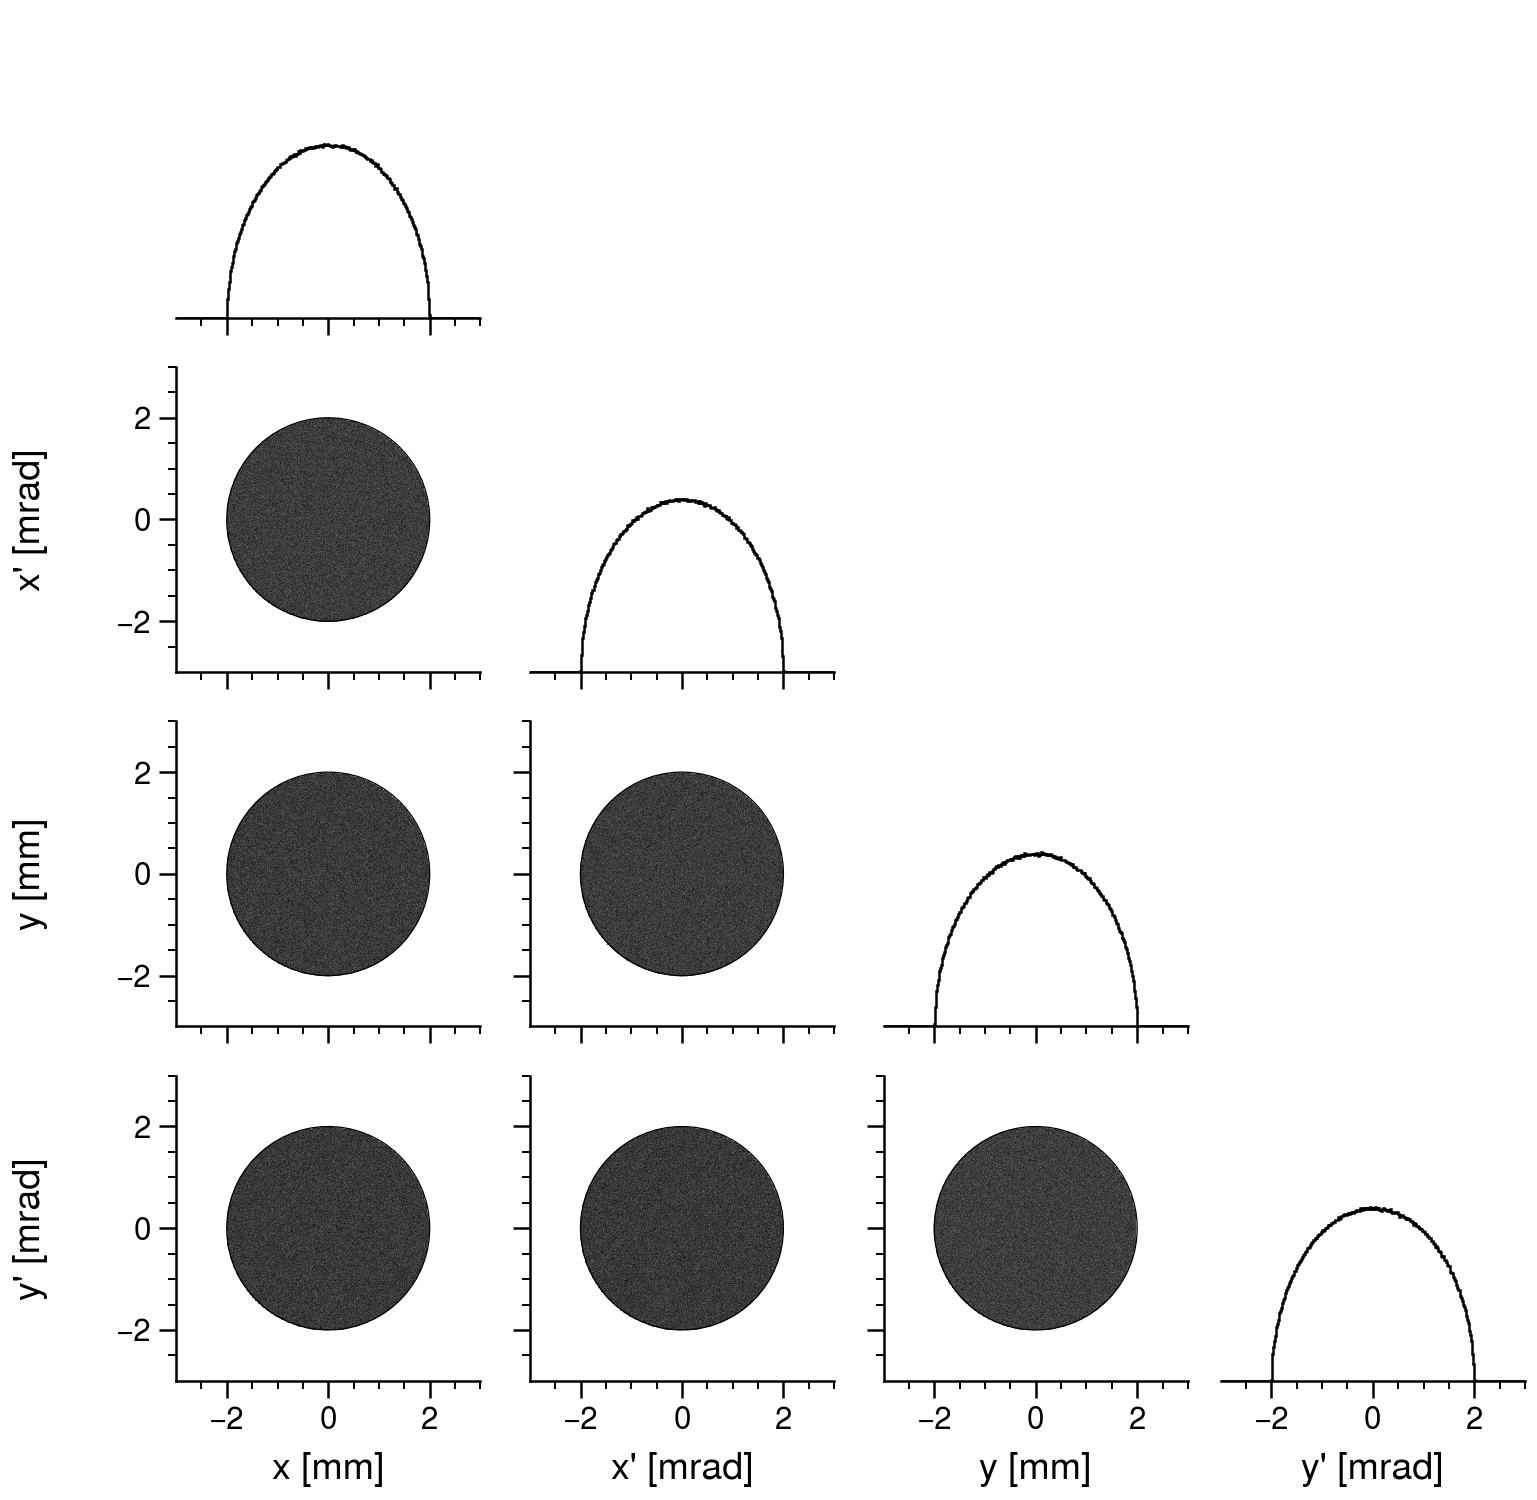
\includegraphics[width=\textwidth]{Images/chapter1/KV_dist.png}
        \caption{KV distribution}
        \label{fig:distributions_kv}
    \end{subfigure}
    \hfill
    \begin{subfigure}{0.49\textwidth}
        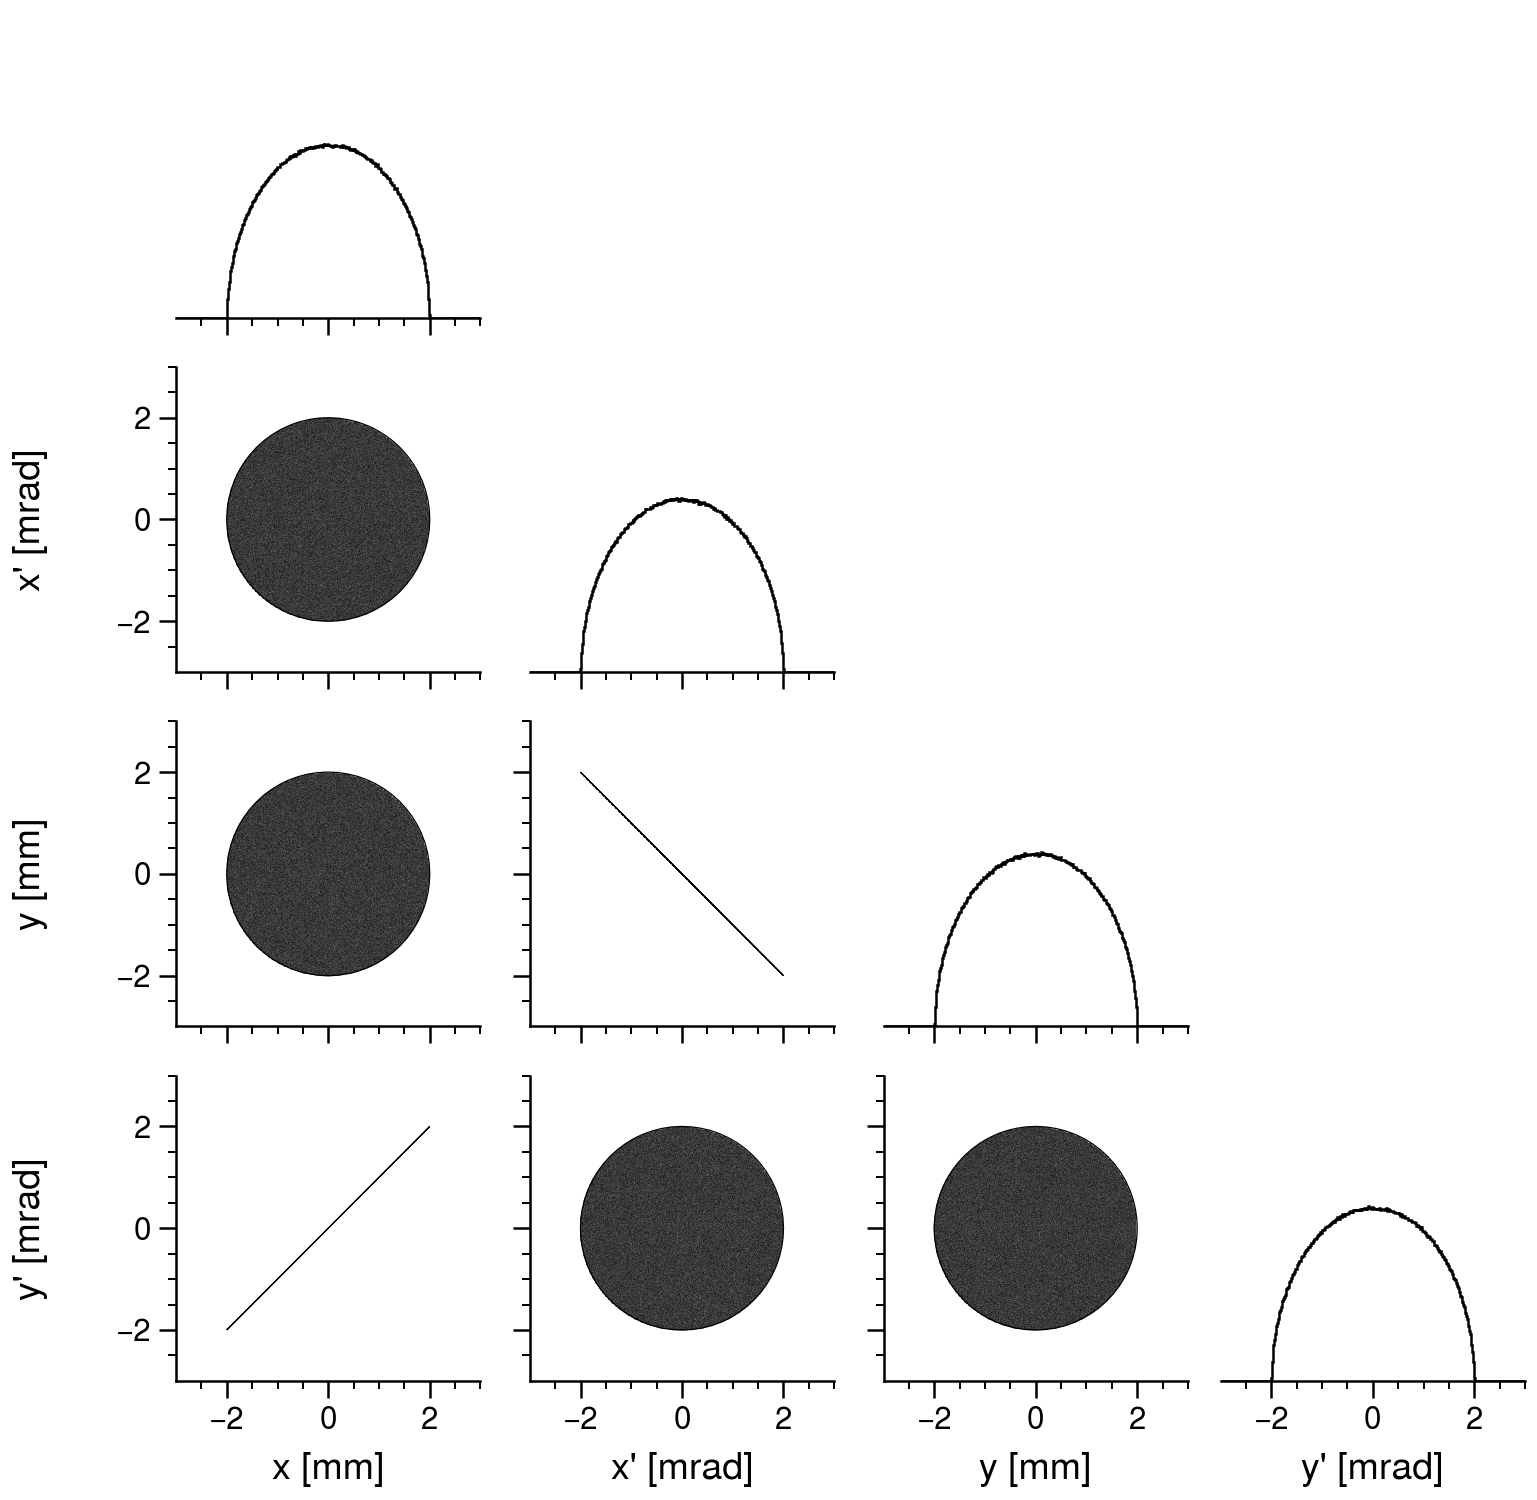
\includegraphics[width=\textwidth]{Images/chapter1/Danilov_dist.png}
        \caption{Danilov distribution}
        \label{fig:distributions_danilov}
    \end{subfigure}
    \caption{1D and 2D projections of various 4D phase space distributions. Black ellipses are defined by four times the distribution covariance matrix.}
    \label{fig:distributions}
\end{figure}
%






\subsection{Space charge}\label{sec:Space charge}

Particle motion is also influenced by the beam space charge — the charge density of the beam in free space. The beam electric field $\mathbf{E} = (E_x, E_y)$ modifies the single-particle equation of motion:
%
\begin{equation}\label{eq:eom_with_spacecharge}
    \mathbf{x}'' + \mathbf{K_0}(s) \mathbf{x} + \mathbf{K_1}(s) \mathbf{x}' = \frac{q}{m\gamma_s^3\beta_s^2c^2} \mathbf{E},
\end{equation}
% 
Due to the attractive magnetic force between co-moving charges in the lab frame, the space charge force approaches zero as $\beta_s \rightarrow 1$. We will make the coasting beam approximation — infinite length, uniform density, and constant momentum in the longitudinal plane — to reduce the problem to two dimensions.\footnote{This is generally invalid for linacs but locally valid for a transverse slice of a long distribution in a ring. It is equivalent to replacing particles with infinitely long uniform density charged rods.}

Following Hofmann \cite{Hofmann2017Book}, we divide space charge effects into two categories: incoherent effects involving the motion of single particles, and coherent effects involving the self-consistent motion of the entire beam. Although the two effects may be difficult to isolate during the beam evolution \cite{Hofmann2021}, the distinction is clear in some cases. 


\subsubsection{Incoherent effects}

We first assume that the beam is matched — i.e., oscillates with the same periodicity as the external focusing — and track a particle in the field of the matched beam. This may be justified if space charge is weak. If the beam's electric field is linear in the transverse coordinates, it will simply modify the external linear focusing; therefore, the single-particle tune is reduced in both planes. A primary concern in rings is that the depressed tunes are located near one of the low-order resonance lines in Fig.~\ref{fig:resonance_lines}. Approximate analytical formulas for the tune shift can be obtained \cite{Ng2005} but are not presented here.

If the electric field is nonlinear, the tune shift will depend on the particle amplitude, leading to a spread of tunes. An intuitive explanation is that large-amplitude particles experience a weaker average electric field throughout one turn in the ring \cite{Franchetti2017}. A recent study of the space charge tune spread in rings is found in \cite{Hotchi2020}. Fig.~\ref{fig:jparc_montague}, taken from the paper, shows the simulated tune spread in the Japan Proton Accelerator Research Center (J-PARC).
%
\begin{figure}[!p]
    \centering
    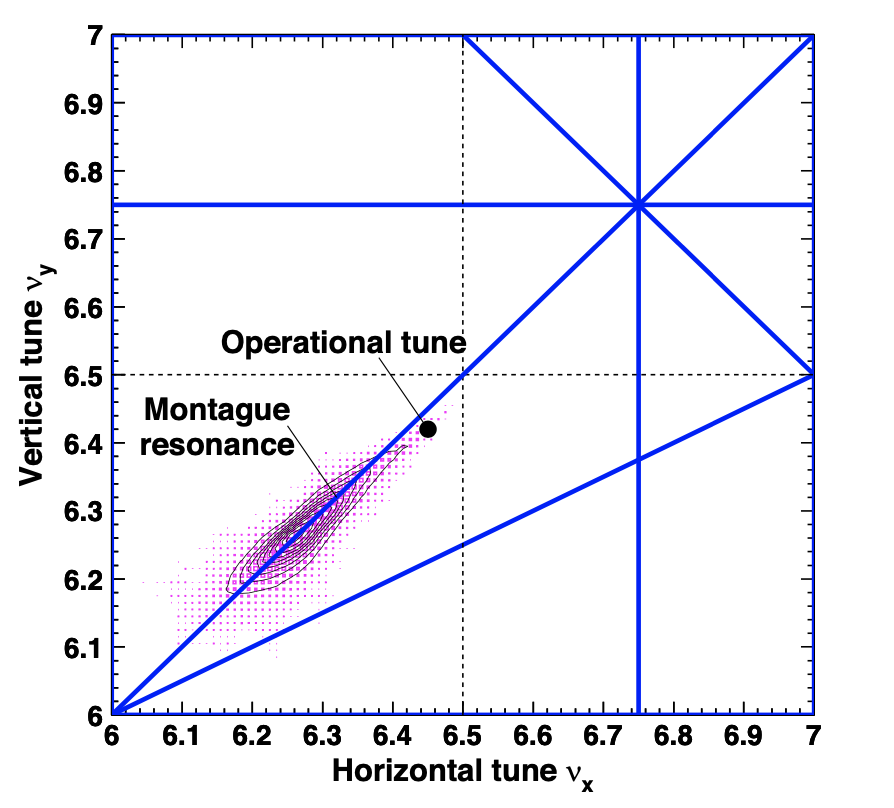
\includegraphics[width=0.6\textwidth]{Images/chapter1/montague.png}
    \caption{Simulated tune footprint in the JPARC accelerator. (From \cite{Hotchi2020})}
    \label{fig:jparc_montague}
\end{figure}
%

Thus, the beam intensity in a ring is fundamentally limited by the incoherent space charge tune shift. A rough guideline is that the maximum tune shift should be kept below 0.25 to avoid fourth-order resonance lines \cite{book:Reiser}, but specific requirements depend on the application. Note that, as described in Appendix \ref{app-B}, it is also possible for the beam's electric field to drive single-particle resonances in this model.



\subsubsection{Coherent effects}

Coherent space charge effects involve self-consistent oscillations of the entire beam \cite{book:Reiser, Wangler2008, Cousineau2003}. We may model the beam as a smooth distribution in phase space $f(\mathbf{x}, \mathbf{x}', s)$; neglecting collisions between particles, the evolution of $f$ is given by the Vlasov equation \cite{Vlasov1961}:
%
\begin{equation} \label{eq:Vlasov}
    \frac{d}{ds}{f(\mathbf{x}, \mathbf{x}', s)} = 
    \frac{\partial{f}}{\partial{s}} +
    \mathbf{x}' \cdot \frac{\partial{f}}{\partial{\mathbf{x}}} +
    \mathbf{x}'' \cdot \frac{\partial{f}}{\partial{\mathbf{x'}}}
    = 0,
\end{equation}
%
Hidden in Eq.~\eqref{eq:Vlasov} is the single-particle equation of motion, which we rewrite as:
%
\begin{equation}
    \mathbf{x}'' + \mathbf{K_0} \mathbf{x} + \mathbf{K_1} \mathbf{x}'
    =
    \frac{q}{m\gamma_s^3\beta_s^2c^2} \frac{\partial{\Phi}}{\partial\mathbf{x}},
\end{equation}
%
with the space charge potential $\Phi$ determined from the Poisson equation:
%
\begin{equation} \label{eq:Poisson}
    \frac{\partial^2{\Phi}}{\partial{\mathbf{x}^2}} = -\frac{q}{\epsilon_0}
    \int_{-\infty}^{\infty}{f}d\mathbf{x}'.
\end{equation}
%

Analysis of the Vlasov equation is difficult in the general case of time-dependent external forces; thus, computer simulation must be used to understand the beam evolution. Solutions exist, but are rare (see Section \ref{sec:Self-consistent phase space distributions}). Perturbations of the Vlasov equation around these solutions can be used to derive stability conditions for the coherent oscillations of the beam, albeit this is only feasible in simple cases. This idea is explored in Appendix \ref{app-B}. 




\section{Self-consistent phase space distributions}\label{sec:Self-consistent phase space distributions}

\subsection{Definition and properties}

Any function constructed from single-particle invariants $\{C_i\}$ is a solution of the Vlasov equation:
%
\begin{equation}\label{eq:vlasov_equilibria}
    \frac{d}{ds} f(\{C_i\}) = \sum_{i}{\frac{df}{dC_i}\frac{dC_i}{ds}} = 0.
\end{equation}
%
One example of a single-particle invariant when the focusing is linear and time-dependent is the Courant-Snyder invariant of Eq.~\eqref{eq:CS invariant}. The inclusion of space charge complicates the identification of invariants, and the only known solutions are those that produce linear space charge forces. We label such distributions as \textit{self-consistent}: a self-consistent distribution produces linear space charge forces, and the linearity of the space charge force is conserved under any linear transformation \cite{Danilov2003}. 

Self-consistent distributions possess several notable properties. First, the integro-differential system of equations in Eq.~\eqref{eq:Vlasov} is reduced to a system of ordinary differential equations. Second, nonlinear space charge effects are minimized: the emittance is conserved, the maximum space charge tune shift is minimized, and the space charge tune spread is eliminated. Third, higher-order coherent instabilities may be present in self-consistent distributions due to their small tune spread. Fourth, known self-consistent distributions have a uniform charge density.



\subsection{Known solutions}

Danilov et al. enumerated a class of self-consistent distributions in $2d$-dimensional phase space \cite{Danilov2003}: 
%
\begin{equation}\label{eq:scdist_general_form}
    f\left({\mathbf{x}, \mathbf{x}'}\right) = 
    g\left({H - H_b}\right)
    \prod_{i=1}^{m}\delta\left({\mathbf{e}_i \cdot \mathbf{x} 
    + \mathbf{e}'_i \cdot \mathbf{x}'}\right),
\end{equation}
%
where $\mathbf{x}$, $\mathbf{x}'$ are the $d$ dimensional vector coordinates and momenta, $g$ is a function of $H$ — a quadratic positively defined function of the phase space coordinates — and $H_b$ — an upper bound on $H$ — $\delta$ is the Dirac delta function, and $\mathbf{e}_i$, $\mathbf{e}'_i$ are vectors of constants. This is referred to as the $\{n,m\}$ case. It was proven that the electric field within any uniformly filled ellipsoid is linear, and that any distribution of the form of $\eqref{eq:scdist_general_form}$ that produces a linear electric field will do so under any linear transformation.

In other words, one class of self-consistent distributions consists of those that generate linear space charge forces and are constructed from quantities that are invariant in the presence of linear focusing. We now focus on the \{2, 0\} and \{2, 2\} cases. (Qin and Davidson derived a self-consistent distribution for $n = 2$ in \cite{Qin2013} using their recent parameterization of coupled motion, but made no reference to \cite{Danilov2003}. The connection between Danilov's work and Qin and Davidson's work should be explored in the future.)


\subsubsection{The KV distribution}

The $\{2, 0\}$ case corresponds to the KV distribution derived by Kapchinskij and Vladimirskij in 1959 \cite{Kapchinskij1959}. The distribution is a function of the Courant-Snyder invariants $J_x$ and $J_y$:
%
\begin{equation}
    f(\mathbf{x}, \mathbf{x}') = \frac{\lambda}{\pi^2 \varepsilon_x\varepsilon_y}
    \delta \left(\frac{J_x}{\varepsilon_x} + \frac{J_y}{\varepsilon_y} -1 \right),
\end{equation}
%
where $\lambda$ is the longitudinal particle density. Particles in the KV distribution are evenly distributed on an ellipsoidal shell in 4D phase space. As shown in Fig.~\ref{fig:distributions_kv}, any 2D projection of the distribution is a uniform density ellipse. Of particular importance is the $x$-$y$ projection, which remains upright and uniform density under any uncoupled transformation. The electric field within such an ellipse is
%
\begin{equation}  \label{eq:field_in_upright_ellipse}
    \mathbf{E}(x, y) =
    \frac{\lambda}{\pi\epsilon_0}
    \left[ 
        \frac{x}{c_x\left(c_x+c_y\right)} \hat{x}
        + \frac{y}{c_y\left(c_x+c_y\right)} \hat{y}
    \right],
\end{equation}
%
where $c_x$ and $c_y$ are the horizontal and vertical semi-axes and $\epsilon_0$ is the permittivity of free space. Since the space charge force is linear and uncoupled, $J_{x,y}$ remains invariant for every particle and the emittances $\varepsilon_{x,y}$ are conserved. The KV distribution does not exist in three spatial dimensions \cite{Sacherer1968}.

As mentioned in the previous section, the preservation of the linearity of the space charge force leads to a self-consistent set of differential equations for the evolution of the beam envelope. The KV envelope equations read:
%
\begin{align} \label{eq:KV_envelope}
    \tilde{x}'' + k_{x}(s)\tilde{x} - \frac{\varepsilon_x^2}{\tilde{x}^3} - \frac{Q}{2\left(\tilde{x} + \tilde{y}\right)} &= 0, \\
    \tilde{y}'' + k_{y}(s)\tilde{y} - \frac{\varepsilon_y^2}{\tilde{y}^3} - \frac{Q}{2\left(\tilde{x} + \tilde{y}\right)} &= 0. \nonumber
\end{align}
%
The RMS widths of the beam $\tilde{x} = \sqrt{\langle{{x^2}}\rangle}$ and $\tilde{y} = \sqrt{\langle{{y^2}}\rangle}$ are used instead of the true widths $c_x$ and $c_y$. They are related by a factor of two for a uniform density ellipse. The perveance $Q$ is a dimensionless measure of space charge strength:
%
\begin{equation}\label{eq:perveance}
    Q = \frac{2\lambda r_0}{\beta^2\gamma^3},
\end{equation}
%
where $r_0 = e^2 / 4\pi\epsilon_0mc^2$ is the classical proton radius. Eqs.~\eqref{eq:KV_envelope} provide many insights into dynamical beam behavior and serve as a benchmark for computer simulations.  

A remarkable fact is that Eqs.~\eqref{eq:KV_envelope} are exact for distributions with elliptical symmetry even if the space charge force is nonlinear \cite{Sacherer1968}. They are not closed, however, since the emittances would then depend on time. Thus, the KV envelope equations provide a good approximation to the evolution of more realistic distributions in the limit of elliptical symmetry and small emittance growth \cite{Lund2004}.


\subsubsection{The Danilov distribution}

The focus of this dissertation is on the $\{2, 2\}$ case of Eq.~\eqref{eq:scdist_general_form} which will be referred to as the Danilov distribution:
%
\begin{equation}
    f(\mathbf{x}, \mathbf{x}') \propto 
    \Theta\left({1 - \mathbf{x}^T\bm{\mathbf{\sigma}^{-1}}\mathbf{x}}\right)
    \delta\left({\mathbf{x} - \mathbf{D}\mathbf{x}'}\right)
\end{equation}
%
with 
%
\begin{equation}
    \bm{\sigma} = 
    4
    \begin{bmatrix}
        \langle{xx}\rangle & \langle{xy}\rangle \\
        \langle{xy}\rangle & \langle{yy}\rangle
    \end{bmatrix}
\end{equation}
%
and $\mathbf{D}$ a $2 \times 2$ matrix. Similar to the KV distribution, any 2D projection of the Danilov distribution is a uniform density ellipse; however, the ellipses in the cross-plane projections ($x$-$y$, $x$-$y'$, $y$-$x'$, $x'$-$y'$) are not necessarily upright and may collapse to lines. For example, the projections are shown in Fig.~\ref{fig:distributions_danilov} for $\mathbf{D}_{11}=\mathbf{D}_{22}=0$ and $\mathbf{D}_{12} = -\mathbf{D}_{21}=1$, which corresponds to a rigidly rotating disk. The electric field in a uniform density ellipse with semi-axes $c_{x,y}$ tilted at an angle $\phi$ in the $x$-$y$ plane is:
%
\begin{equation}
\begin{aligned}
    E_x &\propto 
    \left({\frac{\cos^2\phi}{c_x} + \frac{\sin^2\phi}{c_y}}\right) \frac{x}{c_x + c_y}
    +
    \sin\phi\cos\phi \left({\frac{1}{c_y} - \frac{1}{c_x}}\right) \frac{y}{c_x + c_y}, \\
    E_y &\propto 
    \left({\frac{\cos^2\phi}{c_y} + \frac{\sin^2\phi}{c_x}}\right) \frac{y}{c_x + c_y}
    +
    \sin\phi\cos\phi \left({\frac{1}{c_y} - \frac{1}{c_x} }\right) \frac{x}{c_x + c_y}.
\end{aligned}
\end{equation}
%
The field is linear in $x$ and $y$, as required. And it is worth repeating: the linearity of the electric field is maintained under any linear transformation. The key difference from the KV distribution is that space charge linearly couples the horizontal and vertical motion of individual particles. The Courant-Snyder invariants $J_{x,y}$ are therefore replaced by the more general invariants $J_{1, 2}$, which are conserved even with the inclusion of space charge. 

The delta functions in the Danilov distribution function cause the four-dimensional emittance, and therefore one of the intrinsic emittances, to be zero. The following relationship has been found to hold:
%
\begin{equation} \label{eq:mode_emittances2}
    \varepsilon_1 = \varepsilon_x + \varepsilon_y, \quad
    \varepsilon_2 = 0
\end{equation}
%
or vice versa. 

Discussion of the Danilov envelope equations is reserved for Chapter \ref{chap-2}.




\section{Producing a self-consistent distribution}\label{sec:Producing a self-consistent distribution}


\subsection{Motivation}

The following points motivate the physical realization of a self-consistent distribution.

\begin{enumerate}
\item 
The properties listed in section~\ref{sec:Self-consistent phase space distributions} — conservation of emittance, reduced space charge tune shift, and reduced space charge tune spread — have the potential to increase the maximum intensity in a ring.

\item
It is an interesting challenge to bring a real distribution closer to a self-consistent analytical model which is generally taken to be unrealistic. 

\item
Beams with a uniform charge density are ideal for fixed-target applications such as spallation neutron production. SNS targets are complex and expensive \cite{Haines2014} and considerable research and development goes into reducing the peak density on the target. This issue will become even more important if future machines are built on the intensity horizon with similar targets.

\item
There has been recent interest in generating circular modes, where a circular mode is a beam with small 4D emittance. Such a beam can be transformed to a round state ($\varepsilon_x = \varepsilon_y$) or a flat state ($\varepsilon_x \ll \varepsilon_y$) using coupled linear optics that preserve $\varepsilon_{1,2}$. In \cite{Burov2002}, several potential applications of circular modes are listed. Consider first a round-flat transformation. The fractional increase in beam luminosity, a figure of merit in colliders, in this case is
%
\begin{equation}
    C = \sqrt{\frac{\varepsilon_x\varepsilon_y}{\varepsilon_1\varepsilon_2}},
\end{equation}
%
which approaches $\infty$ as $\varepsilon_1\varepsilon_2 \rightarrow 0$. Flat beams may also increase the possible beam intensity in a ring by suppressing incoherent space charge resonances in one dimension, freeing large areas of tune space. The possible uses of flat beams in the Large Hadron Collider (LHC) are suggested by Burov in \cite{Burov2013}. Alternatively, round beams may be helpful for the suppression of beam-beam effects at collider interaction points \cite{Danilo1996}. Circular modes may also find use in relativistic electron cooling \cite{Burov2000}, low-energy hadron cooling \cite{Derbenev2000}, muon ionization cooling, and radiation generation \cite{Corlett2001}. The connection between the Danilov distribution and circular modes is straightforward: the Danilov distribution is a circular mode with uniform charge density. This connection is illustrated in Fig.~\ref{fig:circular_modes_diagram}.
%
\begin{figure}[!p]
    \centering
    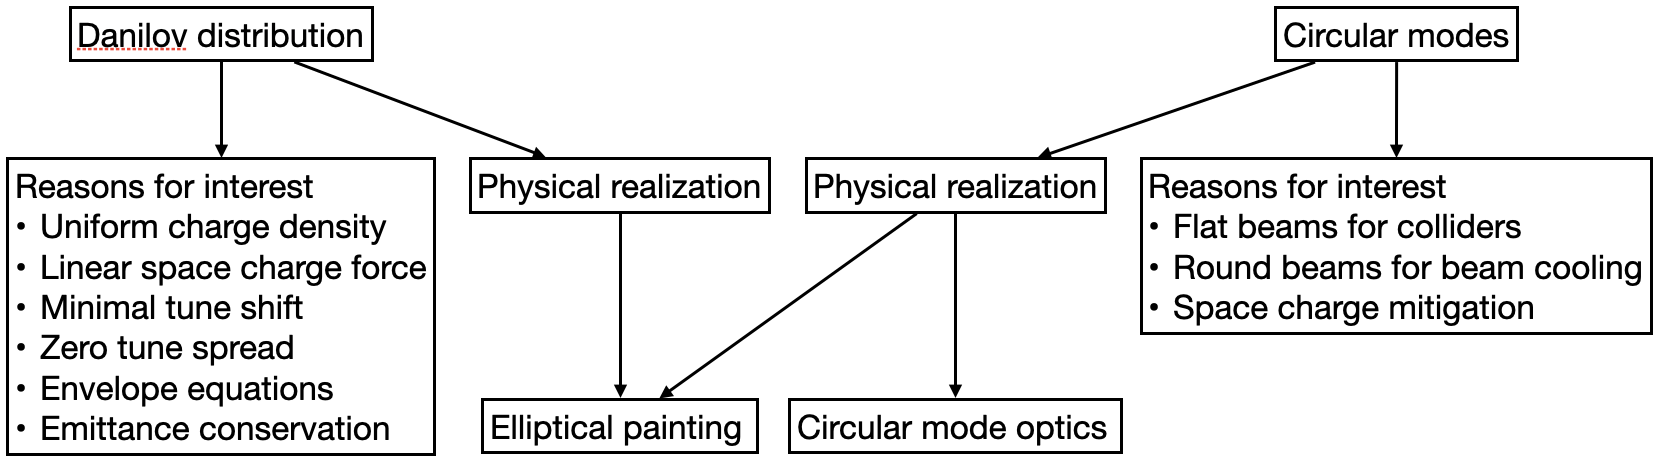
\includegraphics[width=\textwidth]{Images/chapter1/diagram.png}
    \caption{Connection between circular modes, the Danilov distribution, and the elliptical painting method.}
    \label{fig:circular_modes_diagram}
\end{figure}
%

\end{enumerate}

\subsection{Previous experimental work}

Luiten et al. proposed a method to create a \{3, 3\} distribution (a 3D uniform density ellipsoid) of electrons \cite{Luiten2004}. They observed that since a uniform density oblate spheroid\footnote{$(x/A)^2 + (y/B)^2 + (z/C)^2 = 1$ with $A = B > C$} will collapse under its own gravity into a flat disk \cite{Lin1965}, a flat transverse disk of electrons will longitudinally expand into a uniform density ellipsoid. This ``pancake" distribution can be created using ultrashort pulsed-laser photoemission with an appropriate radial intensity profile. Musumeci et al. experimentally demonstrated this method in \cite{Musumeci2008}. Their measurements are shown in Fig.~\ref{fig:Musumeci}.
%
\begin{figure}[!p]
    \centering
    % \begin{subfigure}{0.75\textwidth}
    %     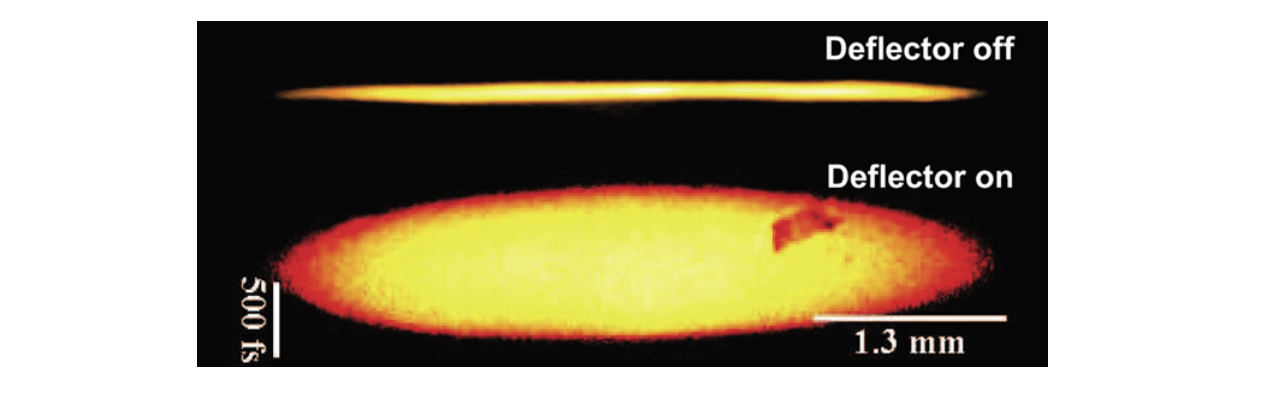
\includegraphics[width=\textwidth]{Images/chapter1/Musumeci_fig2.png}
    %     \label{fig:Musumeci_a}
    %     \caption{}
    % \end{subfigure}
    % \vfill
    % \vspace*{1.5cm}
    % \vfill
    % \begin{subfigure}{0.75\textwidth}
    %     \centering
    %     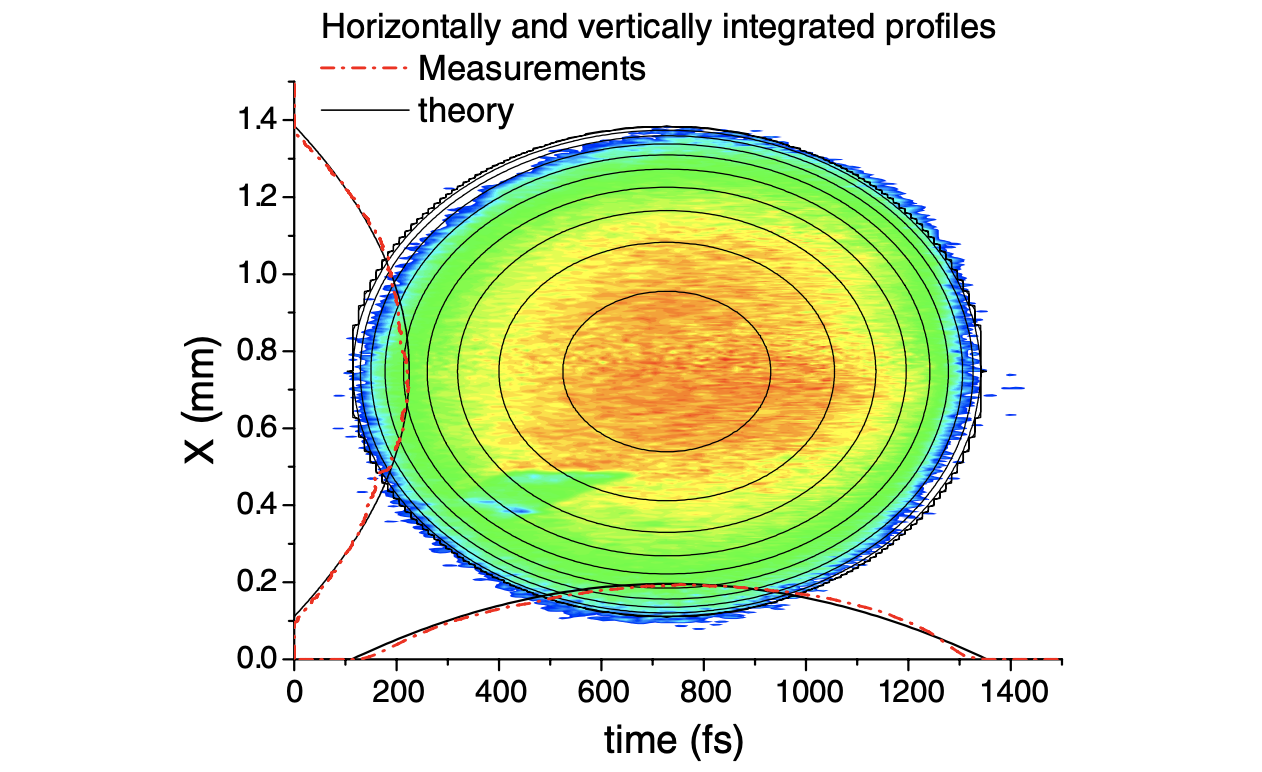
\includegraphics[width=\textwidth]{Images/chapter1/Musumeci_fig3.png}
    %     \label{fig:Musumeci_b}
    %     \caption{Lower image in (a), displayed with a different color map, and 1D projections of the image.}
    % \end{subfigure}
    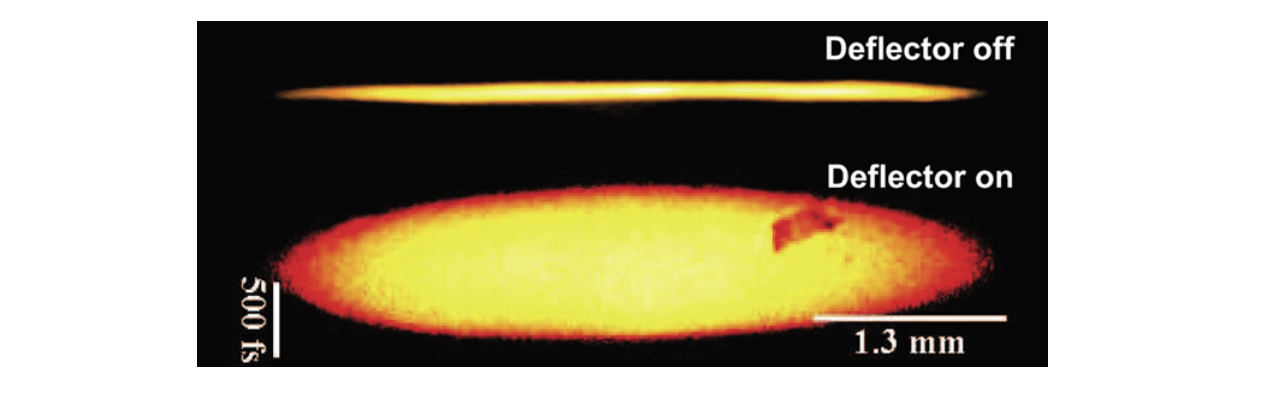
\includegraphics[width=0.85\textwidth]{Images/chapter1/Musumeci_fig2.png}
    \caption{Measured electron beam in the $x$-$z$ plane from \cite{Musumeci2008}.}
    \label{fig:Musumeci}
\end{figure}
%

Unfortunately, these methods do not apply to high-intensity proton rings where distributions are much longer, often resembling 2D coasting beams, and are built up over many turns. The rest of this section describes a method to generate a Danilov distribution in a high-intensity proton ring using the concept of phase space painting, as well as the implementation of the method in the SNS.


\subsection{Phase space painting}

Accelerators are often broken into stages. A common pattern is the injection of a beam from a linac into a ring followed by eventual extraction to a different section of the machine. Injection and extraction are accomplished using kicker magnets — dipole magnets with fast rise times.

In direct multi-turn injection, multiple beam pulses are injected into the same stable region of longitudinal phase space in the ring. This process is limited by Liouville's theorem in the sense that the phase space density in the ring cannot be increased. In charge-exchange injection, an ion beam from the linac is stripped of its electrons upon entering the ring, leaving only protons.\footnote{Electrons are currently stripped using foils. Laser stripping is a potential alternative \cite{Cousineau2017}.} This produces a higher phase space density because charge-exchange is a non-Liouvillian process. While normal multi-turn injection is usually performed over tens of turns, charge-exchange injection is performed over hundreds of turns \cite{Bracco2017}.\footnote{There is, however, renewed interest in direct multi-turn injection for future accelerators to avoid the issues associated with charge exchange injection, such as foil scattering and unstripped particles, and it seems possible to extend the number of injected turns into the hundreds using novel injection schemes \cite{Prior2016}.} 

Phase space painting, or simply ``painting", is the time-dependent variation of the transverse distance and angle between the injected beam and the circulating beam; as such, it allows time-dependent control over the phase space distribution in the ring. Painting is a vital tool for space charge mitigation. The free parameters are the painting path — the path of the injection point in phase space — and the speed at which this path is traversed. After discussing the two most popular painting methods, we will introduce a new method called elliptical painting that theoretically produces a Danilov distribution.


\subsection{Square root painting methods}

Although particles move along elliptical trajectories in $x$-$x'$ and $y$-$y'$ phase space in the linear approximation, they explore a rectangular region in the $x$-$y$ plane due to differences in the horizontal and vertical tunes. Square root painting methods make the best of this situation by theoretically generating uniform density ellipses in $x$-$x'$ and $y$-$y'$ phase space. 

\subsubsection{Correlated painting}

Let $x$, $x'$, $y$, and $y'$ be the coordinates of the injected beam in the phase space of the circulating beam, and $t$ be a time variable normalized to the range [0, 1]. In its simplest form, correlated painting proceeds as
%
\begin{equation}
\begin{aligned}
    {x}(t) &= {x}_{max}\sqrt{t}, \\
    {y}(t) &= {y}_{max}\sqrt{t}, \\
    x'(t) &= y'(t) = 0.
\end{aligned}
\end{equation}
%
In the linear approximation and without space charge, correlated painting generates uniform density ellipses in the $x$-$x'$ and $y$-$y'$ planes and a rectangular distribution in the $x$-$y$ plane. This is illustrated on the left side of Fig.~\ref{fig:painting_graphic}. 
%
\begin{figure}[!p]
    \centering
    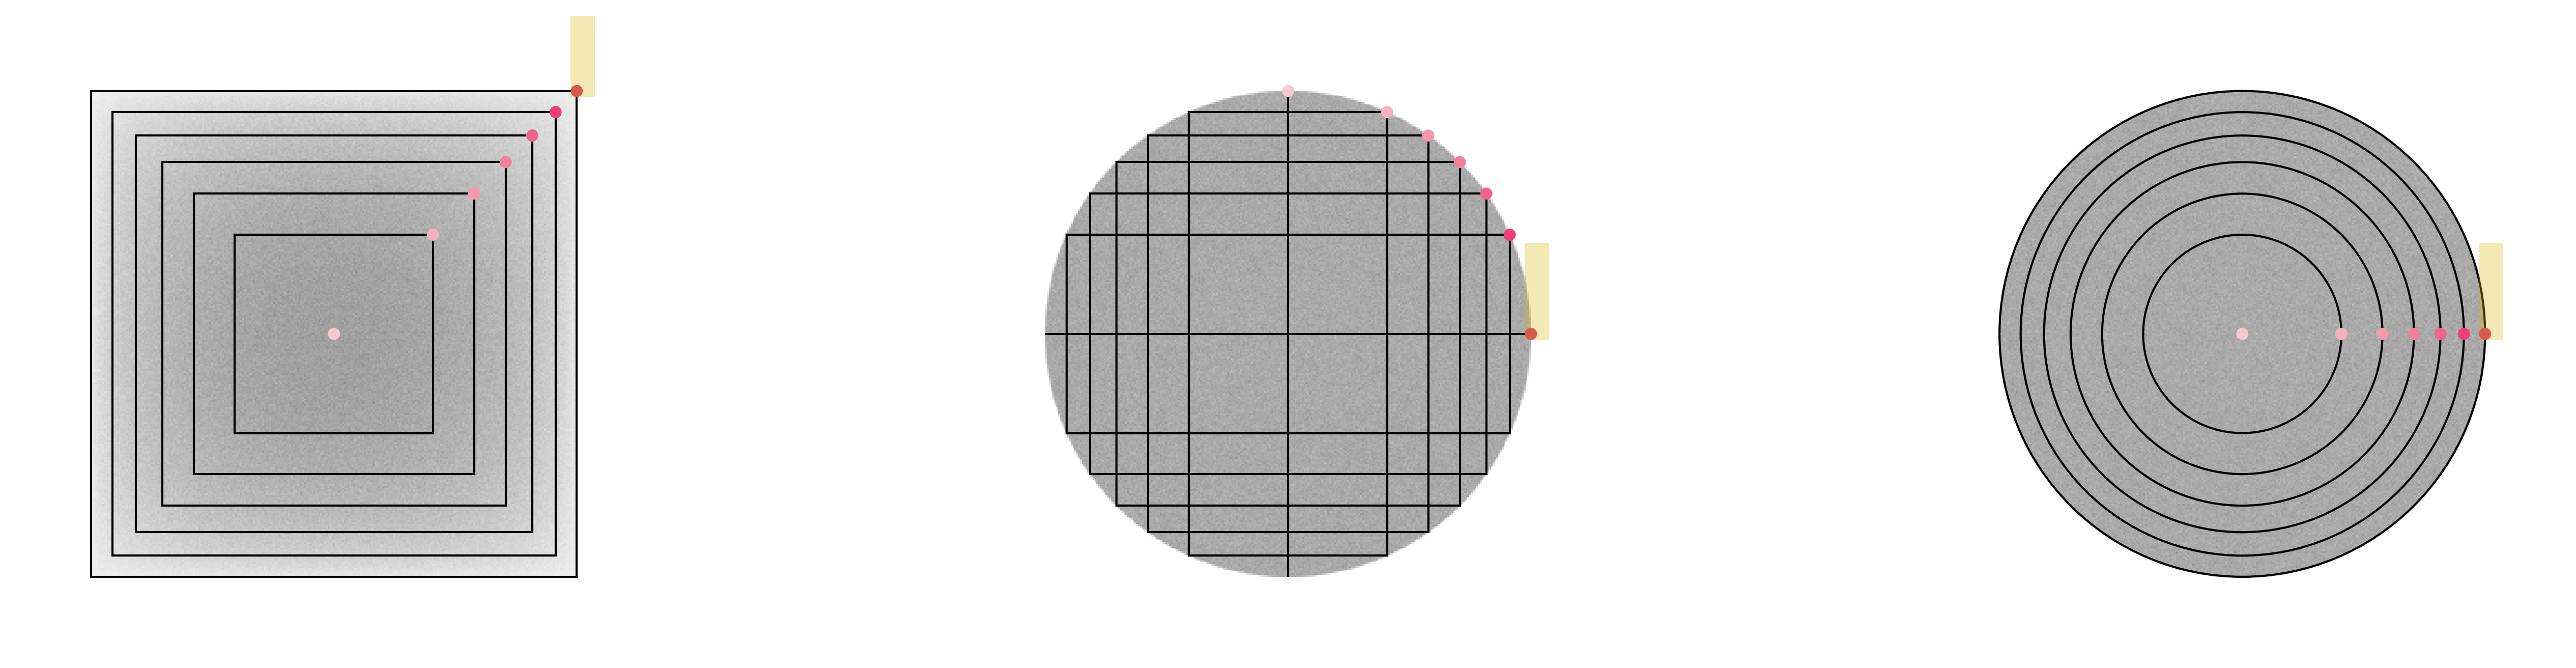
\includegraphics[width=\textwidth]{Images/chapter1/painting_graphic.png}
    \caption{Illustration of correlated painting (left), anti-correlated painting (center), and elliptical painting (right) in the linear approximation without space charge.}
    \label{fig:painting_graphic}
\end{figure}
%
The lightest/darkest pink marker represents the initial/final injection point, and the foil location is indicated by the gold rectangle.\footnote{The foil is not drawn to scale.} Note that this method produces a non-uniform density in the $x$-$y$ plane.

A primary concern in the SNS is the size and peak density of the $x$-$y$ distribution on the spallation target \cite{Riemer2010}. A modified correlated painting scheme is employed to this end:
%
\begin{equation}
\begin{aligned}
    {x}(t) &= x_0 + x_{max}\sqrt{t}, \\
    {y}(t) &= y_0 + y_{max}\sqrt{t}, \\
    x'(t) &= y'(t) = 0.
\end{aligned}
\end{equation}
%
Initially, a donut is created in phase space. Space charge and other nonlinear forces eventually cause the distribution to fill in its hollow center, reducing the peak density.


\subsubsection{Anti-correlated painting}

Anti-correlated painting is equivalent to correlated painting reversed in one of the planes:
%
\begin{equation}
\begin{aligned}
    {x}(t) &= x_{max}\sqrt{t}, \\
    {y}(t) &= y_{max}\sqrt{1 - t}. \\
\end{aligned}
\end{equation}
%
Initially, the $x$-$x'$ distribution is a point while the $y$-$y'$ distribution is a donut. The painting path in this method follows the line $J_x + J_y = constant$, which is the condition of particles in the KV distribution. Thus, in the linear approximation without space charge, the final distribution is a KV distribution. This is illustrated in Fig.~\ref{fig:painting_graphic}. However, the space charge force is nonlinear throughout injection and the KV structure will not be maintained \cite{Crosbie1996}. How to overcome this limitation is an open question. Nonetheless, anti-correlated painting has benefits over correlated painting in some cases \cite{Hotchi2020}.


\subsubsection{Elliptical painting}

Refer back to Eq.~\eqref{eq:eigvec_coords} in which the single-particle motion is written as the sum of two modes. In the elliptical painting method, the injection point $\mathbf{x} = (x, x', y, y')$ is scaled along one of the eigenvectors:
%
\begin{equation}\label{eq:elliptical_painting}
    \mathbf{x}(t) =  
    Re \left\{ \sqrt{2 J_l} \, \mathbf{v}_l \, e^{-i\psi_l} \right\} \sqrt{t},
\end{equation}
%
with $l = 1,2$. The first injected pulse does not move since it is injected onto the closed orbit. The second pulse traces a small ellipse in every 2D projection of the phase space on a turn-by-turn basis. The third pulse traces a slightly larger ellipse enclosing the second, and so on. The square root time-dependence ensures that the beam is a uniform density ellipse in every 2D projection of the 4D phase space at every point during injection. Thus, in the linear approximation, a Danilov distribution is maintained at all times, even with space charge.\footnote{Of course, the method is limited even in the linear approximation due to the finite emittance of the beam from the linac.} This is illustrated on the right side of Fig.~\ref{fig:painting_graphic}.

Elliptical painting can be carried out in any ring. If the ring is uncoupled, the two elliptical modes reduce to planar modes and injection into one of the modes results in a flat beam. Coupled optics change the shape of the matched beam at the injection point and produce a non-flat beam. Alternatively, the horizontal and vertical tunes can be equated, in which case the transfer matrix has degenerate eigenvalues and any linear combination of eigenvectors is itself an eigenvector. This is discussed further in the subsequent chapters.


\subsection{Implementation of elliptical painting in the Spallation Neutron Source}

Elliptical painting requires time-dependent control of the transverse ring orbit position and slope in both planes at the injection point. The SNS is highly-optimized for correlated painting, not elliptical painting, but elliptical painting is possible in principle. A software application to perform the painting method has recently been developed by SNS physicists; before describing the application, a brief description of the SNS is warranted. 

\subsubsection{Description of the Spallation Neutron Source}

The SNS is a neutron scattering facility. Sixty times per second, a microsecond-long proton beam collides with a liquid mercury target at 1 GeV kinetic energy, producing neutrons by the process of spallation \cite{Russell1990}. The original beam is a continuous wave of H$^-$ ions which is chopped and then bunched in a 402.5 MHz radio-frequency quadrupole (RFQ), forming microsecond-long minipulses. Each minipulse is accelerated to 1 GeV through a normal-conducting, then superconducting linac, then transported to the injection region through the high-energy beam transport (HEBT). The electrons are then stripped using a carbon foil, and the remaining protons continue their journey in the ring. One thousand minipulses, or $1.5 \times 10^{14}$ protons, are accumulated over $10^{-3}$ seconds before the beam is extracted and guided through the ring-target beam transport line (RTBT) to the target. A comprehensive description of the SNS is given in \cite{Henderson2014}. Fig.~\ref{fig:SNS} shows an overview of the machine.
%
\begin{figure}[!p]
    \centering
    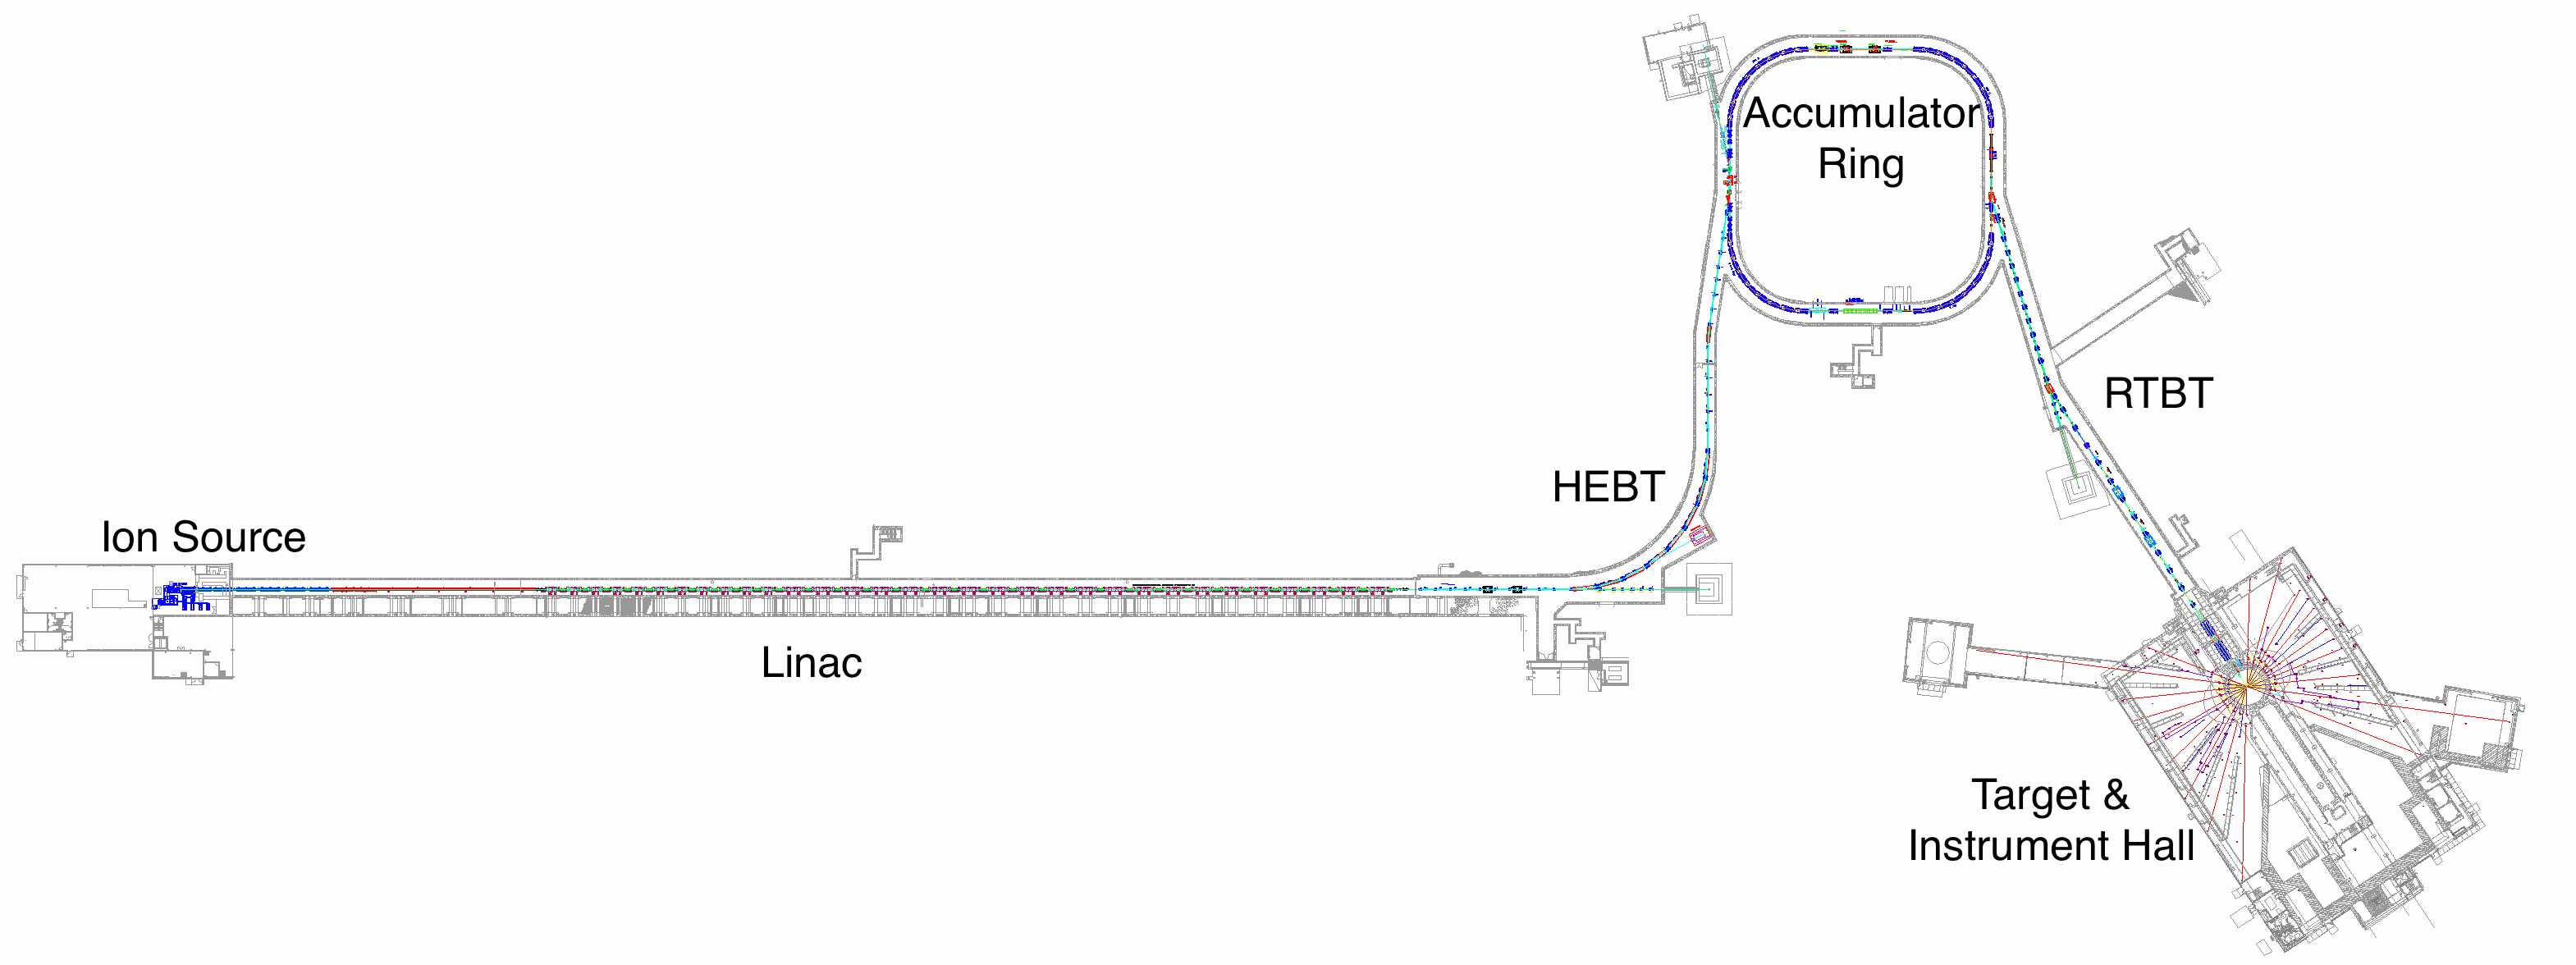
\includegraphics[angle=-90, width=0.5\textwidth]{Images/chapter1/SNS.png}
    \caption{Overview of the Spallation Neutron Source.}
    \label{fig:SNS}
\end{figure}
%

Fig.~\ref{fig:SNS_injection_region} zooms in on the injection region.
%
\begin{figure}[!p]
    \centering
    \begin{subfigure}{\textwidth}
        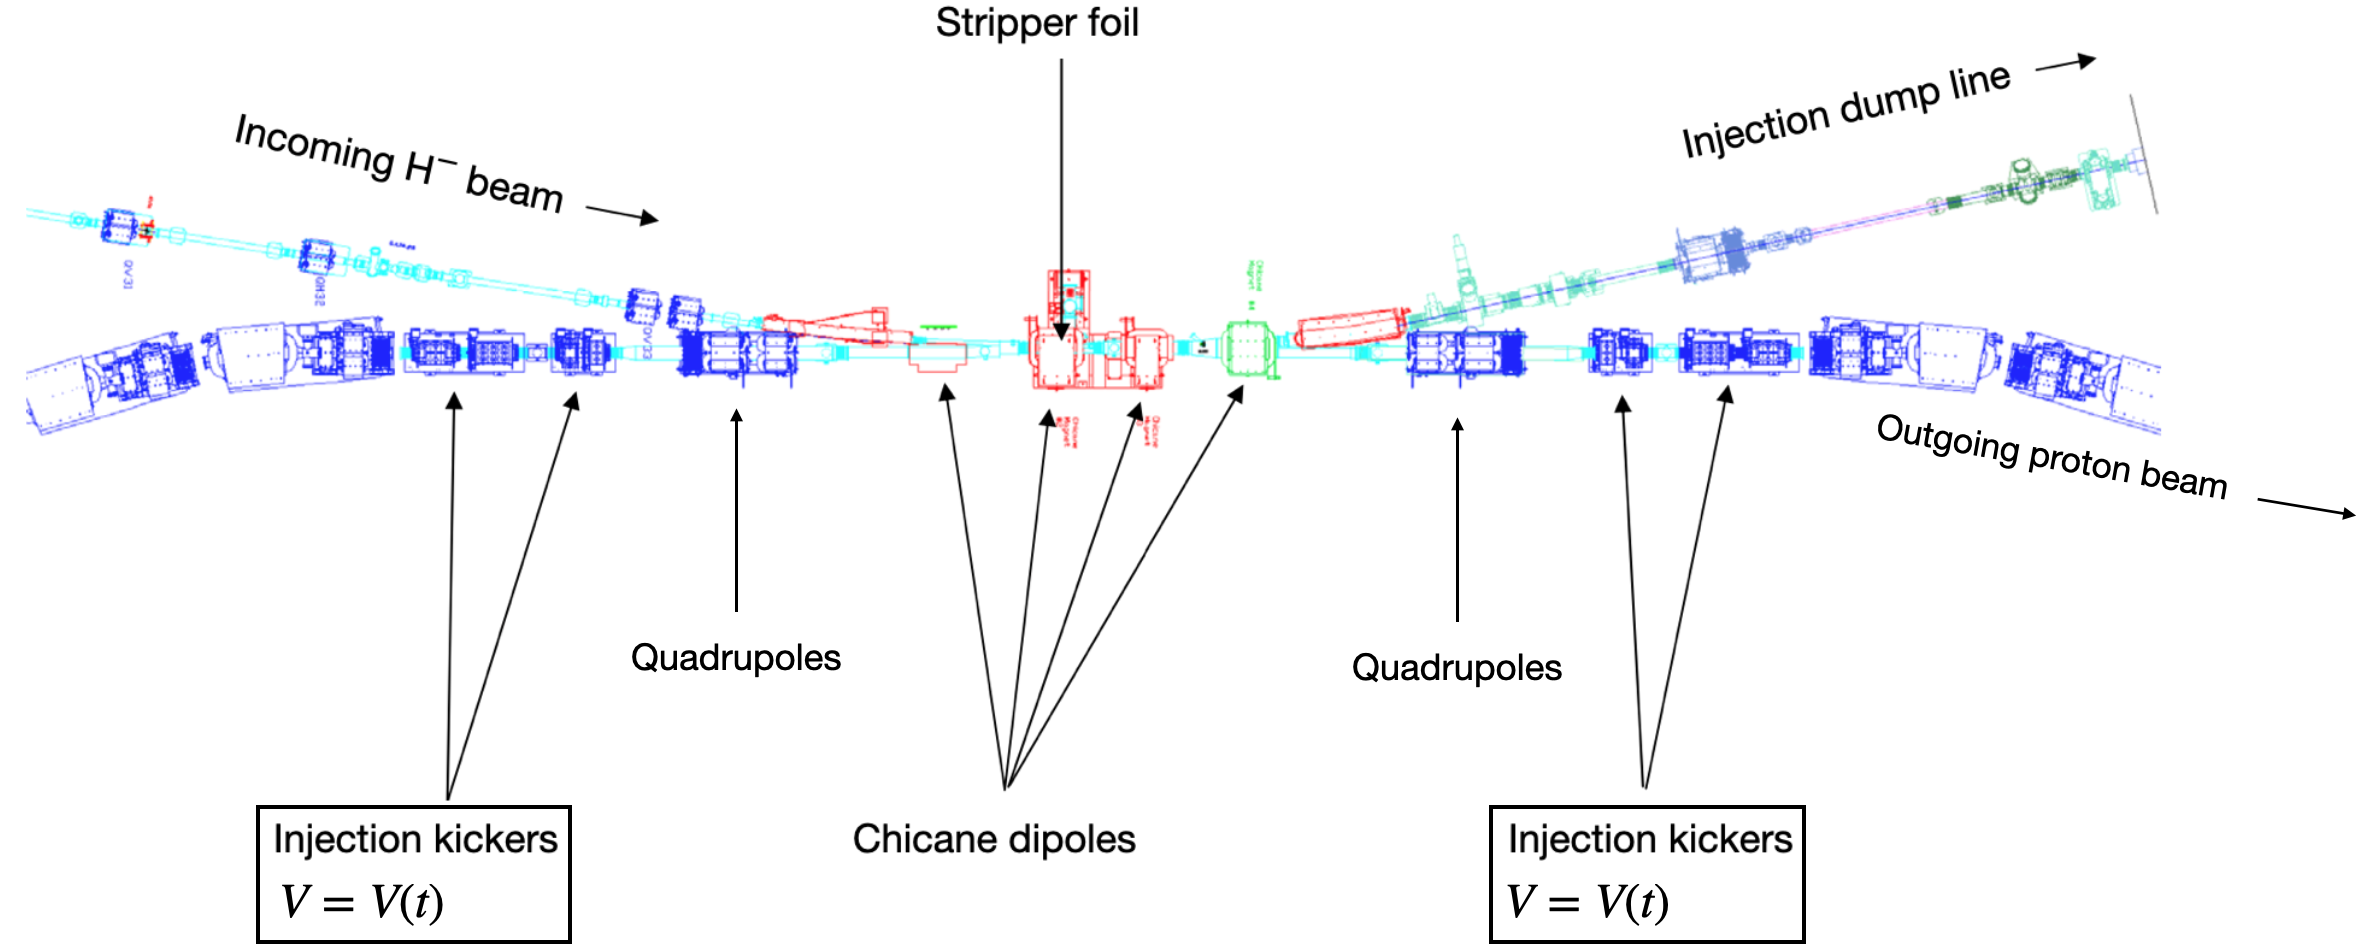
\includegraphics[width=\textwidth]{Images/chapter1/SNS_injection_region1.png}
        \label{fig:SNS_injection_region_a}
        \caption{}
    \end{subfigure}
    \vfill
    \vspace*{1.5cm}
    \vfill
    \begin{subfigure}{\textwidth}
        \centering
        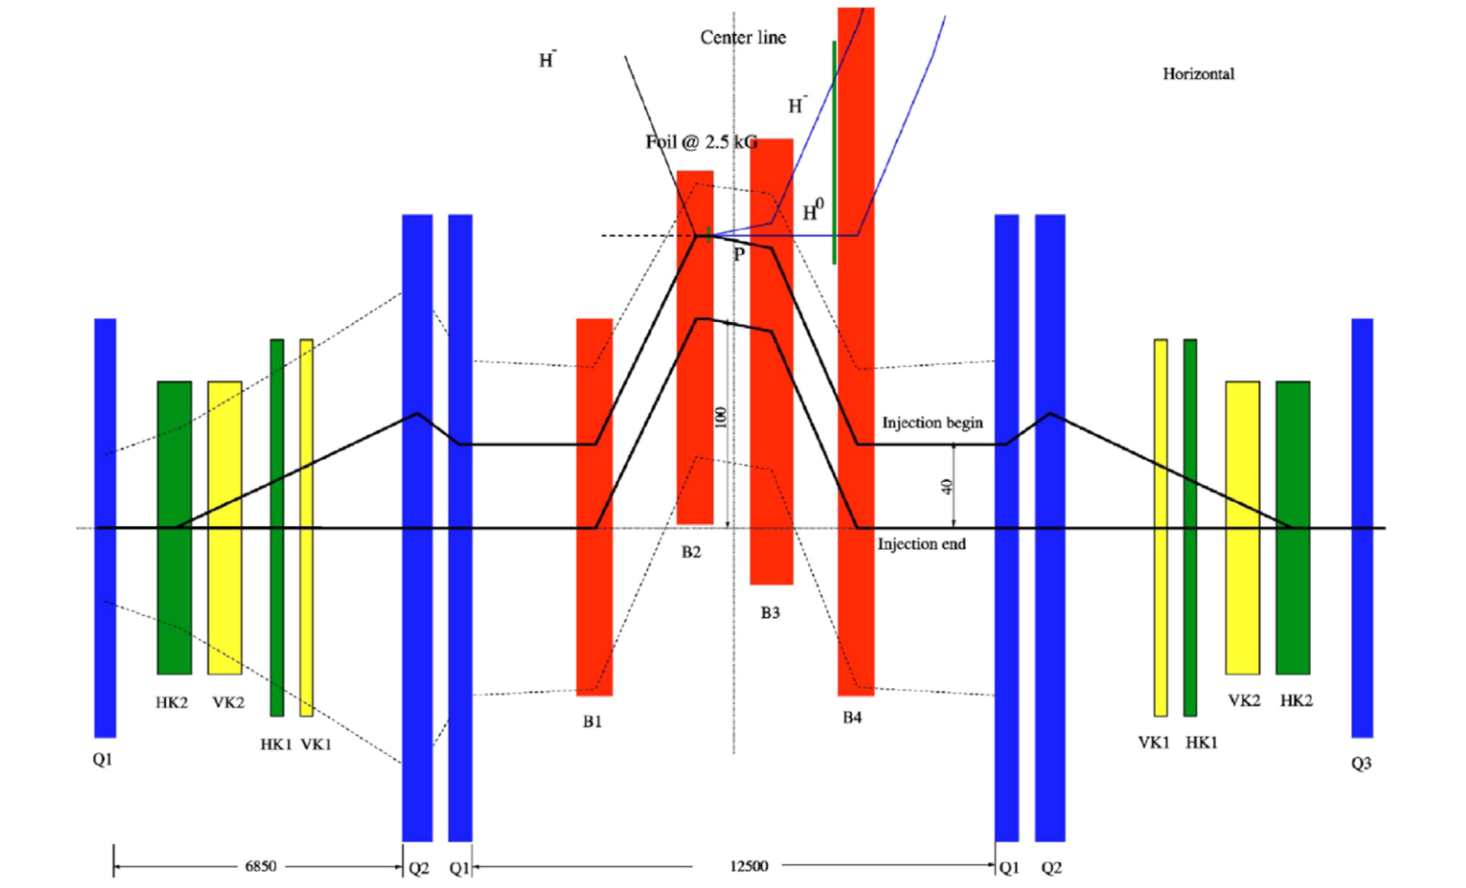
\includegraphics[width=\textwidth]{Images/chapter1/SNS_injection_region_2b.png}
        \caption{}
        \label{fig:SNS_injection_region_b}
    \end{subfigure}
    \caption{SNS injection region. (a) Overhead view of H$^-$ beam trajectory. (b) Schematic layout of the horizontal plane of the injection region: red = chicane dipoles, blue = quadrupoles, green = horizontal kickers, yellow = vertical kickers. (From \cite{Henderson2014}.)}
    \label{fig:SNS_injection_region}
\end{figure}
%
Four dipole magnets align the horizontal orbit with the beam from the linac at the foil. The injected beam trajectory is held fixed so that any remaining H$^0$ or H$^-$ particles can be reliably guided to a dump. Eight kicker magnets — four per plane — are available for time-dependent control of the position and slope of the orbit at the injection point. 


\subsubsection{Ring Injection Control application}

Each injection kicker magnet is given a waveform that scales the kicker voltage during injection. Once the initial and final voltages are known, they can be connected with a square root waveform to satisfy Eq.~\eqref{eq:elliptical_painting}. The final beam intensity is controlled by the painting time — time between the initial and final voltages.

To control the position and angle of the orbit at the injection point, it is first necessary to measure the position and angle of the orbit at the injection point. This can be done indirectly as follows. A single minipulse is injected and stored in the ring, and its turn-by-turn mean transverse position is measured using a beam-position-monitor (BPM). This is repeated for several minipulses and the average is taken. In the linear approximation, the mean position performs the pseudo-harmonic oscillations of Eq.~\eqref{eq:Hill_solution}; however, energy spread in the minipulse eventually sends the mean position to zero. For a Gaussian energy spread, a damped sine wave is an accurate model of this process \cite{Pelaia2016}:
%
\begin{equation}\label{eq:damped_sinusoid}
    x(t) = A_0 + A e^{kt^2} \cos{\left(\mu + \mu_0\right)},
\end{equation}
%
where $t$ is the turn number. The parameter $A$ gives the betatron amplitude, $\mu / 2\pi$ gives the fractional tune, and $\mu_0$ gives the particle phase at the BPM. The phase space coordinates are recovered by combining these parameters with the linear ring model:
%
\begin{equation}
\begin{aligned}
    x_{bpm} &= A \cos\mu_0 \\ 
    x'_{bpm} &= -A\left({\sin\mu_0 + \frac{\alpha}{\beta}\cos\mu_0}\right).
\end{aligned}
\end{equation}
%
The coordinates are then transported to the injection point using the model transfer matrix. Repeating this for each BPM gives an estimated mean and standard deviation of the phase space coordinates at the injection point. Examples of measured individual and averaged BPM signals in the SNS ring are shown in Fig.~\ref{fig:bpm_avg} along with the damped-sinusoid fit. Additionally, a simulated minipulse in the (linearized) SNS ring is shown in Fig.~\ref{fig:minipulse}.
%
\begin{figure}[!p]
    \centering
    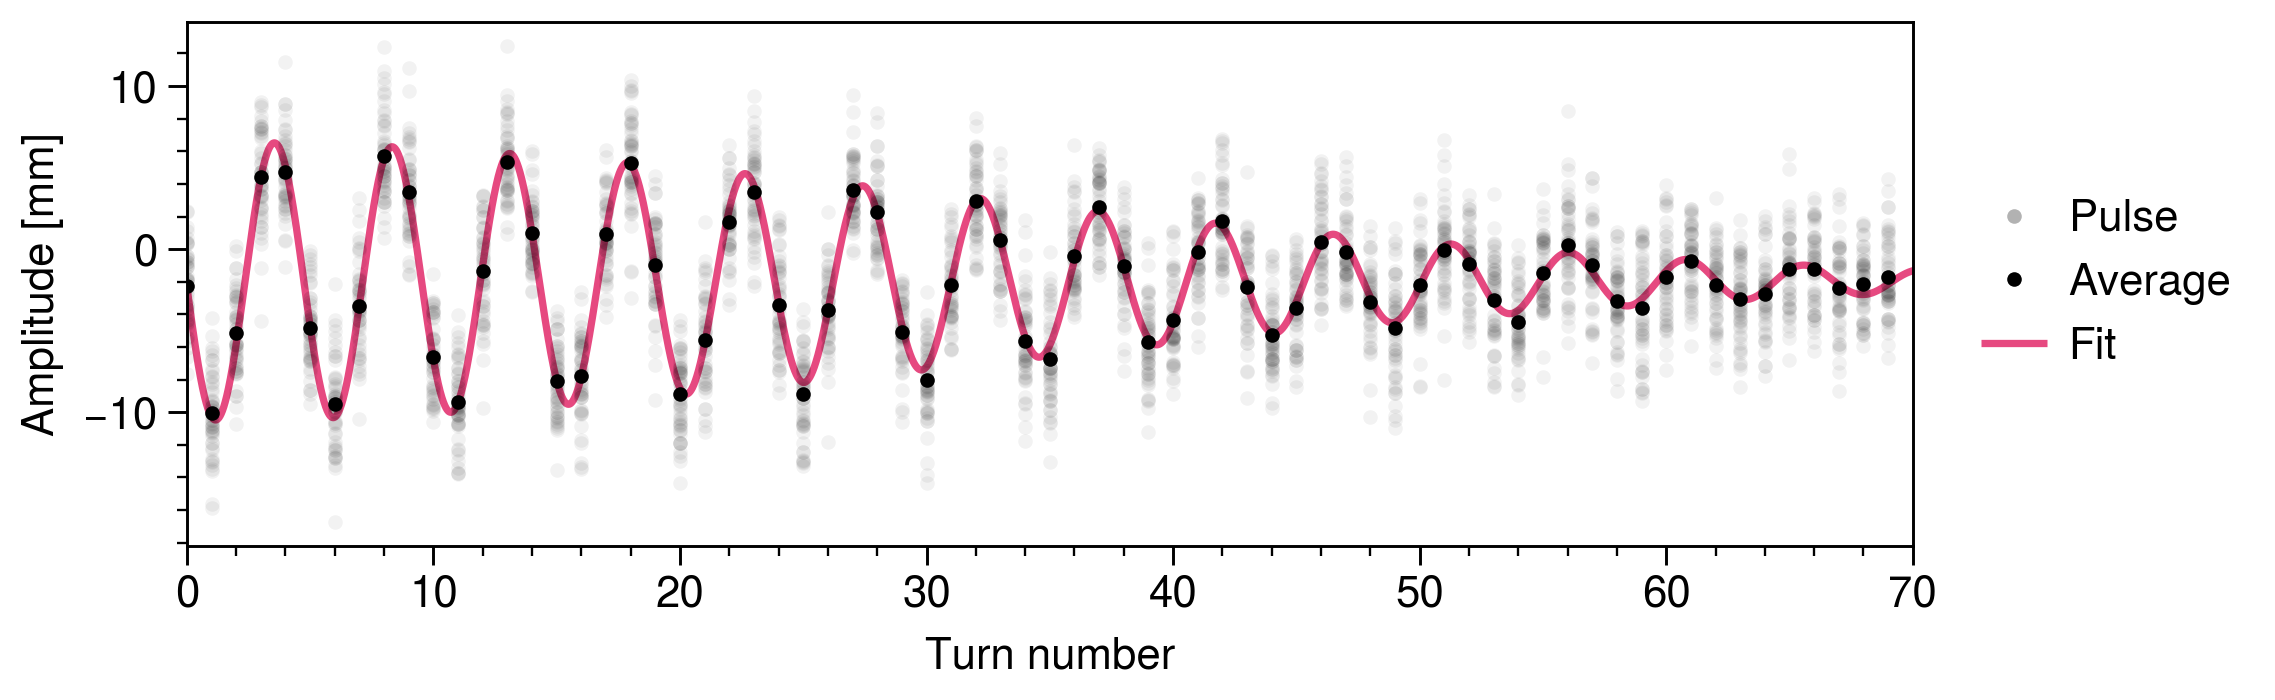
\includegraphics[width=\textwidth]{Images/chapter1/bpm_avg.png}
    \caption{Measured turn-by-turn BPM signal in the SNS ring — averaged over 50 pulses and fit with Eq.~\eqref{eq:damped_sinusoid}.}
    \label{fig:bpm_avg}
\end{figure}
%
%
\begin{figure}
    \centering
    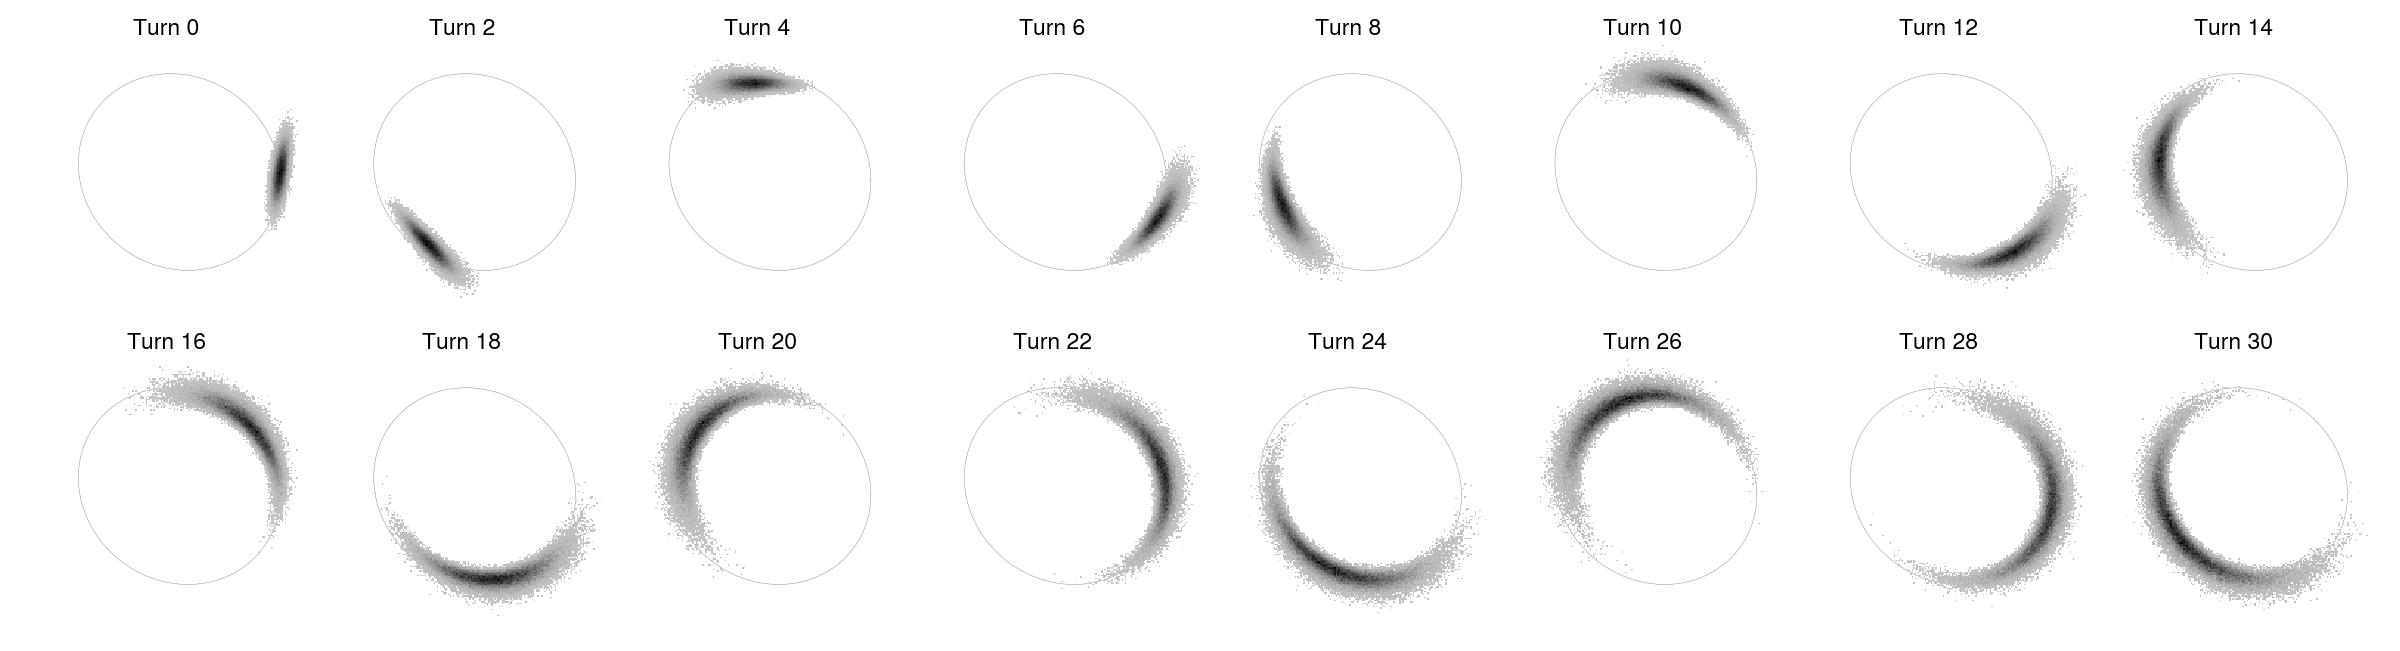
\includegraphics[width=\textwidth]{Images/chapter1/minipulse_chromaticity_black.png}
    \caption{Simulated minipulse in the (linearized) SNS ring. The $x$-$x'$ distribution is plotted at the injection point along with the Courant-Snyder ellipse.}
    \label{fig:minipulse}
\end{figure}
%

The next issue is how to control phase space coordinates at the injection point. Each kicker magnet is calibrated by applying a voltage difference to the magnet and measuring the orbit response using the ring BPMs; the angular kick associated with the magnet is varied until the model orbit agrees with the measured orbit. It was found that slight quadrupole corrections are necessary for this to occur. The standard deviation of the measured phase space coordinates is small after this calibration. One can then ask the model for a change in coordinates, update the kickers accordingly, and measure the new coordinates, iterating if necessary. This is currently done manually, and kicker power supplies need to be visually checked to make sure they are not beyond physical limits. Once this setup is complete, the kicker voltages are saved to a file and fed to a different script which scales sets the kicker waveforms. These steps were implemented as part of the Ring Injection Control (RIC) application in the OpenXAL framework \cite{Milas2021}. 

SNS injection kicker magnets have limited strengths and are unipolar, which limits the maximum relative angle between the HEBT trajectory and the ring orbit at the injection point. As discussed later, there are several tricks that can be played to increase the effective injection kicker strength, one of which is to decrease the beam energy; however, this is a significant task due to issues related to the SNS timing system. Initial attempts to lower the energy to 0.6 GeV were successful, but difficult and time-consuming. An energy of 0.8 GeV appears to be the minimum energy achievable within the time-frame of a single beam physics experiment.


\section{Structure and goals of this dissertation}\label{sec:Goals of this dissertation}.

The primary goal of this dissertation is to contribute to efforts to produce a Danilov distribution in the SNS ring. A secondary goal is to improve the current understanding of the dynamics of the Danilov distribution with space charge.

In Chapter \ref{chap-2}, the envelope equations describing the linear transport of the Danilov distribution are used to calculate the matched beam envelope with the inclusion of space charge forces. Such a calculation is critical to producing a Danilov distribution in a ring using the elliptical painting method. In Chapter \ref{chap-3}, the computational model used for realistic simulations of beam dynamics in the SNS ring is described. Previously published simulation results will be re-examined. The significance of updated experimental constraints will be discussed. In Chapter \ref{chap-4}, several methods will be proposed to measure the similarity between a painted distribution in the SNS ring and a Danilov distribution. The implementation of these methods in the SNS will be discussed. In Chapter \ref{chap-5}, the results of initial experimental studies of elliptical painting in the SNS will be presented. Simulations will be provided to aid in interpreting the results. In Chapter \ref{chap-6}, implications and extensions of this work will be discussed.
\chapter{Beam envelope equations} \label{chap-2}

In this chapter, the dynamics of the Danilov distribution are investigated using the envelope model. First, the envelope equations for the Danilov distribution are presented. Second, a method to find the matched beam envelope with space charge is developed. The method is demonstrated in several simple focusing systems and the properties of the solutions are examined. Third, the matched beam envelope in a linearized version of the SNS ring is calculated and the practical importance of the calculation is discussed.\footnote{The majority of this chapter has been published in \cite{Hoover2021}.}


\section{The Danilov envelope equations}

We seek a self-consistent set of differential equations for the elliptical boundary containing the beam particles, similar to Eq.~\eqref{eq:KV_envelope}. Although Chernin's equations satisfy this requirement \cite{Chernin1988}, we adopt the equations derived in \cite{Danilov2003}. There, the coordinates of the ellipse in real space are parameterized as $\mathbf{x} = \mathbf{W}\mathbf{c}$ where $\mathbf{x} = (x, y)^T$, $\mathbf{W}$ is the $2 \times 2$ envelope matrix, $\mathbf{c} = (\cos\psi, \, \sin\psi)^T$, and $\psi$ is a free parameter running from $0$ to $2\pi$. The envelope matrix evolves according to
%
\begin{equation}\label{eq:danilov_envelope}
    \mathbf{W}'' + \left({\mathbf{K_0} - \mathbf{K}_{sc}}\right)\mathbf{W} + \mathbf{K}_1 \mathbf{W}'= 0,
\end{equation}
%
where $\mathbf{K}_0$, $\mathbf{K}_1$, and $\mathbf{K}_{sc}$ are time-dependent $2 \times 2$ matrices. Linear external focusing is encompassed by $\mathbf{K}_{0, 1}$, and linear space charge defocusing is encompassed by $\mathbf{K}_{sc}$. If the beam ellipse in real space has semi-axes $c_x$ and $c_y$ and is tilted at an angle $\phi$ below the $x$ axis, then
%
\begin{equation}
    \mathbf{K}_{sc} = \frac{2Q}{c_x + c_y} 
        \mathbf{R}(\phi) \begin{bmatrix} 1/c_x & 0 \\ 0 & 1/c_y \end{bmatrix} \mathbf{R}(\phi)^T. 
\end{equation}
%
$\mathbf{R}$ is the rotation matrix and $Q$ is the beam perveance (Eq.~\eqref{eq:perveance}). When Eq.~\eqref{eq:danilov_envelope} is expanded, the evolution of each envelope matrix element resembles that of a single particle in a linear system with a nonlinear driving term proportional to $Q$. Thus, the equations can be easily integrated using an existing tracking code such as PyORBIT \cite{Shishlo2015}. The four elements of $\mathbf{W}$ are represented using two bunch particles, and nodes are added to the accelerator model to perform the nonlinear kicks. 

The integration of Eq.~\eqref{eq:danilov_envelope} reveals that the Danilov distribution tilts in real space even without coupled forces; this is illustrated in Fig.~\ref{fig:fodo_zerosc}. 
%
\begin{figure}[!p]
    \centering
    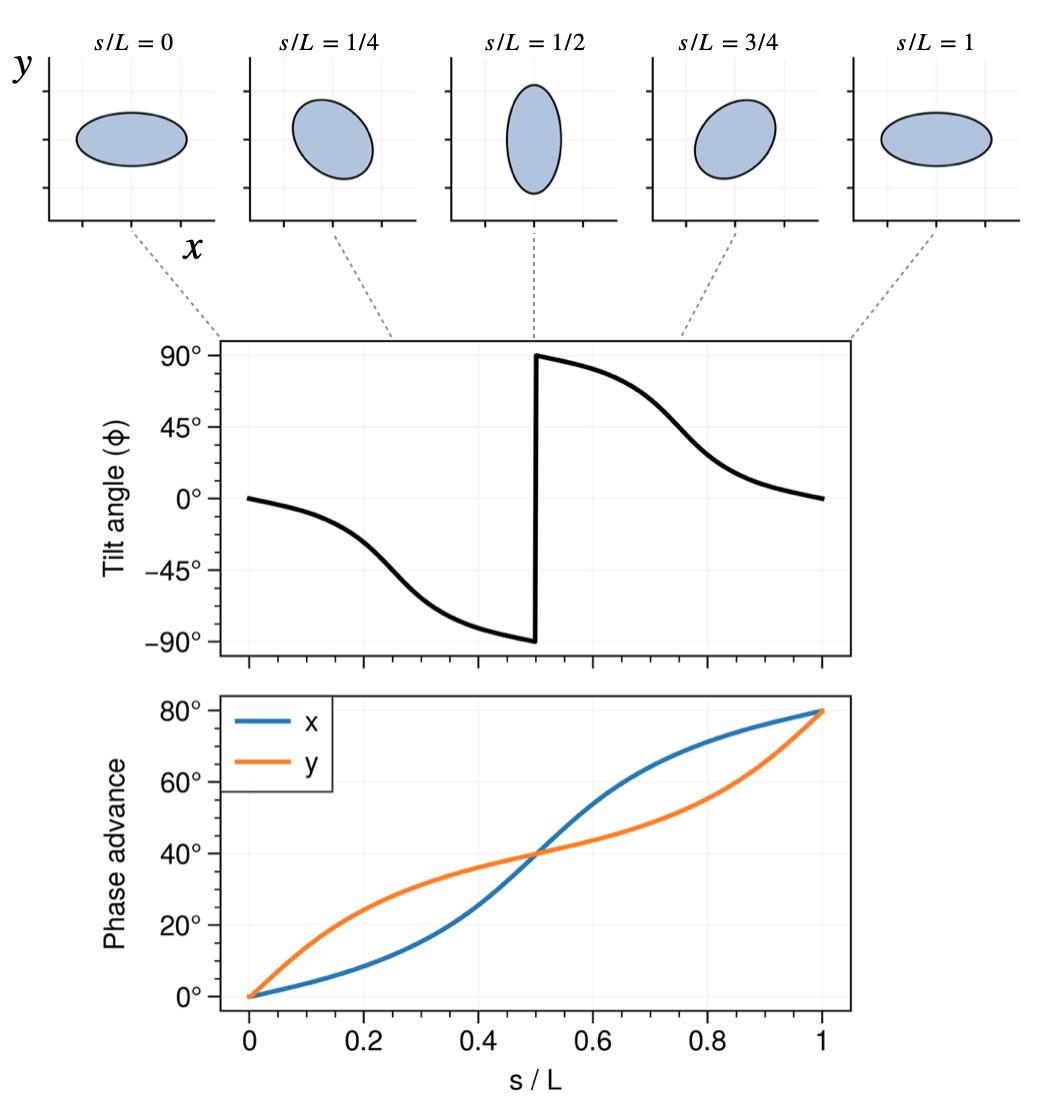
\includegraphics[width=0.8\textwidth]{Images/chapter2/fodo_zerosc.png}
    \caption{Relationship between the tilt angle in real space and the $x$ and $y$ phase advances for a Danilov distribution in a FODO cell of length $L$. The beam is tracked without space charge by integrating the envelope equations.}
    \label{fig:fodo_zerosc}
\end{figure}
%
The tilt angle is a function of the difference between the horizontal and vertical phase advances, which are calculated from
\begin{equation} \label{eq:phase_advance}
    \mu_x(s) = \int_{0}^{s}
    {\frac{\varepsilon_x(s')}{{\tilde{x}(s')}^2} \, ds'},
\end{equation}
where $\tilde{x}^2 = \langle{x^2}\rangle$ and $x$ and $y$ can be interchanged.



\section{Matched envelope computation}

The distribution function $f$ of a matched beam in a lattice of period length $L$ satisfies $f(s) = f(s + L)$ for all $s$. In practice, matching usually refers only to the second-order moments contained in the beam covariance matrix: $\bm{\Sigma}(s) = \bm{\Sigma}(s + L)$. The two notions are equivalent for the Danilov distribution, for which all higher-order moments vanish.

The problem of computing the matched beam is as follows:
%
\begin{equation}
\begin{aligned}
    & \underset{\bm{\Sigma}}{\text{minimize}}
    & & C(\bm{\Sigma}) = \left\Vert{\mathbf{M} \bm{\Sigma} \mathbf{M}^T - \bm{\Sigma}}\right\Vert^2 \\
    & \text{subject to}
    & & |\bm{\Sigma}| = 0,
\end{aligned}
\end{equation}
%
where $\mathbf{M} = \mathbf{M}(\bm{\Sigma})$ is a linear transfer matrix connecting the initial and final covariance matrix, and $\Vert\dots\Vert$ is the matrix norm. The constraint that the covariance matrix is singular comes from the definition of the Danilov distribution. Additionally, we would like to hold the nonzero intrinsic emittance fixed so that a unique solution is found for a given lattice and beam perveance. An iterative approach is needed since space charge causes $\mathbf{M}$ to depend on $\bm{\Sigma}$ in a potentially complicated way which is unknown before tracking the beam. 


\subsection{Motivation}

The calculation of the matched beam envelope is of practical importance for space-charge-dominated beams. It is a common first step in lattice design \cite{Lund2006}. The beam current able to be transported through a periodic focusing channel with a given aperture is maximum when the beam is matched \cite{book:Reiser}. The free energy available in a mismatched beam may result in emittance growth and halo formation \cite{book:Reiser}. Calculation of the matched envelope is generally the first step in a stability analysis of the KV envelope equations \cite{Lund2006}. The task has been performed for the KV distribution in both uncoupled and coupled focusing systems \cite{Hofmann1983, Chernin1988, Ryne1995, Lund2006, Anderson2007, Goswami2016}, and it would be beneficial to extend this analysis to the Danilov distribution. Furthermore, the calculation of the matched envelope of the Danilov distribution is of critical importance to the experimental realization of such a distribution: the result of the elliptical painting method only approaches a Danilov distribution if the circulating beam is matched.

The purpose of this section is to calculate and describe the properties of the matched envelope of the Danilov distribution in simple focusing systems as space charge is increased. In addition to the ability to calculate the matched envelope in more complicated focusing systems such as the SNS accumulator ring, a better understanding of the beam dynamics under the influence of coupled internal and external forces should fall out of this analysis.

Before presenting our solution, we highlight the space-charge-driven mismatch oscillations that are to be corrected. Fig.~\ref{fig:fodo_mismatch_tbt} shows the turn-by-turn evolution of a beam that is matched to a lattice without space charge and then tracked with space charge. 
%
\begin{figure}[!p]
    \centering
    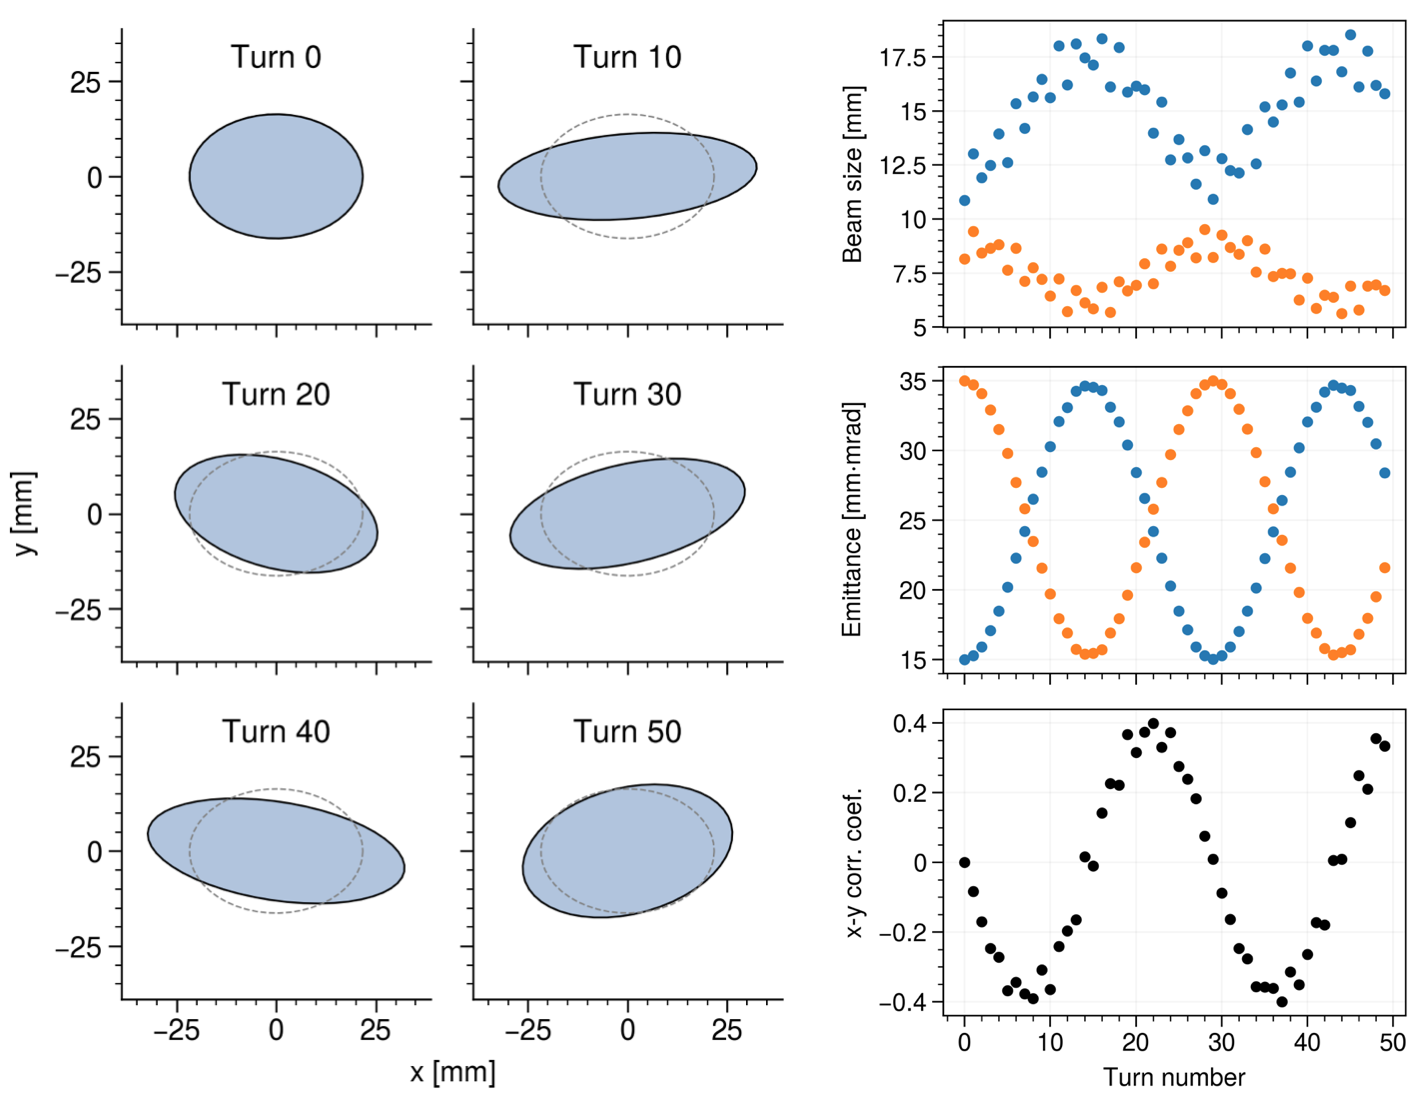
\includegraphics[width=\textwidth]{Images/chapter2/fodo_mismatch_tbt.png}
    \caption{Turn-by-turn mismatch oscillations of the Danilov distribution at the entrance of an uncoupled FODO lattice. The beam would be matched to the lattice without space charge. In the right column, blue (orange) corresponds to $x$ ($y$).}
    \label{fig:fodo_mismatch_tbt}
\end{figure}
%
There are two frequencies in the mismatch oscillations: a larger frequency near twice the zero-current tune corresponding to the breathing oscillation of the beam sizes, and a smaller frequency corresponding to the emittance exchange from space-charge-driven linear coupling. 


\subsection{Solution}

The problem of computing the matched envelope can be approached in the following way. The effect of the linear beam space charge is to modify the linear focusing strength at every position; we call this modified linear focusing system the \textit{effective lattice}. Generating a beam that is matched to a lattice with space charge is equivalent to generating a beam that is matched to an effective lattice without space charge. The latter task is straightforward using an existing parameterization of coupled motion. The correct effective lattice is unknown a priori, so a search must be performed over the parameters. Fig.~\ref{fig:effective_lattice} illustrates the concept of the effective lattice.
%
\begin{figure}
    \centering
    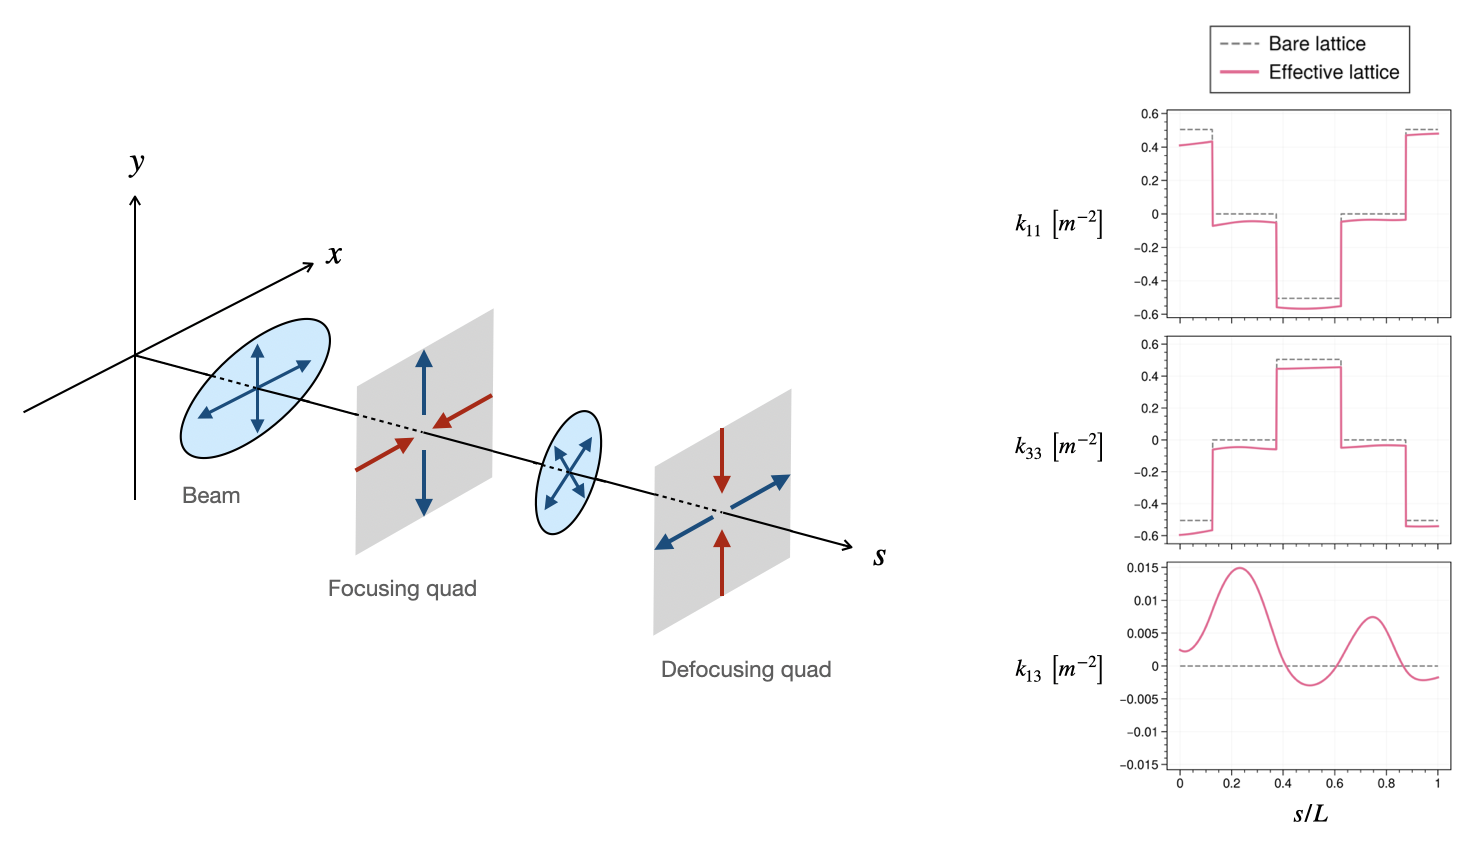
\includegraphics[width=1.0\textwidth]{Images/chapter2/effective_lattice.png}
    \caption{Illustration of the effective lattice — the net linear focusing after space charge is included. The coefficients $k_{ij}$ are defined by $x'' + k_{11}x + k_{13}y = 0$; $y'' + k_{33}y + k_{31}x = 0$.}
    \label{fig:effective_lattice}
\end{figure}
%

\subsubsection{Zero space charge}

We begin by demonstrating how to compute the matched envelope without space charge. We write Eq.~\eqref{eq:eigvec_coords} again for convenience:
%
\begin{equation}
    \mathbf{Mx} = Re \left\{
        \sqrt{2 J_1} \, \mathbf{v}_1 \, e^{-i(\psi_1 + \mu_1)}
        + \sqrt{2 J_2} \, \mathbf{v}_2 \, e^{-i(\psi_2 + \mu_2)}
    \right\}.
\end{equation}
%
The turn-by-turn trajectory of a particle with a given $J_{1,2}$ forms a closed surface in phase space, and a group of particles distributed uniformly over this surface will appear to be invariant. A matched distribution is a collection of these surfaces with different amplitudes.

We now switch to the collective description of the beam using its covariance matrix. The symplectic normalization matrix $\mathbf{V}$ (from Eq.~\eqref{eq:V_from_eigvecs}) can be used to express the matched beam covariance matrix as
%
\begin{equation}\label{eq:sigma_n}
    \bm{\Sigma} = 
    \mathbf{V}
    \begin{bmatrix}
        \varepsilon_1 & 0 & 0 & 0 \\
        0& \varepsilon_1 & 0 & 0 \\
        0 & 0 & \varepsilon_2 & 0 \\
        0 & 0 & 0 & \varepsilon_2
    \end{bmatrix}
    \mathbf{V}^T.
\end{equation}
%
In the uncoupled case, $\mathbf{V}^{-1}$ transforms a tilted ellipse in the $x$-$x'$ plane into a circle. In the coupled case, $\mathbf{V}^{-1}$ transforms a ``tilted" 4D ellipsoid into an ``upright" 4D ellipsoid. A parameterization of $\mathbf{V}$ was introduced in Fig.~\ref{fig:twiss4D}. The number of parameters can be reduced to six by observing that the Danilov distribution is a function of only one eigenvector. We now set one of the intrinsic emittances to zero in Eq.~\eqref{eq:sigma_n} and display the connection between the parameters and the covariance matrix. The beta functions give the ratios between the beam size and intrinsic emittance:
%
\begin{equation}
    \beta_{lx} = \frac{\langle{x^2}\rangle}{\varepsilon_l}, \quad
    \beta_{ly} = \frac{\langle{y^2}\rangle}{\varepsilon_l}
\end{equation}
%
where $l = 1$ or $2$. Similarly, the alpha functions give the ratios between the beam divergence and the intrinsic emittance:
%
\begin{equation}
    \alpha_{lx} = -\frac{\langle{xx'}\rangle}{\varepsilon_l}, \quad
    \alpha_{ly} = -\frac{\langle{yy'}\rangle}{\varepsilon_l}
\end{equation}
%
Next, $u$ gives the ratio between the apparent emittance and the intrinsic emittance. When $l = 1$, $u = \varepsilon_y / \varepsilon_l$, or when $l = 2$, $u = \varepsilon_x / \varepsilon_2$. Finally, $\nu_l$, is related to the $x$-$y$ correlation coefficient:
%
\begin{equation}
    \cos\nu_l = \frac{\langle{xy}\rangle}{\sqrt{\langle{x^2}\rangle\langle{y^2}\rangle}}.
\end{equation}
%
The subscript will be dropped from now on since it has no effect. As mentioned in Fig.~\ref{fig:fodo_zerosc}, $\nu$ will vary even without the presence of coupled forces. For example, Fig.~\ref{fig:splittunes_tbt} shows the turn-by-turn $x$-$y$ projection of a beam whose $x$-$x'$ and $y$-$y'$ ellipses are matched to an uncoupled lattice with a tune separation of 0.01, along with the value of $\nu$ at each frame. 
%
\begin{figure}[!p]
    \centering
    \vspace*{2cm}
    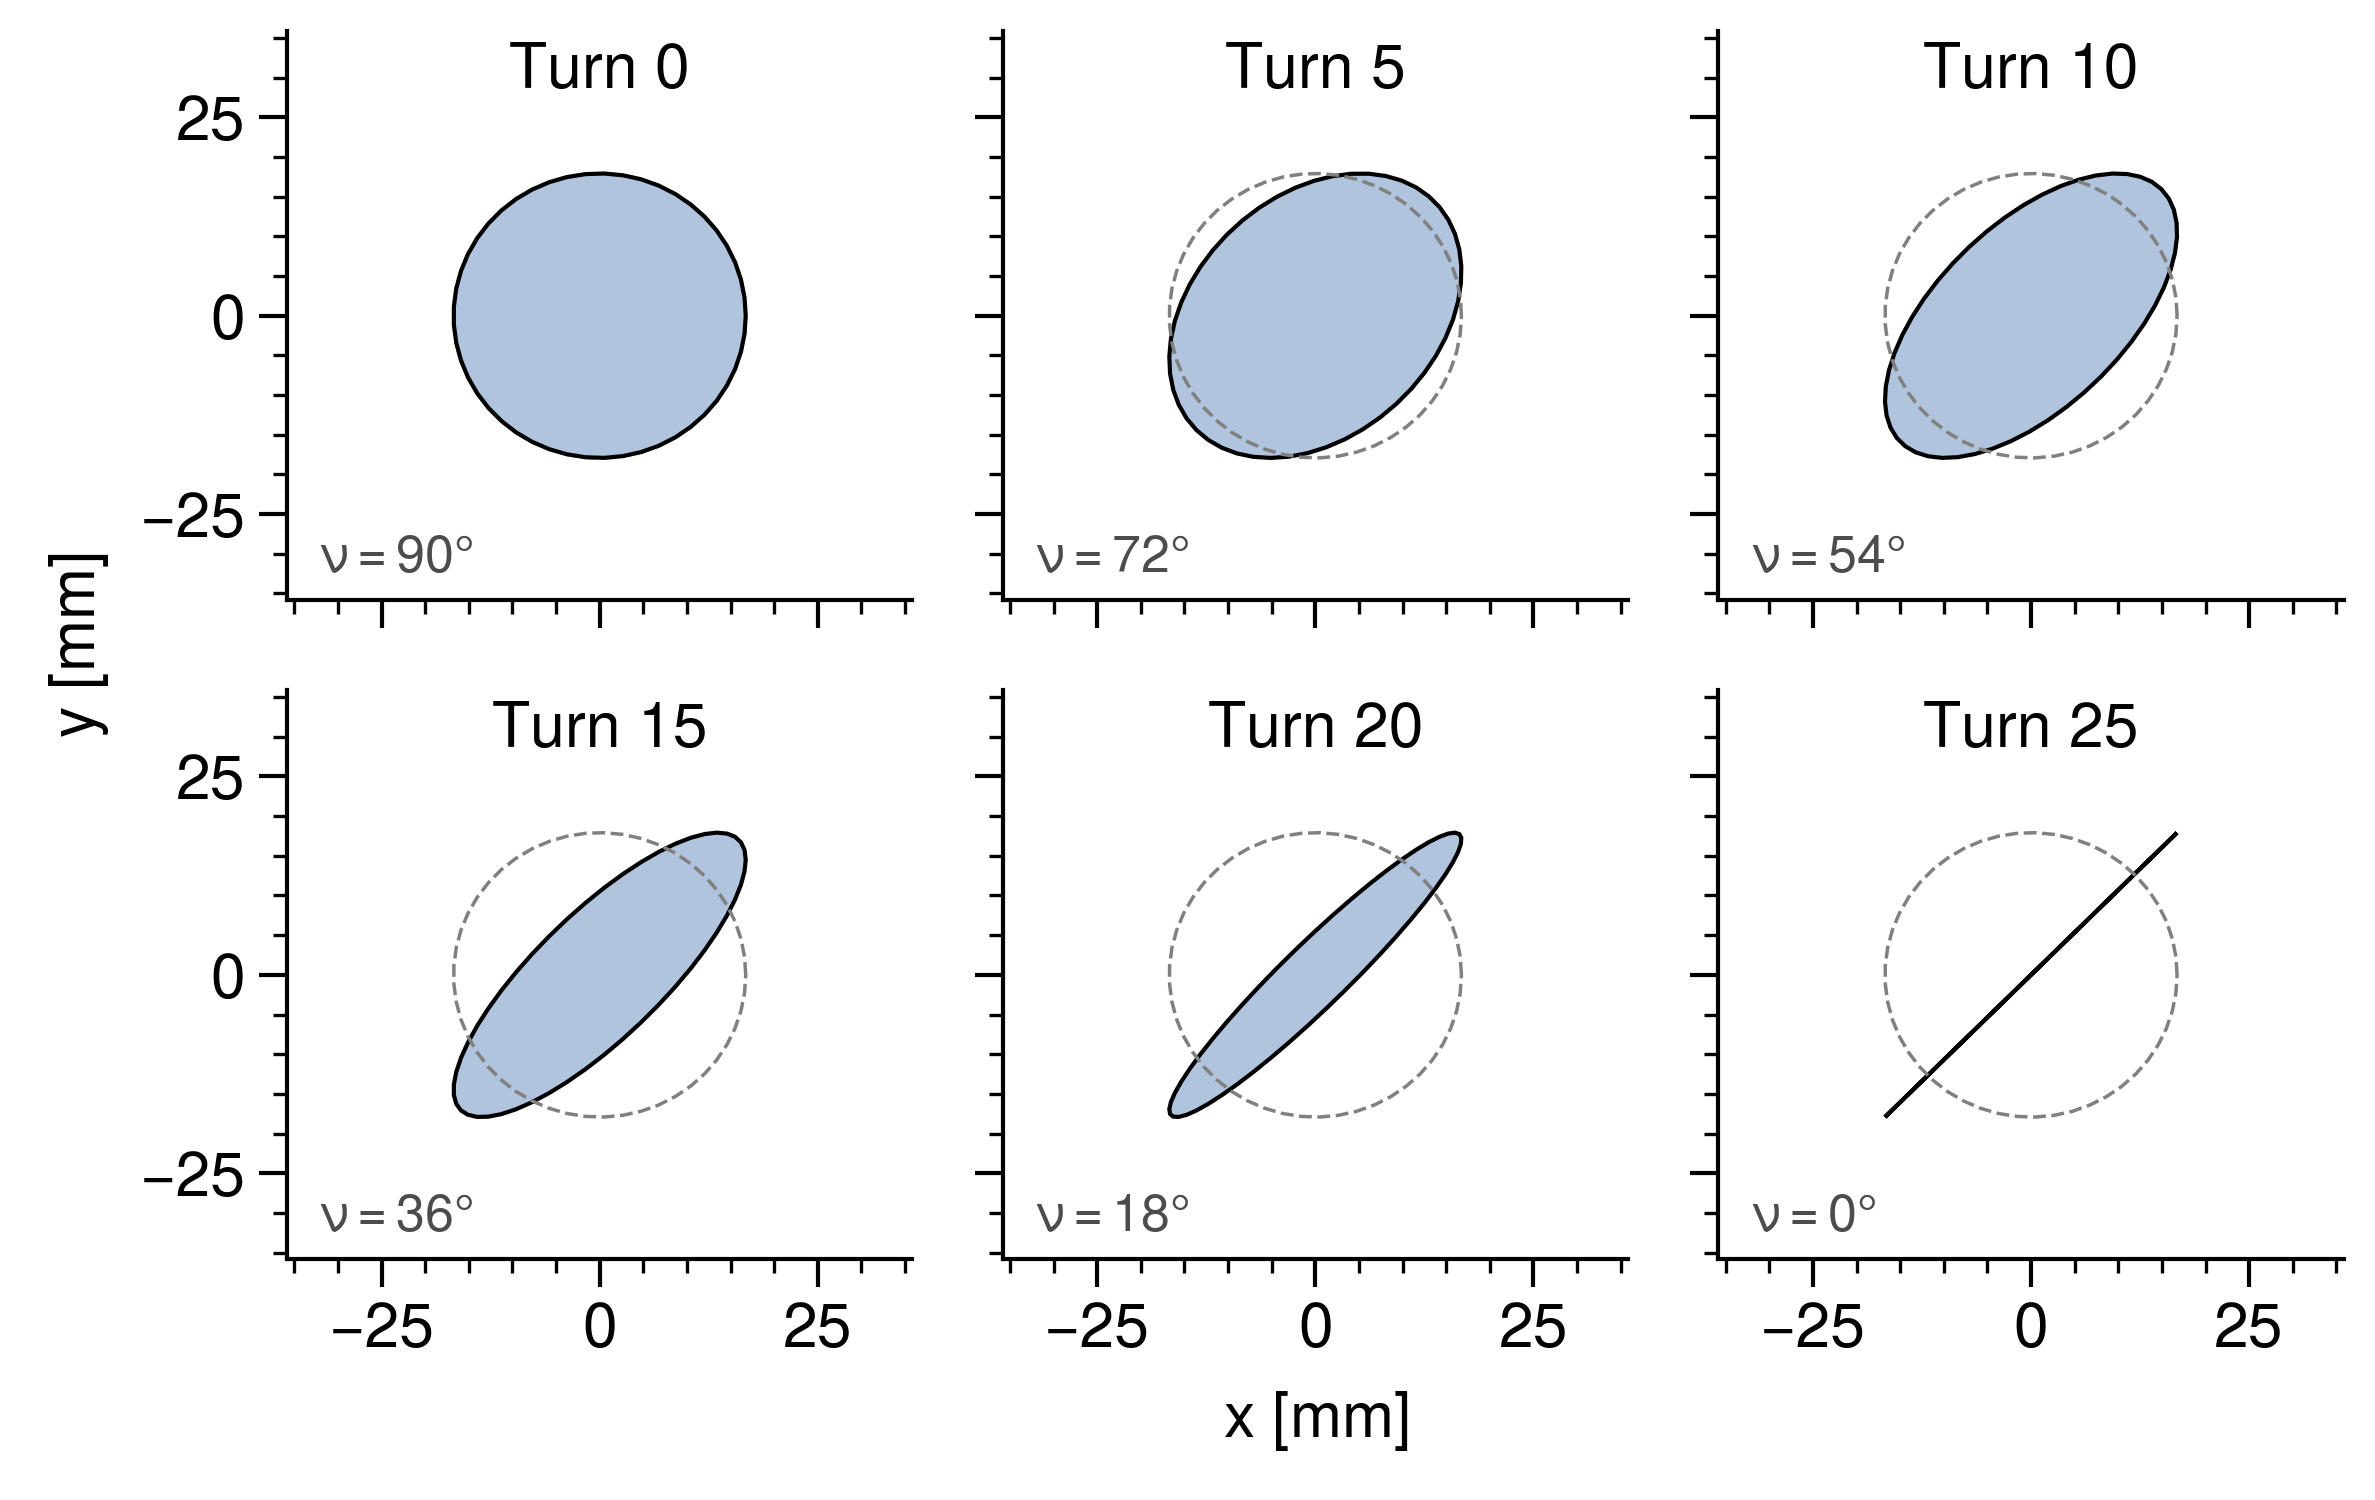
\includegraphics[width=0.8\textwidth]{Images/chapter2/splittunes_tbt.png}
    \caption{Turn-by-turn $x$-$y$ projections of a Danilov distribution in a lattice with a tune split of 0.01. The horizontal and vertical phase space projections are matched to the lattice.}
    \label{fig:splittunes_tbt}
    \vspace*{2cm}
\end{figure}
%
In summary, the matched beam is described by a vector of parameters $\mathbf{p}$, where
%
\begin{equation} \label{eq:twiss_params_4D}
    \mathbf{p} = (\alpha_{lx}, \alpha_{ly}, \beta_{lx}, \beta_{ly}, u, \nu)
\end{equation}
%
with $l = 1$ or $2$ depending on which intrinsic emittance is zero.



\subsubsection{Nonzero space charge}

We denote the choice $\varepsilon_2 = 0$ as solution $1$ and $\varepsilon_1 = 0$ as solution 2. Once this emittance is chosen, $\mathbf{p}$ is initialized using the bare lattice parameters. We then perform the following procedure: (1) generate a beam envelope from $\mathbf{p}$, (2) track the beam through one lattice period and compute the cost function, (3) update $\mathbf{p}$, (4) stop if the relative change in $C$ or $|\mathbf{p}|$ is below a given tolerance, otherwise repeat from step 1. A trust-region minimization algorithm \cite{Branch1999} is used to determine the update strategy for $\mathbf{p}$. If necessary, the process can be repeated at multiple steps so that the seed envelope remains close to the matched solution. In one case during our studies, this optimizer failed to converge and it became necessary to use a custom update method; in this method, the beam is tracked for several turns and $\mathbf{p}$ is updated to its average over those turns. The method does not need to worry about bounds on the parameters since every update is based on an existing beam. An example of the progress of this method is shown in Fig.~\ref{fig:optimizer_iters}. 

\begin{figure}[!p]
    \centering
    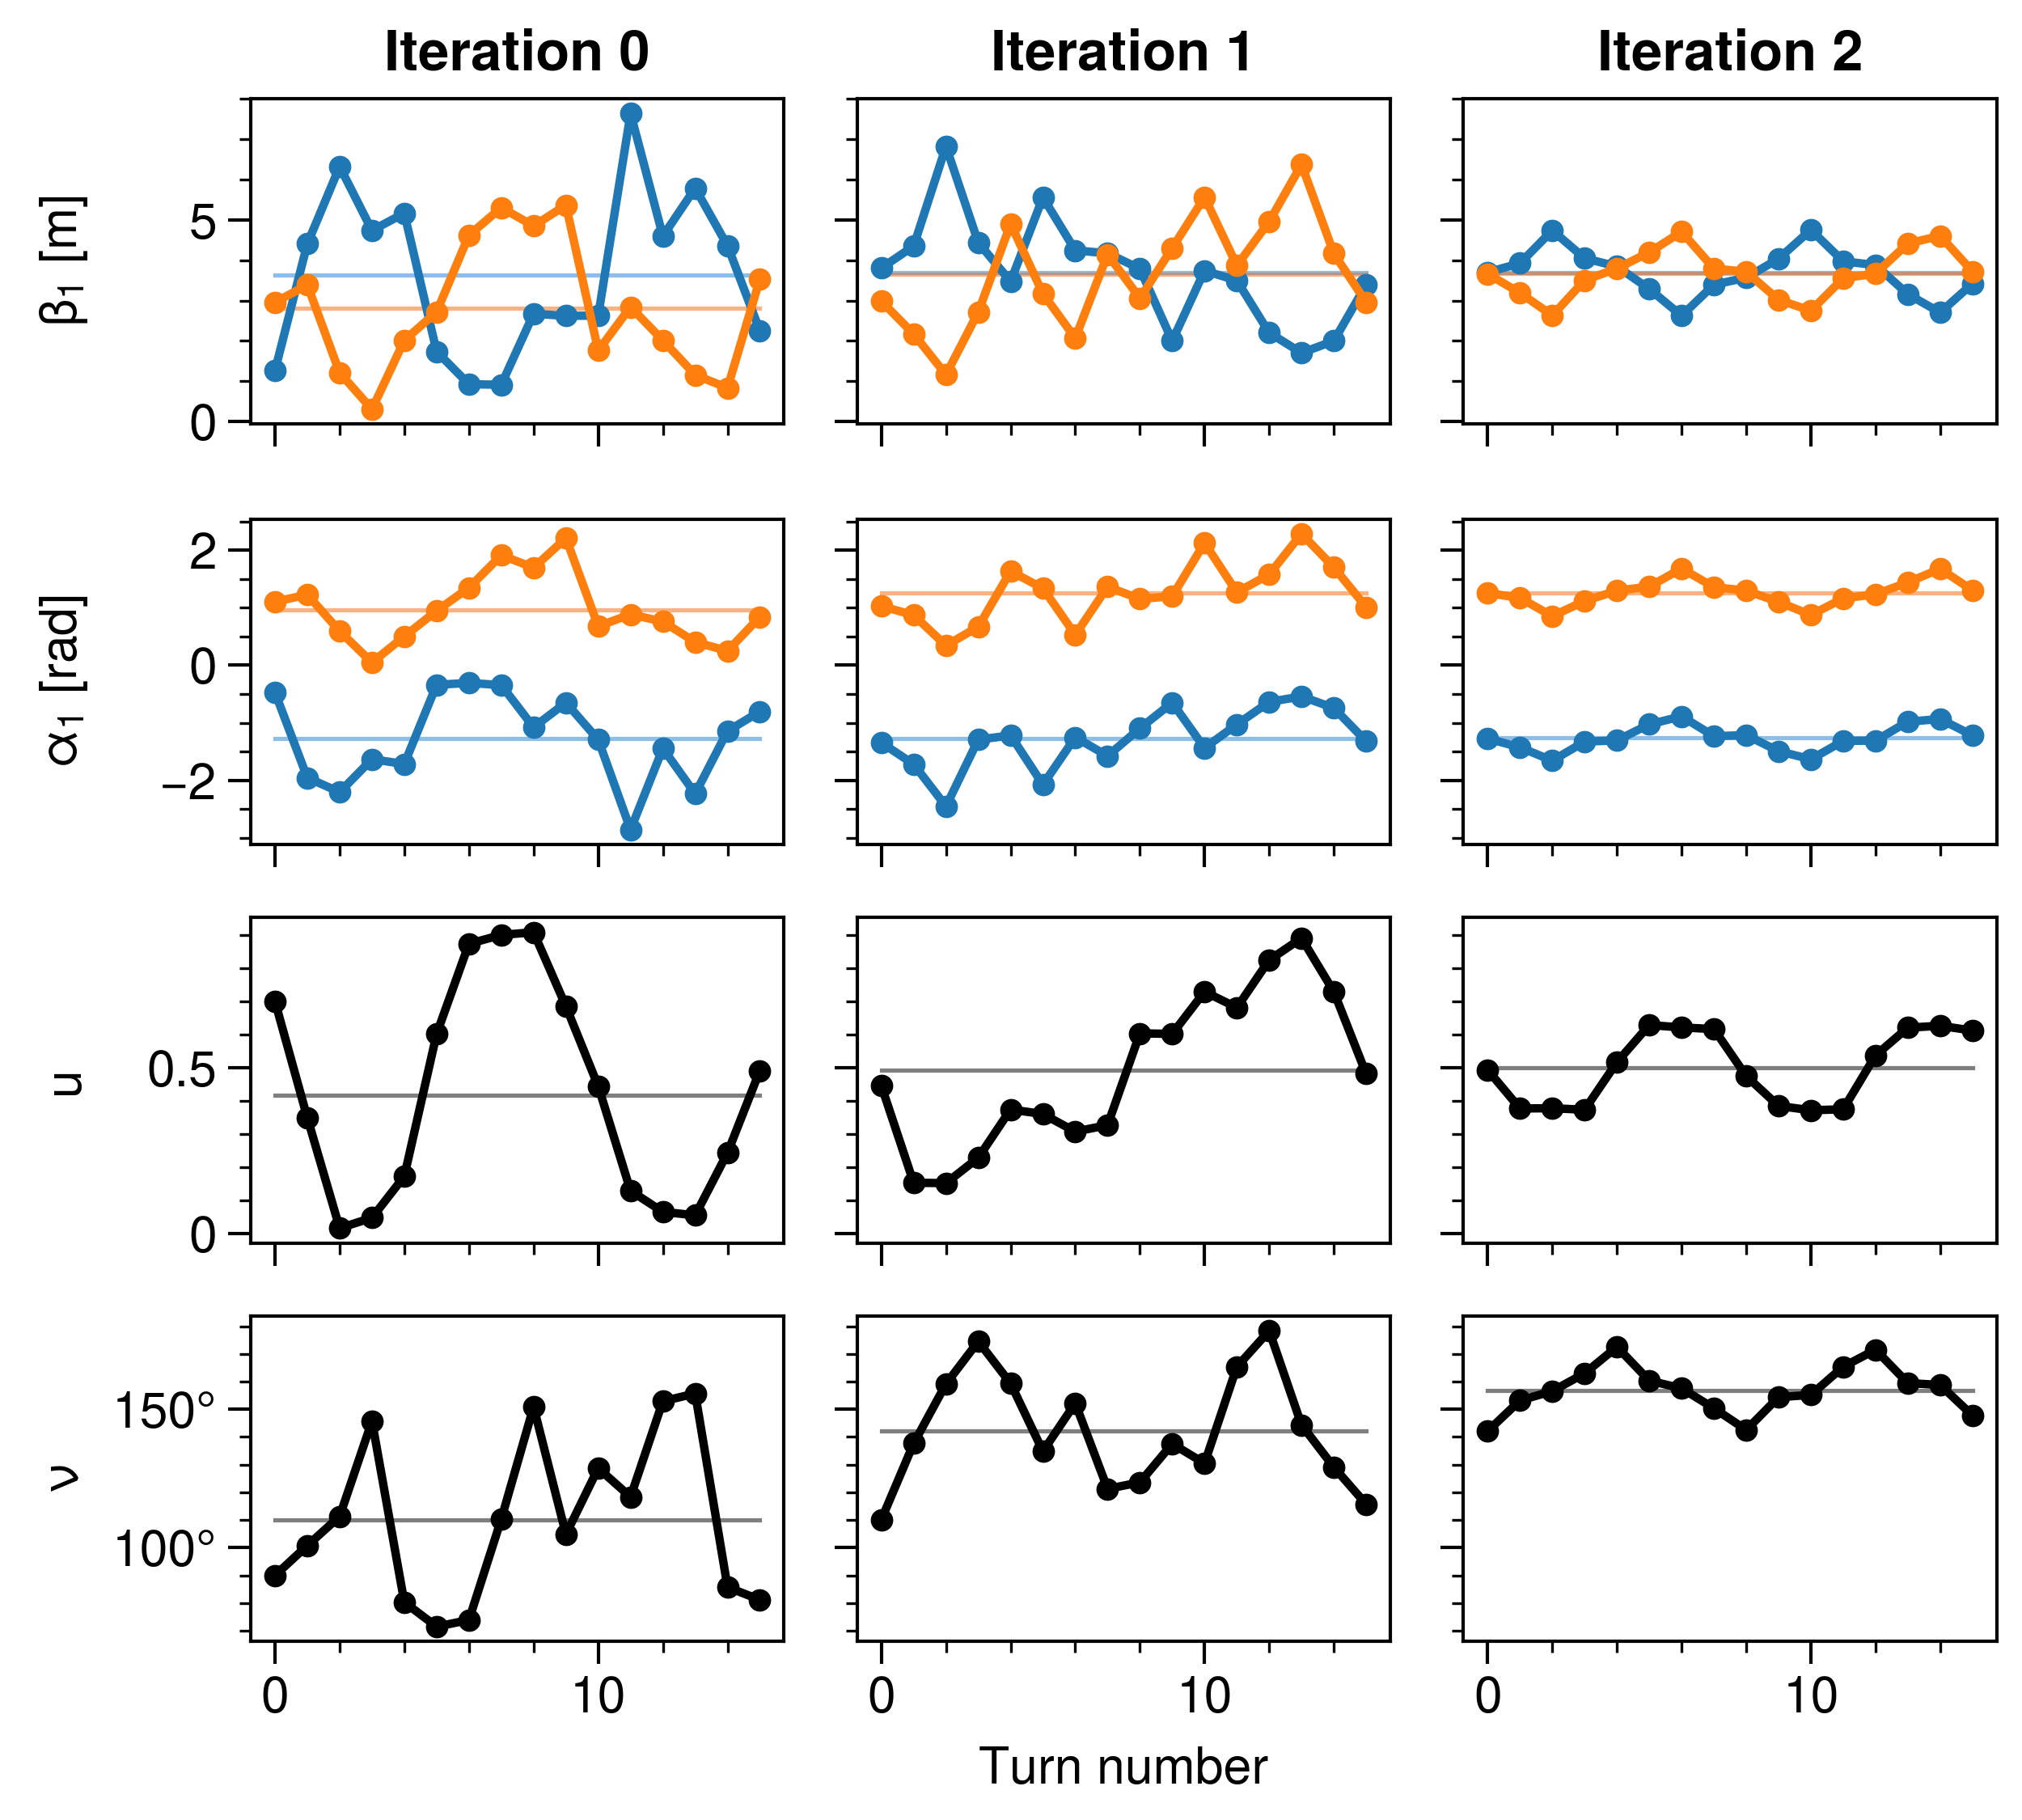
\includegraphics[width=0.8\textwidth]{Images/chapter2/optimizer_iters.png}
    \caption{Turn-by-turn oscillations of the beam parameters after the first few iterations of the matching routine. The custom update method is used. Faint horizontal lines give the average of the oscillations. Blue (orange) corresponds to $x$ ($y$).}
    \label{fig:optimizer_iters}
\end{figure}








\subsection{Method demonstration}

The matching routine was applied to an equally spaced, periodic quadrupole (FODO) lattice. The horizontal focusing strength in this lattice is shown in Fig.~\ref{fig:fodo_lattices}a as a function of $s$. Several variants of the FODO lattice were also considered to include external coupling: in Fig.~\ref{fig:fodo_lattices}b, the focusing and defocusing quadrupoles are rotated by $3\degree$ in opposite directions in the transverse plane, and in Fig.~\ref{fig:fodo_lattices}c solenoid magnets are inserted in the drift spaces between the quadrupoles. This section examines the matched solutions in each lattice as space charge is increased. Previous studies indicate that the KV envelope equations have a unique matched solution for each choice of lattice, beam perveance, and apparent emittances. Although there is no known proof of this conjecture, it seems to be true based on numerical evidence \cite{Lund2006}. Thus, for the Danilov distribution, it was expected that each choice of lattice and beam perveance would lead to two matched solutions depending on which intrinsic emittance is set to zero. No evidence to the contrary was found.
%
\begin{figure}[!p]
    \centering
    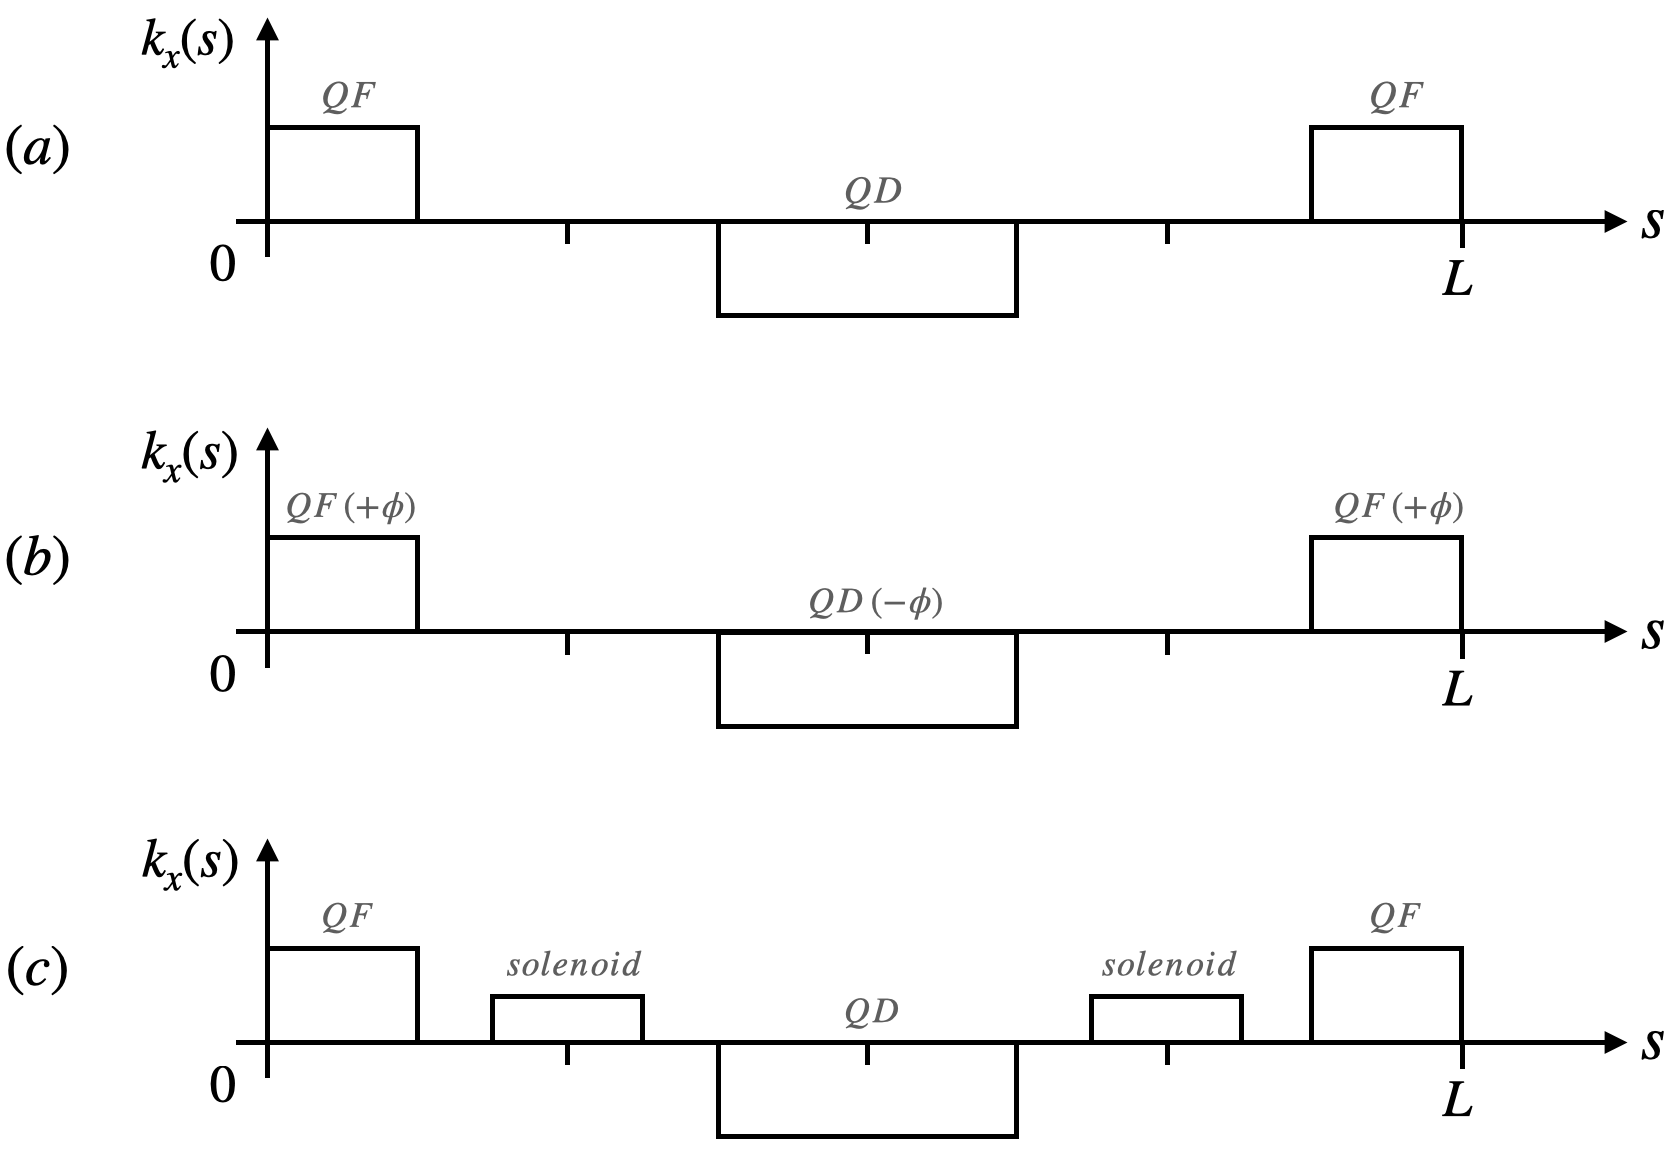
\includegraphics[width=0.9\textwidth]{Images/chapter2/fodo_lattices.png}
    \caption{Horizontal focusing strength as a function of $s$ in a FODO lattice with period length $L$. Quadrupoles have length $L/4$ and are equally spaced. (a) Upright quadrupoles with $80\degree$ phase advance in both planes. (b) The quadrupoles are rotated by $\phi = 3\degree$ in the transverse plane ($QF$ and $QD$ are rotated in opposite directions). (c) Solenoid magnets are inserted between the quadrupoles in (a).}
    \label{fig:fodo_lattices}
\end{figure}


\subsubsection{Uncoupled lattice}

We now apply the matching routine to an uncoupled FODO lattice. First, a note about the matched solution without space charge. The eigenvectors of the transfer matrix are uncoupled, meaning that $\mathbf{v}_1$ has no component in the $y$-$y'$ plane and $\mathbf{v}_2$ has no component in the $x$-$x'$ plane. A matched beam is formed by generating particles uniformly in phase along either of these eigenvectors; therefore, the matched beam is flat ($\varepsilon_x = 0$ or $\varepsilon_y = 0$). An exception occurs when the transfer matrix has degenerate eigenvalues, i.e., when the horizontal and vertical tunes are equal. In this case, any linear combination of eigenvectors forms another eigenvector. Thus, without space charge, there are an infinite number of matched solutions in a lattice with equal tunes. The free parameters from Eq.~\eqref{eq:twiss_params_4D} are $u$ and $\nu$.

We now include the self-force of the beam in the matching routine. Fig.~\ref{fig:matched_vs_sc_fodo} shows the matched beam sizes, apparent emittances, and $\nu$ parameter within the lattice for a range of linearly increasing space charge strengths.\footnote{For the zero space charge solution, we chose $u = 0.5$ and $\nu = \pi/2$.}
%
\begin{figure}[!p]
    \begin{subfigure}{1.0\textwidth}
        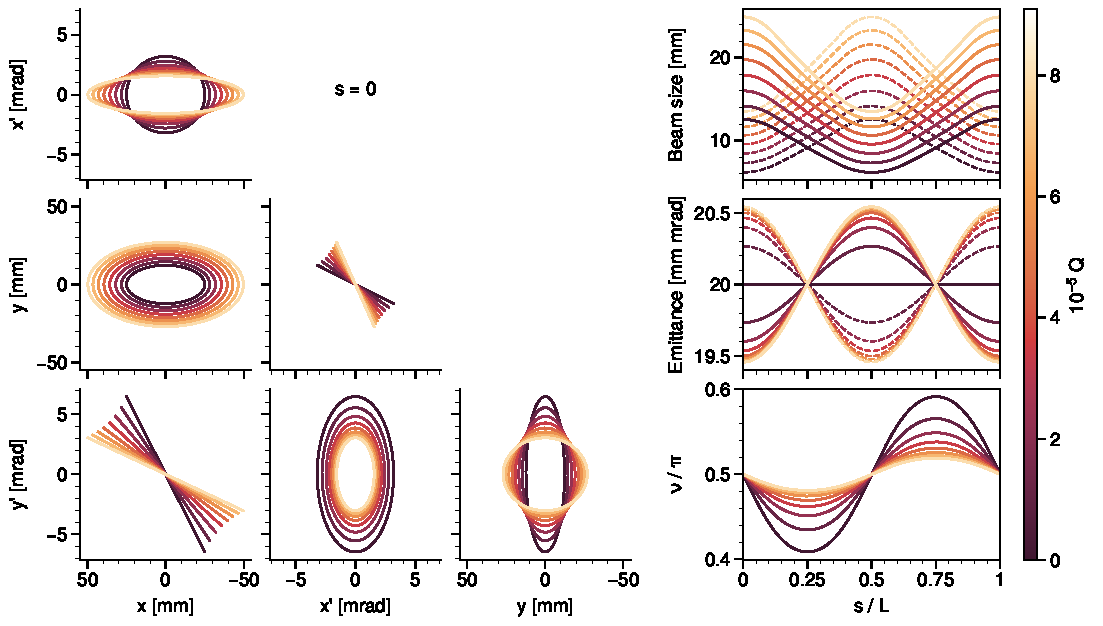
\includegraphics[width=\textwidth]{Images/chapter2/matched_vs_sc_fodo_mode1.pdf}
        \caption{Solution 1}
        \label{fig:matched_vs_sc_fodo_a}
    \end{subfigure}
    \vfill
    % \vspace*{1.0cm}
    \vfill
    \begin{subfigure}{1.0\textwidth}
        \centering
        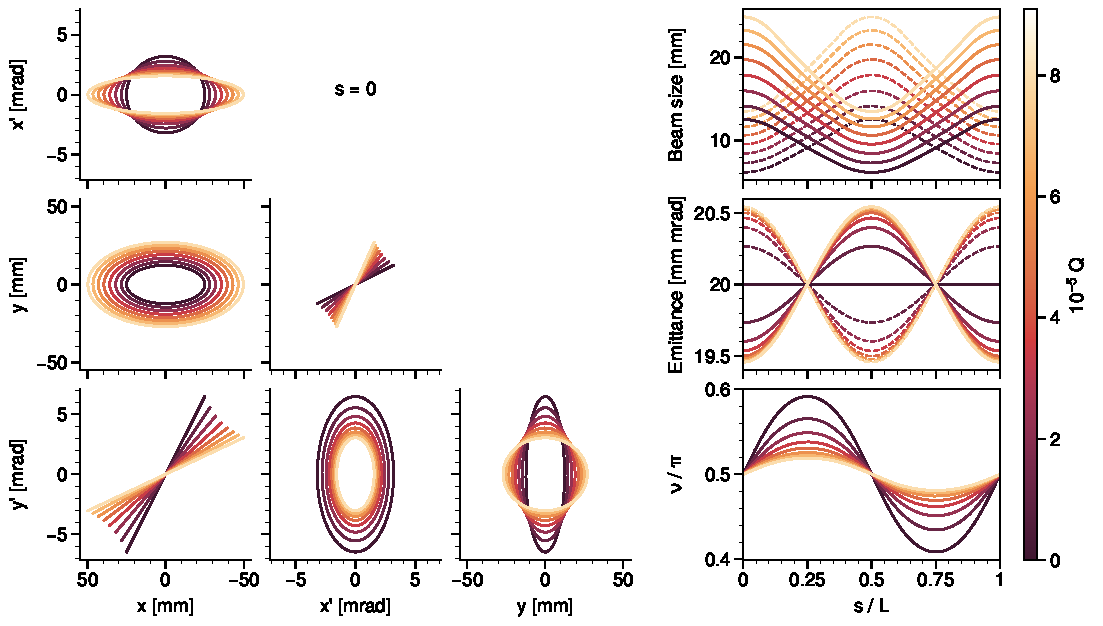
\includegraphics[width=\textwidth]{Images/chapter2/matched_vs_sc_fodo_mode2.pdf}
        \caption{Solution 2}
        \label{fig:matched_vs_sc_fodo_b}
    \end{subfigure}
    \caption{Matched envelope of the Danilov distribution in an uncoupled FODO lattice as space charge is increased. Left: phase space projections at the lattice entrance. Right: beam parameters within the lattice. Solid lines are for $x$ and dashed lines are for $y$ in the top two plots.}
    \label{fig:matched_vs_sc_fodo}
\end{figure}
%
It also shows the phase space projections at the lattice entrance. The following properties of the matched solutions are worth noting. First, except for the oscillatory apparent emittances, the beam evolution within the lattice when space charge is nonzero is very similar to the case of zero space charge. Second, two solutions are found which differ in the sign of their angular momentum. This is seen in the opposite signs of the slopes defining the linear relationships between the position in one plane and the momentum in the other; it is a consequence of the opposite directions of rotation of the two eigenvectors. The third property to note is how the solutions scale with increased space charge: the average width and height of the matched beam within the lattice grow approximately linearly, and the variation in the difference between the horizontal and vertical phase advances is suppressed — hence the decreased oscillation of the $\nu$ parameter. 

The same analysis can be performed when the horizontal and vertical tunes are split. We chose to increase the horizontal phase advance and decrease the vertical phase advance, both by $5\degree$. The results are displayed in Fig.~\ref{fig:matched_vs_sc_fodo_split}.\footnote{$\nu$ is undefined when the beam is flat, but we chose to draw a flat line at $\nu = \pi/2$.}
%
\begin{figure}[!p]
    \begin{subfigure}{1.0\textwidth}
        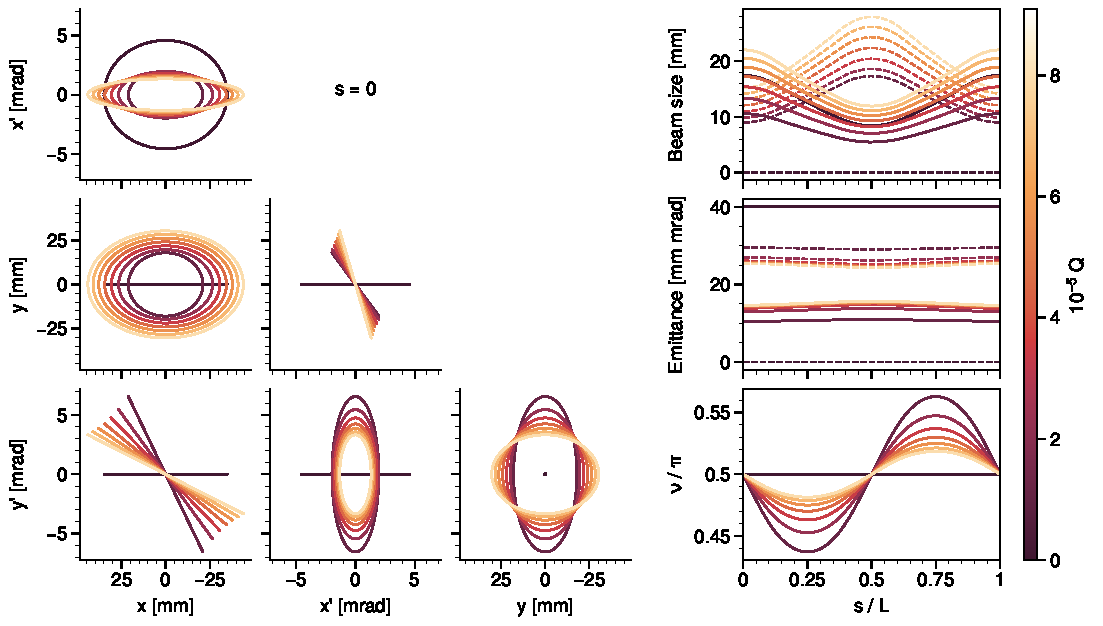
\includegraphics[width=\textwidth]{Images/chapter2/matched_vs_sc_fodo_split_mode1.pdf}
        \caption{Solution 1}
        \label{fig:matched_vs_sc_fodo_split_a}
    \end{subfigure}
    \vfill
    % \vspace*{1.0cm}
    \vfill
    \begin{subfigure}{1.0\textwidth}
        \centering
        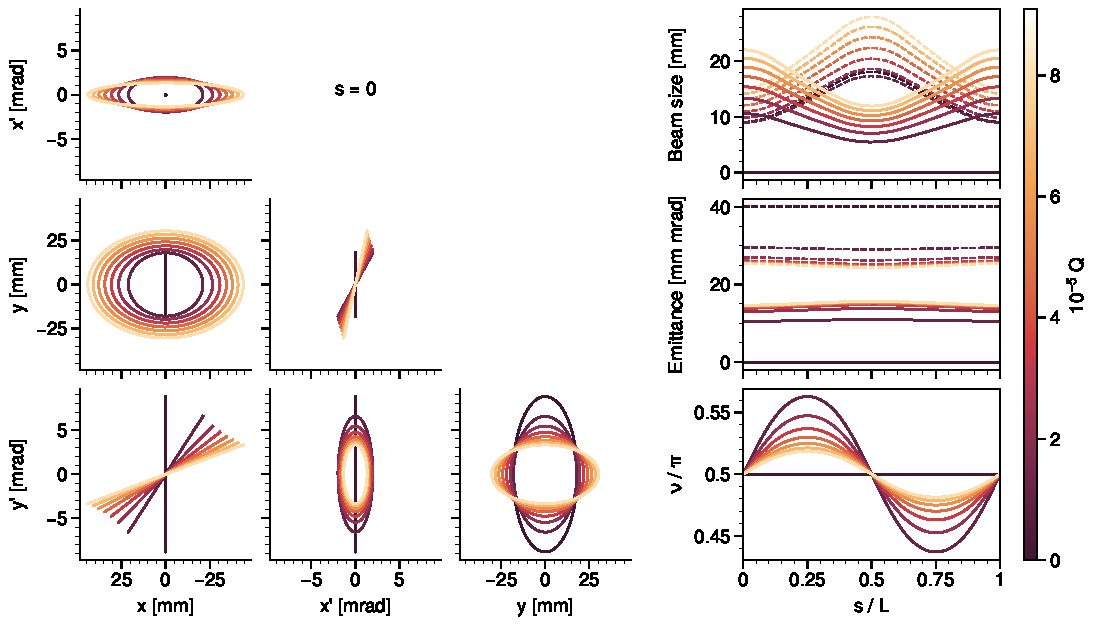
\includegraphics[width=\textwidth]{Images/chapter2/matched_vs_sc_fodo_split_mode2.pdf}
        \caption{Solution 2}
        \label{fig:matched_vs_sc_fodo_split_b}
    \end{subfigure}
    \caption{Matched envelope of the Danilov distribution in an uncoupled FODO lattice with unequal tunes as space charge is increased. Left: phase space projections at the lattice entrance. Right: beam parameters within the lattice. Solid lines are for $x$ and dashed lines are for $y$ in the top two plots.}
    \label{fig:matched_vs_sc_fodo_split}
\end{figure}
%
Due to the unequal tunes in the lattice, the zero space charge solution is flat, with maximal separation of the apparent emittances. Space charge generates a non-flat matched beam by decreasing the horizontal tune and increasing the vertical tune such that they are equal; for this reason, $\varepsilon_x < \varepsilon_y$ in every solution. The beam evolution within the lattice is similar to the previous case.


\subsubsection{Coupled lattice}

The same information as in Fig.~\ref{fig:matched_vs_sc_fodo} and Fig.~\ref{fig:matched_vs_sc_fodo_split} is plotted in Fig.~\ref{fig:matched_vs_sc_fodo_skew} for the skew quadrupole lattice from Fig.~\ref{fig:fodo_lattices}b.
%
\begin{figure}[!p]
    \begin{subfigure}{1.0\textwidth}
        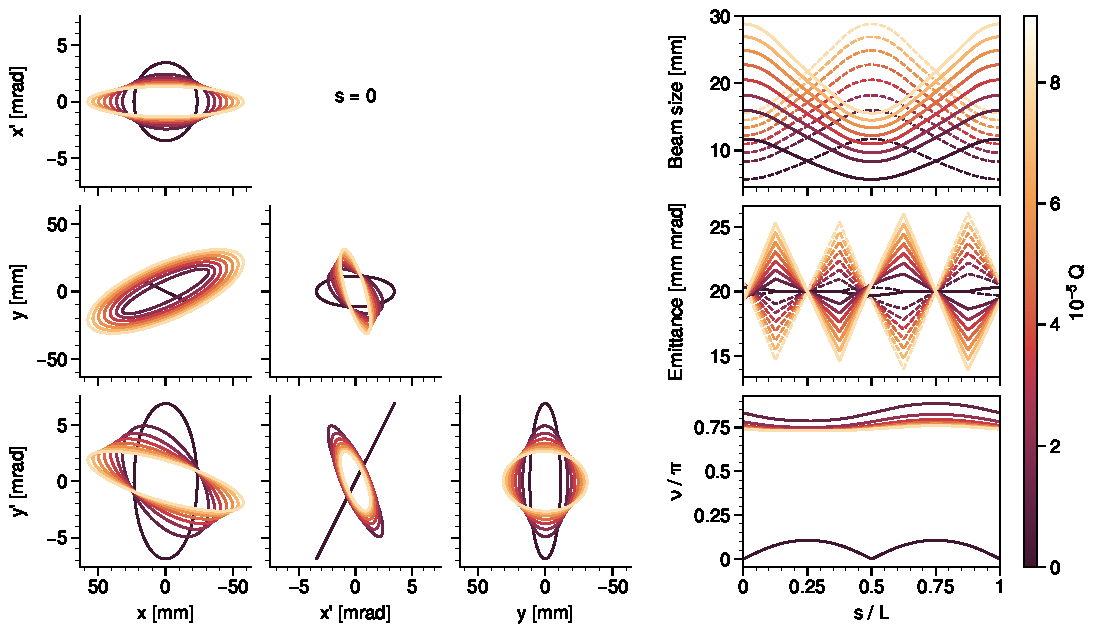
\includegraphics[width=\textwidth]{Images/chapter2/matched_vs_sc_fodo_skew_mode1.pdf}
        \caption{Solution 1}
        \label{fig:matched_vs_sc_fodo_skew_a}
    \end{subfigure}
    \vfill
    % \vspace*{1.0cm}
    \vfill
    \begin{subfigure}{1.0\textwidth}
        \centering
        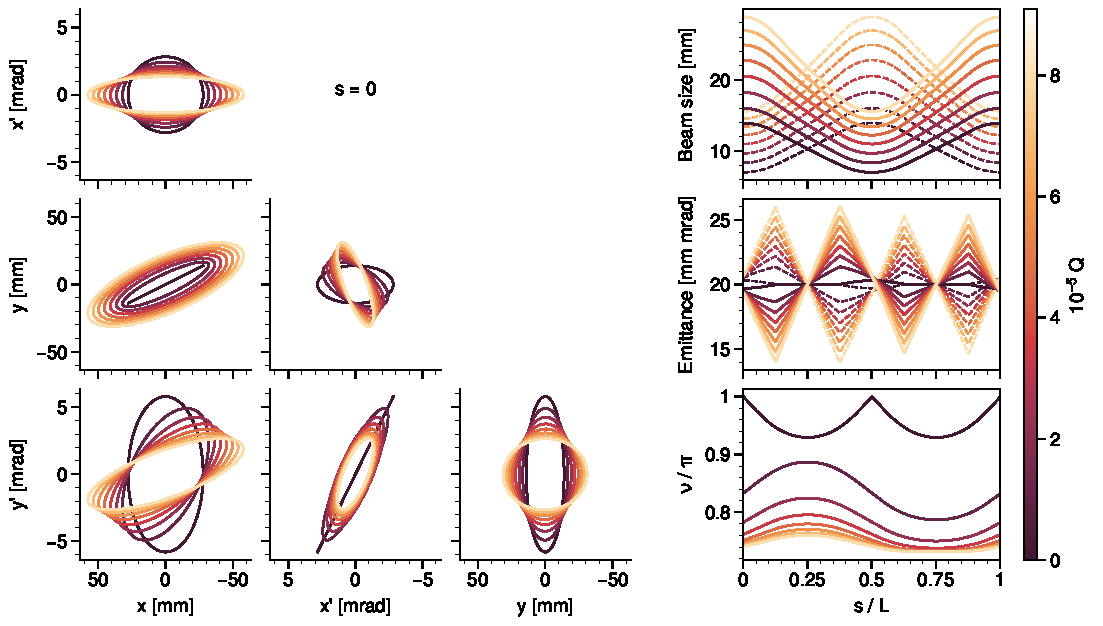
\includegraphics[width=\textwidth]{Images/chapter2/matched_vs_sc_fodo_skew_mode2.pdf}
        \caption{Solution 2}
        \label{fig:matched_vs_sc_fodo_skew_b}
    \end{subfigure}
    \caption{Matched envelope of the Danilov distribution in a coupled FODO lattice as space  charge is increased. The lattice is coupled due to skew quadrupoles. Left: phase space projections at the lattice entrance. Right: beam parameters within the lattice. Solid lines are for $x$ and dashed lines are for $y$ in the top two plots.}
    \label{fig:matched_vs_sc_fodo_skew}
\end{figure}
%
The locations of the skew quadrupoles are evident from the small arcs in the emittance curves. Without space charge, the matched beam at the center of the quadrupoles projects to a diagonal line in real space ($\nu = 0\degree$ or $180\degree$) with zero angular momentum, and the two solutions differ in the sign of the tilt angle of this line. The inclusion of space charge pulls $\nu$ away from these extreme values, resulting in a nonzero beam area. The cross-plane correlations between the positions and slopes also become nonzero, again revealing the opposite signs of the angular momentum between the two solutions. 

The presence of space charge leads to two solutions with the same tilt angle in the $x$-$y$ plane, as opposed to opposite tilt angles without space charge. This abrupt change in the matched beam orientation in solution 1 caused the optimizer to struggle for low space charge, often terminating due to a lack of progress. Fig.~\ref{fig:optimizer_comparison_a} shows the final cost as a function of the beam perveance, and Fig.~\ref{fig:optimizer_comparison_b} shows the turn-by-turn oscillations of the $\nu$ parameter for a subset of these cases. 
%
\begin{figure}[!p]
    \centering
    \begin{subfigure}{0.8\textwidth}
        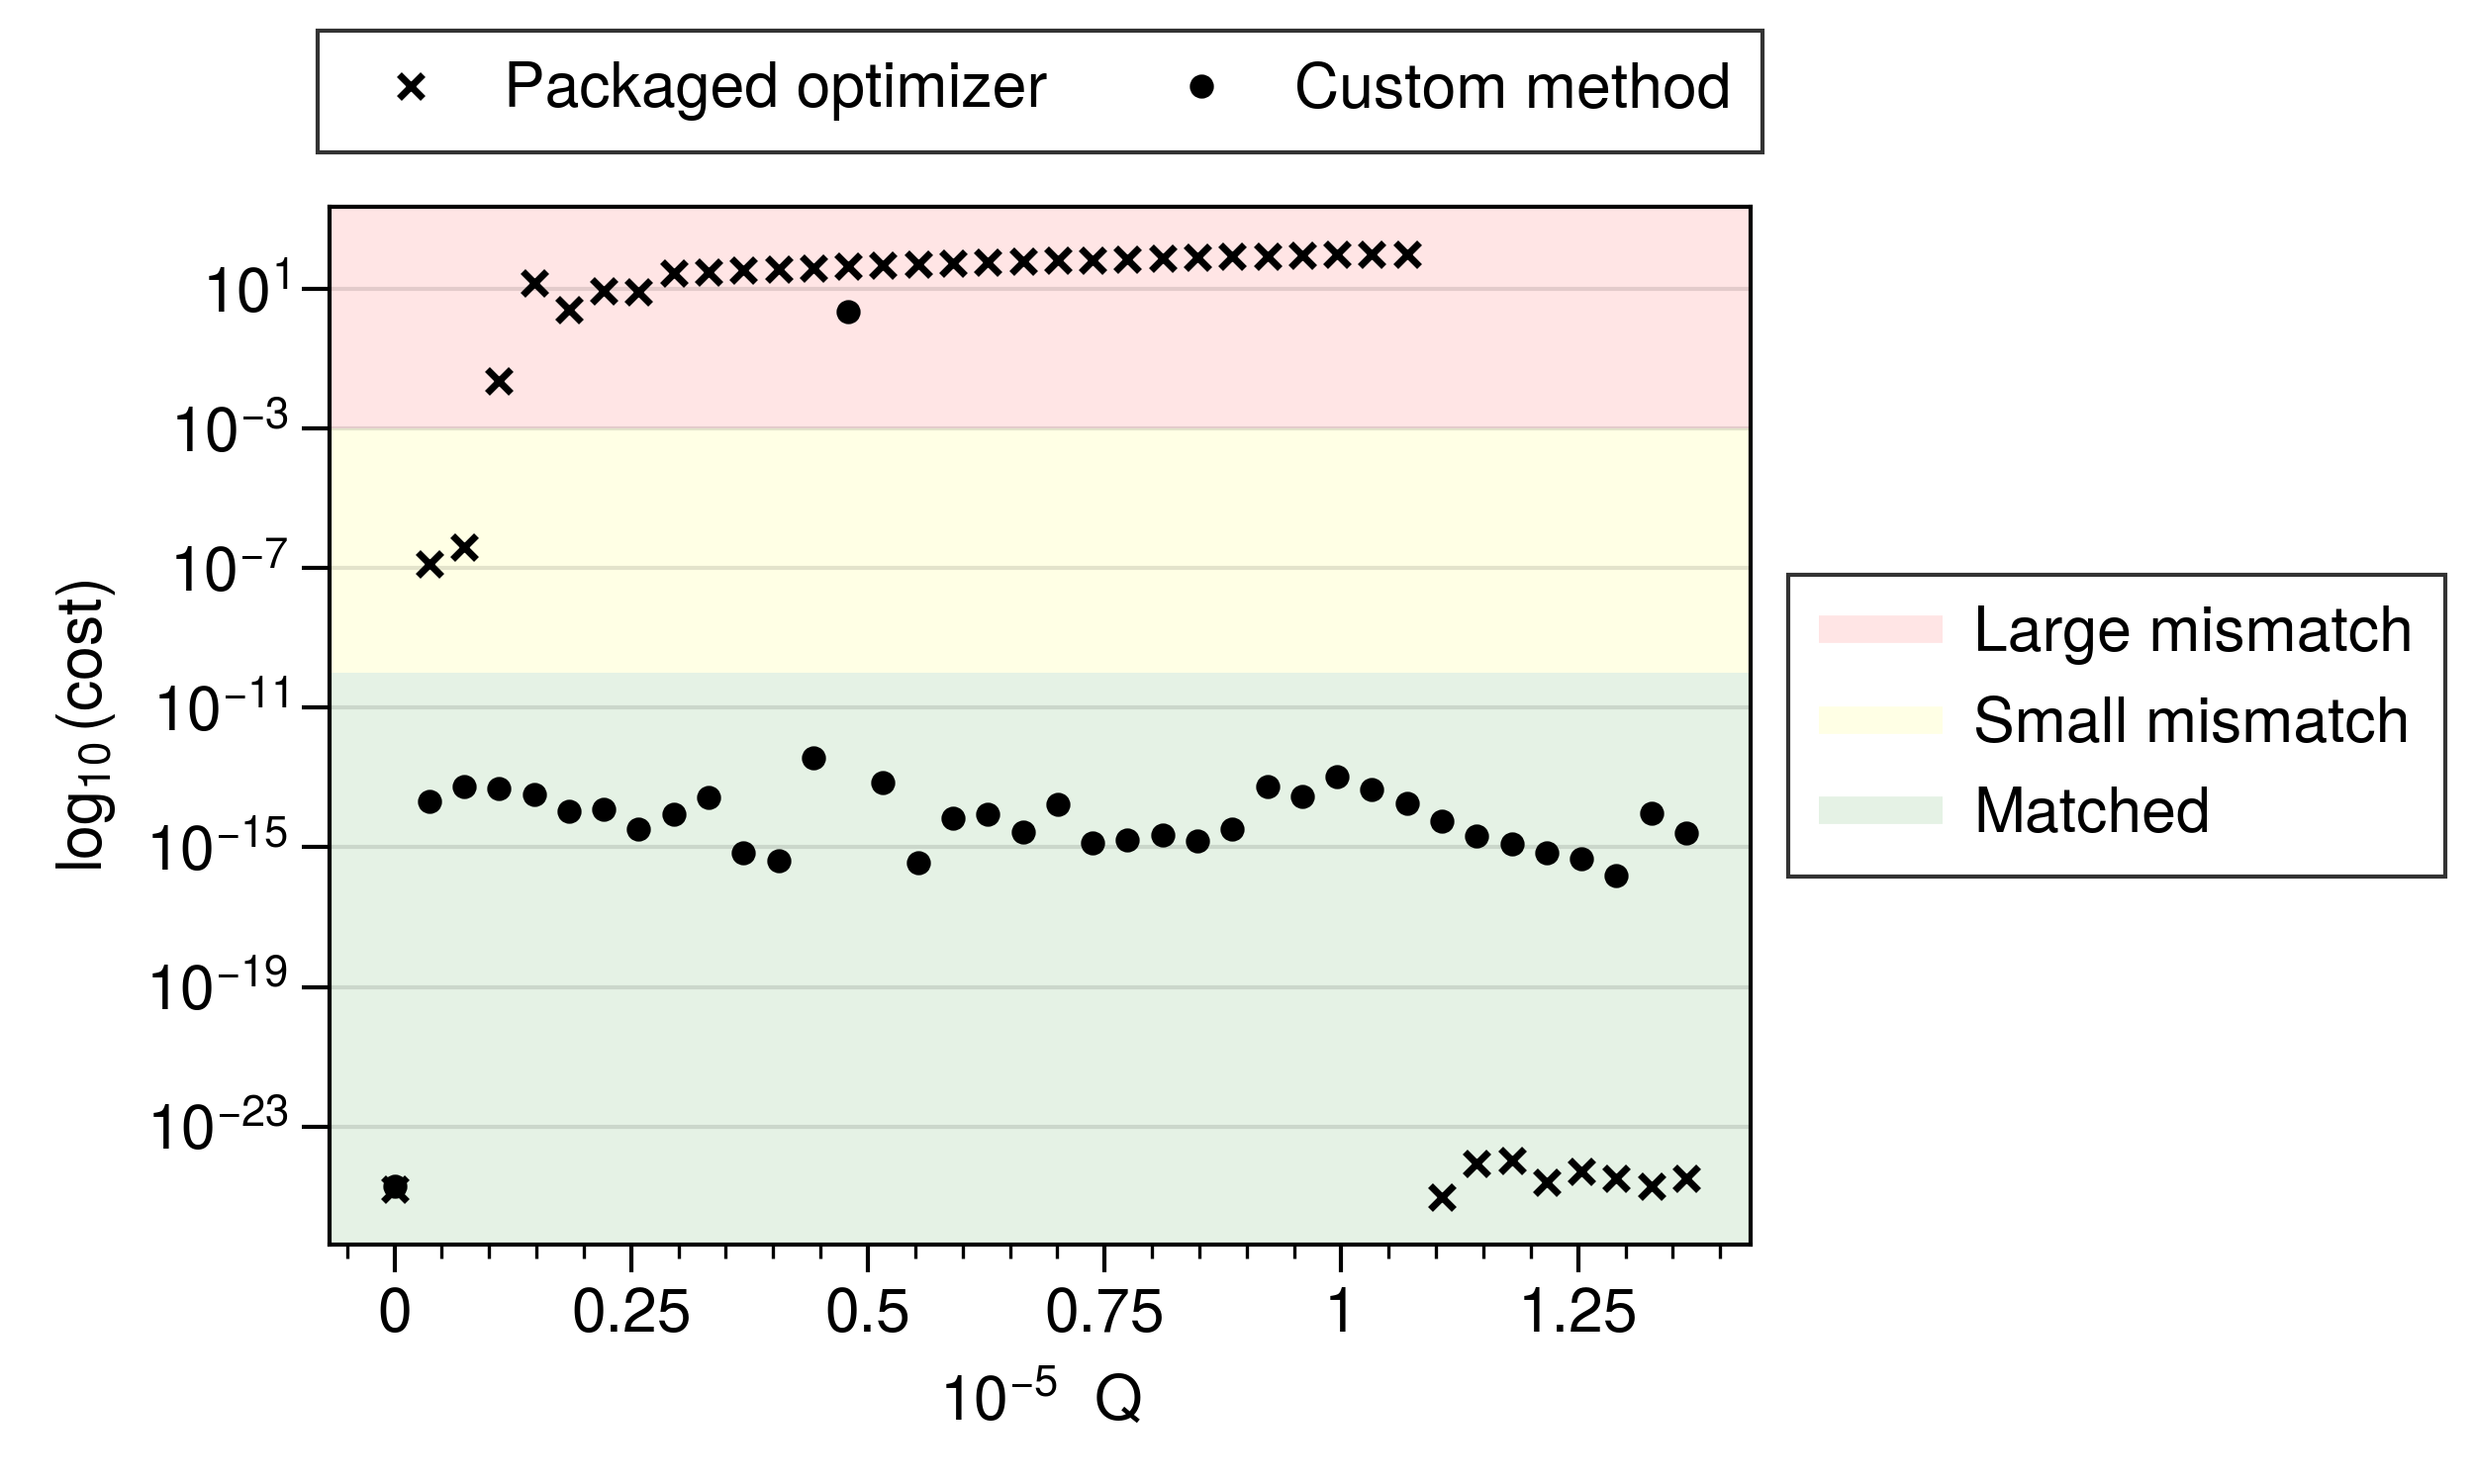
\includegraphics[width=\textwidth]{Images/chapter2/optimizer_comparison_costfunc.png}
        \caption{}
        \label{fig:optimizer_comparison_a}
    \end{subfigure}
    \vfill
    \vspace*{1cm}
    \vfill
    \begin{subfigure}{1.0\textwidth}
        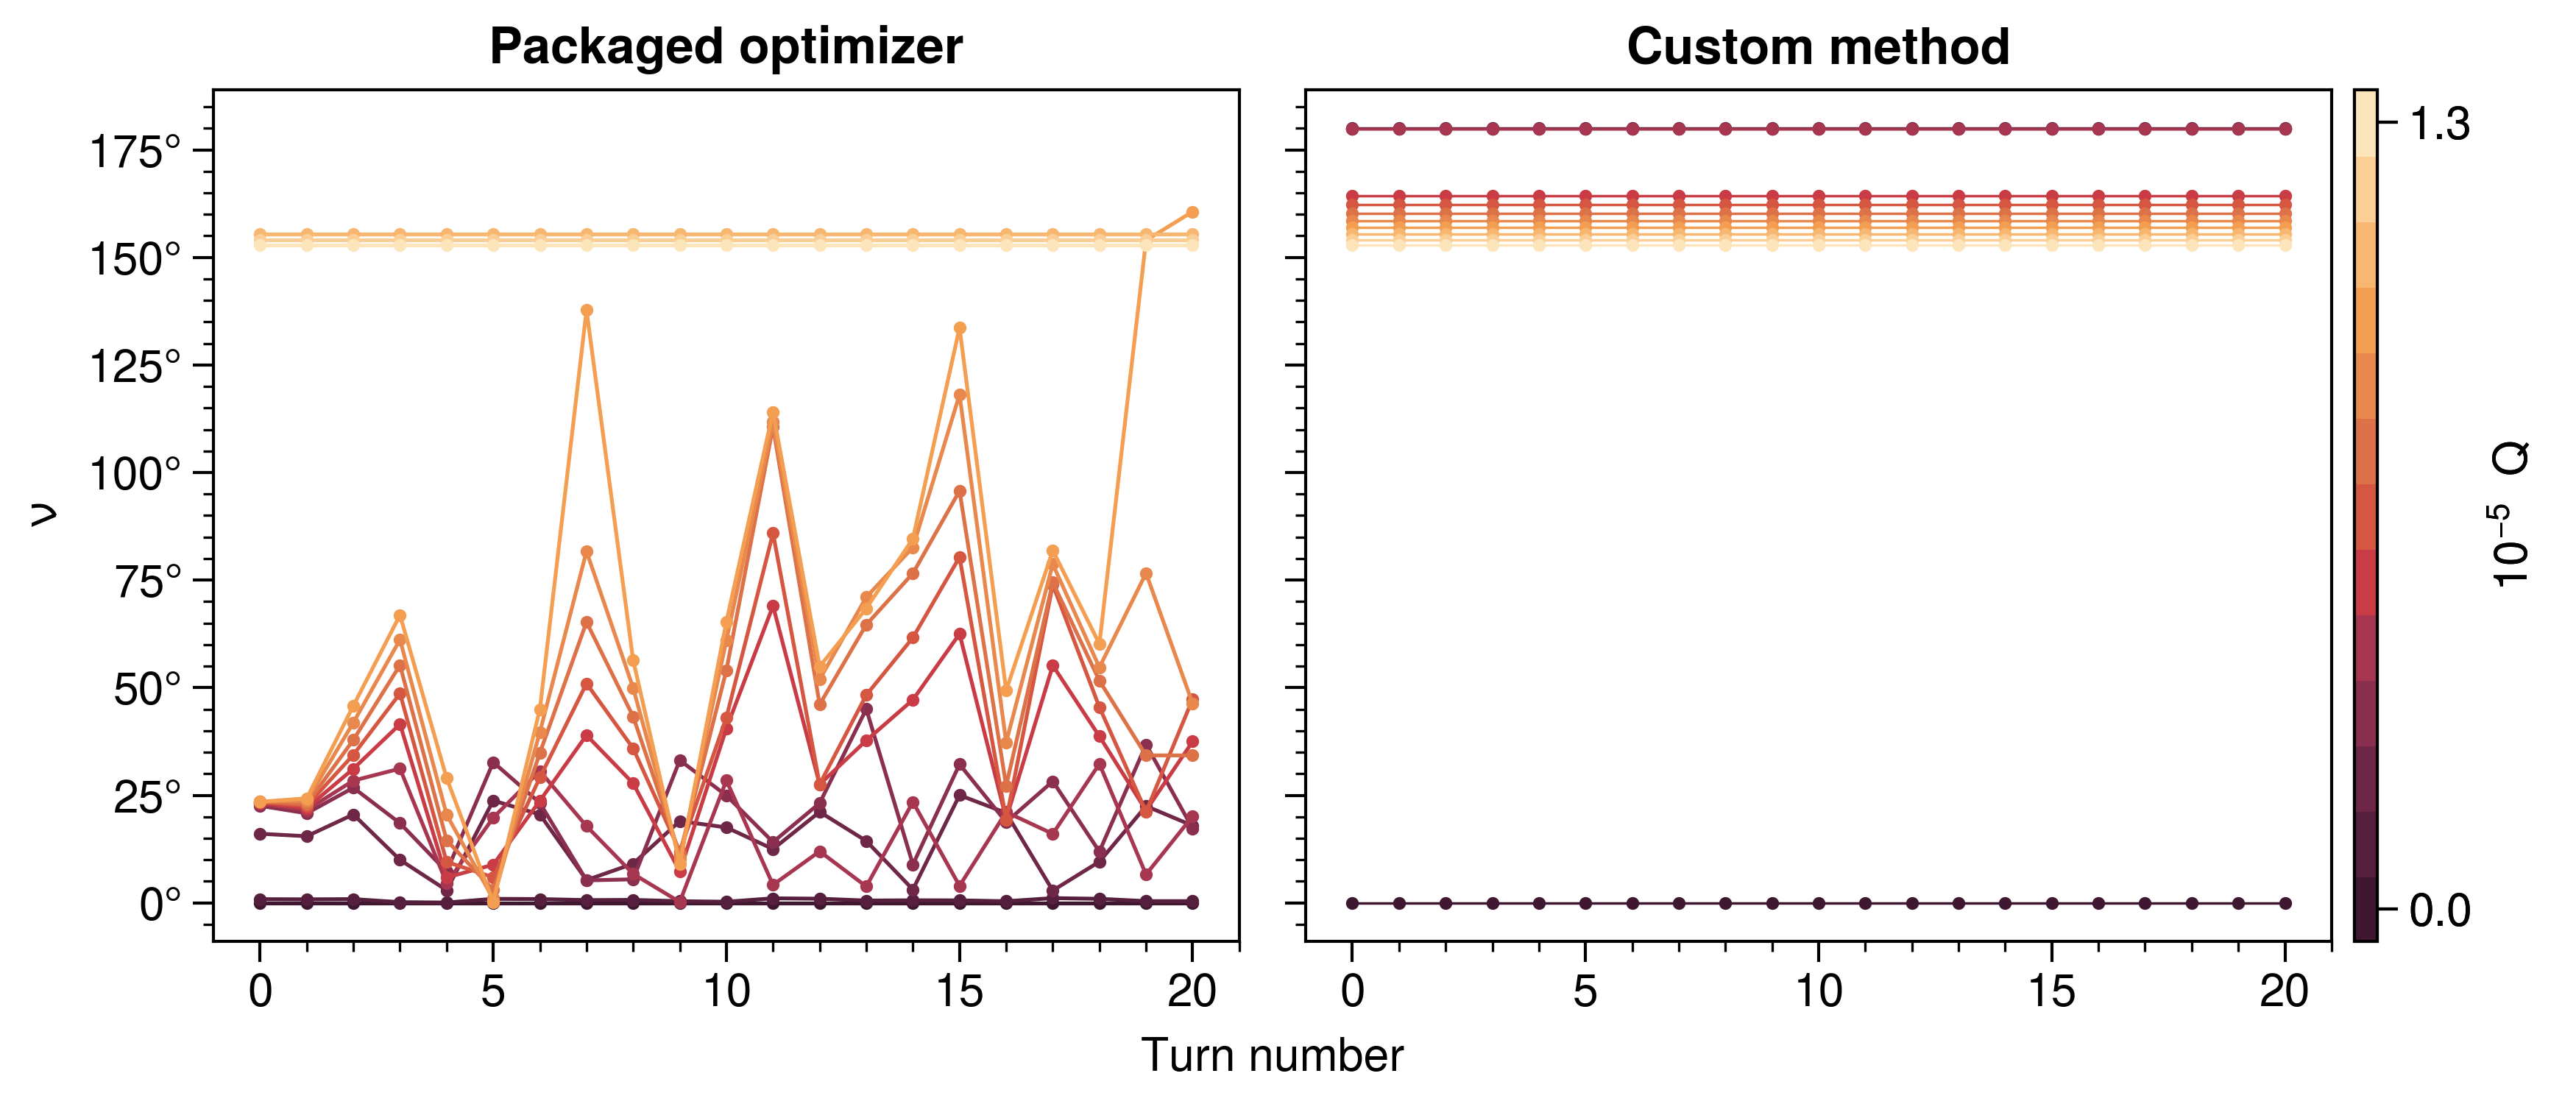
\includegraphics[width=\textwidth]{Images/chapter2/optimizer_comparison_tbt.png}
        \caption{}
        \label{fig:optimizer_comparison_b}
    \end{subfigure}
    \caption{Performance of the matching algorithm in a skew quadrupole lattice, corresponding to solution 1 in Fig.~\ref{fig:matched_vs_sc_fodo_skew_a}. (a) Final value of the cost function as a function of the beam perveance. (b) Turn-by-turn oscillations of the $\nu$ parameter after running each algorithm.}
    \label{fig:optimizer_comparison}
\end{figure}
%
The matching routine is not run when $Q = 0$ since the beam is already matched to the bare lattice; this corresponds to the bottom line in both panels of Fig.~\ref{fig:optimizer_comparison_b} at $\nu = 0$. The final cost is therefore the same for the two algorithms at this point. For small but nonzero perveance, the optimizer converges to a beam with $\nu \approx 0$ which exhibits very small mismatch oscillations (yellow region). The oscillations become more severe as the perveance is increased (red region), which corresponds to lines starting at $\nu \approx 25\degree$ in Fig.~\ref{fig:optimizer_comparison_b}. An exact match is eventually found (green region) when the perveance is sufficiently large with $\nu \approx 150\degree$. The averaging method, on the other hand, finds the exact match in nearly all cases. (Note that the circles and crosses on the far right of Fig.~\ref{fig:optimizer_comparison_b} represent the same beam; the algorithms have just terminated at different final costs.) This discussion simply illustrates that some care must be taken for certain values of the beam perveance when skew quadrupoles are present.

As a final demonstration of the method, coupling was included by the insertion of solenoid magnets in Fig.~\ref{fig:fodo_lattices}c. The results are shown in Fig.~\ref{fig:matched_vs_sc_fodo_sol}.
%
\begin{figure}[!p]
    \begin{subfigure}{1.0\textwidth}
        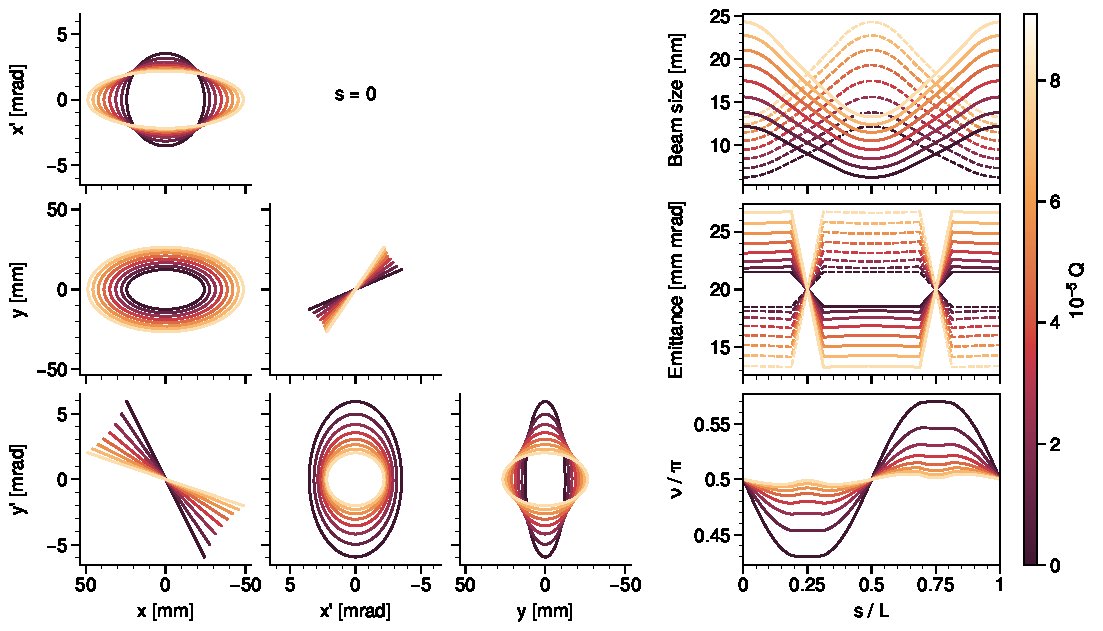
\includegraphics[width=\textwidth]{Images/chapter2/matched_vs_sc_fodo_sol_mode1.pdf}
        \caption{Solution 1}
        \label{fig:matched_vs_sc_fodo_sol_a}
    \end{subfigure}
    \vfill
    % \vspace*{1.0cm}
    \vfill
    \begin{subfigure}{1.0\textwidth}
        \centering
        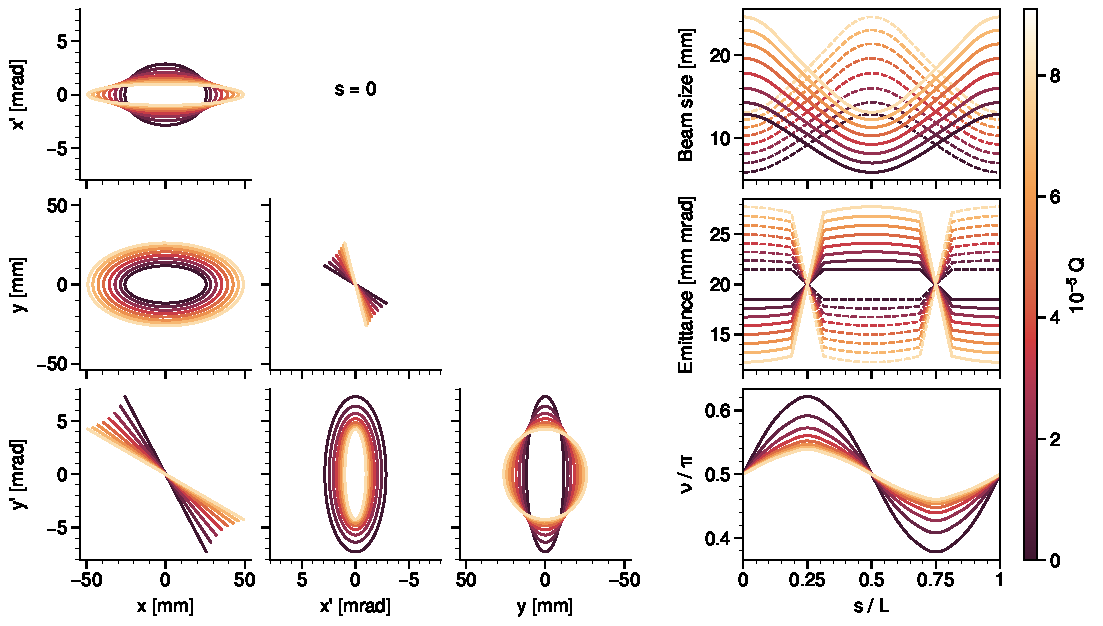
\includegraphics[width=\textwidth]{Images/chapter2/matched_vs_sc_fodo_sol_mode2.pdf}
        \caption{Solution 2}
        \label{fig:matched_vs_sc_fodo_sol_b}
    \end{subfigure}
    \caption{Matched envelope of the Danilov distribution in a coupled FODO lattice as space  charge is increased. The lattice is coupled due to solenoid magnets inserted between the quadrupoles. Left: phase space projections at the lattice entrance. Right: beam parameters within the lattice. Solid lines are for $x$ and dashed lines are for $y$ in the top two plots.}
    \label{fig:matched_vs_sc_fodo_sol}
\end{figure}
%
The matched beam resembles that of the uncoupled FODO lattice in Fig.~\ref{fig:matched_vs_sc_fodo}; most notably, it is round at the symmetry points in the lattice. The differences are found in the apparent emittances: their oscillation amplitude is larger within the drift spaces and quadrupoles, and there is a significant additional emittance exchange within the solenoids. 


\subsubsection{Effective transfer matrices}

The effective linear transfer matrix generated by the lattice and matched beam can be calculated by tracking test particles subject to the internal fields of the matched beam.\footnote{The matched beam is a function of one of the transfer matrix eigenvectors; the second eigenvector does not necessarily correspond to a matched solution in the same lattice. For example, the two solutions in the uncoupled FODO lattice share the same effective transfer matrix, but the two solutions in the skew quadrupole lattice do not share the same effective transfer matrix. In the latter case, the unused eigenvector is a matched solution in a lattice in which the sign of each skew term is reversed (a mirror reflection in one plane).} The eigenvalues of each effective transfer matrix are plotted in the complex plane as space charge is increased in Fig.~\ref{fig:effective_transfer_matrix_eigvals}.
%
\begin{figure}[!p]
    \centering
    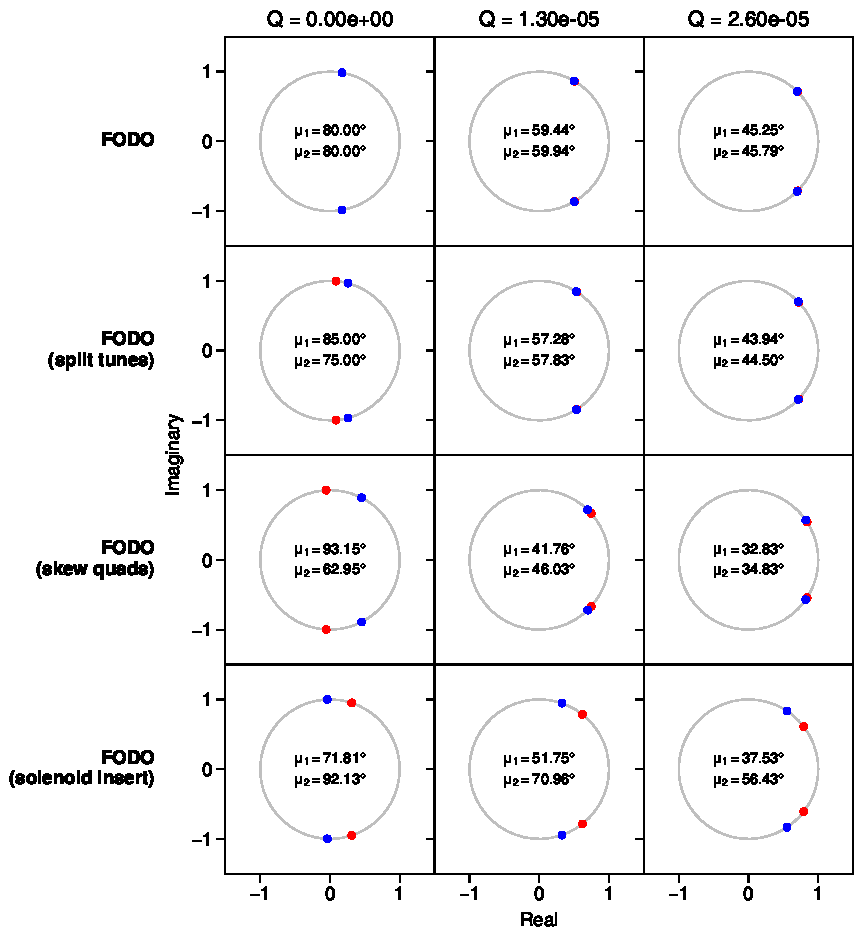
\includegraphics[width=\textwidth]{Images/chapter2/eigvals.pdf}
    \caption{Eigenvalues of the transfer matrix of the effective lattice generated by the matched beam, plotted in the complex plane.}
    \label{fig:effective_transfer_matrix_eigvals}
\end{figure}
%
We observe that the difference between the phase advances $\Delta = |\mu_2 - \mu_1|$, which is a measure of the coupling strength in the effective lattice, is never zero when space charge is nonzero. (In the top two rows, $\Delta$ is very small and the plotted eigenvalues lie nearly on top of one another.) We also observe that the matched beam space charge cancels out some of the bare lattice coupling; for example, in the skew quadrupole lattice, $\Delta$ is large in the left column but nearly zero in the right column. This is not true when coupling is included using solenoid magnets; $\Delta$ instead remains relatively constant.  


\section{Relevance to experiment}

These studies pave the way for future research on the stability of the Danilov distribution using perturbations around the matched envelope \cite{Goswami2016}, as well as halo formation using the particle-core model \cite{Wangler1998, Gluckstern1994, Gluckstern1998}. Our findings are also relevant to future experiments which will aim to produce an approximate Danilov distribution in the SNS ring using the elliptical painting method. Recall the definition of elliptical painting: the injection point is scaled along an eigenvector of the transfer matrix. It is critical to account for the beam's electric field when computing these eigenvectors; the painting must proceed along an eigenvector of the \textit{effective} transfer matrix generated by the matched beam.

The matching procedure was therefore applied to the SNS ring lattice. Using the simple focusing channels in the previous section, we found that the matched beam at a symmetry point ($\alpha_x = \alpha_y = 0$) in an uncoupled lattice tends to be upright ($\nu \approx \pi/2$); since the injection point in the SNS ring is close to a symmetry point, we expect this tendency to hold. The top row of Fig.~\ref{fig:matched_env_SNS} shows the matched envelope at the SNS injection point with realistic parameters: $\varepsilon_1 = 0$ mm~mrad, $\varepsilon_2 = 20$ mm~mrad, energy = 0.8 GeV, bunch length $\approx$ 3/4 ring length, intensity = $0.75 \times 10^{14}$, and equal tunes of 6.18.
%
\begin{figure}[!p]
    \centering
    \begin{subfigure}[t]{\textwidth}
        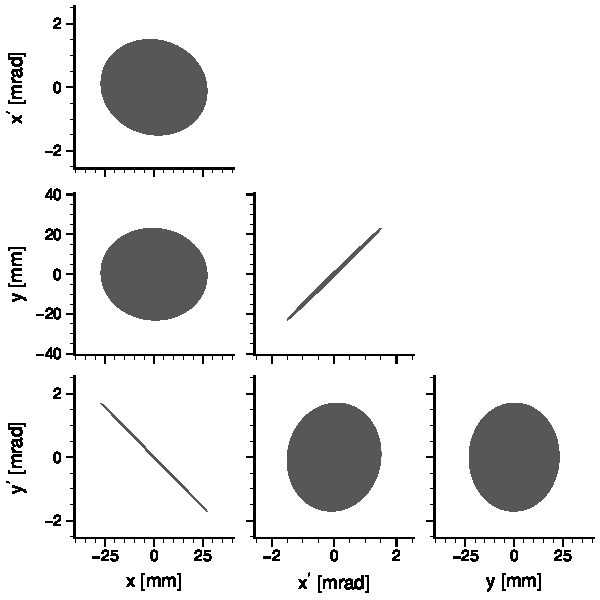
\includegraphics[width=0.65\textwidth, valign=t]{Images/chapter2/matched_env_SNS.pdf}
        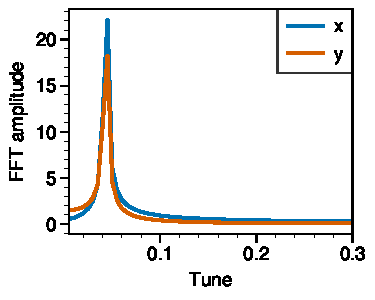
\includegraphics[width=0.33\textwidth, valign=t]{Images/chapter2/matched_env_SNS_fft.pdf}
    \end{subfigure}
    \vfill
    \vspace*{0.6cm}
    \vfill
    \begin{subfigure}[b]{\textwidth}
        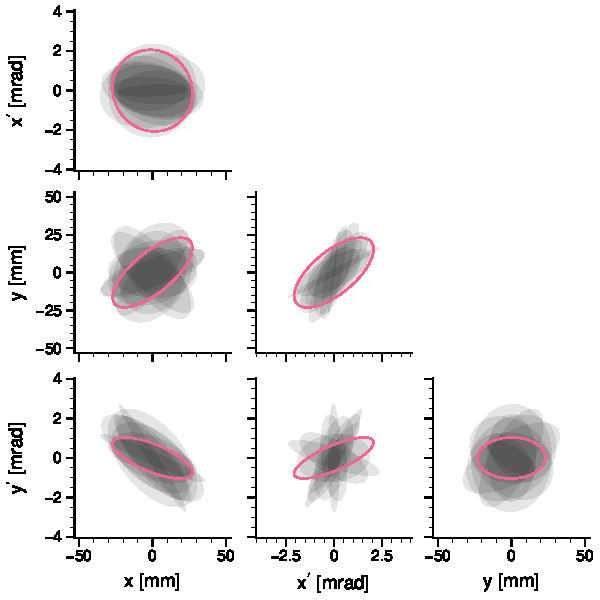
\includegraphics[width=0.65\textwidth, valign=t]{Images/chapter2/mismatched_env_SNS.pdf}
        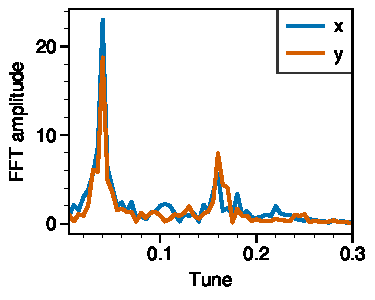
\includegraphics[width=0.33\textwidth, valign=t]{Images/chapter2/mismatched_env_SNS_fft.pdf}
    \end{subfigure}
    \caption{Matched (top) and mismatched (bottom) envelopes at the SNS ring injection point.}
    \label{fig:matched_env_SNS}
\end{figure}
%
The matched cross-plane parameters are $u \equiv \varepsilon_x / \varepsilon_2 \approx 0.5$ and $\nu \approx \pi / 2$. The FFT of the turn-by-turn oscillations of a particle on the edge of the beam over 200 turns is included on the right side of the figure, which shows that the tunes are equal. A mismatched initial beam is shown in the bottom row of Fig.~\ref{fig:matched_env_SNS}. The initial beam envelope, represented by the pink ellipses, has $\nu = \pi / 4$ and $u = 0.7$, with all other beam parameters unchanged. The beam ellipses over the next ten turns in the ring are overlayed on the same plot. The second peak in the Fourier spectrum represents a fast space-charge-driven emittance exchange, manifesting in the turn-by-turn rotation of the beam in the $x$-$y$ plane. 

If we attempted to paint the beam represented by the pink ellipses, the final distribution would resemble the superposition of the beams represented by the grey ellipses. As revealed by the blurred $x$-$y'$ and $y$-$x'$ correlations, the superposition of these beams is not a self-consistent distribution. Additionally, notice that the superposition has approximately equal apparent emittances; we therefore expect that even if the chosen painting parameters \textit{should} produce a larger beam size in one plane, the final beam will be approximately round ($\varepsilon_x \approx \varepsilon_y$). Finally, a uniform density ellipse would not be maintained in this scenario because particles would not always be injected onto the beam edge. We conclude that the painting path should be a line in the $x$-$y'$ (or $y$-$x'$) plane and that $x_{max}$ and $y_{max}'$ (or $y_{max}$ and $x_{max}'$) should be chosen such that the apparent emittances are equal.

These calculations complement the work of Holmes et al. \cite{Holmes2018}, who used realistic injection simulations to determine the feasibility of elliptical painting in the SNS.\footnote{These simulations are described in more detail in Chapter \ref{chap-3}.} One of their findings was that the ideal painting path in the SNS is a line in the $x$-$y'$ plane. This conclusion was reached empirically: simulations were repeated as the difference between the horizontal/vertical phases of the injected particles was varied, effectively changing the intended $\nu$ parameter of the painted beam, and the fraction of lost particles was recorded in each case. The major driver of losses is the geometry of the injection region, which restricts $x_{max}'$. 

Another finding from \cite{Holmes2018} was that when a solenoid is added to an uncoupled lattice with tune split $\nu_x$ - $\nu_y$, the final beam quality is, to a degree, insensitive to the tune split. It was suggested that the beam adjusts its shape such that the depressed horizontal and vertical tunes are equal. Using the envelope model and a simple lattice, we have confirmed that such a process can occur by varying the ratio of apparent emittances. This may be a contributing factor to the simulated beam behavior. Another important factor to consider is that the transfer matrix of the ring with the solenoid produces two eigenvectors, each of which rotates in a circle in the $x$-$y$ plane at the injection point. This does not depend on the tune split in the original lattice and remains true when linear space charge forces are included in the transfer matrix.

The above analysis demonstrates that envelope tracking is a valuable tool for the purposes of this work. Its main function is to provide fast insights into beam behavior and place rough constraints on the experimental parameters. We note that there remain unexplored modifications to the ring that may improve the painting method, and that some of these modifications could be tested using envelope tracking; for example, perhaps skew quadrupole correctors could be used to change the shape of the matched beam such that the required angular kicks, which introduce technical challenges as well as opportunities for beam loss, are minimized. 


\section{Summary}

The evolution of the Danilov distribution is given by its envelope equations. An iterative procedure to calculate the matched envelope was developed by observing that the matched beam is a function of a single eigenvector of an unknown coupled transfer matrix. The method was demonstrated in a simple FODO lattice, which was then modified to study the effects of unequal tunes and linear coupling. Two matched solutions were obtained for each lattice and space charge strength. The primary difference between these solutions was the sign of their angular momentum. A common finding among nearly all the cases was that the shape of the matched beam in phase space remained approximately the same as space charge was increased; the main effect of space charge was to increase the average beam area within the lattice, as well as to introduce an exchange of the apparent emittances.

The matching routine was then applied to the SNS ring. We found that the variation of the cross-plane beam parameters can generate large cross-plane mismatch oscillations, making the elliptical painting method impossible. It is therefore critical to account for the electric field of the matched beam when determining the painting path. We found that the matched beam at the SNS injection point is round ($\varepsilon_x \approx = \varepsilon_y$) with a $\pi / 2$ difference between the horizontal and vertical particle phases, constraining the painting path to a line in the $x$-$y'$ plane. These findings complemented the work in \cite{Holmes2018}, where the $x$-$y'$ painting path was recommended for independent reasons.

\chapter{Simulations} \label{chap-3}

Holmes et al. recently performed PIC simulations in the original ORBIT code to determine the feasibility of elliptical painting in the SNS \cite{Holmes2018}. Their findings are reviewed in this chapter. Additionally, the simulations are extended in PyORBIT to include updated experimental constraints. First, the computational model is briefly described. 


\section{Computational model}

The PyORBIT code tracks a Bunch object containing the 6D phase space coordinates. The accelerator is modeled as a series of nodes, each of which modifies the phase space coordinates in some way. Following the TEAPOT approach [\ref{}], single particles are transported using symplectic maps derived from the Hamiltonian. Here, we briefly describe the approach to nonlinear magnetic fringe fields and collective effects. 

\subsection{Space charge}

A major component of beam physics simulations is the calculation of the space charge force. Direct Coloumb sums are currently infeasible. The Vlasov equation can be solved directly, but this is difficult in 2D and 3D. The particle-in-cell (PIC) method is a “best of both worlds” approach in which an $N$ particle bunch is represented by $M$ macroparticles, where $M \ll N$. The macroparticles are tracked according to Eq.~\eqref{eq:eom_with_spacecharge}. The electric field is obtained by solving Eq.~\eqref{eq:Poisson} on a grid. The key step is transforming between the discrete and continuous representation. The PIC loop is shown in Fig.~\ref{fig:pic_loop}. 
%
\begin{figure}[!p]
    \centering
    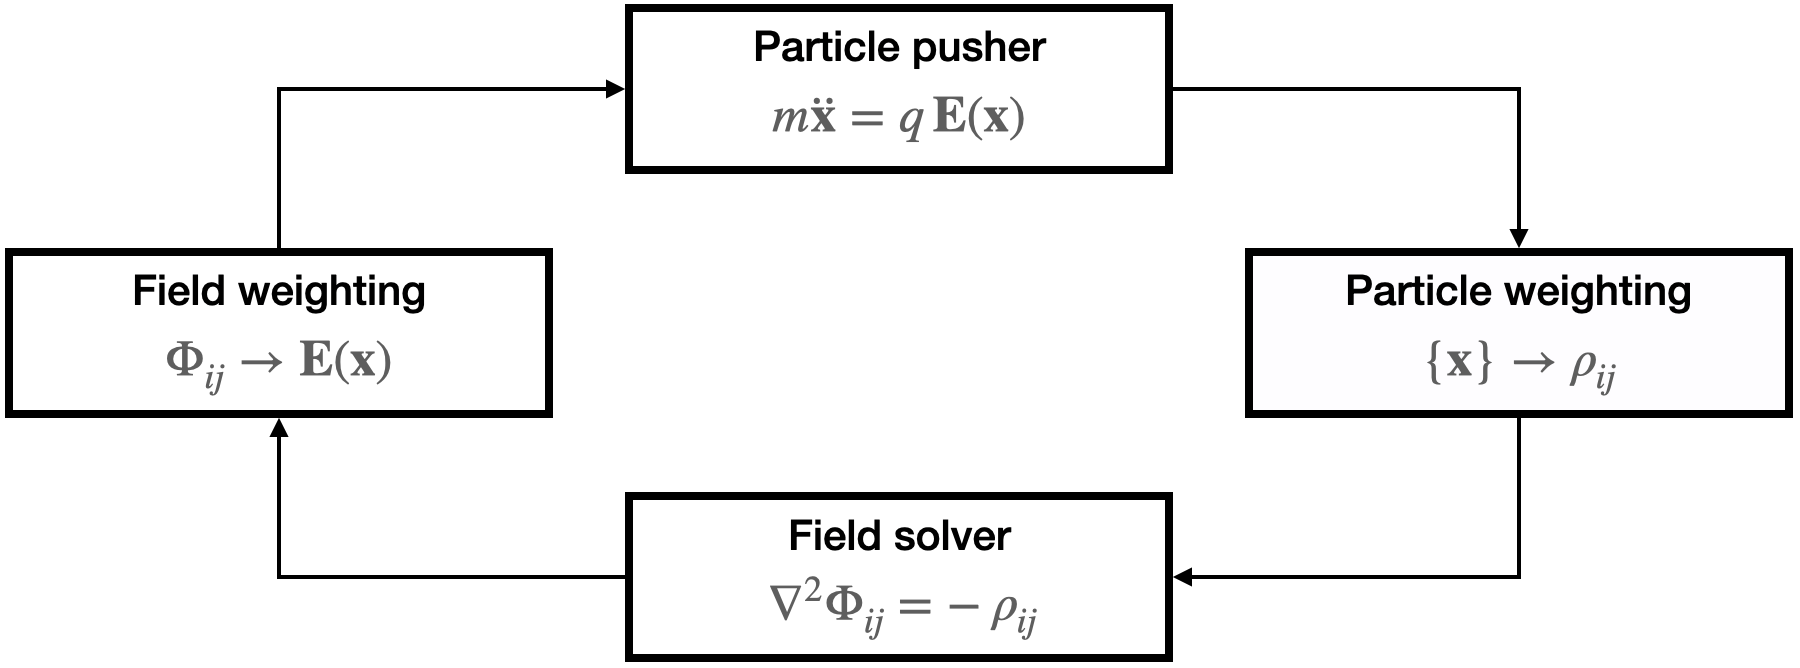
\includegraphics[width=\textwidth]{Images/chapter3/pic_loop.png}
    \caption{\label{fig:pic_loop}The particle-in-cell loop.}
    \vfill
    \vspace*{2.5cm}
    \vfill
    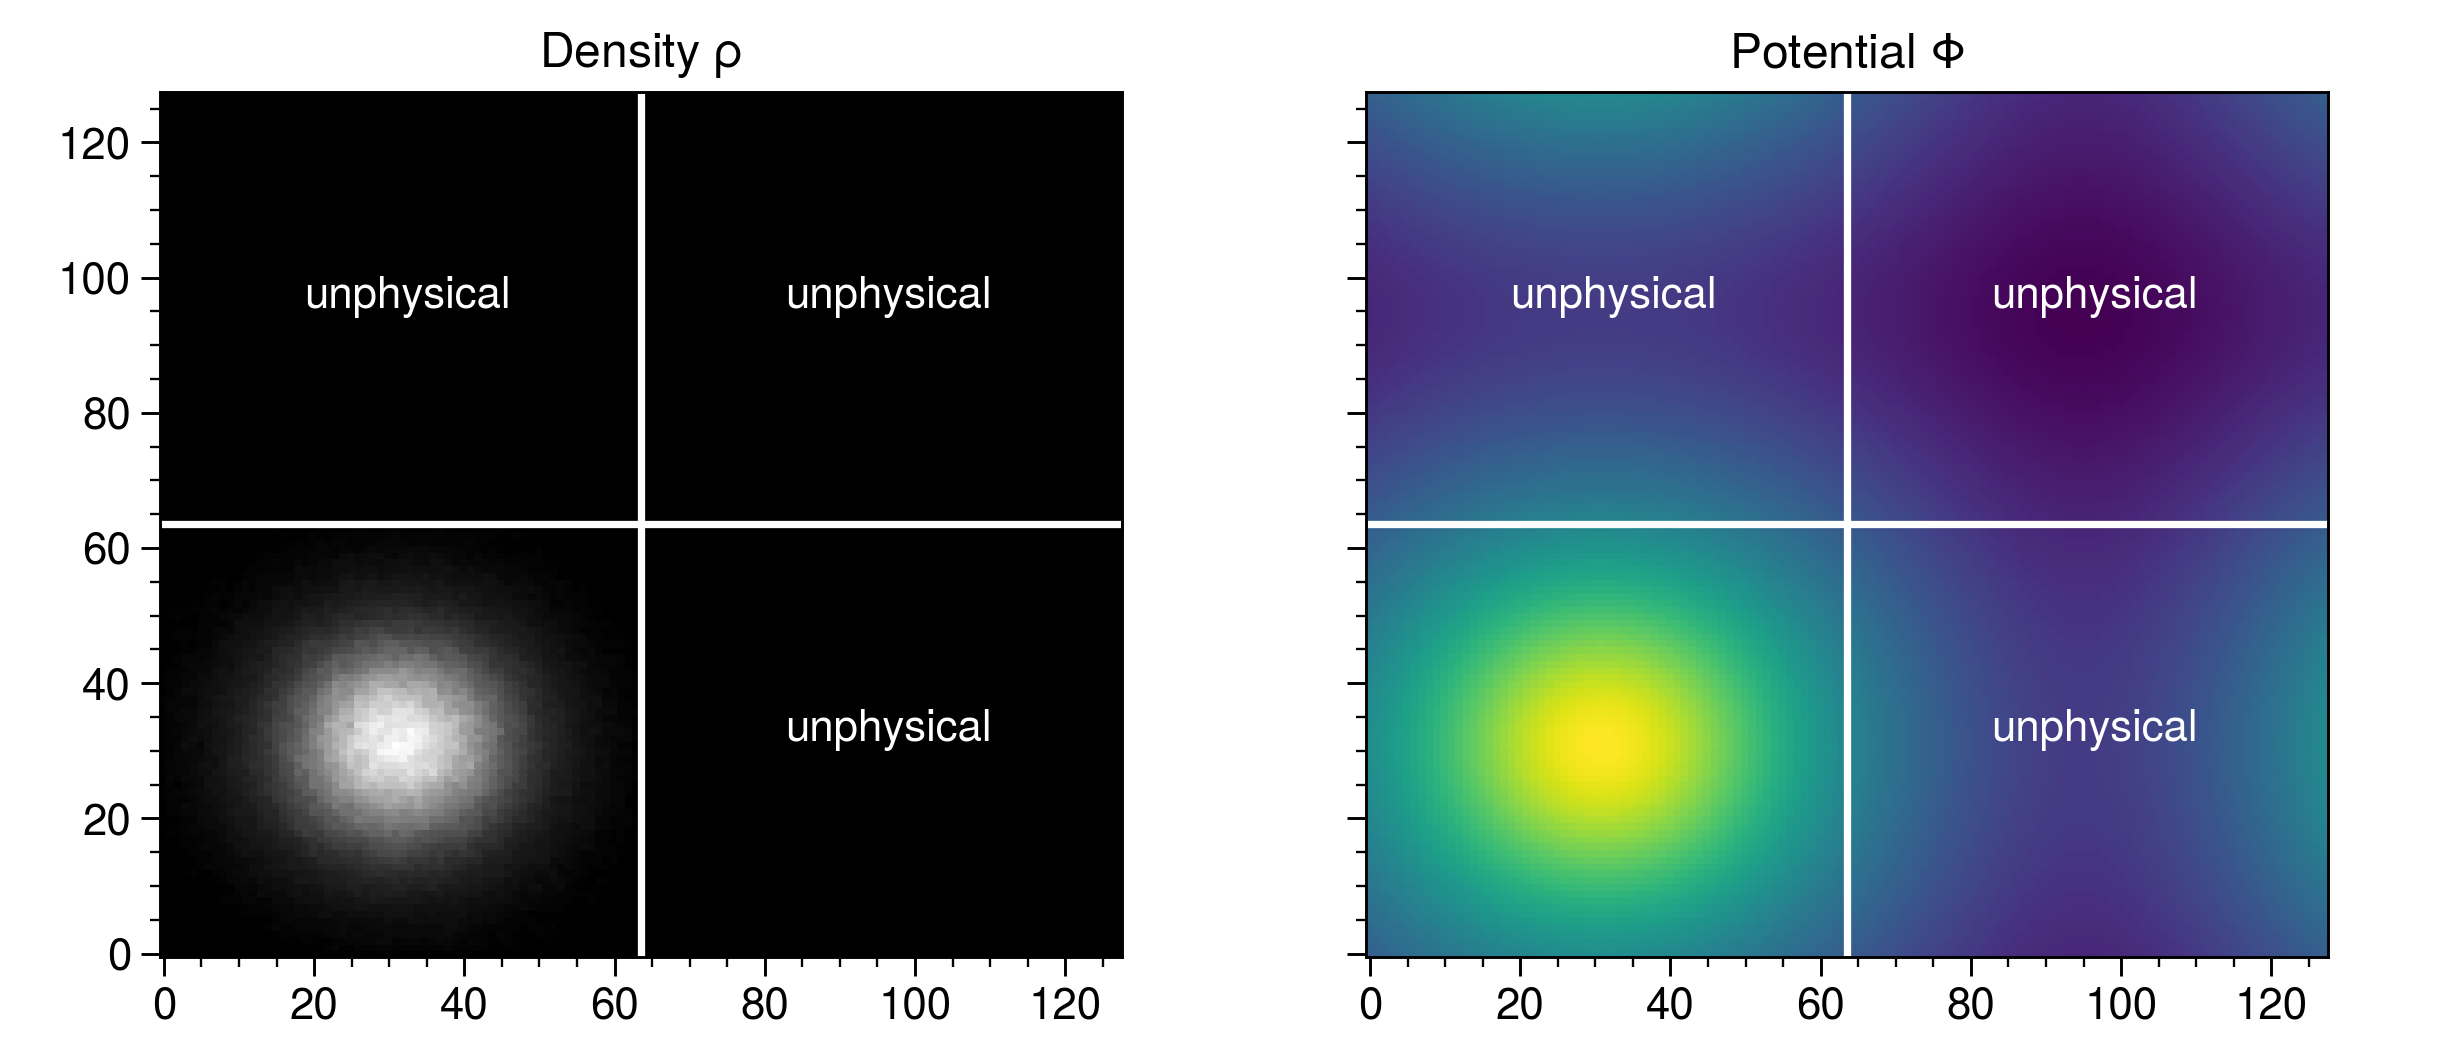
\includegraphics[width=\textwidth]{Images/chapter3/poisson.png}
    \caption{\label{fig:poisson}Solution of Poisson's equation on a doubled grid.}
    
\end{figure}
%

First, the charge density $\rho_{i,j}$ is obtained on a grid. A common method is to treat each macroparticle as a rectangular, uniform density cloud of charge with dimensions equal to the grid spacing, assigning a fractional charge to each bin according to the fraction of the cloud overlapping with that bin \cite{Birdsall1975}. Second, Poisson’s equation is solved on the grid. The method used in PyORBIT follows \cite{Hockney1981}. The potential is written as the convolution of a Green's function $G(\mathbf{x})$ with the charge density $\rho(\mathbf{x})$:
%
\begin{equation}
    \Phi(\mathbf{x}) = G(\mathbf{x}) * \rho(\mathbf{x}).
\end{equation}
%
We then exploit the convolution theorem \cite{Arfken1985} to write
%
\begin{equation}
    \mathcal{F}[\Phi(\mathbf{x})]
    =
    \mathcal{F}[G(\mathbf{x})] \cdot \mathcal{F}[\rho(\mathbf{x})]
\end{equation}
%
where $\mathcal{F}$ represents the Fourier transform. For a grid with $N$ bins per dimension, the time-complexity of the convolution is $O(N^2)$. The Fourier transform reduces this to $O(N \log N)$. To create periodic boundary conditions, the grid is doubled in each dimension. The Green's function is mirror-reflected onto these new regions, while the charge density is set to zero. The potential is solved for on the extended grid, after which the unphysical regions are discarded. An example is shown in Fig.~\ref{fig:poisson}. Third, using the same weighting method as the first step, the gradient of the potential is interpolated at the particle positions. Finally, the particle momenta are updated using an appropriate integration scheme.

Care must be taken when choosing the number of macroparticles, grid size, and integration step size. In the following simulations, 128 bins are used in each dimension. The number of macroparticles changes during injection, but the final number of particles is usually at least $3 \times 10^{5}$.

In rings where the coasting beam approximation is valid, the longitudinal and transverse dimensions are treated separately. In PyORBIT, a longitudinal space charge node acts on the bunch once per turn. Two models are included for the transverse space charge calculation: the 2.5D model and the sliced model. In the 2.5D model, Poisson’s equation is solved once for a charge density obtained by projecting the entire bunch onto the $x$-$y$ plane; the transverse space charge forces are then weighted according to the longitudinal density. In the sliced model, the bunch is longitudinally sliced, and Poisson’s equation is solved for each slice. 

\subsection{Wake fields}

In the discussion of space charge thus far, the beam was assumed to be in free space. In reality, the beam is in a conducting vacuum chamber. Charged particles leave so-called wake fields on the conducting surface, which then act on other particles or on the same particle in a ring, possibly leading to instability. The treatment of wake fields can be challenging and is introduced in \cite{Chao1993}. No details are described here; we just mention that PyORBIT takes these effects into account.


\subsection{Fringe fields}

Quadrupole, dipole, and solenoid magnets are finite in length; the magnetic fields outside the core are nonlinear. These are referred to as fringe fields. [...]


\subsection{Other effects}

An important effect during charge-exchange injection is Coulomb scattering during passage through the stripper foil. [...].

Finally, longitudinal focusing in the ring is provided by two RF cavities. The harmonic frequency $h$ is defined as the RF frequency divided by the revolution frequency of the beam; one cavity operates at $h = 1$ and the other operates at $h = 2$, both at an amplitude near 5 kV. The energy gain $\Delta \epsilon$ for a particle passing through the cavity is approximated as  
%
\begin{equation}
    \Delta \epsilon = q V \sin((h \phi + \phi_0).
\end{equation}
%
The particle phase $\phi$ is zero for the synchronous particle.



\section{Fringe field correction}

It was found in \cite{Holmes2018} that in an otherwise linear lattice, fringe fields tend to eliminate any cross-plane correlations in the beam when the tunes are near the difference resonance $\nu_x \approx \nu_y$. To demonstrate this, we generate a Danilov distribution matched to a linearized version of the SNS ring. Fringe fields are then turned on, and the particles are tracked without space charge. Fig.~\ref{fig:fringe} shows the turn-by-turn evolution.
%
\begin{figure}
    \centering
    \begin{subfigure}{0.7\textwidth}
        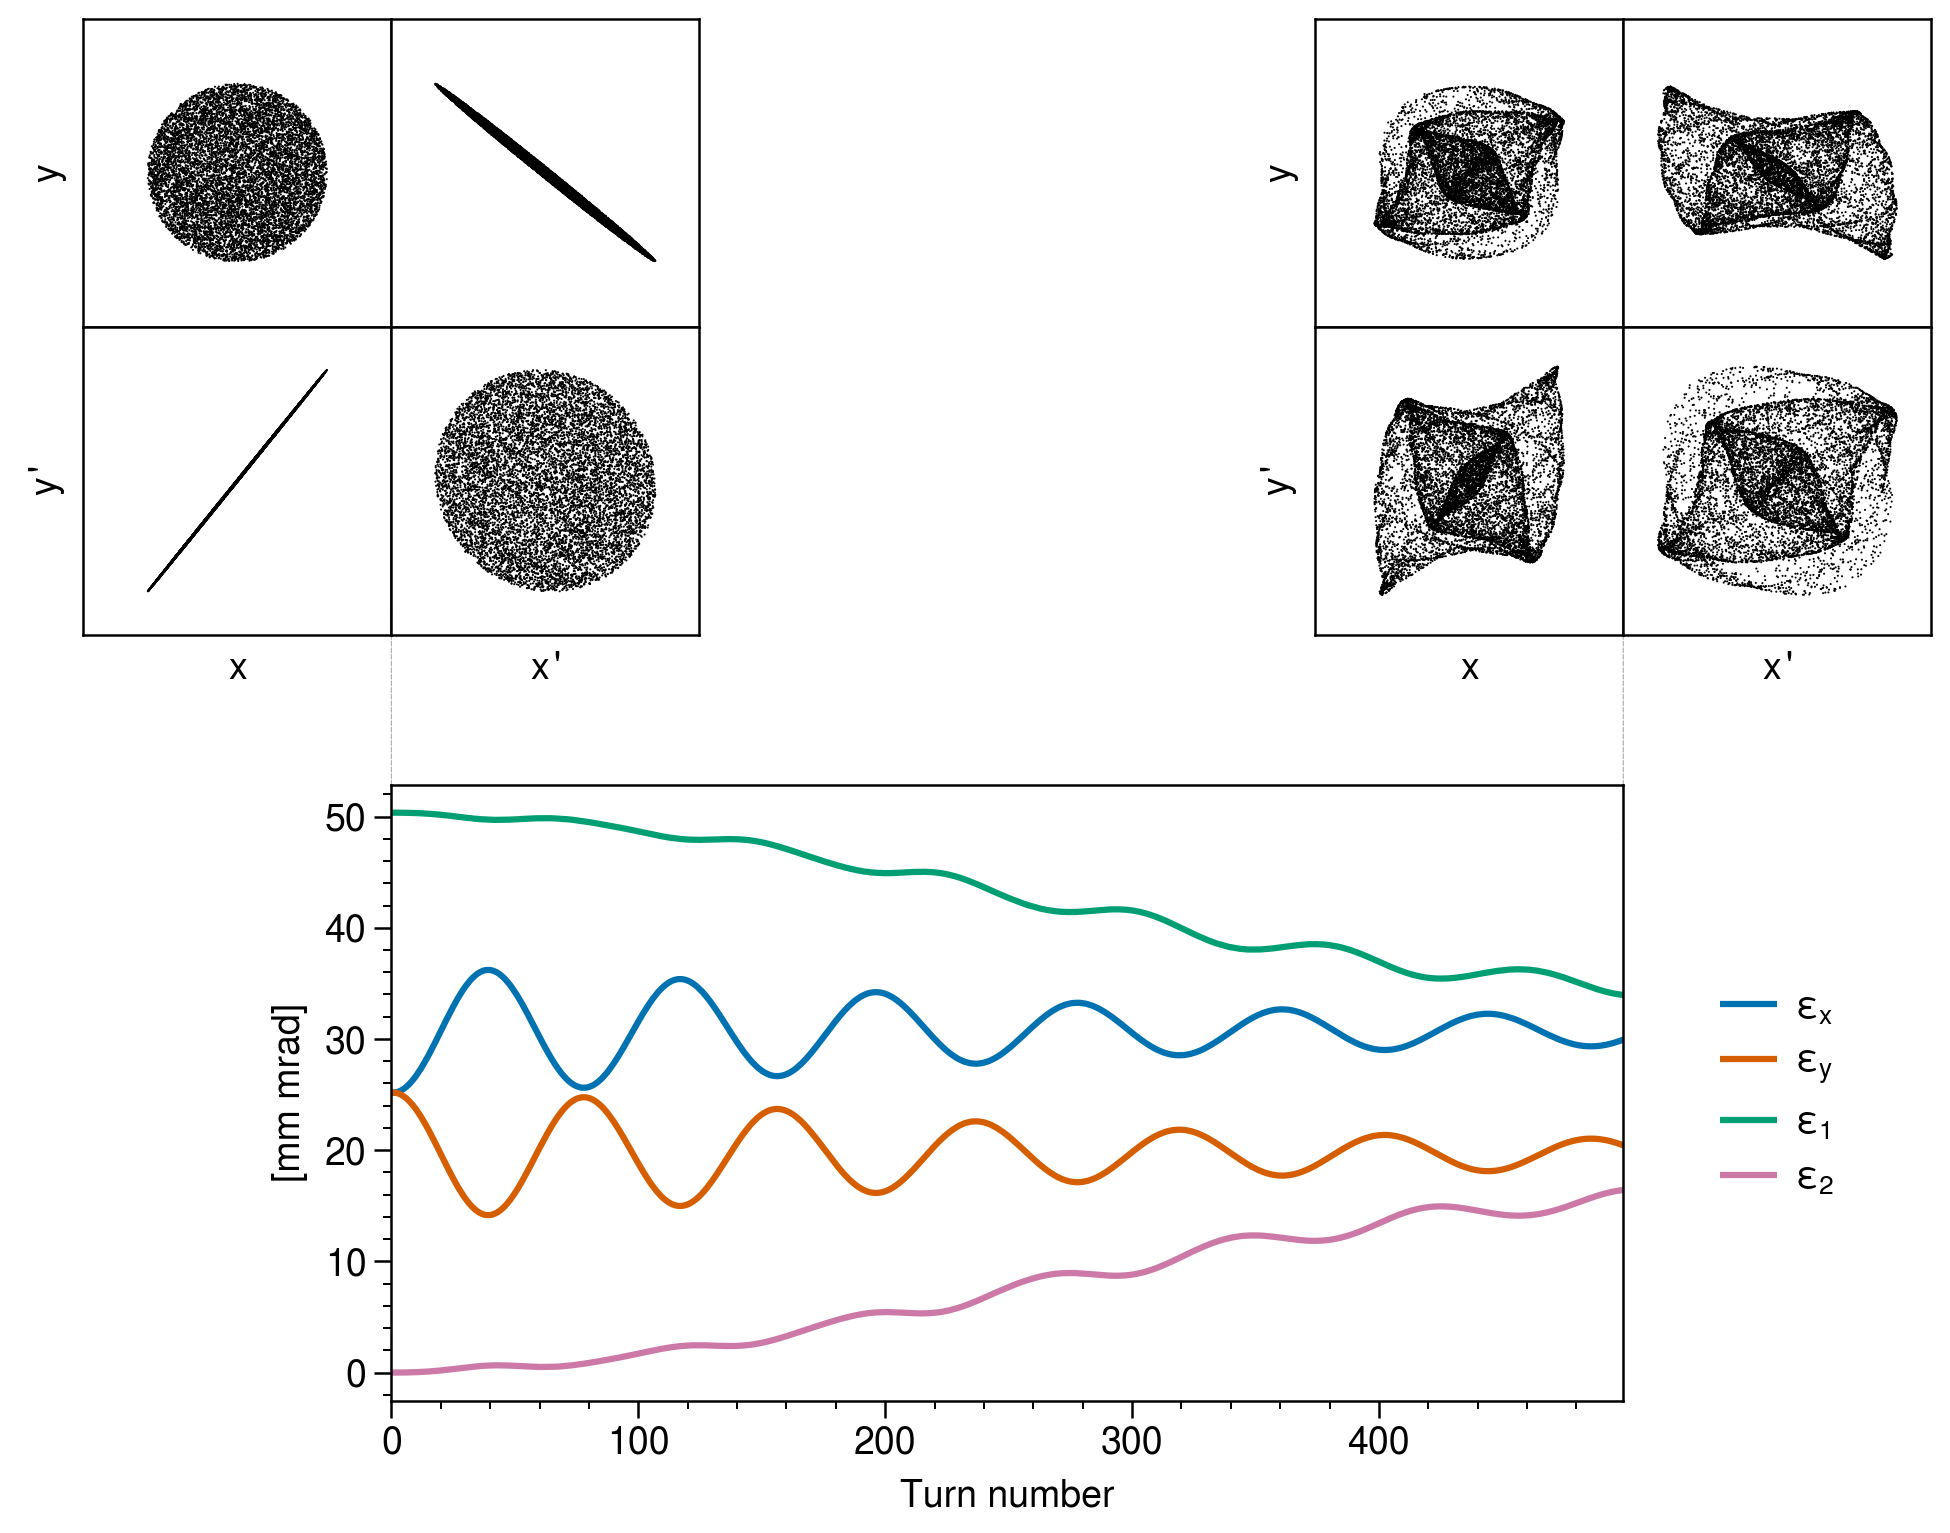
\includegraphics[width=\textwidth]{Images/chapter3/fringe.png}
        \caption{}
        \label{fig:fringe_a}
    \end{subfigure}
    \vfill
    \vspace*{1.5cm}
    \vfill
    \begin{subfigure}{0.7\textwidth}
        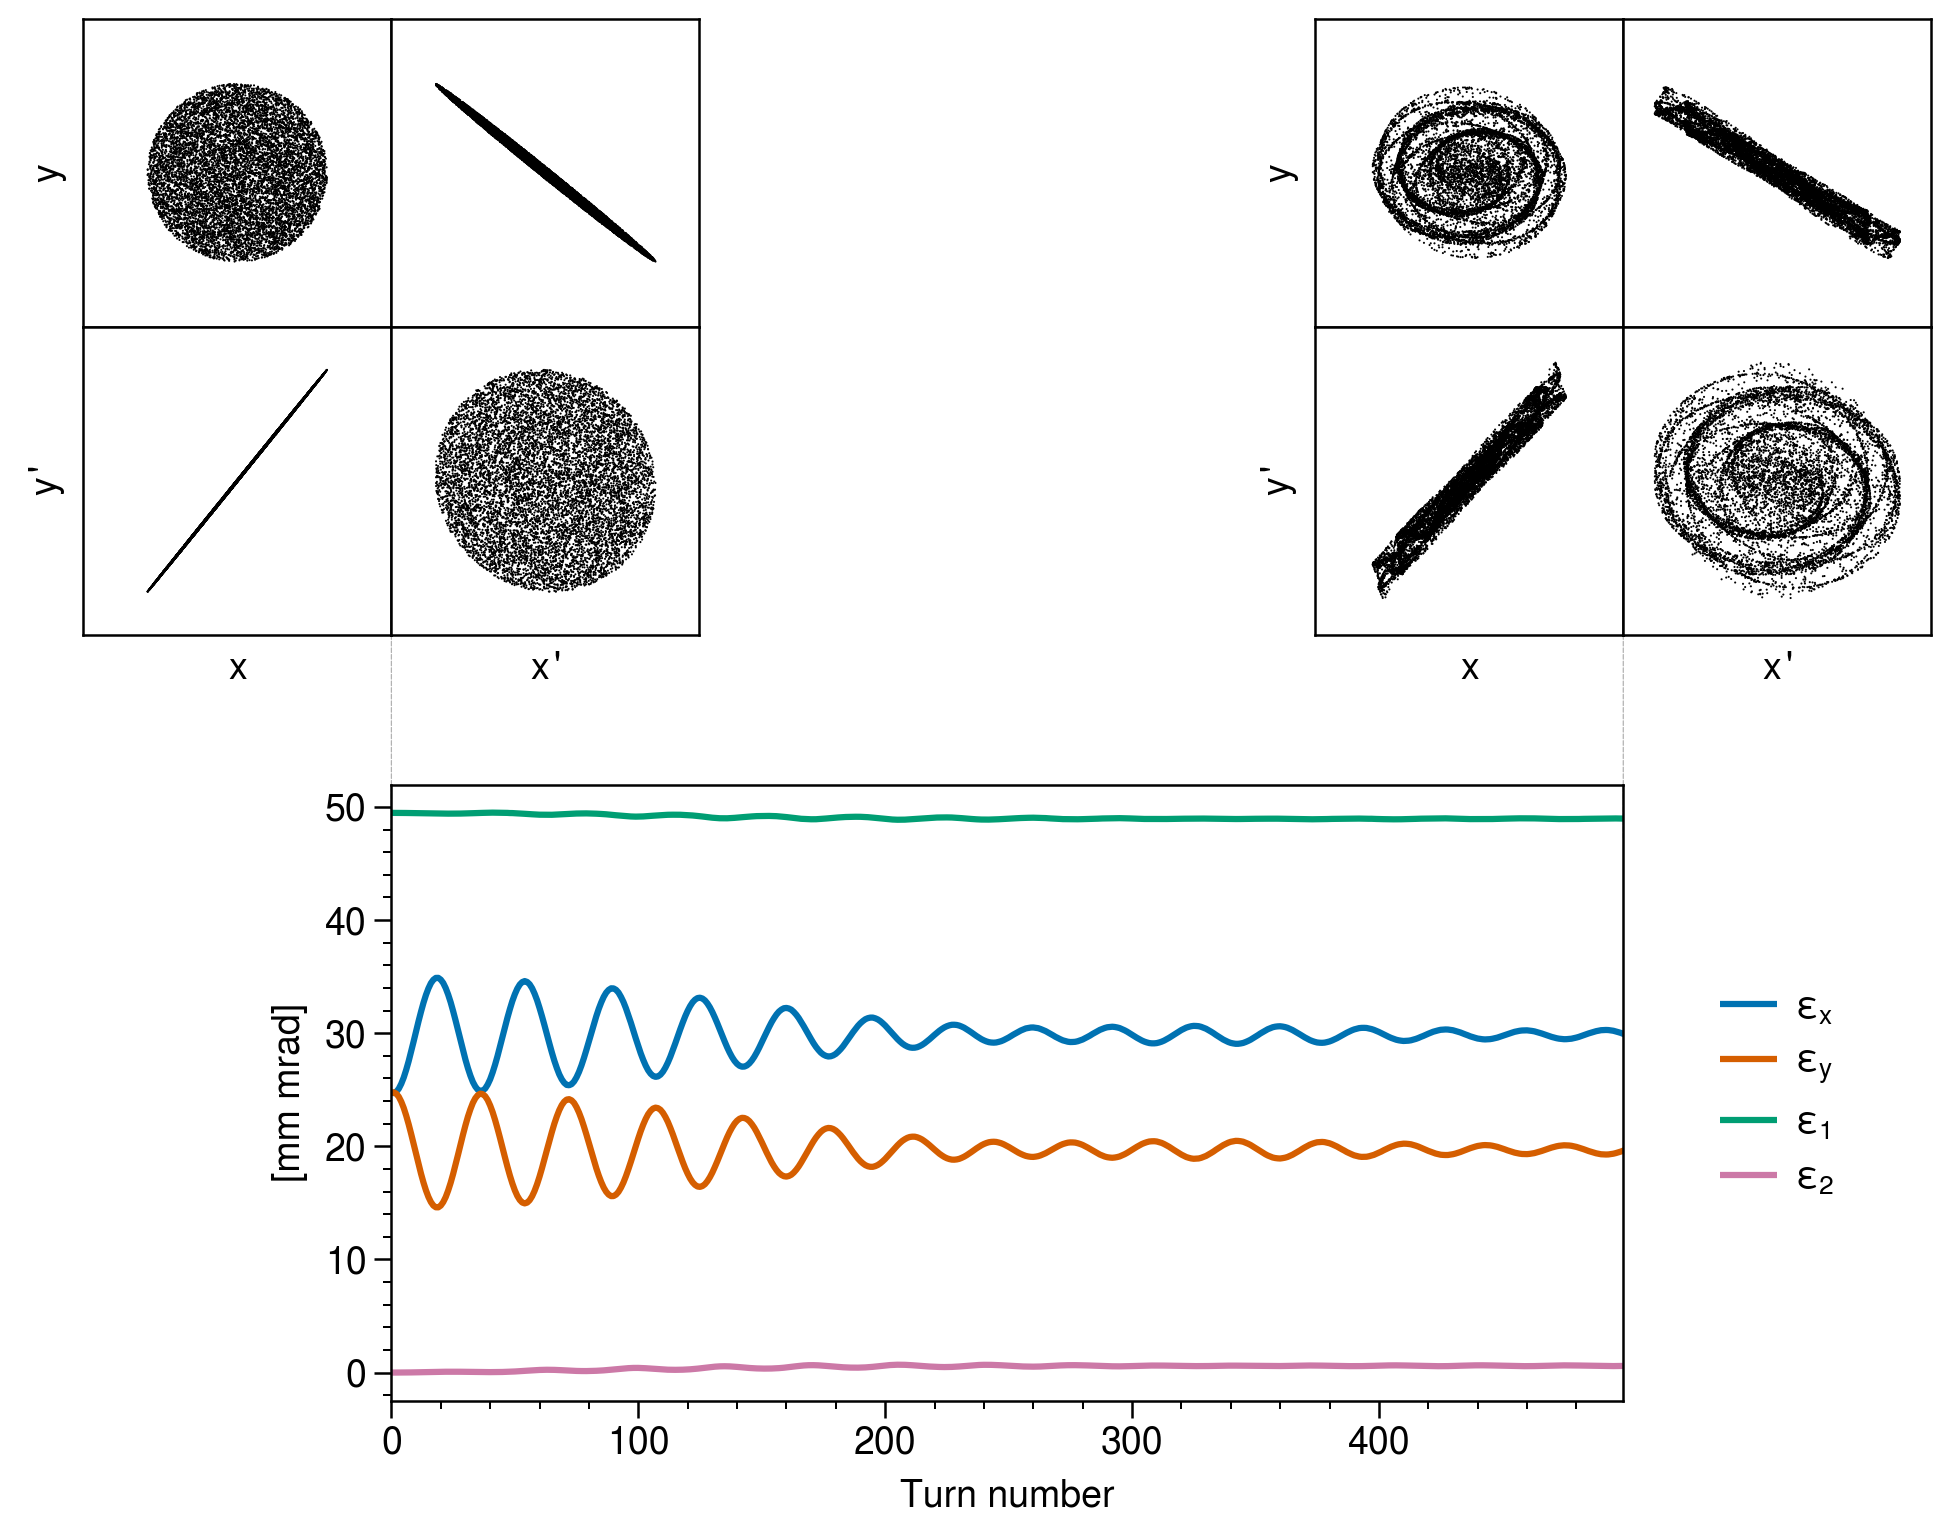
\includegraphics[width=\textwidth]{Images/chapter3/fringe_solenoid.png}
        \caption{}
    \end{subfigure}
    \caption{Danilov distribution tracked in the SNS ring without (a) and with (b) solenoids added to the ring. Fringe fields are the only nonlinear effect included.}
    \label{fig:fringe_b}
\end{figure}
%
In Fig.~\ref{fig:fringe_a}, there is clearly nonlinear coupling between the horizontal and vertical motion; the final distribution is a superposition of rotating and counter-rotating modes. Although the effect of fringe fields is still noticeable, the cross-plane correlations are mostly maintained. The tunes $\nu_{1, 2}$ are no longer equal due to the linear coupling form the solenoid, so the resonance condition is avoided. In Fig.~\ref{}, the simulation is repeated with the inclusion of space charge instead of the solenoid magnet. [...] 


\section{Painting simulations}

The injection process is simulated by adding particles to the bunch at the foil location on each turn. The minipulse from the linac has an RMS emittance of approximately 0.3 mm~mrad. A so-called JOHO distribution is used:
%
%
The beam Twiss parameters are usually assumed to be matched to the lattice ($\beta_x \approx \beta_y \approx 10$ m/rad, $\alpha_x \approx \alpha_y \approx 0$ rad), but recent measurements indicate that they could be significantly different, particularly the $\alpha$ parameter which determines the beam divergence. To be safe, we use values close to these measurements. A Gaussian distribution is used for the longitudinal distribution with RMS energy spread of a few MeV. Since the minipulse is much smaller than the final accumulated pulse, the exact details of the minipulse distribution are not important.


\begin{figure}[!p]
    \centering
    \begin{subfigure}{\textwidth}
        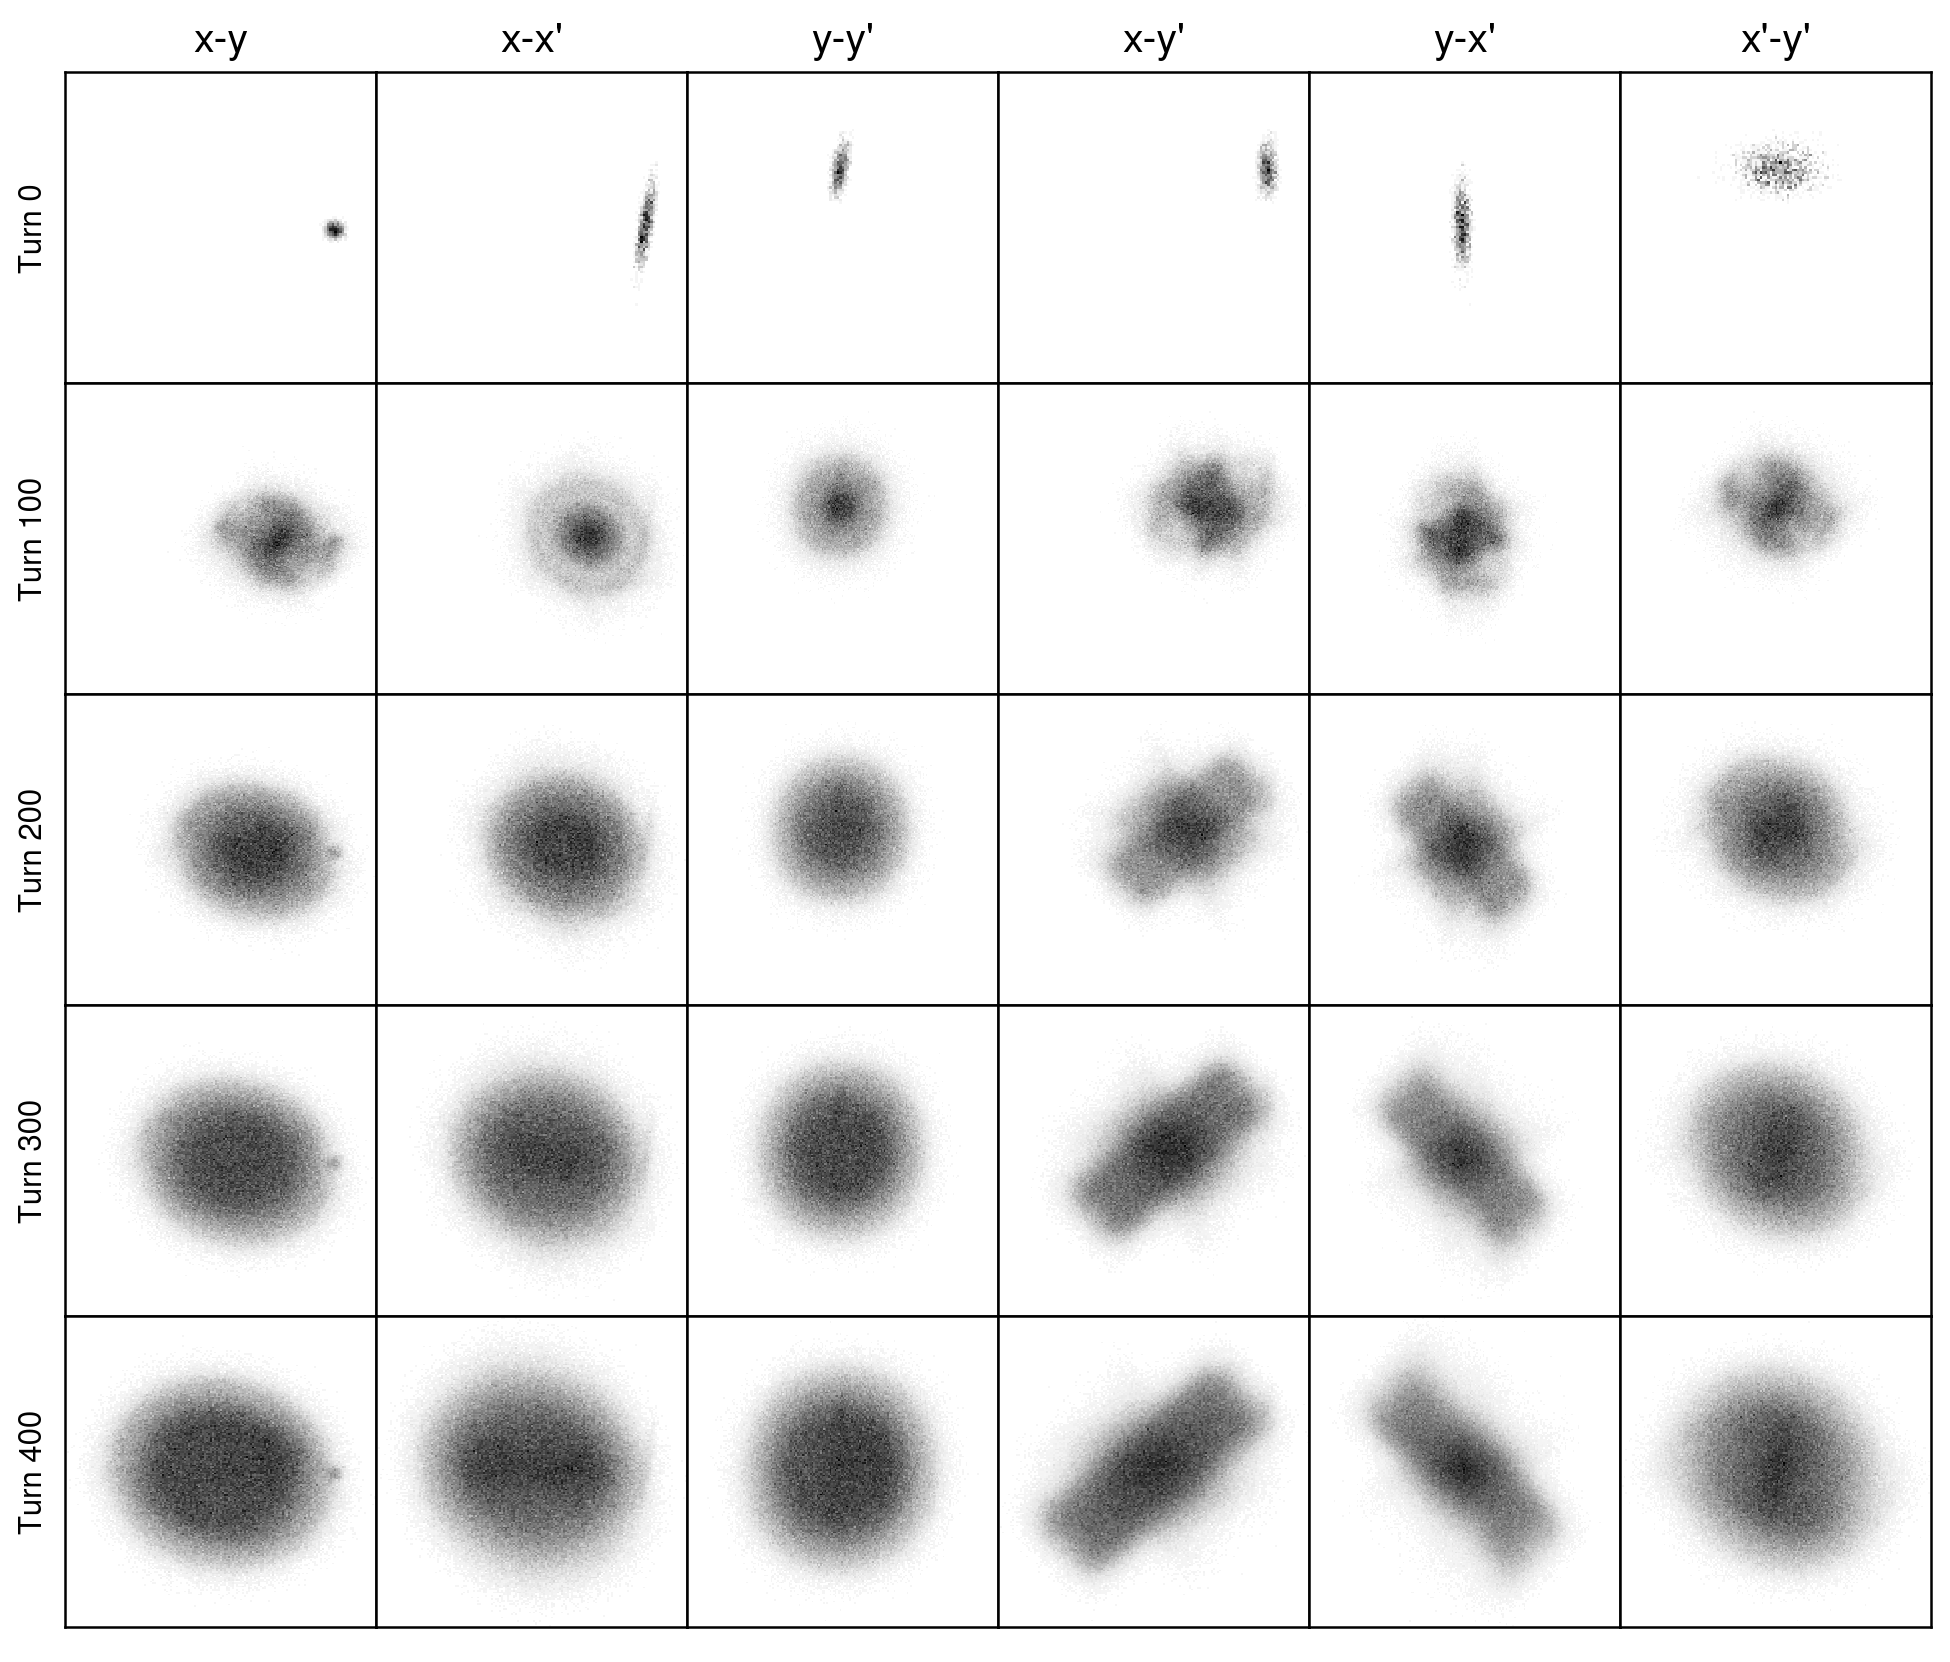
\includegraphics[width=\textwidth]{Images/chapter3/snapshots.png}
    \end{subfigure}
    \vfill
    \vspace*{1.0cm}
    \vfill
    \begin{subfigure}{0.7\textwidth}
        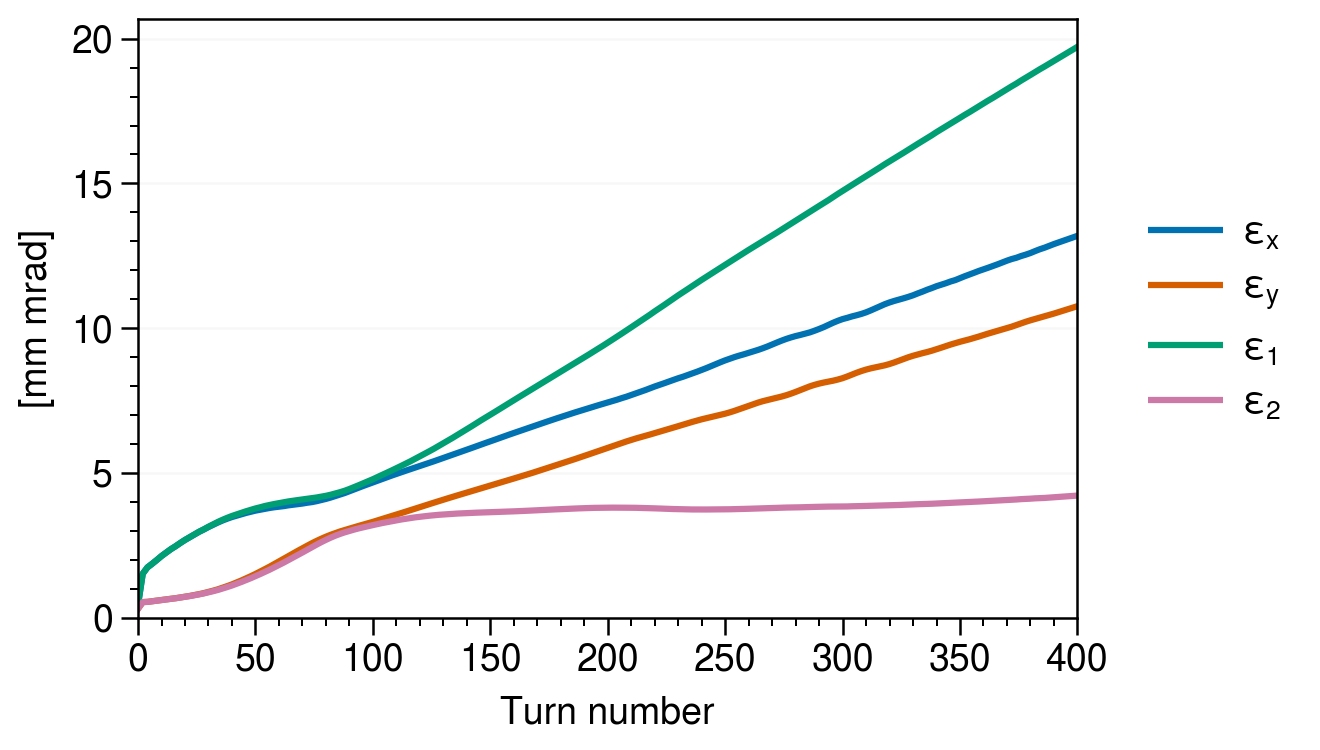
\includegraphics[width=\textwidth]{Images/chapter3/emittances.png}
    \end{subfigure}
    \caption{Simulation of elliptical painting.}
    \label{fig:my_label}
\end{figure}
\chapter{Diagnostics} \label{chap-4}

Determining the similarity between a painted distribution in the SNS and a Danilov distribution requires measurement of the 4D transverse phase space distribution. A direct measurement using a slit-scan \cite{Cathey2018} is not possible at high energy, so the distribution must be reconstructed from lower-dimensional projections. In this chapter, we first detail the available hardware and constraints in the SNS. We then describe methods to perform the reconstruction using 1D and 2D projections. These methods are simulated, then implemented in the SNS.


\section{Available hardware and constraints}

The phase space measurement must be performed in the ring-target beam transfer (RTBT) section of the SNS after the beam has been accumulated in the ring. The RTBT is effectively an extension of the ring that is traversed only once. It is straightforward to vary the number of accumulated turns to measure the beam at any time during injection. 

The RTBT optics are shown in Fig.~\ref{fig:rtbt_optics} along with the locations of four wire-scanners near the target.
%
\begin{figure}[!p]
    \includegraphics[width=\textwidth]{Images/chapter4/RTBT_optics4.png}
    \caption{$\beta$ functions and phase advances in the RTBT wire-scanner region.}
    \label{fig:rtbt_optics}
\end{figure}
%
The wire-scanners measure 1D projections of the distribution by sweeping a wire across the beam path. Each wire-scanner — WS20, WS21, WS23, and WS24 — is equipped with a horizontal, vertical, and diagonal wire. The $\langle{xx}\rangle$, $\langle{yy}\rangle$, and $\langle{uu}\rangle$ moments can be estimated from these projections, where the $u$ axis corresponding to the diagonal wire is tilted at angle $\phi = \pi/4$ above the $x$ axis. From these moments, $\langle{xy}\rangle$ is calculated:
%
\begin{equation}
    \langle{xy}\rangle = \frac{\langle{uu}\rangle - \langle{xx}\rangle \cos^2\phi - \langle{yy}\rangle \sin^2\phi}{2\sin\phi\cos\phi}
    .
\end{equation}
%
The four wire-scanners can be run in parallel and take approximately five minutes to move across the beam and return to their original positions. Their default resolution is around 1 mm and their dynamic range is approximately 100. They are run at a beam pulse frequency of 1 Hz, with each data point corresponding to a separate beam pulse. 

The SNS employs a target imaging system (TIS) to measure the 2D projection of the distribution on the target \cite{Blokland2010}. The SNS target is a stainless steel vessel containing liquid mercury. Its nose is prepared with a Cr:Al2O3 coating that releases light when impacted by the proton beam. Due to the high-radiation environment, the light is collected by a mirror, deflected, and focused onto an optical fiber bundle which guides the light to a camera some distance away. The TIS configuration is shown in Fig.~\ref{fig:tis}.
%
\begin{figure}[!p]
    \centering
    \begin{subfigure}{\textwidth}
        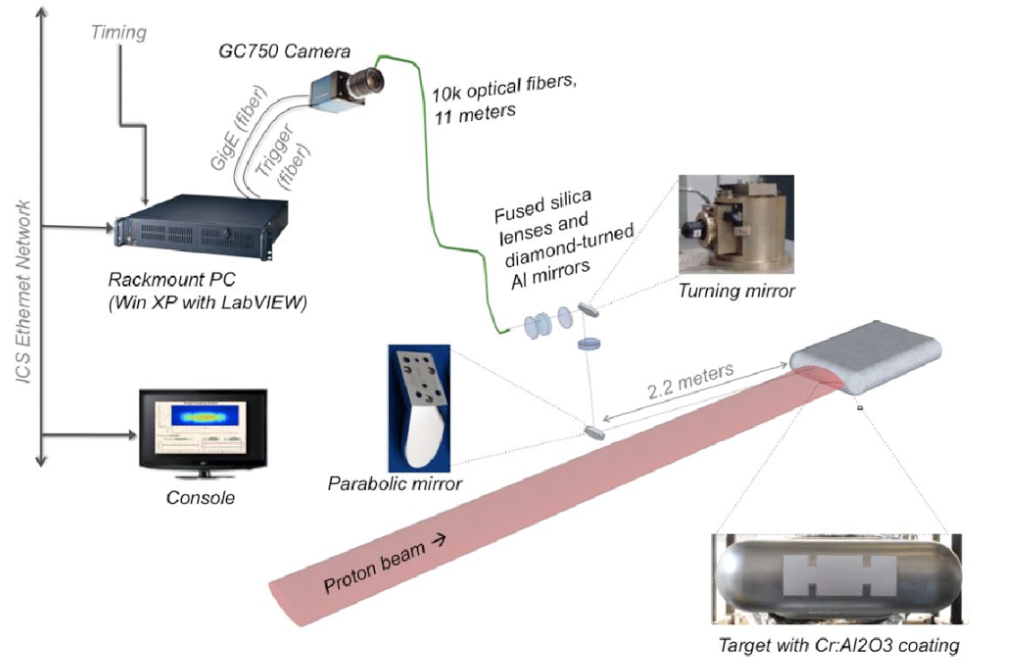
\includegraphics[width=\textwidth]{Images/chapter4/tis1.png}
        \caption{}
        \label{fig:tis_a}
    \end{subfigure}
    \vfill
    \vspace*{2.0cm}
    \vfill
    \begin{subfigure}{0.5\textwidth}
        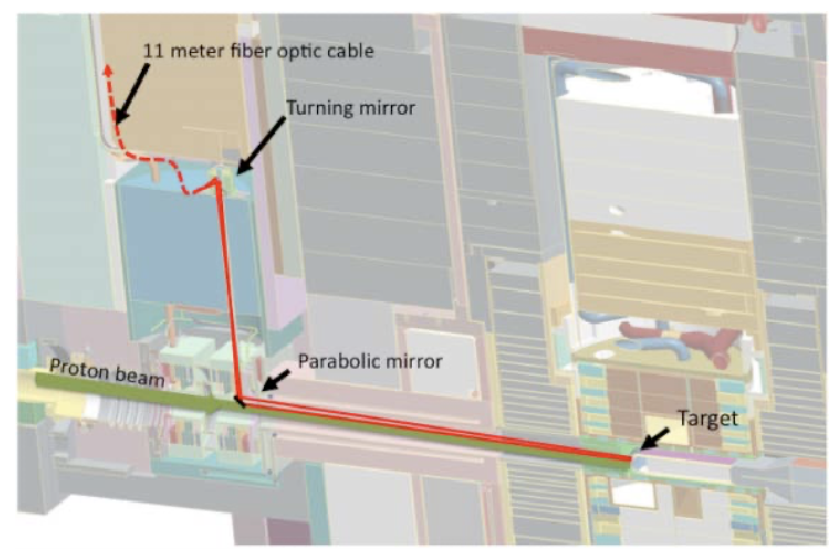
\includegraphics[width=\textwidth]{Images/chapter4/tis2.png}
        \caption{}
        \label{fig:tis_b}
    \end{subfigure}
    \caption{(a) Configuration of the SNS target imaging system. (b) View of the optical path with shielding. (From \cite{Blokland2010}.)}
    \label{fig:tis}
\end{figure}
%

The optics in the RTBT region can be modified, but there are constraints. The $\beta$ functions should be kept below $\approx$ 35 m/rad in the wire-scanner region and below $\approx$ 100 m/rad closer to the target to avoid excess beam loss. At the target, it is best to keep the $\beta$ functions near their default values of $\beta_x \approx$ 60 m/rad and $\beta_y \approx$ 6 m/rad to satisfy peak density requirements on the target. In addition to these constraints, quadrupoles in the wire-scanner region share power supplies. There is a horizontal group \{QH18, QH20, QH22, QH24\} and a vertical group \{QV19, QV21, QV23, QV25\}. The last five magnets — QH26, QV27, QH28, QV29, and QH30 — are individually controlled.


\section{Phase space reconstruction from 1D projections}

\subsection{Method description}

The covariance matrix $\bm{\Sigma}$ can be reconstructed from 1D projections \cite{book:Minty2003, Woodley2000, Prat2014}. We seek to reconstruct $\bm{\Sigma}$ at position $a$ by measuring $\langle{xx}\rangle$, $\langle{yy}\rangle$ and $\langle{xy}\rangle$ at postion $b$, downstream of $A$. Assuming linear transport, the two covariance matrices are related by
%
\begin{equation}
    \bm{\Sigma}_b = \mathbf{M} \bm{\Sigma}_a \mathbf{M}^T,
\end{equation}
%
where $\mathbf{M}$ is the linear transfer matrix from $a$ to $b$. We repeat the measurement at least four times with different transfer matrices — either by changing the measurement location or by changing machine optics — and write
%
\begin{equation}
    \begin{bmatrix}
        {\langle{xx}\rangle}^{(1)} \\
        {\langle{xy}\rangle}^{(1)} \\
        {\langle{yy}\rangle}^{(1)} \\
        {\langle{xx}\rangle}^{(2)} \\
        {\langle{xy}\rangle}^{(2)} \\
        {\langle{yy}\rangle}^{(2)} \\
        {\langle{xx}\rangle}^{(3)} \\
        {\langle{xy}\rangle}^{(3)} \\
        {\langle{yy}\rangle}^{(3)} \\
        \vdots
    \end{bmatrix}_b
    = \mathbf{A}
    \begin{bmatrix}
        \langle{xx}\rangle \\
        \langle{xx'}\rangle \\
        \langle{xy}\rangle \\
        \langle{xy'}\rangle \\
        \langle{x'x'}\rangle \\
        \langle{x'y}\rangle \\
        \langle{x'y'}\rangle \\
        \langle{yy}\rangle \\
        \langle{yy'}\rangle \\
        \langle{y'y'}\rangle \\
    \end{bmatrix}_a
    .
\end{equation}
%
The superscripts represent the measurement index. The coefficient matrix $\mathbf{A}$ for a single measurement is
%
\begin{equation}
    \mathbf{A}^T = 
    \begin{bmatrix}
        M_{11}M_{11} & M_{11}M_{31} & M_{31}M_{31} \\
        2M_{11}M_{12} & M_{12}M_{31} + M_{11}M_{32} & 2M_{31}M_{32} \\
        2M_{11}M_{13} & M_{13}M_{31} + M_{11}M_{33} & 2M_{31}M_{33} \\
        2M_{11}M_{14} & M_{14}M_{31} + M_{11}M_{34} & 2M_{31}M_{34} \\
        M_{12}M_{12} & M_{12}M_{32} & M_{32}M_{32} \\
        2M_{12}M_{13} & M_{13}M_{32} + M_{12}M_{33} & 2M_{32}M_{33} \\
        2M_{12}M_{14} & M_{14}M_{32} + M_{12}M_{34} & 2M_{32}M_{34} \\
        M_{13}M_{13} & M_{13}M_{33} & M_{33}M_{33} \\
        2M_{13}M_{14} & M_{14}M_{33} + M_{13}M_{34} & 2M_{33}M_{34} \\
        M_{14}M_{14} & M_{14}M_{34} & M_{34}M_{34}
    \end{bmatrix}
\end{equation}
%
where $M_{ij}$ is the $i$,$j$ element of the transfer matrix for that measurement. The system is solved using linear least squares (LLSQ). 

The measurement has a geometric interpretation, illustrated in  Fig.~\ref{fig:ws_emittance_measurement} for the 2D case. 
%
\begin{figure}[!p]
    \centering
    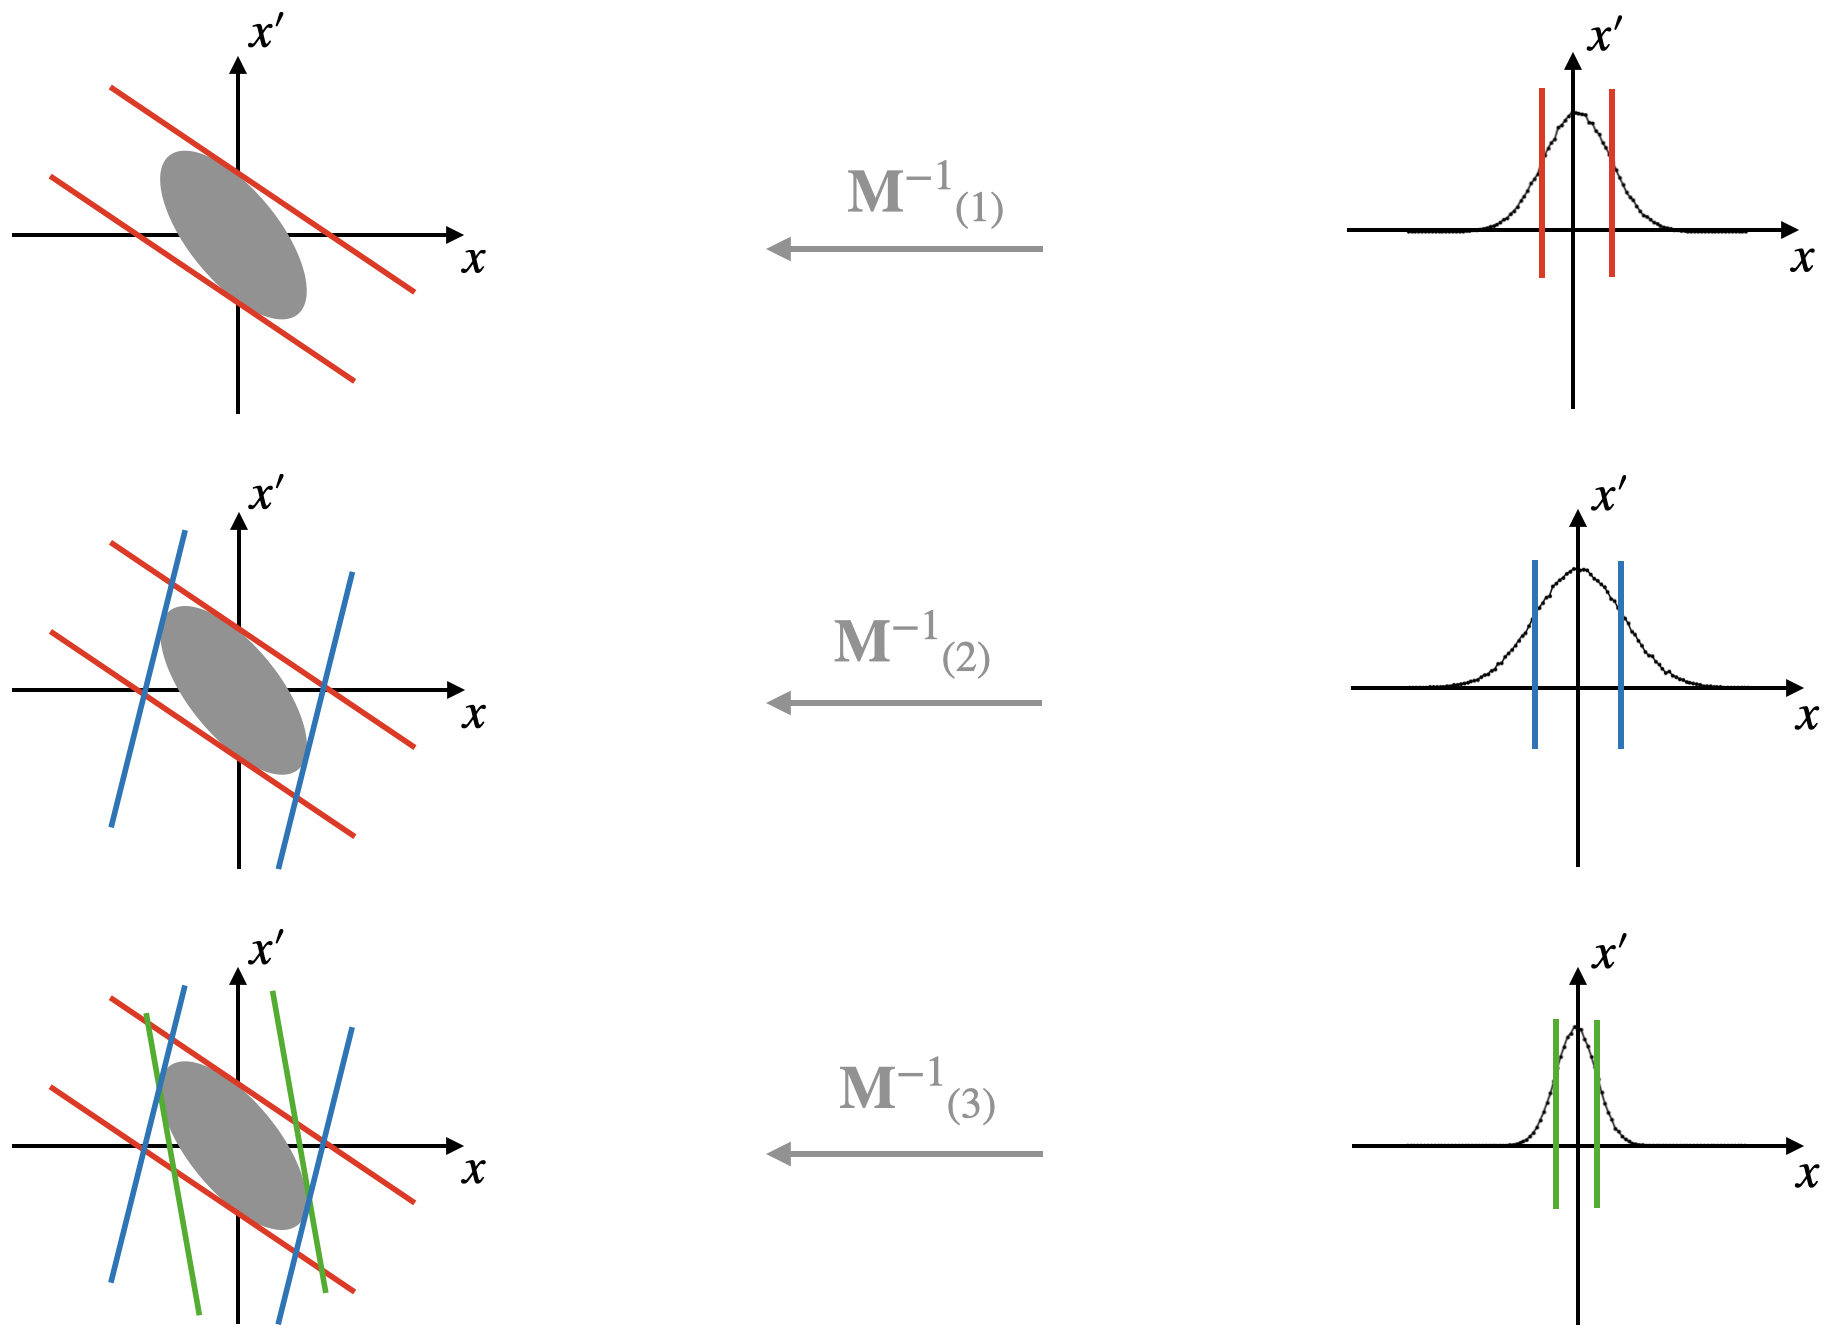
\includegraphics[width=\textwidth]{Images/chapter4/ws_emittance_measurement.png}
    \caption{Illustration of 2D emittance measurement.}
    \label{fig:ws_emittance_measurement}
\end{figure}
%
Each measured beam size defines two lines in the $x$-$x'$ plane at $b$. When the lines are transported back to $a$, their intersection bounds the phase space ellipse. In the general case, each measurement at $b$ defines a 2D surface in 4D phase space (an ellipse in the $x$-$y$ plane with unknown $x'$ and $y'$), and the intersection of these surfaces at $a$ bounds the phase space ellipsoid.


\subsection{Implementation in the SNS}

The four SNS wire-scanners produce four equations, exactly determining the cross-plane moments, so no optics changes are needed in principle; however, additional measurements should reduce the error. In the 2D case, is typically recommended to space $n$ measurements by $\pi / n$ in phase advance \cite{book:Minty2003}. This may be due to the geometric interpretation of Fig.~\ref{fig:ws_emittance_measurement}: in normalized phase space, the rotation angle of the measurement lines is equivalent to the phase advance and the lines are evenly spaced around the phase space ellipse. But in the general case, the angle is given by \cite{Hock2011}
%
\begin{equation}
    \tan\theta = \frac{M_{12}}{M_{11}},
\end{equation}
%
so the spacing will not be uniform. This issue should therefore be investigated numerically in each lattice. The four wire-scanners in the RTBT are already somewhat evenly spaced in phase advance, and it was determined that a 30$\degree$ window around each wire-scanner would provide sufficient coverage. 

Another option, recognized late in this research project, is to compute the RMS moments from the images of the distribution on the target. These images can be collected rapidly, and the $x$-$y$ correlation is computed directly instead of indirectly using a diagonal wire. The use of target images will be explored in the next chapter; the rest of this section focuses only on the wire-scanner measurement.

Due to the shared power supplies of the quadrupoles in the wire-scanner region, there is limited control of the phase advances between the wire-scanners. We instead vary the horizontal and vertical phase advances from QH18 (the first varied quadrupole) to WS24 (the last wire-scanner). This changes the phase advances at WS20, WS21, and WS23 by approximately the same amount. 

To set the phase advances at WS24 while constraining the beam size in the wire-scanner region, the two power supplies (eight quadrupoles) upstream of WS24 were varied using an optimizer that minimizes the following cost function:
%
\begin{equation}
    C(\mathbf{g}) = \left\Vert{\tilde{\bm{\mu}} - \bm{\mu} }\right\Vert^2
    + 
    \epsilon
    \left\Vert
    \Theta\left(
        \tilde{\bm{\beta}}_{max} - \bm{\beta}_{max}
    \right)
    \right\Vert^2
    .
\end{equation}
%
The quadrupole field strengths are contained in the vector $\mathbf{g}$. The calculated and desired phase advances at WS24 are $\bm{\mu} = (\mu_x, \mu_y)$, and $\tilde{\bm{\mu}} = (\tilde{\mu}_x, \tilde{\mu}_y)$, respectively. The maximum calculated and allowed $\beta$ functions in the wire-scanner region are $\bm{\beta} = (\beta_{x_{max}}, \beta_{y_{max}})$ and $\tilde{\bm{\beta}}_{max} = (\tilde{\beta}_{x_{max}}, \tilde{\beta}_{y_{max}})$, respectively. $\Theta$ is the Heaviside step function. Finally, $\epsilon$ is a constant. It is hoped that the beam is matched to the lattice optics so that the calculated phase advances are close to the true phase advances.

A GUI application was developed in the OpenXAL framework for use in the SNS control room. In the first pane of the application, the user can set the phase advances at WS24 and view the model optics and phase advances throughout the RTBT. In the second pane, the user can load wire-scanner output files and choose the reconstruction location. These files are output from a separate application and contain the wire-scanner profiles, RMS parameters, and Gaussian fit parameters. They also contain a number that defines the machine state — magnet strengths, etc. — at the time of the measurement. The application reads this number, synchronizes the model with the machine state, and computes the transfer matrices from the wire-scanners to the reconstruction location. The RMS moments and transfer matrices are then used to reconstruct the covariance matrix. The resulting beam parameters are printed and compared to the model lattice parameters. The 2D projections of the covariance ellipsoid are plotted along with the measurement lines, with the option to view in normalized coordinates. 



\subsection{Measurement of a production beam}

The multi-optics method was tested on a fully accumulated production beam. The phase advances at WS24 were varied in a 30$\degree$ range over ten steps — the first half of the scan held the vertical phase fixed while varying the horizontal phase, and the second half of the scan held the horizontal phase fixed while varying the vertical phase. The results of the reconstruction are shown in Fig.~\ref{fig:prod_meas} for a location just before QH18.
%
\begin{figure}[!p]
    \centering
    \begin{subfigure}{0.8\textwidth}
        \centering
        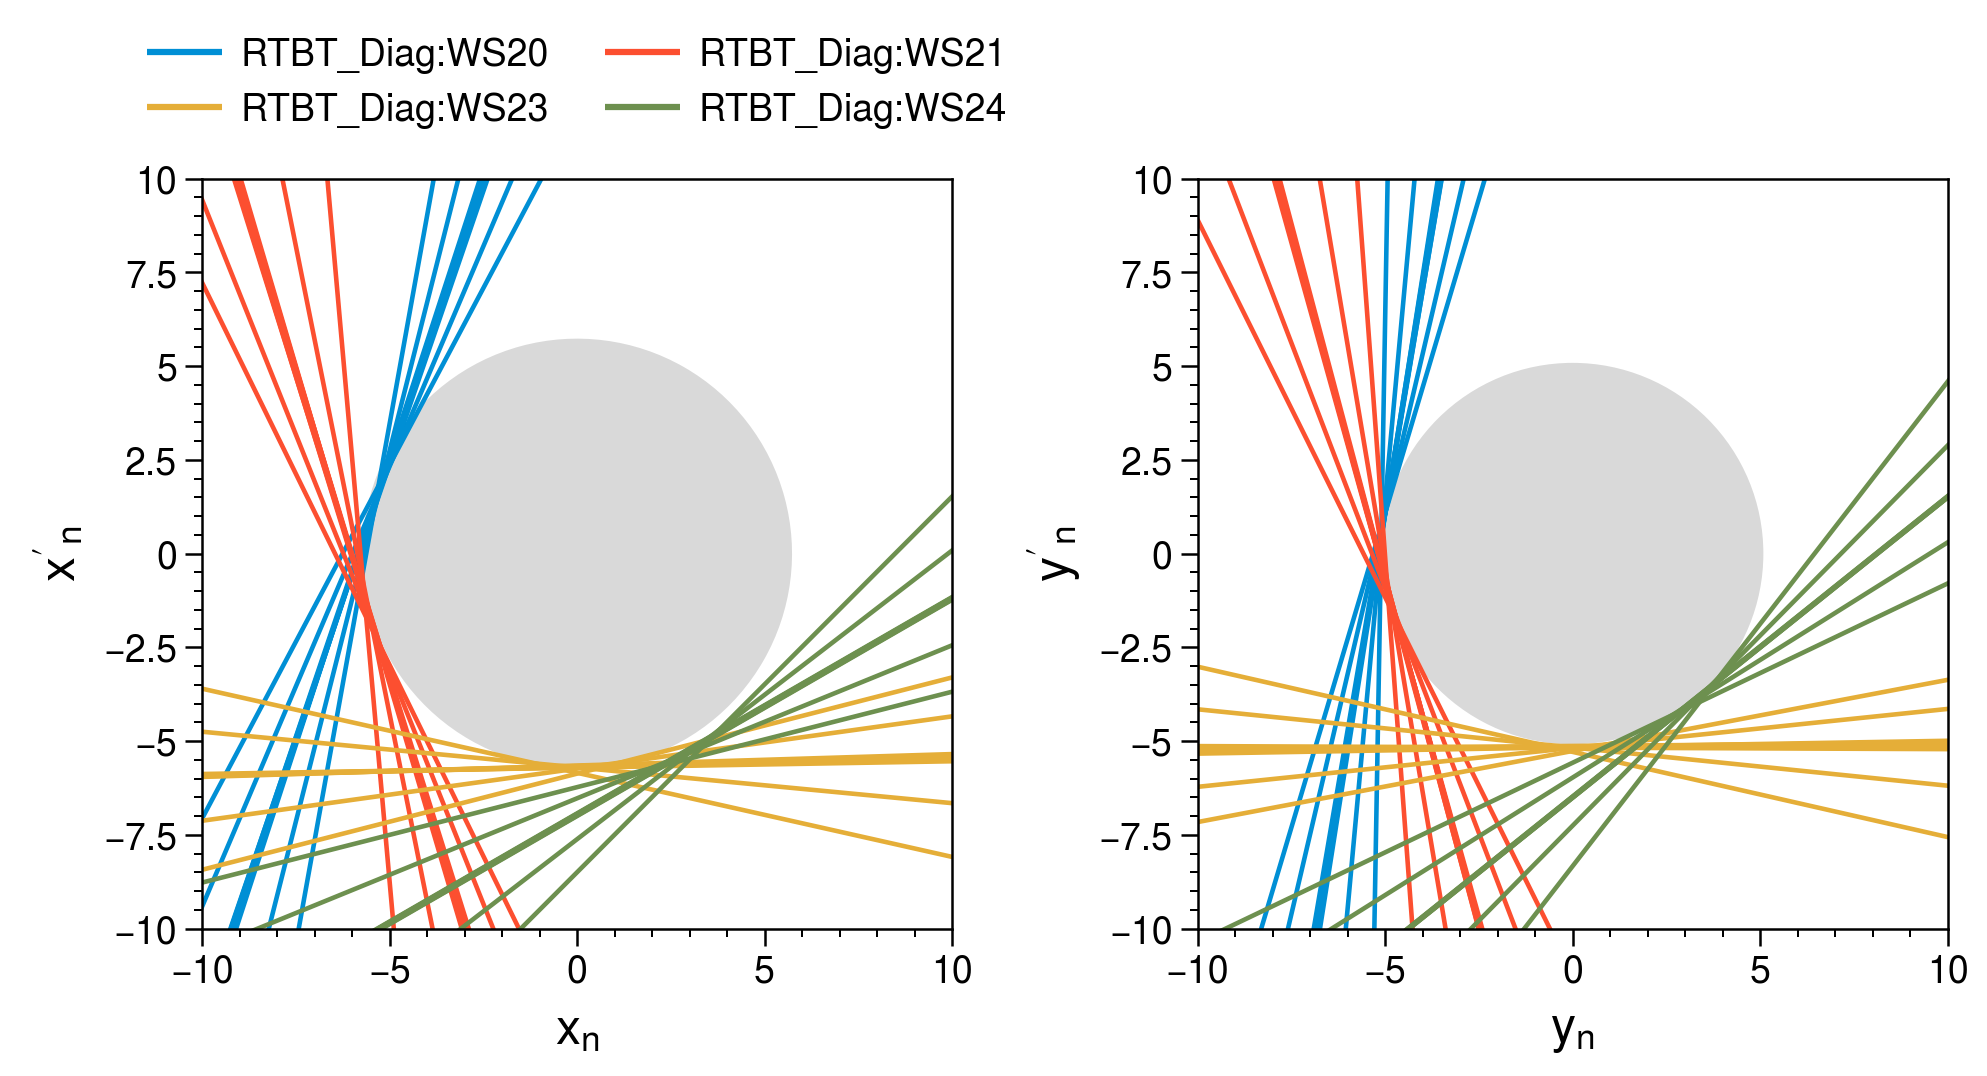
\includegraphics[width=\textwidth]{Images/chapter4/prod_meas_lines.png}  
    \end{subfigure}
    \par\medskip
    \begin{subfigure}{0.6\textwidth}
        \centering
        \begin{tabular}{lcc}
            \small\textbf{Parameter} & \small\textbf{Measurement} & \small\textbf{Model} \\
            \midrule
            \small$\beta_x$ [m/rad] & \small22.06 $\pm$ 0.29 & \small22.00 \\
            \small$\beta_y$ [m/rad] & \small4.01 $\pm$ 0.02 & \small3.81 \\
            \small$\alpha_x$ [rad] & \small2.33 $\pm$ 0.04 & \small2.37 \\
            \small$\alpha_y$ [rad] & \small-0.49 $\pm$ 0.01 & \small-0.60 \\
            \small$\varepsilon_1$ [mm~mrad] & \small33.02 $\pm$ \small0.05 & - \\
            \small$\varepsilon_2$ [mm~mrad] & \small25.67 $\pm$ \small1.03 & - \\
            \small$\varepsilon_x$ [mm~mrad] & \small32.85 $\pm$ \small0.05 & - \\
            \small$\varepsilon_y$ [mm~mrad] & \small25.87 $\pm$ \small0.12 & - \\
          \end{tabular}
    \end{subfigure}
    \par\medskip
    \caption{Reconstructed beam parameters and graphical output from a multi-optics emittance measurement of a production beam.}
    \label{fig:prod_meas}
\end{figure}
%
The best-fit ellipses in the $x$-$x'$ and $y$-$y'$ planes are normalized by the reconstructed Twiss parameters. The uncertainties in the beam parameters were calculated by propagating the standard deviations of the ten reconstructed moments obtained from the LLSQ estimator. The reconstructed Twiss parameters are close to the model parameters computed from the linear transfer matrices of the ring and RTBT, showing that the beam is matched. The intrinsic emittances are almost equal to the apparent emittances, showing that there is very little cross-plane correlation. This is expected for a production beam.

Decreasing the number of measurements used in the reconstruction had no substantial effect on the answer as long as at least two measurements (eight profiles) were used; however, the fit usually failed when only one measurement (four profiles) was used. Here, ``failed fit" means that the reconstructed covariance matrix is unphysical, producing imaginary intrinsic emittances. 



\subsection{Sensitivity to measurement errors}

A nonlinear solver can be used to ensure that the reconstructed covariance matrix is physical; however, the answer was found to depend strongly on the initial guess provided to the solver. To investigate the failure of the fixed-optics method, the reconstructed covariance matrix (using the full data set) was tracked to the wire-scanners using the known transfer matrices. Random Gaussian noise was added to the moments at these locations, and the noisy moments were used to perform the reconstruction. This was repeated for several trials. It was found that the reconstruction was extremely sensitive to changes in the beam moments, as shown in Fig.~\ref{fig:prod_sensitivity}.
%
\begin{figure}[!p]
    \centering
    \begin{subfigure}{1.0\textwidth}
        \includegraphics[width=\textwidth]{Images/chapter4/prod_sensitivity1.png}
    \end{subfigure}
    \vfill
    \vspace*{0.5cm}
    \vfill
    \begin{subfigure}{1.0\textwidth}
        \includegraphics[width=\textwidth]{Images/chapter4/prod_sensitivity2.png}
    \end{subfigure}
    \vfill
    \vspace*{0.5cm}
    \vfill
    \begin{subfigure}{1.0\textwidth}
        \includegraphics[width=\textwidth]{Images/chapter4/prod_sensitivity3.png}
    \end{subfigure}
    \caption{Monte Carlo trials of a fixed-optics emittance measurement in the RTBT. Left: apparent emittances.}
    \label{fig:prod_sensitivity}
\end{figure}
%
As soon as any noise is included, the fail rate jumps to a large value; additionally, the intrinsic emittances reconstructed in the successful fits have a large, asymmetric spread around the correct values. On the other hand, the apparent emittances are localized around the correct values. (The transfer matrices are uncoupled, so the $x$-$x'$ and $y$-$y'$ reconstructions are performed independently. The problem is with the cross-plane moments.)

Sensitivity of 4D emittance measurements using fixed-optics was observed in \cite{Woodley2000}, including the asymmetric distribution of errors in Fig.~\ref{fig:prod_meas}. The problem was studied more recently in \cite{Agapov2007} and \cite{Faus-Golfe2016}. The conclusion from these studies is that the linear system for the cross-plane moments is ill-conditioned. The sensitivity of a linear system $\mathbf{A} \mathbf{x} = \mathbf{b}$ to errors in $\mathbf{b}$ is determined by the condition number of $\mathbf{A}$, which is the product of matrix norms $\Vert \mathbf{A} \Vert \Vert \mathbf{A}^{-1} \Vert$. As an example, consider four wire-scanners that are evenly spaced in phase advance and connected by rotation matrices. Fig.~\ref{fig:fodo_condition_number} plots the condition number of the coefficient matrix as a function of the spacing between the wire-scanners.
%
\begin{figure}[!p]
    \centering
    \includegraphics[width=0.7\textwidth]{Images/chapter4/fodo_condition_number.png}
    \caption{Condition number $C$ of the coefficient matrix for four wire-scanners that are evenly spaced in phase advance and connected by rotation matrices.}
    \label{fig:fodo_condition_number}
\end{figure}
%
The condition number is large when the spacing is 90\degree, in which case the two measurements provide degenerate information in $x$-$x'$ or $y$-$y'$. The sum and difference lines correspond to the cross-plane moments. The chart will be more complicated for different optics or additional wire-scanners.

Fig.~\ref{fig:rtbt_condition_number} shows a similar calculation in the RTBT. 
%
\begin{figure}[!p]
    \centering
    \begin{subfigure}{0.75\textwidth}
        \includegraphics[width=1.0\textwidth]{Images/chapter4/rtbt_condition_number.png}
    \end{subfigure}
    \vfill
    \vspace*{0.8cm}
    \begin{subfigure}{0.75\textwidth}
        \includegraphics[width=1.0\textwidth]{Images/chapter4/rtbt_fail_rate.png}
    \end{subfigure}
    \caption{4D emittance reconstruction errors as a function of the phase advances at WS24. Top: condition number of the linear system. Bottom: simulated reconstruction fail rate with 3\% beam size error.}
    \label{fig:rtbt_condition_number}
\end{figure}
%
The phase advances at WS24 are scanned around their default values. The default optics are ill-suited for the measurement. A new operating point was chosen at the blue dot in the figure. This corrected the issue of failed fits in the following experiments. 
% [Unfortunately, the sensitivity of the successful fits to errors — i.e., the variance of the reconstructed emittances — was not examined in detail. We will return to this point in chapter \ref{chap-5}].

Finally, we mention that there is information to be gained from 1D projections of the distribution in addition to the RMS reconstruction. The distributions can be compared to the ideal ``half-circle" projections of a uniform density ellipse. The horizontal and vertical projections can be used to reconstruct the $x$-$x'$ or $y$-$y'$ distribution using the tomographic methods described in the next section. It may be possible to include cross-plane information in the reconstruction using the diagonal projections. There is a particular method that can, in principle, reconstruct the $x$-$x'$-$y$-$y'$ distribution from only 1D projections, although the method is untested. 

[To be added somewhere: simulation of the reconstruction in the RTBT, including all errors. Also simulate a wire-scanner profile and show the expected error in the RMS moments when noise is included.]








\section{Phase space reconstruction from 2D projections}

Tomographic methods are well-established for the reconstruction of 2D phase space distributions from 1D projections in transverse phase space \cite{Hock2014} and longitudinal phase space \cite{Evans2014}. The concept has recently been extended to the reconstruction of the 4D transverse phase space, both in theory and in practice \cite{Hock2013b, Wang2019, Wolski2020}. This section begins with a brief discussion of tomography in two dimensions as applied to particle accelerators, then moves on to describe several 4D reconstruction algorithms — the algorithms are implemented and their accuracy and limitations are discussed. Finally, the use of 4D tomography on images from the SNS target imaging system is discussed.


\subsection{Beam tomography}

Many algorithms exist to reconstruct 2D images from 1D projections, such as filtered back-projection (FBP), algebraic reconstruction (ART) \cite{Slaney1988}, and maximum entropy (MENT) \cite{Minerbo1979}. Projections of an object are normally obtained by illuminating the object at different angles. Although the measured 1D projections of a 2D phase space distribution are always along one direction (the $x$ of $y$ axis), we can take advantage of the known transfer matrix $\mathbf{M}$ between the measurement location $b$ and the reconstruction location $a$. The measured projection at $b$ is
%
\begin{equation}
    p_b(x_b) = \int_{-\infty}^{\infty} f(x_b, x'_b) dx'_b.
\end{equation}
%
Let $\tilde{x}$ be the projection axis $x_b$ transported to $a$. $\tilde{x}_a$ is rotated by an angle $\theta$ relative to $x_a$ \cite{Hock2013a}: 
%
\begin{equation}\label{eq:proj_trans_1}
    \tan\theta = \frac{M_{12}}{M_{11}}.
\end{equation}
%
The distance along the axis will be scaled:
%
\begin{equation}\label{eq:proj_trans_2}
    r = \frac{x_b}{\tilde{x}_a} = \sqrt{M_{11}^2 + M_{12}^2}.
\end{equation}
%
The projections are related by
%
\begin{equation}\label{eq:proj_trans_3}
    p_a(\tilde{x}_a) = r p_b(r\tilde{x}_a).
\end{equation}
%
Standard tomography algorithms can be applied to the transformed projections.

It is also possible to reconstruct in normalized phase space \cite{Hock2011}. Recall the normalization matrix $\mathbf{V}$ from Eq.~\eqref{eq:CS_parameterization}. In normalized coordinates, the transfer matrix is a rotation matrix by an angle equal to the phase advance. It is straightforward to obtain the projections in the normalized phase space at $a$:
%
\begin{equation}
\begin{aligned}
    \mathbf{x} &\rightarrow \mathbf{M} \mathbf{x}
    = \mathbf{M} \mathbf{V} (\mathbf{V}^{-1} \mathbf{x})
    ,
\end{aligned}
\end{equation}
%
where $\mathbf{V}$ is a function of the Twiss parameters at $a$. The previous equations can be applied to the new matrix $\mathbf{M} \mathbf{V}$ to obtain the projections in the normalized phase space at $a$. After the image is reconstructed, the true distribution can be obtained by transforming the grid coordinates using $\mathbf{V}$ and interpolating at the transformed coordinates. Note that any Twiss parameters can be used to form $\mathbf{V}$; if the Twiss parameters are matched to the distribution, the rotation angle of the projection will be the phase advance from $a$ to $b$, and the reconstructed distribution will be circular in the normalized phase space. 



\subsection{4D reconstruction as a series of 2D reconstructions}

Recent work by Hock et al. reduces 4D reconstruction to a series of 2D reconstructions when the $x$-$y$ projections are available \cite{Hock2013a}. The method, which we refer to as Hock's method, is as follows. Assume that the horizontal and vertical angles (or phase advances) can be controlled independently. Let the angles in $x$-$x'$ be \{$\theta_{x_1}$, $\dots$, $\theta_{x_k}$, $\dots, \theta_{x_K}$\} and the angles in $y$-$y'$ be \{$\theta_{y_1}$, $\dots$, $\theta_{y_l}$, $\dots$, $\theta_{y_L}$\}. The projections are stored in an array $\mathbf{S}$, where $\mathbf{S}_{i,j,k,l}$ is the intensity at point ($x_i$, $y_j$) on the screen for angles $\theta_x = \theta_{x_k}$, $\theta_y = \theta_{y_l}$. We can immediately reconstruct a 3D projection of the distribution from this data. Consider a single row of the image — the intensity along the row gives a 1D projection onto the $x$ axis for a horizontal slice of the distribution. We have a set of these 1D projections at different $\theta_{x}$ which we can use to reconstruct the $x$-$x'$ distribution at this slice using any 1D $\rightarrow$ 2D reconstruction method. Repeating at each slice gives the array $\mathbf{D}$, where $\mathbf{D}_{j, l, r, s}$ is the density at $x = x_r$, $x' = x'_s$, $y = y_j$, for $\theta_{y} = \theta_{y_l}$. We then analyze the vertical plane. At each bin in the reconstructed $x$-$x'$ grid, we have a set of 1D projections of $y$-$y'$ at each $\theta_{y_l}$, thus, $y$-$y'$ can be reconstructed. This completes the reconstruction — we have an array $\mathbf{Z}$, where $\mathbf{Z}_{r, s, t, u}$ is the density at $x = x_r$, $x' = x_s$, $y = y_t$, $y' = y'_u$.

To test the method, the 600,000-particle distribution from Fig.~\ref{fig:Holmes_corner_compare} was used. Simultaneous algebraic reconstruction (SART) was used for the 2D reconstructions. The accuracy of SART will depend on the number of projections and the range of projection angles. Fig.~\ref{fig:tomo_sim_art2D} demonstrates this by reconstructing the $x$-$x'$ distribution from 1D projections as these numbers are varied.
%
\begin{figure}[!p]
    \centering
    \includegraphics[width=0.6\textwidth]{Images/chapter4/tomo_sim_art2d.png}
    \caption{Test of SART accuracy as a function of number of projections and range of projection angles.}
    \label{fig:tomo_sim_art2D}
\end{figure}
%
It appears that if the projection angles are distributed over a significant range, the accuracy does not improve much beyond 10-15 projections. As discussed later, 15 projections is likely near the maximum possible in the SNS. Thus, for the 4D reconstruction, the phase advances in both planes were scanned over $180\degree$ in 15 steps; at each step, the distribution was transported to and then binned on a virtual screen. The reconstruction was performed in normalized phase space using the following Twiss parameters: $(\alpha_x, \alpha_y, \beta_x, \beta_y) = (
-0.030,\, 0.213,\, 17.027,\, 9.631)$, which are close, but not equal, to the statistical beam parameters: $\alpha_x, \alpha_y, \beta_x, \beta_y = (0.003,\, 0.125,\, 22.70,\, 11.88)$. Fig.~\ref{fig:tomo_sim_target_scan} shows several of the simulated images in normalized space as the horizontal phase advance is scanned. The screen resolution in the figure is $75 \times 75$.
%
\begin{figure}[!p]
    \centering
    \includegraphics[width=\textwidth]{Images/chapter4/tomo_sim_target_scan.png}
    \caption{Simulated $x$-$y$ projections as the horizontal phase advance is varied.}
    \label{fig:tomo_sim_target_scan}
\end{figure}
%
Hock's method was then applied to these projections. The 2D projections of the reconstructed distribution are compared to the original distribution in Fig.~\ref{fig:tomo_sim_rec_hock_proj_2D}.
%
\begin{figure}[!p]
    \centering
    \includegraphics[width=0.8\textwidth]{Images/chapter4/tomo_sim_rec_hock_proj_2D.png}
    \caption{Simulated reconstruction using Hock's method (normalized phase space).}
    \label{fig:tomo_sim_rec_hock_proj_2D}
\end{figure}
%
The main features of the original distribution are present in the reconstruction.

Hock's method has not yet been experimentally demonstrated, likely due to the long measurement time, but the method is preferred because it leverages 2D reconstruction algorithms. Open-source implementations of these algorithms are widely available and the conditions needed for accurate reconstructions are well-understood, primarily due to the use of tomography in medical imaging. 


\subsection{Direct 4D reconstruction}

If the phase advances cannot be independently controlled or if only a very small number of projections can be collected, 2D reconstruction algorithms must be generalized to 4D. Several algorithms generalize to any number of dimensions, but they may be difficult to implement, the conditions for an accurate reconstruction may be unclear, and the time and space complexity may make the method infeasible. We focus on two methods that have recently been experimentally demonstrated.


\subsubsection{ART}

Each measured projection on the screen produces the following set of equations:
%
\begin{equation}\label{eq:art}
    \bm{\rho} = \mathbf{P} \bm{\psi}.
\end{equation}
%
$\bm{\rho}$ is a vector of the pixel intensities on the screen and $\bm{\psi}$ is a vector of the phase space coordinates on the reconstruction grid. To form $\mathbf{P}$, we place a particle at the center of each bin in the reconstruction grid and track the particles to the screen using the transfer matrix. $\mathbf{P}_{i, j} = 1$ if particle $j$ landed in bin $i$ on the screen; otherwise, $\mathbf{P}_{i, j} = 0$. The equations produced by subsequent measurements are stacked, and the resulting system of equations is solved using a sparse least squares solver. This method has been used to reconstruct the phase space distribution in the Compact Linear Accelerator for Research and Applications (CLARA), a low-energy test facility \cite{Wolski2020}.

For an $N \times N \times N \times N$ reconstruction grid, an $N \times N$ measurement grid, and $n$ measurements, $\bm{\rho}$ has $nN^2$ elements, $\bm{\psi}$ has $n N^4$ elements, and $\mathbf{P}$ has $n N^2 \times N^4$ elements. In practice, these significant storage requirements limit the resolution of the reconstruction grid to $N \approx 50$. In Fig.~\ref{fig:tomo_sim_rec_art_proj_2D}, the method was applied to the same simulated distribution, but $7 \times 7$ projections were used instead of $15 \times 15$.
%
\begin{figure}[!p]
    \centering
    \includegraphics[width=0.8\textwidth]{Images/chapter4/tomo_sim_rec_art_proj2D.png}
    \caption{Simulated reconstruction using algebraic reconstruction (normalized phase space).}
    \label{fig:tomo_sim_rec_art_proj_2D}
\end{figure}
%
There are streaking artifacts outside the beam core that are not present in Fig.~\ref{fig:tomo_sim_rec_hock_proj_2D}. 


\subsubsection{Additional methods}

There are additional methods to reconstruct the 4D phase space distribution. We mention two here, although they are not used in this work.

Among the distributions consistent with the measured projections, MENT selects the distribution with the maximum entropy. For example, without any measurements constraining the solution, MENT will produce a uniform distribution. It therefore has the ability to perform well with few projections, and has been used for 2D reconstruction in particle accelerators \cite{Hock2013a}. The downside is that the iterative numerical solution is difficult to implement. In principle, the method could be extended to reconstruct the 4D phase space distribution from $x$-$y$ projections.\footnote{In principle, 4D reconstruction could be performed with 1D projections from wire-scanners \cite{Sander1979}; however, it seems a priori unlikely for this to produce an accurate result — imagine reconstructing a 3D image from 1D projections.} An analytic MENT solution has been derived and used for 4D reconstruction of an SNS minipulse from $x$-$x'$ and $y$-$y'$ projections at a laser wire \cite{Wong-forthcoming}. 

Another method, which we call the PIC method, is to generate a particle bunch, track the bunch to the screen, weight each particle by the measured signal at the bin where it fell on the screen, and generate new particles in the region of that particle according to its weight. The advantage of this method is that it does not assume linear transport, and that it can perform well with few projections. It was experimentally demonstrated by Wang et. al. in the Xi’an Proton Application Facility (XiPAF) using six projections \cite{Wang2019}. 



\subsection{Implementation in the SNS}

\subsubsection{Optics control}

We desire independent control of the horizontal and vertical optics. The optics control developed for the wire-scanner measurement can be used here. The constraints are now that the $\beta$ functions remain below 35 m/rad in the wire-scanner region, below 100 m/rad before the target, and stay within 15\% of their default values at the target. Fig.~\ref{fig:target_phase_scan_1} shows that the horizontal and vertical phases can both be scanned in a 180$\degree$ range, and Fig.~\ref{fig:target_phase_scan_2} overlays the $\beta$ functions and phase advances throughout the RTBT for every step in the scan. The horizontal axis starts at the first varied quadrupole and ends at the target.
%
\begin{figure}[!p]
    \centering
    \vspace*{2.0cm}
    \includegraphics[width=0.9\textwidth]{Images/chapter4/target_phase_scan1.png}
    \caption{Scan of the phase advances at the target.}
     \label{fig:target_phase_scan_1}
    \vspace*{2.0cm}
\end{figure}
%
\begin{figure}[!p]
    \centering
    \includegraphics[width=0.9\textwidth]{Images/chapter4/target_phase_scan2.png}
    \caption{$\beta$ functions and phase advances vs. position for the scan in Fig.~\ref{fig:target_phase_scan_1}.}
    \label{fig:target_phase_scan_2}
\end{figure}
%
Computing each optics setting takes approximately sixteen seconds using an OpenXAL solver. It also takes time to change the magnet strengths in the machine, trigger the beam, and collect the target image. The time available at an accelerator physics study is 8-10 hours at a maximum, so we place an upper limit on the number of images collected during the scan at $15 \times 15$, for which it takes around one hour to calculate the optics and one hour to collect the images. 


\subsubsection{Image acquisition and processing}

Target image acquisition is handled entirely by the target imaging system software. Live target images are displayed in the SNS control room. It is straightforward to access the image from an OpenXAL script as an 80,000 element array. Thus, the script to perform the target scan repeatedly modifies the RTBT quadrupoles, triggers the beam, and saves the image array to a file.

The unprocessed target images are not ideal. First, to reduce pulse-to-pulse variation, the images can be averaged over a few pulses. Second, the beam passes through 2 meters of Helium at atmospheric pressure before the target; due to radiation damage, light from the gas appears as a streaking artifact on the lower-right of the image \cite{Blokland2010}. Although this has been corrected by delaying the shutter opening by a few microseconds, the issue has occasionally resurfaced when the beam energy is different than 1 GeV. If these images are collected, they can be identified later by placing a maximum value on the pixels far from the image center, particularly in the lower-right region. Third, there are visible grid lines from the fiber bundle. A Gaussian blur is therefore applied to the image as in Fig.~\ref{fig:target_image}. Finally, there are four dark spots on the image that serve as fiducial markers; they are visible when the beam is large. In this work, the dark spots are left in the image.
%
\begin{figure}[!p]
    \centering
    \includegraphics[width=1.0\textwidth]{Images/chapter4/target_image.png}
    \caption{Image of the beam on the target.}
    \label{fig:target_image}
\end{figure}
%


\subsubsection{Other uses of 2D projections}

There is information to be gained from 2D projections of the distribution in addition to the 4D reconstruction. The projects can be compared to an ideal uniform density ellipse. Additionally, one can observe the variation in the $x$-$y$ correlation coefficient as the difference between the horizontal and vertical phase advances is varied. This reveals any ``hidden" cross-plane correlations. In a Danilov distribution, the correlation coefficient can obtain any value in the range [-1, 1].

\chapter{Experiments} \label{chap-5}

This chapter presents the results of initial experimental studies of the production of an approximate Danilov distribution in the SNS ring by means of the elliptical painting method. The simulations in chapters \ref{chap-2}-\ref{chap-3} were used to guide the experiments, and the diagnostics described in Chapter \ref{chap-4} were used to measure the painted distribution.

Recall the definition of elliptical painting: the injected beam coordinates are scaled along an eigenvector of the one-turn transfer matrix. Each eigenvector, $\mathbf{v}_1$ or $\mathbf{v}_2$, traces an ellipse in the $x$-$y$ plane on a turn-by-turn basis, so elliptical painting can be performed in any ring. Yet a number of factors determine whether the painted distribution resembles a Danilov distribution. Consider the following three scenarios:

\begin{table}[h!]
    \centering
    \begin{tabularx}{1.0\textwidth} { 
        | >{\raggedright\arraybackslash}X 
        | >{\raggedright\arraybackslash}X | }
     \hline
     \textbf{Scenario} & \textbf{Eigenvector behavior in $x$-$y$ plane} \\
     \hline
     (1) Uncoupled optics; unequal tunes & $\mathbf{v}_1$ traces a horizontal line and $\mathbf{v}_2$ traces a vertical line. \\
     \hline
     (2) Uncoupled optics; equal tunes & Although $\mathbf{v}_1$ and $\mathbf{v}_2$ still trace lines, any linear combination of the two traces an ellipse. \\
     \hline
     (3) Coupled optics & It is possible for each eigenvector to trace an ellipse. \\
    \hline
    \end{tabularx}
    \label{tab:painting_scenarios}
\end{table}

Elliptical painting would produce a flat beam in Scenario (1) but a round beam in Scenarios (2) and (3). Scenario (3) is preferred because simulations indicate that it is more stable against imperfections than Scenario (2). Recall from Chapter \ref{chap-3} that the effect of solenoid magnets in the SNS ring has already been studied. Solenoid magnets were planned to be installed in the SNS ring in 2021, but their installation was delayed until late 2022, outside the time frame of this work; therefore, in the following experiments, the elliptical painting method was carried out by setting equal tunes in the ring (Scenario (2)). Although the quality of the final beam was not expected to approach the ``best-case scenario" simulated in Chapter \ref{chap-3}, it was hoped that it would be clearly distinguishable from a beam produced by traditional methods. 

A brief outline of this chapter: First, the experimental setup and data collection procedure is described. In Experiment 1, a production beam was measured for comparison and elliptical painting was attempted, but unsuccessful, at a beam energy of 1 GeV. In Experiment 2, the beam energy was lowered to 0.8 GeV to allow proper scaling of the injected beam coordinates. In Experiment 3, several parameters were varied to study the effect on the 4D emittance of the painted beam. Finally, the implications of these measurements are discussed.


\section{Procedure}

Accelerator physics experiments are performed in the SNS control room using the OpenXAL framework, which provides a high-level interface to perform tasks such as changing magnet strengths, triggering the beam, etc. It can also perform single-particle or envelope tracking using an online model of the accelerator. OpenXAL scripts are written in Java or Jython and are executed from the command line. Many graphical user interface (GUI) OpenXAL applications have been developed over the history of the SNS and are available for use in the control room. 

The following steps are taken during the experimental setup:
%
\begin{enumerate}
    \item 
    To reach the closed orbit to the foil, the beam energy is lowered from 1.0 GeV to 0.8 GeV by turning off several RF cavities at the end of the linac. This is performed by the SNS operations team. Generally, lowering the energy causes other accelerator components to trip or malfunction due to the modified timing system, and these must be corrected one-by-one. The first attempt to lower the energy to 0.8 GeV took over six hours.
    %
    \item
    The horizontal and vertical tunes are set to the same value using the Ring Optics Control (ROC) application. ROC varies several quadrupoles until the model tunes are equal to the desired tunes. The tunes are measured using turn-by-turn BPM readings from a single minipulse in the ring. Generally, the measured and model tunes are not quite equal; we therefore shift the ROC input tunes until the measured tunes converge to the desired tunes. 
    %
    \item
    Optional: The injection region is modified in some way to assist the injection kickers.
    %
    \item
    The eight injection kicker magnets are calibrated using the Ring Injection Control (RIC) application, as described in Chapter \ref{chap-1}. 
    %
    \item
    The initial/final kicker voltages are determined to obtain the desired closed-orbit coordinates at the foil, as described in Chapter \ref{chap-1}.
    %
    \item
    The initial/final voltages are connected with a square root waveform, and the waveform is applied to the injection kickers. The painting time (the duration of the waveform) is chosen at this step but can be changed later on. The painting time determines the number of minipulses in the final distribution, i.e., the beam intensity.
    %
    \item
    The number of injected turns before extraction is chosen. This allows the distribution to be measured at different times during injection. It is also possible to store the beam in the ring, although the SNS normally extracts the beam immediately after accumulation.
    %
\end{enumerate}
%
The next task is to prepare for the measurements. For the wire-scanner measurement, the first step is to modify the RTBT optics using the application developed in Chapter \ref{chap-4}. If the fixed-optics method is used, the optics are changed immediately. If the multi-optics method is used, the optics are pre-computed and stored for later use. 

The second possible measurement is the tomographic reconstruction from $x$-$y$ projections on the target. Since the optics calculation is time-consuming, it can be run in the background while wire-scans are collected. The use of target images for tomographic reconstruction was proposed late in this research, so the target scan was only performed in the last of the following experiments.


\section{Experiment 1}

The SNS reserves approximately two days per month for accelerator physics experiments, and various experiments must compete for time within this forty-eight hour period. At the time of our first experiment, setup of the injection region using the RIC application had not yet been completed. Although simulations indicated that the kickers were not strong enough to perform elliptical painting at 1 GeV kinetic energy, this had not been tested. And the SNS energy had not yet been decreased — a time-consuming and possibly error-prone task. The goal of Experiment 1 was therefore to push the injected coordinates $x$ and $y'$ to their limits at 1 GeV.

We decided to measure the distribution not only at its final state, but also at the intermediate states. Using the fixed-optics method, ten measurements could be performed within one hour. 

\subsection{Experiment 1a: correlated painting}

We first performed correlated painting for comparison. Recall that in correlated painting the displacements at the foil are increased from an initial offset to their final value, and the slope at the foil is always zero. The number of injected turns was reduced from 1000 to 500, and the beam was measured every 50 turns. 

The measured wire-scanner profiles are shown in Fig.~\ref{fig:exp1a_wsmeas}.
%
\begin{figure}[!p]
    \centering
    \begin{subfigure}{\textwidth}
        \includegraphics[width=\textwidth]{Images/chapter5/exp1a/waterfall.png}
    \end{subfigure}
    \vfill
    \vspace*{1.25cm}
    \vfill
    \begin{subfigure}{\textwidth}
        \includegraphics[width=\textwidth]{Images/chapter5/exp1a/rms.png}
    \end{subfigure}
    \caption{Measured wire-scanner profiles from Experiment 1a.}
    \label{fig:exp1a_wsmeas}
\end{figure}
%
%
\begin{figure}[!p]
    \centering
    \begin{subfigure}{0.6\textwidth}
        \includegraphics[width=\textwidth]{Images/chapter5/exp1a/corner.png}
    \end{subfigure}
    \hfill
    \begin{subfigure}[t]{0.39\textwidth}
        \includegraphics[width=\textwidth]{Images/chapter5/exp1a/emittances.png}
    \end{subfigure}
    \caption{Reconstructed emittances and covariance ellipses from Experiment 1a. In this and subsequent figures, the reconstruction is performed at BPM17 and the light/dark ellipses correspond to the start/end of injection.}
    \label{fig:exp1a_emittances}
\end{figure}
%
Each subplot shows the evolution of the projection onto a single wire; each row corresponds to a different wire-scanner and each column corresponds to a different projection axis — $x$, $y$, or $u$. That the closed orbit starts offset from the foil is evident from two initial peaks in the $x$ and $y$ projections. The distribution likely starts as a donut in $x$-$x'$ and $y$-$y'$, the hollow centers of which eventually partially fill in due to space charge and other nonlinear effects.

The reconstructed emittances and covariance ellipses at BPM17, just before QH18, are shown in Fig.~\ref{fig:exp1a_emittances}. Notice that the $x$-$x'$ and $y$-$y'$ ellipses maintain their shape and orientation over time while growing in area, which shows that the beam is matched to the ring optics in those planes. For our purposes, the main feature of Fig.~\ref{fig:exp1a_emittances} is that the measured cross-plane correlation is small, as expected. The error bars are calculated by repeating the reconstruction many times with noise added to the measured moments, then taking the mean and standard deviation over the trials. This can lead to asymmetric error bars. Previous measurements indicate that the moments estimated from the profiles have less than 2\% variation if the measurement is repeated, so we sampled within $\pm$ 2\% of the measured moments.

It is also possible to reconstruct the covariance matrix at different locations. Fig.~\ref{fig:exp1a_rec_betas_throughout} shows the reconstructed $\beta$ functions throughout the RTBT.
%
\begin{figure}[!p]
    \centering
    \includegraphics[width=1.0\textwidth]{Images/chapter5/exp1a/rec_betas_throughout.png}
    \caption{Reconstructed $\beta$ functions from Experiment 1a.}
    \label{fig:exp1a_rec_betas_throughout}
\end{figure}
%
The model parameters are computed from the linear transfer matrix of the ring + RTBT. This figure raises our confidence that the within-plane emittance measurements are accurate, and again shows that the beam is matched to the ring optics.



\subsection{Experiment 1b: attempted elliptical painting}

Next, we attempted to carry out elliptical painting. First, the horizontal and vertical tunes were set to 6.18. The next step was to move the closed orbit to the foil, which was found to be possible in the vertical plane but impossible in the horizontal plane; the minimum distance from the foil was 10 mm. Additionally, the maximum possible vertical slope was 0.7 mrad. It was decided to continue with the painting method using initial coordinates ($x$, $x'$, $y$, $y'$) $\approx$ (10 mm, 0 mrad, 0 mm, 0 mrad) and final coordinates ($x$, $x'$, $y$, $y'$) $\approx$ (21 mm, 0 mrad, 0 mm, 0.7 mrad). Using these settings, the initial beam would be a donut in $x$-$x'$ and a point in $y$-$y'$. In real space, it would be a flat horizontal line with higher density on the two ends of the line. In other words, injected particles would move along an ellipse in the $x$-$y$ plane with zero vertical size. As time progressed, the horizontal and vertical size of the ellipse would grow at different rates depending on the maximum painting $x$ and $y'$ coordinates. This is all assuming linear transport and non-interacting particles. Without a computer, it is unclear what would happen with the inclusion of space charge.

The measured wire-scanner profiles are shown in Fig.~\ref{fig:exp1b_wsmeas}, and the reconstructed emittances and covariance ellipses at BPM17 are shown in Fig.~\ref{fig:exp1a_emittances}.
%
\begin{figure}[!p]
    \centering
    \begin{subfigure}{\textwidth}
        \includegraphics[width=\textwidth]{Images/chapter5/exp1b/waterfall.png}
    \end{subfigure}
    \vfill
    \vspace*{1.25cm}
    \vfill
    \begin{subfigure}{\textwidth}
        \includegraphics[width=\textwidth]{Images/chapter5/exp1b/rms.png}
    \end{subfigure}
    \caption{Measured wire-scanner profiles from Experiment 1b.}
    \label{fig:exp1b_wsmeas}
\end{figure}
%
%
\begin{figure}[!p]
    \centering
    \begin{subfigure}{0.6\textwidth}
        \includegraphics[width=\textwidth]{Images/chapter5/exp1b/corner.png}
    \end{subfigure}
    \hfill
    \begin{subfigure}[t]{0.39\textwidth}
        \includegraphics[width=\textwidth]{Images/chapter5/exp1b/emittances.png}
    \end{subfigure}
    \caption{Reconstructed emittances and covariance ellipses from Experiment 1b.}
    \label{fig:exp1b_emittances}
\end{figure}
%
Notice the growth of the vertical beam size in comparison with the horizontal size. The $x$-$x'$ distribution likely began as a donut and filled in over time while also growing in radius, hence the relative lack of growth in the horizontal beam size. The vertical beam size, on the other hand, starts at a small value and increases throughout injection. Additionally, there is now a clear separation between the intrinsic emittances. We conclude that the measured distribution was significantly different than in the previous experiment and was closer to the desired distribution.

We close with a PIC simulation of this case in Fig.~\ref{fig:exp1b_sim}. 
%
\begin{figure}[!p]
    \centering
    \begin{subfigure}{0.85\textwidth}
        \includegraphics[width=\textwidth]{Images/chapter5/exp1b/sim_snapshots.png}
    \end{subfigure}
    \vfill
    \vspace*{1.0cm}
    \vfill
    \begin{subfigure}{0.7\textwidth}
        \includegraphics[width=\textwidth]{Images/chapter5/exp1b/sim_emittances.png}
    \end{subfigure}
    \caption{Simulation of Experiment 1b.}
    \label{fig:exp1b_sim}
\end{figure}
%
Keep in mind that the $\beta$ functions at the injection point are not exactly the same as in the experiment, so the exact values of the emittances are not expected to agree. The purpose of these simulations is to shed light on the measured data; we look for qualitative agreement in the emittance evolution, which appears to be present, as well as an explanation for the shape of the wire-scanner profiles through comparison with the 2D projections of the simulated distribution. Here, the $x$-$x'$ donut is clear in the simulation.


\section{Experiment 2}

In Experiment 2, the beam energy was lowered to 0.8 GeV for the first time. The closed orbit was able to reach the foil, and a maximum vertical slope of ${y'}_{max} \approx 1.1$ mrad was achieved. Although ${y'}_{max}$ is small, elliptical painting is possible with these settings. 

In the setup procedure, an optional step was listed: 3. Modify the injection region in some way to assist the injection kickers. There are several tricks that can be played to increase ${y'}_{max}$. One option would be to move the foil farther into the beam pipe, but this is undesired because it would require modification of the trajectory of the surviving hydrogen ions. Another option is to use the vertical orbit corrector dipoles in the injection region to increase the maximum vertical slope. This is not straightforward in reality because the correctors are already used to flatten the orbit during neutron production. There are two correctors before and after the foil. Our strategy was to manually change the first two correctors, then use the second two correctors and every other corrector in the ring to flatten the orbit (using an existing Orbit Correction application). There are four options for the sign of the changes applied to the first two correctors: $\uparrow\uparrow$, $\uparrow\downarrow$, $\downarrow\uparrow$, $\downarrow\downarrow$. For each option, a small change was applied to the dipole currents and the injection kickers were asked to maximize the vertical slope at the foil. This did not work; modifying the correctors lead to significant closed-orbit waves throughout the ring that could not be flattened. The use of orbit correctors was left as a future optimization. 

The remaining free parameters are the beam intensity and the maximum horizontal position $x_{max}$. Assuming $\alpha \approx 0$ at the injection point, the ratio of painted emittances is
%
\begin{equation}
    \frac{\varepsilon_y}{\varepsilon_x} \approx 
    \beta_x \beta_y \left(\frac{{y'}_{max}}{x_{max}}\right)^2 
\end{equation}
%
It is known that the matched solution with space charge has equal emittances. In simulations, this can easily be achieved since the $\beta$ functions are known. In reality, the exact $\beta$ functions are unknown. The model $\beta$ functions at the injection point are both near 10 mm/mrad; for $y'_{max}$ = 1 mrad, this would require $x_{max}$ = 10 mm — a small beam. But we must keep in mind that the ratio is quite sensitive to changes in $\beta_{x, y}$; for example, $\beta_x$ = $\beta_y$ = 11 m/rad would produce $\varepsilon_y / \varepsilon_x \approx 1.5$. We decided to use $x_{max}$ = 21 mm. The beam intensity was kept at 500 injected turns, or roughly $0.75 \times 10^{14}$ protons.

The measured wire-scanner profiles are shown in Fig.~\ref{fig:exp2_wsmeas}, and the reconstructed emittances and covariance ellipses at BPM17 are shown in Fig.~\ref{fig:exp2_emittances}.
%
\begin{figure}[!p]
    \centering
    \begin{subfigure}{\textwidth}
        \includegraphics[width=\textwidth]{Images/chapter5/exp2/waterfall.png}
    \end{subfigure}
    \vfill
    \vspace*{1.25cm}
    \vfill
    \begin{subfigure}{\textwidth}
        \includegraphics[width=\textwidth]{Images/chapter5/exp2/rms.png}
    \end{subfigure}
    \caption{Measured wire-scanner profiles during injection from Experiment 2.}
    \label{fig:exp2_wsmeas}
\end{figure}
%
%
\begin{figure}[!p]
    \centering
    \begin{subfigure}{0.6\textwidth}
        \includegraphics[width=\textwidth]{Images/chapter5/exp2/corner.png}
    \end{subfigure}
    \hfill
    \begin{subfigure}[t]{0.39\textwidth}
        \includegraphics[width=\textwidth]{Images/chapter5/exp2/emittances.png}
    \end{subfigure}
    \caption{Reconstructed emittances and covariance ellipses from Experiment 2.}
    \label{fig:exp2_emittances}
\end{figure}
%
The apparent emittances increase linearly from a small initial value, as desired. The intrinsic emittances begin to split, although not by much, at the end of injection.

A simulation of this case is shown in Fig.~\ref{fig:exp2_sim}.
%
\begin{figure}[!p]
    \centering
    \begin{subfigure}{0.85\textwidth}
        \includegraphics[width=\textwidth]{Images/chapter5/exp2/sim_snapshots.png}
    \end{subfigure}
    \vfill
    \vspace*{1.0cm}
    \vfill
    \begin{subfigure}{0.7\textwidth}
        \includegraphics[width=\textwidth]{Images/chapter5/exp2/sim_emittances.png}
    \end{subfigure}
    \caption{Simulation of Experiment 2.}
    \label{fig:exp2_sim}
\end{figure}
%
Notice that $\varepsilon_2$ begins to flatten after turn 100, but does not remain flat. Although the final $x$-$y'$ projection has a higher density along the painting path, the linear correlation is significantly blurred. This is likely because space charge has a strong effect on the evolution at this intensity, energy, and beam size. Nonetheless, the simulation predicts a ``better" result than what was measured.



\section{Experiment 3}

The same setup for Experiment 2 was repeated in Experiment 3. One difference was that the beam length was increased from roughly 30/64 of the ring length to 45/64 of the ring length to better approximate a coasting beam. At the start of the experiment, the beam intensity and beam size were varied; at each setting, the covariance matrix of the final distribution were reconstructed using four wire-scanner profiles. The results are shown in Fig.~\ref{fig:exp3_search}. (The intensities are not exact; they are obtained by multiplying the nominal minipulse intensity by the number of injected turns.) Collective effects clearly have an effect on the final distribution. It is somewhat surprising that the split in the intrinsic emittances increased with the beam intensity. 
%
\begin{figure}[!p]
    \centering
    \vspace*{1.0cm}
    \includegraphics[width=\textwidth]{Images/chapter5/exp3/search.png}
    \caption{Measured emittances vs. beam intensity for two sets of injected coordinates. [TO DO: ADD ERROR BARS]}
    \label{fig:exp3_search}
    \vspace*{1.0cm}
\end{figure}
%
The middle cluster in the right subplot was identified as the most interesting case, and the measurement process of the previous two experiments was repeated — see Fig.~\ref{fig:exp3_wsmeas} and Fig.~\ref{fig:exp3_emittances}.
%
\begin{figure}[!p]
    \centering
    \begin{subfigure}{\textwidth}
        \includegraphics[width=\textwidth]{Images/chapter5/exp3/waterfall.png}
    \end{subfigure}
    \vfill
    \vspace*{1.25cm}
    \vfill
    \begin{subfigure}{\textwidth}
        \includegraphics[width=\textwidth]{Images/chapter5/exp3/rms.png}
    \end{subfigure}
    \caption{Measured wire-scanner profiles from Experiment 3.}
    \label{fig:exp3_wsmeas}
\end{figure}
%
%
\begin{figure}[!p]
    \centering
    \begin{subfigure}{0.6\textwidth}
        \includegraphics[width=\textwidth]{Images/chapter5/exp3/corner.png}
    \end{subfigure}
    \hfill
    \begin{subfigure}[t]{0.39\textwidth}
        \includegraphics[width=\textwidth]{Images/chapter5/exp3/emittances.png}
    \end{subfigure}
    \caption{Reconstructed emittances and covariance ellipses from Experiment 3.}
    \label{fig:exp3_emittances}
\end{figure}
% 

Notice that $\varepsilon_{1,2}$ significantly deviate from $\varepsilon_{x,y}$ after 300 turns. This was the largest cross-plane correlation measured so far. For additional comparison with the previous experiments, it is helpful to reconstruct the covariance matrix at different locations in the RTBT, which will not change the emittances but will change the correlations between the phase space coordinates. The reconstructed cross-plane correlation coefficients are plotted in Fig.~\ref{fig:exp3_compare_corr} for Experiments 3, 2, and 1a.
%
\begin{figure}[!p]
    \centering
    \vspace*{3.0cm}
    \begin{subfigure}{0.32\textwidth}
        \includegraphics[width=\textwidth]{Images/chapter5/exp3/compare_corr.png}
    \end{subfigure}
    \hfill
    \begin{subfigure}{0.32\textwidth}
        \includegraphics[width=\textwidth]{Images/chapter5/exp2/compare_corr.png}
    \end{subfigure}
    \hfill
    \begin{subfigure}{0.32\textwidth}
        \includegraphics[width=\textwidth]{Images/chapter5/exp1a/compare_corr.png}
    \end{subfigure}
    \caption{Reconstructed cross-plane correlation coefficients for Experiments 3, 2, and 1a.}
    \label{fig:exp3_compare_corr}
    \vspace*{3.0cm}
\end{figure}
% 
The black lines represent the reconstructed values, and the grey regions represent the standard deviation across the random trials with noise added to the measured moments. In a beam with a reduced 4D emittance, these coefficients should exhibit a strong dependence on the external focusing; hence, Fig.~\ref{fig:exp3_compare_corr} is evidence that the painting method has produced a beam with reduced 4D emittance.

At the end of this experiment, beam images on the target were collected as the horizontal and vertical phase advances were scanned. The initial script used $15 \times 15$ phase advances, storing all the images in one array, but this caused the program to crash on step 150 due to a memory error. At this point there was not much time remaining in the control room, so a second script was run that used $7 \times 7$ phase advances. Unfortunately, it was overlooked that the optics in the RTBT had already been modified for the wire-scanner measurements; the required magnet changes were eventually too large and it was decided to stop the program after 43/49 images had been collected. Additional problems include that the pause between changing the optics, triggering the beam, and collecting the images was apparently not long enough, so there were several blanks and duplicates in the image set, and that the beam length was inadvertently changed from 45/64 to 15/64 of the ring length, so the distribution was not the same as in the wire-scanner measurement. For this last reason, we cannot directly compare with the wire-scanner measurement. Nonetheless, two of the images are shown in Fig.~\ref{fig:exp3_target_scan}. 
%
\begin{figure}[!p]
    \centering
    \includegraphics[width=\textwidth]{Images/chapter5/exp3/target_scan/target_scan.png}
    \caption{Scan of the phase advances at the target. Left: processed images on last two steps in the scan. Top right: $x$-$y$ correlation coefficients computed from the images. Bottom right: Phase advances at the target.}
    \label{fig:exp3_target_scan}
\end{figure}
%
The $x$-$y$ correlation coefficient\footnote{The $x$-$y$ correlation coefficient is calculated directly from the image.}, although small, clearly depends on the phase advances, demonstrating that there is cross-plane correlation in the beam. It is therefore recommended to repeat this measurement for comparison with the wire-scanner reconstruction. We also note that if a beam with small 4D emittance is produced in the future, arranging the target images in matrix form as in Fig.~\ref{fig:tomo_sim_target_scan} could be useful even without applying a reconstruction algorithm to the images. 

We conclude with a simulation of this experiment in Fig.~\ref{fig:exp3_sim}.
%
\begin{figure}[!p]
    \centering
    \begin{subfigure}{0.85\textwidth}
        \includegraphics[width=\textwidth]{Images/chapter5/exp3/sim_snapshots.png}
    \end{subfigure}
    \vfill
    \vspace*{1.0cm}
    \vfill
    \begin{subfigure}{0.7\textwidth}
        \includegraphics[width=\textwidth]{Images/chapter5/exp3/sim_emittances.png}
    \end{subfigure}
    \caption{Simulation of Experiment 3.}
    \label{fig:exp3_sim}
\end{figure}
%
This looks closer to the best-case scenario from Chapter \ref{chap-3}, even through solenoids are not present in the ring and the vertical slope from the kickers is limited. Again, the predicted ratio $\varepsilon_1 / \varepsilon_2$ is larger than what was measured; however, the simulations of Experiment 2/3 differ in a similar way to the measurements of Experiment 2/3. Namely, in Experiment 3, the smaller intrinsic emittance curve flattens as injection progresses and the final ratio $\varepsilon_1 / \varepsilon_2$ is larger than in Experiment 2. 

We note that the zero-current tunes in the simulation were equal at $\nu_x = \nu_y = 6.18$. The measured tunes were also equal, but there may be some uncertainty in the measurement; therefore, simulation was repeated as the horizontal tune was varied in steps of 0.005. At $\nu_x = 6.19$, there was not a large change from the original case. At $\nu_x = 6.2$, the cross-plane correlation in the beam was eliminated. Fig.~\ref{fig:exp3_sim_nux6.195_nuy6.18} shows the case when $\nu_x = 6.195$. 
%
\begin{figure}[!p]
    \centering
    \begin{subfigure}{0.85\textwidth}
        \includegraphics[width=\textwidth]{Images/chapter5/exp3/sim_snapshots_nux6.195_nuy6.18.png}
    \end{subfigure}
    \vfill
    \vspace*{1.0cm}
    \vfill
    \begin{subfigure}{0.7\textwidth}
        \includegraphics[width=\textwidth]{Images/chapter5/exp3/sim_emittances_nux6.195_nuy6.18.png}
    \end{subfigure}
    \caption{Simulation of Experiment 3 with $\nu_x = 6.195$, $\nu_y = 6.18$.}
    \label{fig:exp3_sim_nux6.195_nuy6.18}
\end{figure}
%
The time at which the intrinsic emittances diverge from the apparent emittances has been pushed later in injection, more closely resembling the measurements in Fig.~\ref{fig:exp3_emittances}. We thus accept the hypothesis that this simulation is an accurate representation of reality. If this is hypothesis is valid, it raises the probability that the simulated `best-case scenario" in Chapter \ref{chap-3} can be approached future with further tuning of the ring and with the addition of solenoid magnetic fields.




\section{Experiment 4}

[Jan. 2022]


\section{Summary}

The goal of the experiments in this chapter was to carry out elliptical painting in the SNS and measure the painted distribution. This has been accomplished. In Experiment 1, the Ring Injection Control (RIC) application was tested at 1 GeV beam energy and a procedure to efficiently measure the emittance during injection was identified. It was also found that lowering the beam energy was necessary to move the closed orbit to the foil. In Experiment 2, the beam energy was lowered to 0.8 GeV. Measurements showed that particles were injected near the closed orbit at the start of injection, and that the beam size grew with approximate square root time-dependence. A small split in the intrinsic emittances was measured near the end of injection. Simulations indicated that increasing the beam size and reducing the beam intensity would have a positive effect. In Experiment 3, the beam length, transverse size, and intensity were varied. The most promising case — 20\% reduction in beam intensity and 150\% increase in horizontal beam size — was investigated in more detail. A larger split in the intrinsic emittances was measured near the end of injection. Additionally, the tilt angle of the beam image on the target was shown to depend on the phase advances at the target. In Experiment 4, [...]. These results are promising: variation of the machine parameters has a significant effect on the painted distribution.
\chapter{Conclusion} \label{chap-6}

The following is a brief summary of this work:
%
\begin{itemize}
    %
    \item The continuation of previous studies of self-consistent phase space distributions, particularly the Danilov distribution, were motivated by connecting them to the recent interest in circular modes.
    %
    \item The dynamics of the Danilov distribution in linear focusing systems with space charge were investigated using envelope equations. An iterative algorithm was developed to find the matched solution in coupled or uncoupled focusing systems. The matched solution in the SNS was computed.
    %
    \item Particle-in-cell simulations of injection in the SNS were extended to include new experimental constraints. 
    %
    \item Methods to measure the four-dimensional phase space distribution were implemented in the SNS. The first method was to used 1D projections from wire-scanners. The machine optics were adjusted to reduce the sensitivity to errors and minimize the measurement time. The second method was to use 2D projections on the target to reconstruct the phase space distribution. 
    %
    \item An injection method called elliptical phase space painting was carried out for the first time in the SNS. The resulting distribution was measured and compared to simulation. In the final experiment, the measured four-dimensional emittance was significantly reduced relative to a distribution produced by traditional injection methods.
\end{itemize}
%

Related research problems may be pursued in the future. First, experiments will continue at the SNS. It may be possible to optimize the elliptical painting method by moving the foil position, using orbit corrector dipoles, or using skew quadrupole correctors in the ring. Additionally, a solenoid will be added to the SNS ring in the year 2022. The measurements described in this work will then be repeated. If the measured beam is close to a Danilov distribution, it would be interesting to measure the beam as it is stored in the ring after injection. There are several questions listed in \cite{Burov2013} about the use of circular modes in a collider that may be able to be addressed in SNS experiments.

Second, diagnostics can be improved. The electron-scanner, which has the ability to measure turn-by-turn 1D projections of the distribution in real time, will be recommissioned soon; although the phase space distribution cannot be reconstructed from these projections, they can be compared to the projections of a uniform density ellipse. For the tomographic reconstruction at the target, it would be ideal to use a camera instead of a fiber bundle and to eliminate the fiducial markers to produce a cleaner image. Other algorithms could be applied to the 4D reconstruction, such as MENT [Ref: Wong].

Lastly, there are theoretical problems related to the Danilov distribution and/or self-consistent distributions in general. The stability properties of the envelope equations, studied in detail for the KV distribution in \cite{Lund2004}, have not yet been studied specifically for the Danilov distribution. There will be so-called odd modes, or tilting modes, due to the cross-plane correlation in the beam. A framework to study the stability of all second-order modes was presented in \cite{Yuan2017}. Additionally, 3D envelope equations have also been studied using the KV model [Ref], but they are not closed since the KV distribution does not exist in three spatial dimensions. Several self-consistent distributions were derived in three spatial dimensions in \cite{Danilov2003}, and the resulting closed set of 3D envelope equations may be of interest. Finally, the high-order coherent instabilities present in the KV distribution can be investigated for the Danilov distribution.

%-------------------------------------------------------------------------------
%	BIBLIOGRAPHY
%-------------------------------------------------------------------------------

\addtocontents{toc}{\vspace{2em}} % Add a gap in the Contents, for aesthetics
\unnumberedchapter{Bibliography} % Title of the unnumbered chapter
\bibliography{Preamble/Thesis_bibliography} % The references information are stored in the file named "Thesis_bibliography.bib"

%-------------------------------------------------------------------------------
%	APPENDICES (optional)
%-------------------------------------------------------------------------------

% \addtocontents{toc}{\vspace{2em}} % Add a gap in the Contents, for aesthetics
% \appendix

% \numberedchapter % Regular chapters following
% \chapter{Nonlinear resonances} \label{app-A}


Following \cite{LundLecture1}, we return to one-dimensional motion and write
%
\begin{equation}\label{eq:Hill_nonlinear}
    x'' + k(s) x = \Delta B,
\end{equation}
%
where $\Delta B$ represents all the nonlinear terms in the magnetic field expansion (and also linear deviations from the design fields). The stable solution $x_0$ when $\Delta B = 0$ is given by Eq.~\eqref{eq:Hill_solution}. We now define
%
\begin{equation}
    \phi(s) = \frac{1}{\nu} \oint{\frac{ds}{\beta(s)}},
\end{equation}
%
where $\nu$ is the tune. Moving to the normalized coordinate $u = x / \sqrt{\beta}$, with $\dot{u} = du/d\phi$ we have
%
\begin{equation}\label{eq:pert1}
    \ddot{u} + \nu^2 u = -\nu^2 \sum_{n=0}^{\infty}{\left(\beta^{\frac{n+3}{2}} b_{n+1}\right) u^n}.
\end{equation}
%
$\beta$ (the oscillation amplitude of the unperturbed motion) and $b_n$ (a multipole coefficient) are periodic in $\phi$ since they depend only on the position in the ring. Grouping these terms and Fourier expanding gives
%
\begin{equation}
    \ddot{u} + \nu^2 u = -\nu^2 \sum_{n=0}^{\infty}\sum_{k=-\infty}^{\infty} C_{n,k} \, u^n \, e^{ik\phi}.
\end{equation} 
%
We then perturb around $u_0$, the solution to the homogeneous equation, writing $u = u_0 + \delta u$, and keep only linear powers of $\delta u$. 
%
\begin{equation}
    \ddot{\delta u} + \nu^2 \delta u \approx -\nu^2 \sum_{n=0}^{\infty}\sum_{k=-\infty}^{\infty} C_{n,k} \, u_0^n \, e^{ik\phi}.
\end{equation}
%
Noting that
%
\begin{equation}
    u_0^n \propto \cos^n(\nu\phi) = \frac{1}{2^n}\sum_{m=0}^{n} \binom{n}{m} e^{i(n-2m)\nu\phi},
\end{equation} 
%
leads to
%
\begin{equation}\label{eq:pert2}
    \ddot{\delta u} + \nu^2 \delta u \approx -\nu^2 \sum_{n=0}^{\infty}\sum_{k=-\infty}^{\infty} \sum_{m=0}^{n} {n \choose m} \frac{C_{n,k}}{2^n} e^{i\left[(n - 2m)\nu + k\right]\phi}.
\end{equation}
%
A resonance condition may occur when any of the frequency components of the driving terms are close to the tune $\nu$; i.e., when
%
\begin{equation}
    (n - 2m)\nu + k = \pm \nu.
\end{equation}
%
Dipole terms correspond to integer tunes, quadrupole terms to 1/2 integer tunes, sextupole terms to 1/3 integer tunes, and so on. The same is true in the vertical dimension. The inclusion of coupling between $x$ and $y$ leads to the following resonance conditions:
%
\begin{equation}\label{eq:resonance_lines1}
    M_x \nu_x + M_y \nu_y = N,
\end{equation}
%
where $M_x$, $M_y$, and $N$ are integers and $|M_x| + |M_y|$ is the order of the resonance. These resonance lines are plotted in Fig.~\ref{fig:resonance_lines}.
%
\begin{figure}[!p]
    \centering
    \includegraphics[width=\textwidth]{Images/chapter1/resonance_lines.png}
    \caption{Resonance lines in tune space defined by Eq.~\eqref{eq:resonance_lines1}.}
    \label{fig:resonance_lines}
\end{figure}
%
\begin{figure}[!p]
    \begin{subfigure}[b]{1.0\textwidth}
        \includegraphics[width=\textwidth]{Images/chapter1/sextupole.png}
        \label{fig:sextupole_a}
    \end{subfigure}
    \vfill
    \vspace*{1.0cm}
    \vfill
    \begin{subfigure}[b]{\textwidth}
        \centering
        \includegraphics[width=\textwidth]{Images/chapter1/sextupole_second_order.png}
        \label{fig:sextupole_b}
    \end{subfigure}
    \caption{Third-order (top) and fourth/fifth-order (bottom) resonances excited by a sextupole perturbation to a linear lattice. (Adapted from \cite{Lee2011}.)}
    \label{fig:sextupole}
\end{figure}
%
The strength of the resonance varies inversely with the order; fourth-order and below are the primary concern in most machines, but higher-order effects may be important when the number of stored turns is large. 

Nonlinear dynamics can be studied using mapping equations \cite{Reichl1992}. For illustration, Fig.~\ref{fig:sextupole} shows two numerical experiments from \cite{Lee2011} involving a sextupole perturbation to an otherwise linear lattice. The turn-by-turn trajectories of particles with several different initial amplitudes are plotted for different tunes $\nu_x$. The third-order resonance leads to a well-known triangular region of stability as the tune approaches 2/3. The bottom plot reveals fourth and fifth-order resonances only obtained from second-order perturbation analysis.
% % \chapter{Space charge resonances and instabilites} \label{app-B}


Following Hofmann \cite{Hofmann2017Book}, we divide space charge effects into two categories: incoherent effects involving the motion of single particles, and coherent effects involving the self-consistent motion of the entire beam. Although the two effects may be difficult to isolate during the beam evolution \cite{Hofmann2021}, the distinction is clear in some cases. 


\section*{Incoherent space charge resonances}

We first assume that the beam is matched — i.e., oscillates with the same periodicity as the external focusing — and track a particle in the field of the matched beam. The electric field may be written as a sum of products of $x$ and $y$:
%
\begin{equation}\label{eq:space_charge_multipoles}
    E_x(x, y) = \sum_{i, j}{c_{i, j} x^i y^j}.
\end{equation}
%
It is possible for these so-called ``psuedo-multipoles"" to drive single-particle resonances \cite{Holmes1999, Jeon1999, Li2014, Kojima2019, Asvesta2020}. For illustration, we reproduce a numerical study from \cite{Hofmann2017Book} using PyORBIT. Fig.~\ref{fig:incoherent_instability} shows a simulation of a truncated Gaussian distribution in a FODO lattice as the zero-current tune is decreased from 100\degree to 90\degree over 500 cells. The initial distribution has equal emittances in both planes and is matched to the lattice with a depressed tune of 92\degree.
%
\begin{figure}[!p]
    \centering
    \vspace*{2cm}
    \begin{subfigure}{\textwidth}
        \includegraphics[width=\textwidth]{Images/chapter1/incoherent_resonance_fourth_order.png}
        \label{fig:incoherent_instability_a}
        \caption{}
    \end{subfigure}
    \begin{subfigure}{0.5\textwidth}
        \includegraphics[width=\textwidth]{Images/chapter1/incoherent_resonance_fourth_order_emittance.png}
        \label{fig:incoherent_instability_b}
        \caption{}
    \end{subfigure}
    \caption{Simulation of a truncated Gaussian distribution in a FODO lattice. The zero-current tune is decreased from 100\degree to 90\degree over 500 cells. (a) $x$-$x'$ distribution. (b) RMS horizontal emittance. (Reproduced from \cite{Hofmann2017Book}.)}
    \label{fig:incoherent_instability}
    \vspace*{2cm}
\end{figure}
%
A fourth-order resonance is excited as the depressed tune approaches 90 degrees. The smooth emittance growth during most of the simulation shows that the core of the beam remains matched, justifying the use of ``incoherent" to describe the effect. Higher-order resonances can also occur for different combinations of beam intensity and focusing strength.





\section*{Coherent instabilities}

In \cite{Hofmann1983}, Hofmann et al. analytically studied perturbations of a round ($\varepsilon_x = \varepsilon_y$) KV distribution using the Vlasov equation in one of the simplest time-dependent cases: a FODO lattice with equal horizontal and vertical tunes. The result is shown in Fig.~\ref{fig:stopbands}, which plots the depressed tune as a function of beam intensity. Each thin line represents a different zero-current tune, and the thick lines represent regions of instability.
%
\begin{figure}[!p]
    \centering
    \includegraphics[width=\textwidth]{Images/chapter1/stopbands_hor.png}
    \caption{Instability stopbands obtained from perturbations of a KV distribution with equal emittances in a FODO lattice. (From \cite{Hofmann1983}).}
    \label{fig:stopbands}
\end{figure}
%

The second-order instabilities involve linear forces only, so they should appear in the KV envelope equations. We use a FODO cell with a zero-current tune of $100\degree$ corresponding to the second-to-bottom line on the left-most plot in Fig.~\ref{fig:stopbands}. The initial distribution is first matched to the lattice, then tracked for 500 cells by integrating the KV envelope equations. Fig.~\ref{fig:envelope_instability} shows the horizontal and vertical envelopes as the depressed KV tune is decreased from $90\degree$ to $71\degree$, crossing the stopband. This is known as the envelope instability. It is assumed to be real, but its existence has not yet been experimentally confirmed.
%
\begin{figure}[!p]
    \centering
    \includegraphics[width=\textwidth]{Images/chapter1/envelope_instability.png}
    \caption{Integrated KV envelope equations in a FODO lattice as the depressed KV tune $\nu_x$ is decreased. The zero-current tune is 100\degree.} \label{fig:envelope_instability}
\end{figure}
%

Observation of the higher-order stopbands requires PIC simulation. We choose a zero-current tune of 90\degree; according to Fig.~\ref{fig:stopbands}, a third-order and fourth-order instability should occur at a depressed tune of 45\degree and 30\degree, respectively. Fig.~\ref{fig:coherent_instabilities} shows the simulated evolution in PyORBIT for three different distributions: KV, Waterbag, and Gaussian. (Note that while the simulations in \cite{Hofmann2017Book} used a bunched beam, coasting beams were used in this simulation.)
%
\begin{figure}[!p]
    \begin{subfigure}[b]{0.45\textwidth}
        \includegraphics[width=\textwidth]{Images/chapter1/coherent_instability_fourth_order.png}
        \label{fig:coherent_instabilities_a}
    \end{subfigure}
    \hfill
    \begin{subfigure}[b]{0.45\textwidth}
        \includegraphics[width=\textwidth]{Images/chapter1/coherent_instability_third_order.png}
        \label{fig:f2}
    \end{subfigure}
    \vfill
    \begin{subfigure}[b]{\textwidth}
        \centering
        \includegraphics[width=0.8\textwidth]{Images/chapter1/coherent_instability_emittances.png}
        \label{fig:coherent_instabilities_b}
    \end{subfigure}
    \caption{Simulated Gaussian, Waterbag, and KV distributions in a FODO lattice with a zero-current tune of 90\degree and depressed KV tunes of $\nu_x$ = 45\degree (top left) and 30\degree (top right).}
    \label{fig:coherent_instabilities}
\end{figure}
%
The instabilities violently affect the KV distribution, but their effect is less pronounced in the other distributions. Thus, it is assumed that high-order coherent instabilities, while interesting, are not important in typical beams with large tune spreads.
% % \chapter{Fringe field compensation using solenoids} \label{app-C}

In this appendix, we illuminate the finding from \cite{Holmes2018} that in an otherwise linear lattice with equal tunes, nonlinear fringe fields tend to eliminate any cross-plane correlations in the beam, but that this effect can be mitigated by solenoid magnetic fields and/or the beam's electric field.

To demonstrate this, a Danilov distribution matched to a linearized version of the SNS ring was generated. Fringe fields were turned on and the distribution was tracked without space charge. Fig.~\ref{fig:fringe_a} shows the turn-by-turn evolution.

There is nonlinear coupling between the horizontal and vertical motion, and the final distribution is a superposition of rotating and counter-rotating modes. We take this to be due to the difference resonance $\nu_x - \nu_y \approx 0$. In Fig.~\ref{fig:fringe_b}, a solenoid magnet is added to the ring. The cross-plane correlations are now mostly maintained. One explanation for this phenomenon is that since the solenoid is a coupled element, it splits the tunes of the system — $\nu_{x, y} \rightarrow \nu_{1, 2}$ with $\nu_1 \ne \nu_2$ — so the difference resonance is avoided.

In Fig.~\ref{fig:fringe_c}, the simulation is repeated with the inclusion of space charge instead of the solenoid magnet. An intensity of $10^{14}$ is used and the bunch length is equal to the ring length. Since the beam's electric field also introduces linear coupled forces, space charge has a stabilizing effect like that of the solenoid magnetic field.

It is recommended, however, that solenoid magnets be added to the SNS ring to produce a Danilov-like distribution using the elliptical painting method. The difficulty is that fringe fields seem to dominate at the beginning of injection when the transverse displacement is maximum and before a round beam has been formed. Additionally, without a solenoid in the ring, the quality of the final distribution is very sensitive to the difference in horizontal and vertical tunes. With a solenoid in the ring, elliptical trajectories at the injection point are produced for a wide range of original horizontal and vertical tunes. 


\begin{figure}[!p]
    \centering
    \includegraphics[width=\textwidth]{Images/chapter3/fringe.png}
    \caption{Danilov distribution tracked in the SNS ring. Space charge \textit{is not} included. Fringe fields are the only nonlinear external effect.}
    \label{fig:fringe_a}
    \vspace*{3cm}
\end{figure}

\begin{figure}[!p]
    \centering
    \includegraphics[width=\textwidth]{Images/chapter3/fringe_solenoid.png}
    \caption{Danilov distribution tracked in the SNS ring with a solenoid added to the ring. Space charge \textit{is not} included. Fringe fields are the only nonlinear external effect.}
    \label{fig:fringe_b}
    \vspace*{3cm}
\end{figure}

\begin{figure}[!p]
    \centering
    \includegraphics[width=\textwidth]{Images/chapter3/fringe_spacecharge.png}
    \caption{Danilov distribution tracked in the SNS ring. Space charge \textit{is} included. Fringe fields are the only nonlinear external effect.}
    \label{fig:fringe_c}
    \vspace*{3cm}
\end{figure}

\end{document}
